\documentclass[twoside]{book}

% Packages required by doxygen
\usepackage{fixltx2e}
\usepackage{calc}
\usepackage{doxygen}
\usepackage[export]{adjustbox} % also loads graphicx
\usepackage{graphicx}
\usepackage[utf8]{inputenc}
\usepackage{makeidx}
\usepackage{multicol}
\usepackage{multirow}
\PassOptionsToPackage{warn}{textcomp}
\usepackage{textcomp}
\usepackage[nointegrals]{wasysym}
\usepackage[table]{xcolor}

% Font selection
\usepackage[T1]{fontenc}
\usepackage[scaled=.90]{helvet}
\usepackage{courier}
\usepackage{amssymb}
\usepackage{sectsty}
\renewcommand{\familydefault}{\sfdefault}
\allsectionsfont{%
  \fontseries{bc}\selectfont%
  \color{darkgray}%
}
\renewcommand{\DoxyLabelFont}{%
  \fontseries{bc}\selectfont%
  \color{darkgray}%
}
\newcommand{\+}{\discretionary{\mbox{\scriptsize$\hookleftarrow$}}{}{}}

% Page & text layout
\usepackage{geometry}
\geometry{%
  a4paper,%
  top=2.5cm,%
  bottom=2.5cm,%
  left=2.5cm,%
  right=2.5cm%
}
\tolerance=750
\hfuzz=15pt
\hbadness=750
\setlength{\emergencystretch}{15pt}
\setlength{\parindent}{0cm}
\setlength{\parskip}{3ex plus 2ex minus 2ex}
\makeatletter
\renewcommand{\paragraph}{%
  \@startsection{paragraph}{4}{0ex}{-1.0ex}{1.0ex}{%
    \normalfont\normalsize\bfseries\SS@parafont%
  }%
}
\renewcommand{\subparagraph}{%
  \@startsection{subparagraph}{5}{0ex}{-1.0ex}{1.0ex}{%
    \normalfont\normalsize\bfseries\SS@subparafont%
  }%
}
\makeatother

% Headers & footers
\usepackage{fancyhdr}
\pagestyle{fancyplain}
\fancyhead[LE]{\fancyplain{}{\bfseries\thepage}}
\fancyhead[CE]{\fancyplain{}{}}
\fancyhead[RE]{\fancyplain{}{\bfseries\leftmark}}
\fancyhead[LO]{\fancyplain{}{\bfseries\rightmark}}
\fancyhead[CO]{\fancyplain{}{}}
\fancyhead[RO]{\fancyplain{}{\bfseries\thepage}}
\fancyfoot[LE]{\fancyplain{}{}}
\fancyfoot[CE]{\fancyplain{}{}}
\fancyfoot[RE]{\fancyplain{}{\bfseries\scriptsize Generated by Doxygen }}
\fancyfoot[LO]{\fancyplain{}{\bfseries\scriptsize Generated by Doxygen }}
\fancyfoot[CO]{\fancyplain{}{}}
\fancyfoot[RO]{\fancyplain{}{}}
\renewcommand{\footrulewidth}{0.4pt}
\renewcommand{\chaptermark}[1]{%
  \markboth{#1}{}%
}
\renewcommand{\sectionmark}[1]{%
  \markright{\thesection\ #1}%
}

% Indices & bibliography
\usepackage{natbib}
\usepackage[titles]{tocloft}
\setcounter{tocdepth}{3}
\setcounter{secnumdepth}{5}
\makeindex

% Hyperlinks (required, but should be loaded last)
\usepackage{ifpdf}
\ifpdf
  \usepackage[pdftex,pagebackref=true]{hyperref}
\else
  \usepackage[ps2pdf,pagebackref=true]{hyperref}
\fi
\hypersetup{%
  colorlinks=true,%
  linkcolor=blue,%
  citecolor=blue,%
  unicode%
}

% Custom commands
\newcommand{\clearemptydoublepage}{%
  \newpage{\pagestyle{empty}\cleardoublepage}%
}

\usepackage{caption}
\captionsetup{labelsep=space,justification=centering,font={bf},singlelinecheck=off,skip=4pt,position=top}

%===== C O N T E N T S =====

\begin{document}

% Titlepage & ToC
\hypersetup{pageanchor=false,
             bookmarksnumbered=true,
             pdfencoding=unicode
            }
\pagenumbering{alph}
\begin{titlepage}
\vspace*{7cm}
\begin{center}%
{\Large Pyrite }\\
\vspace*{1cm}
{\large Generated by Doxygen 1.8.14}\\
\end{center}
\end{titlepage}
\clearemptydoublepage
\pagenumbering{roman}
\tableofcontents
\clearemptydoublepage
\pagenumbering{arabic}
\hypersetup{pageanchor=true}

%--- Begin generated contents ---
\chapter{Namespace Index}
\section{Namespace List}
Here is a list of all documented namespaces with brief descriptions\+:\begin{DoxyCompactList}
\item\contentsline{section}{\mbox{\hyperlink{namespacepyrite_1_1core_1_1noncopyable__}{pyrite\+::core\+::noncopyable\+\_\+}} \\*$<$ protection from unintended A\+DL }{\pageref{namespacepyrite_1_1core_1_1noncopyable__}}{}
\end{DoxyCompactList}

\chapter{Hierarchical Index}
\section{Class Hierarchy}
This inheritance list is sorted roughly, but not completely, alphabetically\+:\begin{DoxyCompactList}
\item \contentsline{section}{pyrite\+:\+:math\+:\+:angle$<$ T $>$}{\pageref{classpyrite_1_1math_1_1angle}}{}
\item \contentsline{section}{pyrite\+:\+:mpl\+:\+:at$<$ List, Index $>$}{\pageref{structpyrite_1_1mpl_1_1at}}{}
\item bool\+\_\+constant\begin{DoxyCompactList}
\item \contentsline{section}{pyrite\+:\+:mpl\+:\+:all\+\_\+of$<$ List, F $>$}{\pageref{structpyrite_1_1mpl_1_1all__of}}{}
\item \contentsline{section}{pyrite\+:\+:mpl\+:\+:any\+\_\+of$<$ List, F $>$}{\pageref{structpyrite_1_1mpl_1_1any__of}}{}
\item \contentsline{section}{pyrite\+:\+:mpl\+:\+:none\+\_\+of$<$ List, F $>$}{\pageref{structpyrite_1_1mpl_1_1none__of}}{}
\end{DoxyCompactList}
\item \contentsline{section}{pyrite\+:\+:core\+:\+:checked\+\_\+array\+\_\+deleter$<$ T $>$}{\pageref{classpyrite_1_1core_1_1checked__array__deleter}}{}
\item \contentsline{section}{pyrite\+:\+:core\+:\+:checked\+\_\+deleter$<$ T $>$}{\pageref{classpyrite_1_1core_1_1checked__deleter}}{}
\item conditional\+\_\+t\begin{DoxyCompactList}
\item \contentsline{section}{pyrite\+:\+:mpl\+:\+:at\+\_\+\+:\+:is\+\_\+index\+\_\+of$<$ Pair, Index $>$}{\pageref{structpyrite_1_1mpl_1_1at___1_1is__index__of}}{}
\end{DoxyCompactList}
\item \contentsline{section}{pyrite\+:\+:math\+:\+:degree\+\_\+angle\+\_\+tag\+\_\+t}{\pageref{structpyrite_1_1math_1_1degree__angle__tag__t}}{}
\item false\+\_\+type\begin{DoxyCompactList}
\item \contentsline{section}{pyrite\+:\+:core\+:\+:is\+\_\+complete\+\_\+type$<$ T, typename $>$}{\pageref{classpyrite_1_1core_1_1is__complete__type}}{}
\item \contentsline{section}{pyrite\+:\+:core\+:\+:mpl\+:\+:is\+\_\+type\+\_\+list$<$ T $>$}{\pageref{structpyrite_1_1core_1_1mpl_1_1is__type__list}}{}
\item \contentsline{section}{pyrite\+:\+:type\+\_\+traits\+:\+:is\+\_\+equality\+\_\+comparable$<$ T, U, typename $>$}{\pageref{structpyrite_1_1type__traits_1_1is__equality__comparable}}{}
\end{DoxyCompactList}
\item \contentsline{section}{pyrite\+:\+:core\+:\+:mpl\+:\+:filter$<$ List, F $>$}{\pageref{structpyrite_1_1core_1_1mpl_1_1filter}}{}
\item \contentsline{section}{pyrite\+:\+:core\+:\+:mpl\+:\+:filter$<$ type\+\_\+list$<$ Args... $>$, F $>$}{\pageref{structpyrite_1_1core_1_1mpl_1_1filter_3_01type__list_3_01_args_8_8_8_01_4_00_01_f_01_4}}{}
\item \contentsline{section}{pyrite\+:\+:core\+:\+:mpl\+:\+:find\+\_\+if$<$ List, F $>$}{\pageref{structpyrite_1_1core_1_1mpl_1_1find__if}}{}
\item \contentsline{section}{pyrite\+:\+:core\+:\+:mpl\+:\+:head$<$ T $>$}{\pageref{structpyrite_1_1core_1_1mpl_1_1head}}{}
\item \contentsline{section}{pyrite\+:\+:core\+:\+:mpl\+:\+:head$<$ type\+\_\+list$<$ Head, Tail... $>$ $>$}{\pageref{structpyrite_1_1core_1_1mpl_1_1head_3_01type__list_3_01_head_00_01_tail_8_8_8_01_4_01_4}}{}
\item \contentsline{section}{pyrite\+:\+:mpl\+:\+:join$<$ ListL, ListR $>$}{\pageref{structpyrite_1_1mpl_1_1join}}{}
\item \contentsline{section}{pyrite\+:\+:mpl\+:\+:join$<$ type\+\_\+list$<$ L... $>$, type\+\_\+list$<$ R... $>$ $>$}{\pageref{structpyrite_1_1mpl_1_1join_3_01type__list_3_01_l_8_8_8_01_4_00_01type__list_3_01_r_8_8_8_01_4_01_4}}{}
\item \contentsline{section}{pyrite\+:\+:mpl\+:\+:make\+\_\+type\+\_\+list\+\_\+\+:\+:make\+\_\+type\+\_\+list$<$ T, Size $>$}{\pageref{structpyrite_1_1mpl_1_1make__type__list___1_1make__type__list}}{}
\item \contentsline{section}{pyrite\+:\+:mpl\+:\+:make\+\_\+type\+\_\+list\+\_\+\+:\+:make\+\_\+type\+\_\+list$<$ T, 0 $>$}{\pageref{structpyrite_1_1mpl_1_1make__type__list___1_1make__type__list_3_01_t_00_010_01_4}}{}
\item \contentsline{section}{pyrite\+:\+:core\+:\+:noncopyable\+\_\+\+:\+:noncopyable}{\pageref{classpyrite_1_1core_1_1noncopyable___1_1noncopyable}}{}
\begin{DoxyCompactList}
\item \contentsline{section}{pyrite\+:\+:scope\+\_\+exit$<$ F $>$}{\pageref{classpyrite_1_1scope__exit}}{}
\item \contentsline{section}{pyrite\+:\+:singleton$<$ T $>$}{\pageref{classpyrite_1_1singleton}}{}
\end{DoxyCompactList}
\item \contentsline{section}{pyrite\+:\+:mpl\+:\+:push\+\_\+back$<$ List, T $>$}{\pageref{structpyrite_1_1mpl_1_1push__back}}{}
\item \contentsline{section}{pyrite\+:\+:mpl\+:\+:push\+\_\+front$<$ List, T $>$}{\pageref{structpyrite_1_1mpl_1_1push__front}}{}
\item \contentsline{section}{pyrite\+:\+:math\+:\+:radian\+\_\+angle\+\_\+tag\+\_\+t}{\pageref{structpyrite_1_1math_1_1radian__angle__tag__t}}{}
\item \contentsline{section}{pyrite\+:\+:random}{\pageref{classpyrite_1_1random}}{}
\item \contentsline{section}{pyrite\+:\+:random\+\_\+state}{\pageref{structpyrite_1_1random__state}}{}
\item \contentsline{section}{pyrite\+:\+:mpl\+:\+:replace\+\_\+if$<$ List, Pred, New\+Type $>$}{\pageref{structpyrite_1_1mpl_1_1replace__if}}{}
\item \contentsline{section}{pyrite\+:\+:mpl\+:\+:reverse$<$ List $>$}{\pageref{structpyrite_1_1mpl_1_1reverse}}{}
\item \contentsline{section}{pyrite\+:\+:mpl\+:\+:reverse$<$ type\+\_\+list$<$$>$ $>$}{\pageref{structpyrite_1_1mpl_1_1reverse_3_01type__list_3_4_01_4}}{}
\item \contentsline{section}{pyrite\+:\+:mpl\+:\+:reverse\+\_\+\+:\+:sequence\+\_\+reverse$<$ Sequence $>$}{\pageref{structpyrite_1_1mpl_1_1reverse___1_1sequence__reverse}}{}
\item \contentsline{section}{pyrite\+:\+:mpl\+:\+:reverse\+\_\+\+:\+:sequence\+\_\+reverse$<$ std\+:\+:index\+\_\+sequence$<$ Index... $>$ $>$}{\pageref{structpyrite_1_1mpl_1_1reverse___1_1sequence__reverse_3_01std_1_1index__sequence_3_01_index_8_8_8_01_4_01_4}}{}
\item \contentsline{section}{pyrite\+:\+:mpl\+:\+:at\+\_\+\+:\+:sequence\+\_\+to\+\_\+list$<$ Sequence $>$}{\pageref{structpyrite_1_1mpl_1_1at___1_1sequence__to__list}}{}
\item \contentsline{section}{pyrite\+:\+:mpl\+:\+:make\+\_\+type\+\_\+list\+\_\+\+:\+:sequence\+\_\+to\+\_\+list$<$ T, Sequence $>$}{\pageref{structpyrite_1_1mpl_1_1make__type__list___1_1sequence__to__list}}{}
\item \contentsline{section}{pyrite\+:\+:mpl\+:\+:at\+\_\+\+:\+:sequence\+\_\+to\+\_\+list$<$ std\+:\+:index\+\_\+sequence$<$ Index... $>$ $>$}{\pageref{structpyrite_1_1mpl_1_1at___1_1sequence__to__list_3_01std_1_1index__sequence_3_01_index_8_8_8_01_4_01_4}}{}
\item \contentsline{section}{pyrite\+:\+:mpl\+:\+:make\+\_\+type\+\_\+list\+\_\+\+:\+:sequence\+\_\+to\+\_\+list$<$ T, std\+:\+:index\+\_\+sequence$<$ Index... $>$ $>$}{\pageref{structpyrite_1_1mpl_1_1make__type__list___1_1sequence__to__list_3_01_t_00_01std_1_1index__sequence_3_01_index_8_8_8_01_4_01_4}}{}
\item \contentsline{section}{pyrite\+:\+:mpl\+:\+:reverse\+\_\+\+:\+:sequence\+\_\+to\+\_\+list\+\_\+$<$ List, Sequence $>$}{\pageref{structpyrite_1_1mpl_1_1reverse___1_1sequence__to__list__}}{}
\item \contentsline{section}{pyrite\+:\+:mpl\+:\+:reverse\+\_\+\+:\+:sequence\+\_\+to\+\_\+list\+\_\+$<$ List, std\+:\+:index\+\_\+sequence$<$ Index... $>$ $>$}{\pageref{structpyrite_1_1mpl_1_1reverse___1_1sequence__to__list___3_01_list_00_01std_1_1index__sequence_3_01_index_8_8_8_01_4_01_4}}{}
\item \contentsline{section}{pyrite\+:\+:singleton\+\_\+traits$<$ T $>$}{\pageref{classpyrite_1_1singleton__traits}}{}
\item \contentsline{section}{pyrite\+:\+:stopwatch}{\pageref{classpyrite_1_1stopwatch}}{}
\item \contentsline{section}{pyrite\+:\+:mpl\+:\+:tail$<$ List $>$}{\pageref{structpyrite_1_1mpl_1_1tail}}{}
\item \contentsline{section}{pyrite\+:\+:mpl\+:\+:tail$<$ type\+\_\+list$<$ Head, Tail... $>$ $>$}{\pageref{structpyrite_1_1mpl_1_1tail_3_01type__list_3_01_head_00_01_tail_8_8_8_01_4_01_4}}{}
\item \contentsline{section}{pyrite\+:\+:mpl\+:\+:transform$<$ List, F $>$}{\pageref{structpyrite_1_1mpl_1_1transform}}{}
\item \contentsline{section}{pyrite\+:\+:mpl\+:\+:transform$<$ type\+\_\+list$<$ T... $>$, F $>$}{\pageref{structpyrite_1_1mpl_1_1transform_3_01type__list_3_01_t_8_8_8_01_4_00_01_f_01_4}}{}
\item true\+\_\+type\begin{DoxyCompactList}
\item \contentsline{section}{pyrite\+:\+:core\+:\+:is\+\_\+complete\+\_\+type$<$ T, std\+:\+:void\+\_\+t$<$ decltype(sizeof(T))$>$ $>$}{\pageref{classpyrite_1_1core_1_1is__complete__type_3_01_t_00_01std_1_1void__t_3_01decltype_07sizeof_07_t_08_08_4_01_4}}{}
\item \contentsline{section}{pyrite\+:\+:core\+:\+:mpl\+:\+:is\+\_\+type\+\_\+list$<$ type\+\_\+list$<$ Args... $>$ $>$}{\pageref{structpyrite_1_1core_1_1mpl_1_1is__type__list_3_01type__list_3_01_args_8_8_8_01_4_01_4}}{}
\item \contentsline{section}{pyrite\+:\+:type\+\_\+traits\+:\+:is\+\_\+equality\+\_\+comparable$<$ T, U, std\+:\+:void\+\_\+t$<$ decltype(std\+:\+:declval$<$ T \& $>$()==std\+:\+:declval$<$ U \& $>$())$>$ $>$}{\pageref{structpyrite_1_1type__traits_1_1is__equality__comparable_3_01_t_00_01_u_00_01std_1_1void__t_3_01fc9a5013d4b968e0ba738bd33a1d5ac1}}{}
\end{DoxyCompactList}
\item \contentsline{section}{pyrite\+:\+:core\+:\+:mpl\+:\+:type\+\_\+list$<$ Args $>$}{\pageref{structpyrite_1_1core_1_1mpl_1_1type__list}}{}
\item \contentsline{section}{pyrite\+:\+:core\+:\+:mpl\+:\+:type\+\_\+optional$<$ T $>$}{\pageref{structpyrite_1_1core_1_1mpl_1_1type__optional}}{}
\item \contentsline{section}{pyrite\+:\+:core\+:\+:mpl\+:\+:type\+\_\+optional$<$ T $>$}{\pageref{structpyrite_1_1core_1_1mpl_1_1type__optional_3_01_t_01_4}}{}
\item \contentsline{section}{pyrite\+:\+:core\+:\+:mpl\+:\+:type\+\_\+optional$<$$>$}{\pageref{structpyrite_1_1core_1_1mpl_1_1type__optional_3_4}}{}
\item \contentsline{section}{pyrite\+:\+:mpl\+:\+:type\+\_\+pair$<$ First, Second $>$}{\pageref{structpyrite_1_1mpl_1_1type__pair}}{}
\item \contentsline{section}{pyrite\+:\+:math\+:\+:vector\+\_\+traits$<$ T $>$}{\pageref{structpyrite_1_1math_1_1vector__traits}}{}
\item \contentsline{section}{pyrite\+:\+:math\+:\+:vector\+\_\+traits$<$ std\+:\+:array$<$ T, N $>$ $>$}{\pageref{structpyrite_1_1math_1_1vector__traits_3_01std_1_1array_3_01_t_00_01_n_01_4_01_4}}{}
\item \contentsline{section}{pyrite\+:\+:math\+:\+:vector\+\_\+traits$<$ T\mbox{[}N\mbox{]}$>$}{\pageref{structpyrite_1_1math_1_1vector__traits_3_01_t[_n]_4}}{}
\item \contentsline{section}{pyrite\+:\+:mpl\+:\+:zip$<$ ListL, ListR $>$}{\pageref{structpyrite_1_1mpl_1_1zip}}{}
\item \contentsline{section}{pyrite\+:\+:mpl\+:\+:zip$<$ type\+\_\+list$<$ L... $>$, type\+\_\+list$<$ R... $>$ $>$}{\pageref{structpyrite_1_1mpl_1_1zip_3_01type__list_3_01_l_8_8_8_01_4_00_01type__list_3_01_r_8_8_8_01_4_01_4}}{}
\end{DoxyCompactList}

\chapter{Class Index}
\section{Class List}
Here are the classes, structs, unions and interfaces with brief descriptions\+:\begin{DoxyCompactList}
\item\contentsline{section}{\mbox{\hyperlink{structpyrite_1_1mpl_1_1all__of}{pyrite\+::mpl\+::all\+\_\+of$<$ List, F $>$}} }{\pageref{structpyrite_1_1mpl_1_1all__of}}{}
\item\contentsline{section}{\mbox{\hyperlink{classpyrite_1_1math_1_1angle}{pyrite\+::math\+::angle$<$ T $>$}} }{\pageref{classpyrite_1_1math_1_1angle}}{}
\item\contentsline{section}{\mbox{\hyperlink{structpyrite_1_1mpl_1_1any__of}{pyrite\+::mpl\+::any\+\_\+of$<$ List, F $>$}} }{\pageref{structpyrite_1_1mpl_1_1any__of}}{}
\item\contentsline{section}{\mbox{\hyperlink{structpyrite_1_1mpl_1_1at}{pyrite\+::mpl\+::at$<$ List, Index $>$}} }{\pageref{structpyrite_1_1mpl_1_1at}}{}
\item\contentsline{section}{\mbox{\hyperlink{classpyrite_1_1core_1_1checked__array__deleter}{pyrite\+::core\+::checked\+\_\+array\+\_\+deleter$<$ T $>$}} }{\pageref{classpyrite_1_1core_1_1checked__array__deleter}}{}
\item\contentsline{section}{\mbox{\hyperlink{classpyrite_1_1core_1_1checked__deleter}{pyrite\+::core\+::checked\+\_\+deleter$<$ T $>$}} }{\pageref{classpyrite_1_1core_1_1checked__deleter}}{}
\item\contentsline{section}{\mbox{\hyperlink{structpyrite_1_1math_1_1degree__angle__tag__t}{pyrite\+::math\+::degree\+\_\+angle\+\_\+tag\+\_\+t}} }{\pageref{structpyrite_1_1math_1_1degree__angle__tag__t}}{}
\item\contentsline{section}{\mbox{\hyperlink{structpyrite_1_1core_1_1mpl_1_1filter}{pyrite\+::core\+::mpl\+::filter$<$ List, F $>$}} }{\pageref{structpyrite_1_1core_1_1mpl_1_1filter}}{}
\item\contentsline{section}{\mbox{\hyperlink{structpyrite_1_1core_1_1mpl_1_1filter_3_01type__list_3_01_args_8_8_8_01_4_00_01_f_01_4}{pyrite\+::core\+::mpl\+::filter$<$ type\+\_\+list$<$ Args... $>$, F $>$}} }{\pageref{structpyrite_1_1core_1_1mpl_1_1filter_3_01type__list_3_01_args_8_8_8_01_4_00_01_f_01_4}}{}
\item\contentsline{section}{\mbox{\hyperlink{structpyrite_1_1core_1_1mpl_1_1find__if}{pyrite\+::core\+::mpl\+::find\+\_\+if$<$ List, F $>$}} }{\pageref{structpyrite_1_1core_1_1mpl_1_1find__if}}{}
\item\contentsline{section}{\mbox{\hyperlink{structpyrite_1_1core_1_1mpl_1_1head}{pyrite\+::core\+::mpl\+::head$<$ T $>$}} }{\pageref{structpyrite_1_1core_1_1mpl_1_1head}}{}
\item\contentsline{section}{\mbox{\hyperlink{structpyrite_1_1core_1_1mpl_1_1head_3_01type__list_3_01_head_00_01_tail_8_8_8_01_4_01_4}{pyrite\+::core\+::mpl\+::head$<$ type\+\_\+list$<$ Head, Tail... $>$ $>$}} }{\pageref{structpyrite_1_1core_1_1mpl_1_1head_3_01type__list_3_01_head_00_01_tail_8_8_8_01_4_01_4}}{}
\item\contentsline{section}{\mbox{\hyperlink{classpyrite_1_1core_1_1is__complete__type}{pyrite\+::core\+::is\+\_\+complete\+\_\+type$<$ T, typename $>$}} }{\pageref{classpyrite_1_1core_1_1is__complete__type}}{}
\item\contentsline{section}{\mbox{\hyperlink{classpyrite_1_1core_1_1is__complete__type_3_01_t_00_01std_1_1void__t_3_01decltype_07sizeof_07_t_08_08_4_01_4}{pyrite\+::core\+::is\+\_\+complete\+\_\+type$<$ T, std\+::void\+\_\+t$<$ decltype(sizeof(\+T))$>$ $>$}} }{\pageref{classpyrite_1_1core_1_1is__complete__type_3_01_t_00_01std_1_1void__t_3_01decltype_07sizeof_07_t_08_08_4_01_4}}{}
\item\contentsline{section}{\mbox{\hyperlink{structpyrite_1_1type__traits_1_1is__equality__comparable}{pyrite\+::type\+\_\+traits\+::is\+\_\+equality\+\_\+comparable$<$ T, U, typename $>$}} }{\pageref{structpyrite_1_1type__traits_1_1is__equality__comparable}}{}
\item\contentsline{section}{\mbox{\hyperlink{structpyrite_1_1type__traits_1_1is__equality__comparable_3_01_t_00_01_u_00_01std_1_1void__t_3_01fc9a5013d4b968e0ba738bd33a1d5ac1}{pyrite\+::type\+\_\+traits\+::is\+\_\+equality\+\_\+comparable$<$ T, U, std\+::void\+\_\+t$<$ decltype(std\+::declval$<$ T \& $>$()==std\+::declval$<$ U \& $>$())$>$ $>$}} }{\pageref{structpyrite_1_1type__traits_1_1is__equality__comparable_3_01_t_00_01_u_00_01std_1_1void__t_3_01fc9a5013d4b968e0ba738bd33a1d5ac1}}{}
\item\contentsline{section}{\mbox{\hyperlink{structpyrite_1_1mpl_1_1at___1_1is__index__of}{pyrite\+::mpl\+::at\+\_\+\+::is\+\_\+index\+\_\+of$<$ Pair, Index $>$}} }{\pageref{structpyrite_1_1mpl_1_1at___1_1is__index__of}}{}
\item\contentsline{section}{\mbox{\hyperlink{structpyrite_1_1core_1_1mpl_1_1is__type__list}{pyrite\+::core\+::mpl\+::is\+\_\+type\+\_\+list$<$ T $>$}} }{\pageref{structpyrite_1_1core_1_1mpl_1_1is__type__list}}{}
\item\contentsline{section}{\mbox{\hyperlink{structpyrite_1_1core_1_1mpl_1_1is__type__list_3_01type__list_3_01_args_8_8_8_01_4_01_4}{pyrite\+::core\+::mpl\+::is\+\_\+type\+\_\+list$<$ type\+\_\+list$<$ Args... $>$ $>$}} }{\pageref{structpyrite_1_1core_1_1mpl_1_1is__type__list_3_01type__list_3_01_args_8_8_8_01_4_01_4}}{}
\item\contentsline{section}{\mbox{\hyperlink{structpyrite_1_1mpl_1_1join}{pyrite\+::mpl\+::join$<$ List\+L, List\+R $>$}} }{\pageref{structpyrite_1_1mpl_1_1join}}{}
\item\contentsline{section}{\mbox{\hyperlink{structpyrite_1_1mpl_1_1join_3_01type__list_3_01_l_8_8_8_01_4_00_01type__list_3_01_r_8_8_8_01_4_01_4}{pyrite\+::mpl\+::join$<$ type\+\_\+list$<$ L... $>$, type\+\_\+list$<$ R... $>$ $>$}} }{\pageref{structpyrite_1_1mpl_1_1join_3_01type__list_3_01_l_8_8_8_01_4_00_01type__list_3_01_r_8_8_8_01_4_01_4}}{}
\item\contentsline{section}{\mbox{\hyperlink{structpyrite_1_1mpl_1_1make__type__list___1_1make__type__list}{pyrite\+::mpl\+::make\+\_\+type\+\_\+list\+\_\+\+::make\+\_\+type\+\_\+list$<$ T, Size $>$}} }{\pageref{structpyrite_1_1mpl_1_1make__type__list___1_1make__type__list}}{}
\item\contentsline{section}{\mbox{\hyperlink{structpyrite_1_1mpl_1_1make__type__list___1_1make__type__list_3_01_t_00_010_01_4}{pyrite\+::mpl\+::make\+\_\+type\+\_\+list\+\_\+\+::make\+\_\+type\+\_\+list$<$ T, 0 $>$}} }{\pageref{structpyrite_1_1mpl_1_1make__type__list___1_1make__type__list_3_01_t_00_010_01_4}}{}
\item\contentsline{section}{\mbox{\hyperlink{classpyrite_1_1core_1_1noncopyable___1_1noncopyable}{pyrite\+::core\+::noncopyable\+\_\+\+::noncopyable}} }{\pageref{classpyrite_1_1core_1_1noncopyable___1_1noncopyable}}{}
\item\contentsline{section}{\mbox{\hyperlink{structpyrite_1_1mpl_1_1none__of}{pyrite\+::mpl\+::none\+\_\+of$<$ List, F $>$}} }{\pageref{structpyrite_1_1mpl_1_1none__of}}{}
\item\contentsline{section}{\mbox{\hyperlink{structpyrite_1_1mpl_1_1push__back}{pyrite\+::mpl\+::push\+\_\+back$<$ List, T $>$}} }{\pageref{structpyrite_1_1mpl_1_1push__back}}{}
\item\contentsline{section}{\mbox{\hyperlink{structpyrite_1_1mpl_1_1push__front}{pyrite\+::mpl\+::push\+\_\+front$<$ List, T $>$}} }{\pageref{structpyrite_1_1mpl_1_1push__front}}{}
\item\contentsline{section}{\mbox{\hyperlink{structpyrite_1_1math_1_1radian__angle__tag__t}{pyrite\+::math\+::radian\+\_\+angle\+\_\+tag\+\_\+t}} }{\pageref{structpyrite_1_1math_1_1radian__angle__tag__t}}{}
\item\contentsline{section}{\mbox{\hyperlink{classpyrite_1_1random}{pyrite\+::random}} }{\pageref{classpyrite_1_1random}}{}
\item\contentsline{section}{\mbox{\hyperlink{structpyrite_1_1random__state}{pyrite\+::random\+\_\+state}} }{\pageref{structpyrite_1_1random__state}}{}
\item\contentsline{section}{\mbox{\hyperlink{structpyrite_1_1mpl_1_1replace__if}{pyrite\+::mpl\+::replace\+\_\+if$<$ List, Pred, New\+Type $>$}} }{\pageref{structpyrite_1_1mpl_1_1replace__if}}{}
\item\contentsline{section}{\mbox{\hyperlink{structpyrite_1_1mpl_1_1reverse}{pyrite\+::mpl\+::reverse$<$ List $>$}} }{\pageref{structpyrite_1_1mpl_1_1reverse}}{}
\item\contentsline{section}{\mbox{\hyperlink{structpyrite_1_1mpl_1_1reverse_3_01type__list_3_4_01_4}{pyrite\+::mpl\+::reverse$<$ type\+\_\+list$<$$>$ $>$}} }{\pageref{structpyrite_1_1mpl_1_1reverse_3_01type__list_3_4_01_4}}{}
\item\contentsline{section}{\mbox{\hyperlink{classpyrite_1_1scope__exit}{pyrite\+::scope\+\_\+exit$<$ F $>$}} }{\pageref{classpyrite_1_1scope__exit}}{}
\item\contentsline{section}{\mbox{\hyperlink{structpyrite_1_1mpl_1_1reverse___1_1sequence__reverse}{pyrite\+::mpl\+::reverse\+\_\+\+::sequence\+\_\+reverse$<$ Sequence $>$}} }{\pageref{structpyrite_1_1mpl_1_1reverse___1_1sequence__reverse}}{}
\item\contentsline{section}{\mbox{\hyperlink{structpyrite_1_1mpl_1_1reverse___1_1sequence__reverse_3_01std_1_1index__sequence_3_01_index_8_8_8_01_4_01_4}{pyrite\+::mpl\+::reverse\+\_\+\+::sequence\+\_\+reverse$<$ std\+::index\+\_\+sequence$<$ Index... $>$ $>$}} }{\pageref{structpyrite_1_1mpl_1_1reverse___1_1sequence__reverse_3_01std_1_1index__sequence_3_01_index_8_8_8_01_4_01_4}}{}
\item\contentsline{section}{\mbox{\hyperlink{structpyrite_1_1mpl_1_1at___1_1sequence__to__list}{pyrite\+::mpl\+::at\+\_\+\+::sequence\+\_\+to\+\_\+list$<$ Sequence $>$}} }{\pageref{structpyrite_1_1mpl_1_1at___1_1sequence__to__list}}{}
\item\contentsline{section}{\mbox{\hyperlink{structpyrite_1_1mpl_1_1make__type__list___1_1sequence__to__list}{pyrite\+::mpl\+::make\+\_\+type\+\_\+list\+\_\+\+::sequence\+\_\+to\+\_\+list$<$ T, Sequence $>$}} }{\pageref{structpyrite_1_1mpl_1_1make__type__list___1_1sequence__to__list}}{}
\item\contentsline{section}{\mbox{\hyperlink{structpyrite_1_1mpl_1_1at___1_1sequence__to__list_3_01std_1_1index__sequence_3_01_index_8_8_8_01_4_01_4}{pyrite\+::mpl\+::at\+\_\+\+::sequence\+\_\+to\+\_\+list$<$ std\+::index\+\_\+sequence$<$ Index... $>$ $>$}} }{\pageref{structpyrite_1_1mpl_1_1at___1_1sequence__to__list_3_01std_1_1index__sequence_3_01_index_8_8_8_01_4_01_4}}{}
\item\contentsline{section}{\mbox{\hyperlink{structpyrite_1_1mpl_1_1make__type__list___1_1sequence__to__list_3_01_t_00_01std_1_1index__sequence_3_01_index_8_8_8_01_4_01_4}{pyrite\+::mpl\+::make\+\_\+type\+\_\+list\+\_\+\+::sequence\+\_\+to\+\_\+list$<$ T, std\+::index\+\_\+sequence$<$ Index... $>$ $>$}} }{\pageref{structpyrite_1_1mpl_1_1make__type__list___1_1sequence__to__list_3_01_t_00_01std_1_1index__sequence_3_01_index_8_8_8_01_4_01_4}}{}
\item\contentsline{section}{\mbox{\hyperlink{structpyrite_1_1mpl_1_1reverse___1_1sequence__to__list__}{pyrite\+::mpl\+::reverse\+\_\+\+::sequence\+\_\+to\+\_\+list\+\_\+$<$ List, Sequence $>$}} }{\pageref{structpyrite_1_1mpl_1_1reverse___1_1sequence__to__list__}}{}
\item\contentsline{section}{\mbox{\hyperlink{structpyrite_1_1mpl_1_1reverse___1_1sequence__to__list___3_01_list_00_01std_1_1index__sequence_3_01_index_8_8_8_01_4_01_4}{pyrite\+::mpl\+::reverse\+\_\+\+::sequence\+\_\+to\+\_\+list\+\_\+$<$ List, std\+::index\+\_\+sequence$<$ Index... $>$ $>$}} }{\pageref{structpyrite_1_1mpl_1_1reverse___1_1sequence__to__list___3_01_list_00_01std_1_1index__sequence_3_01_index_8_8_8_01_4_01_4}}{}
\item\contentsline{section}{\mbox{\hyperlink{classpyrite_1_1singleton}{pyrite\+::singleton$<$ T $>$}} }{\pageref{classpyrite_1_1singleton}}{}
\item\contentsline{section}{\mbox{\hyperlink{classpyrite_1_1singleton__traits}{pyrite\+::singleton\+\_\+traits$<$ T $>$}} }{\pageref{classpyrite_1_1singleton__traits}}{}
\item\contentsline{section}{\mbox{\hyperlink{classpyrite_1_1stopwatch}{pyrite\+::stopwatch}} }{\pageref{classpyrite_1_1stopwatch}}{}
\item\contentsline{section}{\mbox{\hyperlink{structpyrite_1_1mpl_1_1tail}{pyrite\+::mpl\+::tail$<$ List $>$}} }{\pageref{structpyrite_1_1mpl_1_1tail}}{}
\item\contentsline{section}{\mbox{\hyperlink{structpyrite_1_1mpl_1_1tail_3_01type__list_3_01_head_00_01_tail_8_8_8_01_4_01_4}{pyrite\+::mpl\+::tail$<$ type\+\_\+list$<$ Head, Tail... $>$ $>$}} }{\pageref{structpyrite_1_1mpl_1_1tail_3_01type__list_3_01_head_00_01_tail_8_8_8_01_4_01_4}}{}
\item\contentsline{section}{\mbox{\hyperlink{structpyrite_1_1mpl_1_1transform}{pyrite\+::mpl\+::transform$<$ List, F $>$}} }{\pageref{structpyrite_1_1mpl_1_1transform}}{}
\item\contentsline{section}{\mbox{\hyperlink{structpyrite_1_1mpl_1_1transform_3_01type__list_3_01_t_8_8_8_01_4_00_01_f_01_4}{pyrite\+::mpl\+::transform$<$ type\+\_\+list$<$ T... $>$, F $>$}} }{\pageref{structpyrite_1_1mpl_1_1transform_3_01type__list_3_01_t_8_8_8_01_4_00_01_f_01_4}}{}
\item\contentsline{section}{\mbox{\hyperlink{structpyrite_1_1core_1_1mpl_1_1type__list}{pyrite\+::core\+::mpl\+::type\+\_\+list$<$ Args $>$}} }{\pageref{structpyrite_1_1core_1_1mpl_1_1type__list}}{}
\item\contentsline{section}{\mbox{\hyperlink{structpyrite_1_1core_1_1mpl_1_1type__optional}{pyrite\+::core\+::mpl\+::type\+\_\+optional$<$ T $>$}} }{\pageref{structpyrite_1_1core_1_1mpl_1_1type__optional}}{}
\item\contentsline{section}{\mbox{\hyperlink{structpyrite_1_1core_1_1mpl_1_1type__optional_3_01_t_01_4}{pyrite\+::core\+::mpl\+::type\+\_\+optional$<$ T $>$}} }{\pageref{structpyrite_1_1core_1_1mpl_1_1type__optional_3_01_t_01_4}}{}
\item\contentsline{section}{\mbox{\hyperlink{structpyrite_1_1core_1_1mpl_1_1type__optional_3_4}{pyrite\+::core\+::mpl\+::type\+\_\+optional$<$$>$}} }{\pageref{structpyrite_1_1core_1_1mpl_1_1type__optional_3_4}}{}
\item\contentsline{section}{\mbox{\hyperlink{structpyrite_1_1mpl_1_1type__pair}{pyrite\+::mpl\+::type\+\_\+pair$<$ First, Second $>$}} }{\pageref{structpyrite_1_1mpl_1_1type__pair}}{}
\item\contentsline{section}{\mbox{\hyperlink{structpyrite_1_1math_1_1vector__traits}{pyrite\+::math\+::vector\+\_\+traits$<$ T $>$}} }{\pageref{structpyrite_1_1math_1_1vector__traits}}{}
\item\contentsline{section}{\mbox{\hyperlink{structpyrite_1_1math_1_1vector__traits_3_01std_1_1array_3_01_t_00_01_n_01_4_01_4}{pyrite\+::math\+::vector\+\_\+traits$<$ std\+::array$<$ T, N $>$ $>$}} }{\pageref{structpyrite_1_1math_1_1vector__traits_3_01std_1_1array_3_01_t_00_01_n_01_4_01_4}}{}
\item\contentsline{section}{\mbox{\hyperlink{structpyrite_1_1math_1_1vector__traits_3_01_t[_n]_4}{pyrite\+::math\+::vector\+\_\+traits$<$ T\mbox{[}\+N\mbox{]}$>$}} }{\pageref{structpyrite_1_1math_1_1vector__traits_3_01_t[_n]_4}}{}
\item\contentsline{section}{\mbox{\hyperlink{structpyrite_1_1mpl_1_1zip}{pyrite\+::mpl\+::zip$<$ List\+L, List\+R $>$}} }{\pageref{structpyrite_1_1mpl_1_1zip}}{}
\item\contentsline{section}{\mbox{\hyperlink{structpyrite_1_1mpl_1_1zip_3_01type__list_3_01_l_8_8_8_01_4_00_01type__list_3_01_r_8_8_8_01_4_01_4}{pyrite\+::mpl\+::zip$<$ type\+\_\+list$<$ L... $>$, type\+\_\+list$<$ R... $>$ $>$}} }{\pageref{structpyrite_1_1mpl_1_1zip_3_01type__list_3_01_l_8_8_8_01_4_00_01type__list_3_01_r_8_8_8_01_4_01_4}}{}
\end{DoxyCompactList}

\chapter{File Index}
\section{File List}
Here is a list of all documented files with brief descriptions\+:\begin{DoxyCompactList}
\item\contentsline{section}{/\+Users/masato.\+tanaka/\+Development/cpp/pyrite/pyrite/\mbox{\hyperlink{random_8hpp}{random.\+hpp}} }{\pageref{random_8hpp}}{}
\item\contentsline{section}{/\+Users/masato.\+tanaka/\+Development/cpp/pyrite/pyrite/\mbox{\hyperlink{scope__exit_8hpp}{scope\+\_\+exit.\+hpp}} }{\pageref{scope__exit_8hpp}}{}
\item\contentsline{section}{/\+Users/masato.\+tanaka/\+Development/cpp/pyrite/pyrite/\mbox{\hyperlink{singleton_8hpp}{singleton.\+hpp}} }{\pageref{singleton_8hpp}}{}
\item\contentsline{section}{/\+Users/masato.\+tanaka/\+Development/cpp/pyrite/pyrite/\mbox{\hyperlink{stopwatch_8hpp}{stopwatch.\+hpp}} }{\pageref{stopwatch_8hpp}}{}
\item\contentsline{section}{/\+Users/masato.\+tanaka/\+Development/cpp/pyrite/pyrite/\mbox{\hyperlink{utility_8hpp}{utility.\+hpp}} }{\pageref{utility_8hpp}}{}
\item\contentsline{section}{/\+Users/masato.\+tanaka/\+Development/cpp/pyrite/pyrite/core/\mbox{\hyperlink{checked__delete_8hpp}{checked\+\_\+delete.\+hpp}} }{\pageref{checked__delete_8hpp}}{}
\item\contentsline{section}{/\+Users/masato.\+tanaka/\+Development/cpp/pyrite/pyrite/core/\mbox{\hyperlink{endian_8hpp}{endian.\+hpp}} }{\pageref{endian_8hpp}}{}
\item\contentsline{section}{/\+Users/masato.\+tanaka/\+Development/cpp/pyrite/pyrite/core/\mbox{\hyperlink{core_2is__complete__type_8hpp}{is\+\_\+complete\+\_\+type.\+hpp}} }{\pageref{core_2is__complete__type_8hpp}}{}
\item\contentsline{section}{/\+Users/masato.\+tanaka/\+Development/cpp/pyrite/pyrite/core/\mbox{\hyperlink{noncopyable_8hpp}{noncopyable.\+hpp}} }{\pageref{noncopyable_8hpp}}{}
\item\contentsline{section}{/\+Users/masato.\+tanaka/\+Development/cpp/pyrite/pyrite/core/\mbox{\hyperlink{type_8hpp}{type.\+hpp}} }{\pageref{type_8hpp}}{}
\item\contentsline{section}{/\+Users/masato.\+tanaka/\+Development/cpp/pyrite/pyrite/core/detail/\mbox{\hyperlink{detail_2type_8hpp}{type.\+hpp}} }{\pageref{detail_2type_8hpp}}{}
\item\contentsline{section}{/\+Users/masato.\+tanaka/\+Development/cpp/pyrite/pyrite/core/mpl/\mbox{\hyperlink{core_2mpl_2type__list_8hpp}{type\+\_\+list.\+hpp}} }{\pageref{core_2mpl_2type__list_8hpp}}{}
\item\contentsline{section}{/\+Users/masato.\+tanaka/\+Development/cpp/pyrite/pyrite/core/mpl/\mbox{\hyperlink{core_2mpl_2type__optional_8hpp}{type\+\_\+optional.\+hpp}} }{\pageref{core_2mpl_2type__optional_8hpp}}{}
\item\contentsline{section}{/\+Users/masato.\+tanaka/\+Development/cpp/pyrite/pyrite/core/mpl/type\+\_\+list/\mbox{\hyperlink{core_2mpl_2type__list_2filter_8hpp}{filter.\+hpp}} }{\pageref{core_2mpl_2type__list_2filter_8hpp}}{}
\item\contentsline{section}{/\+Users/masato.\+tanaka/\+Development/cpp/pyrite/pyrite/core/mpl/type\+\_\+list/\mbox{\hyperlink{core_2mpl_2type__list_2find__if_8hpp}{find\+\_\+if.\+hpp}} }{\pageref{core_2mpl_2type__list_2find__if_8hpp}}{}
\item\contentsline{section}{/\+Users/masato.\+tanaka/\+Development/cpp/pyrite/pyrite/core/mpl/type\+\_\+list/\mbox{\hyperlink{core_2mpl_2type__list_2head_8hpp}{head.\+hpp}} }{\pageref{core_2mpl_2type__list_2head_8hpp}}{}
\item\contentsline{section}{/\+Users/masato.\+tanaka/\+Development/cpp/pyrite/pyrite/core/mpl/type\+\_\+list/\mbox{\hyperlink{core_2mpl_2type__list_2is__type__list_8hpp}{is\+\_\+type\+\_\+list.\+hpp}} }{\pageref{core_2mpl_2type__list_2is__type__list_8hpp}}{}
\item\contentsline{section}{/\+Users/masato.\+tanaka/\+Development/cpp/pyrite/pyrite/core/mpl/type\+\_\+list/\mbox{\hyperlink{core_2mpl_2type__list_2operators_8hpp}{operators.\+hpp}} }{\pageref{core_2mpl_2type__list_2operators_8hpp}}{}
\item\contentsline{section}{/\+Users/masato.\+tanaka/\+Development/cpp/pyrite/pyrite/core/mpl/type\+\_\+list/\mbox{\hyperlink{core_2mpl_2type__list_2type__list_8hpp}{type\+\_\+list.\+hpp}} }{\pageref{core_2mpl_2type__list_2type__list_8hpp}}{}
\item\contentsline{section}{/\+Users/masato.\+tanaka/\+Development/cpp/pyrite/pyrite/math/\mbox{\hyperlink{angle_8hpp}{angle.\+hpp}} }{\pageref{angle_8hpp}}{}
\item\contentsline{section}{/\+Users/masato.\+tanaka/\+Development/cpp/pyrite/pyrite/math/\mbox{\hyperlink{constants_8hpp}{constants.\+hpp}} }{\pageref{constants_8hpp}}{}
\item\contentsline{section}{/\+Users/masato.\+tanaka/\+Development/cpp/pyrite/pyrite/math/\mbox{\hyperlink{math_2utility_8hpp}{utility.\+hpp}} }{\pageref{math_2utility_8hpp}}{}
\item\contentsline{section}{/\+Users/masato.\+tanaka/\+Development/cpp/pyrite/pyrite/math/\mbox{\hyperlink{vector__traits_8hpp}{vector\+\_\+traits.\+hpp}} }{\pageref{vector__traits_8hpp}}{}
\item\contentsline{section}{/\+Users/masato.\+tanaka/\+Development/cpp/pyrite/pyrite/math/literals/\mbox{\hyperlink{angle__literals_8hpp}{angle\+\_\+literals.\+hpp}} }{\pageref{angle__literals_8hpp}}{}
\item\contentsline{section}{/\+Users/masato.\+tanaka/\+Development/cpp/pyrite/pyrite/math/literals/\mbox{\hyperlink{constants__literals_8hpp}{constants\+\_\+literals.\+hpp}} }{\pageref{constants__literals_8hpp}}{}
\item\contentsline{section}{/\+Users/masato.\+tanaka/\+Development/cpp/pyrite/pyrite/math/vector\+\_\+traits/\mbox{\hyperlink{array_8hpp}{array.\+hpp}} }{\pageref{array_8hpp}}{}
\item\contentsline{section}{/\+Users/masato.\+tanaka/\+Development/cpp/pyrite/pyrite/mpl/\mbox{\hyperlink{false__v_8hpp}{false\+\_\+v.\+hpp}} }{\pageref{false__v_8hpp}}{}
\item\contentsline{section}{/\+Users/masato.\+tanaka/\+Development/cpp/pyrite/pyrite/mpl/\mbox{\hyperlink{mpl_2type__list_8hpp}{type\+\_\+list.\+hpp}} }{\pageref{mpl_2type__list_8hpp}}{}
\item\contentsline{section}{/\+Users/masato.\+tanaka/\+Development/cpp/pyrite/pyrite/mpl/\mbox{\hyperlink{mpl_2type__optional_8hpp}{type\+\_\+optional.\+hpp}} }{\pageref{mpl_2type__optional_8hpp}}{}
\item\contentsline{section}{/\+Users/masato.\+tanaka/\+Development/cpp/pyrite/pyrite/mpl/{\bfseries type\+\_\+pair.\+hpp} }{\pageref{type__pair_8hpp}}{}
\item\contentsline{section}{/\+Users/masato.\+tanaka/\+Development/cpp/pyrite/pyrite/mpl/type\+\_\+list/\mbox{\hyperlink{all__of_8hpp}{all\+\_\+of.\+hpp}} }{\pageref{all__of_8hpp}}{}
\item\contentsline{section}{/\+Users/masato.\+tanaka/\+Development/cpp/pyrite/pyrite/mpl/type\+\_\+list/\mbox{\hyperlink{any__of_8hpp}{any\+\_\+of.\+hpp}} }{\pageref{any__of_8hpp}}{}
\item\contentsline{section}{/\+Users/masato.\+tanaka/\+Development/cpp/pyrite/pyrite/mpl/type\+\_\+list/\mbox{\hyperlink{at_8hpp}{at.\+hpp}} }{\pageref{at_8hpp}}{}
\item\contentsline{section}{/\+Users/masato.\+tanaka/\+Development/cpp/pyrite/pyrite/mpl/type\+\_\+list/\mbox{\hyperlink{mpl_2type__list_2filter_8hpp}{filter.\+hpp}} }{\pageref{mpl_2type__list_2filter_8hpp}}{}
\item\contentsline{section}{/\+Users/masato.\+tanaka/\+Development/cpp/pyrite/pyrite/mpl/type\+\_\+list/\mbox{\hyperlink{mpl_2type__list_2find__if_8hpp}{find\+\_\+if.\+hpp}} }{\pageref{mpl_2type__list_2find__if_8hpp}}{}
\item\contentsline{section}{/\+Users/masato.\+tanaka/\+Development/cpp/pyrite/pyrite/mpl/type\+\_\+list/\mbox{\hyperlink{mpl_2type__list_2head_8hpp}{head.\+hpp}} }{\pageref{mpl_2type__list_2head_8hpp}}{}
\item\contentsline{section}{/\+Users/masato.\+tanaka/\+Development/cpp/pyrite/pyrite/mpl/type\+\_\+list/\mbox{\hyperlink{mpl_2type__list_2is__type__list_8hpp}{is\+\_\+type\+\_\+list.\+hpp}} }{\pageref{mpl_2type__list_2is__type__list_8hpp}}{}
\item\contentsline{section}{/\+Users/masato.\+tanaka/\+Development/cpp/pyrite/pyrite/mpl/type\+\_\+list/\mbox{\hyperlink{join_8hpp}{join.\+hpp}} }{\pageref{join_8hpp}}{}
\item\contentsline{section}{/\+Users/masato.\+tanaka/\+Development/cpp/pyrite/pyrite/mpl/type\+\_\+list/\mbox{\hyperlink{make__type__list_8hpp}{make\+\_\+type\+\_\+list.\+hpp}} }{\pageref{make__type__list_8hpp}}{}
\item\contentsline{section}{/\+Users/masato.\+tanaka/\+Development/cpp/pyrite/pyrite/mpl/type\+\_\+list/\mbox{\hyperlink{none__of_8hpp}{none\+\_\+of.\+hpp}} }{\pageref{none__of_8hpp}}{}
\item\contentsline{section}{/\+Users/masato.\+tanaka/\+Development/cpp/pyrite/pyrite/mpl/type\+\_\+list/\mbox{\hyperlink{mpl_2type__list_2operators_8hpp}{operators.\+hpp}} }{\pageref{mpl_2type__list_2operators_8hpp}}{}
\item\contentsline{section}{/\+Users/masato.\+tanaka/\+Development/cpp/pyrite/pyrite/mpl/type\+\_\+list/\mbox{\hyperlink{push__bach_8hpp}{push\+\_\+bach.\+hpp}} }{\pageref{push__bach_8hpp}}{}
\item\contentsline{section}{/\+Users/masato.\+tanaka/\+Development/cpp/pyrite/pyrite/mpl/type\+\_\+list/\mbox{\hyperlink{push__front_8hpp}{push\+\_\+front.\+hpp}} }{\pageref{push__front_8hpp}}{}
\item\contentsline{section}{/\+Users/masato.\+tanaka/\+Development/cpp/pyrite/pyrite/mpl/type\+\_\+list/\mbox{\hyperlink{replace__if_8hpp}{replace\+\_\+if.\+hpp}} }{\pageref{replace__if_8hpp}}{}
\item\contentsline{section}{/\+Users/masato.\+tanaka/\+Development/cpp/pyrite/pyrite/mpl/type\+\_\+list/\mbox{\hyperlink{reverse_8hpp}{reverse.\+hpp}} }{\pageref{reverse_8hpp}}{}
\item\contentsline{section}{/\+Users/masato.\+tanaka/\+Development/cpp/pyrite/pyrite/mpl/type\+\_\+list/\mbox{\hyperlink{tail_8hpp}{tail.\+hpp}} }{\pageref{tail_8hpp}}{}
\item\contentsline{section}{/\+Users/masato.\+tanaka/\+Development/cpp/pyrite/pyrite/mpl/type\+\_\+list/\mbox{\hyperlink{transform_8hpp}{transform.\+hpp}} }{\pageref{transform_8hpp}}{}
\item\contentsline{section}{/\+Users/masato.\+tanaka/\+Development/cpp/pyrite/pyrite/mpl/type\+\_\+list/\mbox{\hyperlink{mpl_2type__list_2type__list_8hpp}{type\+\_\+list.\+hpp}} }{\pageref{mpl_2type__list_2type__list_8hpp}}{}
\item\contentsline{section}{/\+Users/masato.\+tanaka/\+Development/cpp/pyrite/pyrite/mpl/type\+\_\+list/\mbox{\hyperlink{zip_8hpp}{zip.\+hpp}} }{\pageref{zip_8hpp}}{}
\item\contentsline{section}{/\+Users/masato.\+tanaka/\+Development/cpp/pyrite/pyrite/random/\mbox{\hyperlink{random_2random_8hpp}{random.\+hpp}} }{\pageref{random_2random_8hpp}}{}
\item\contentsline{section}{/\+Users/masato.\+tanaka/\+Development/cpp/pyrite/pyrite/random/\mbox{\hyperlink{random_8inl}{random.\+inl}} }{\pageref{random_8inl}}{}
\item\contentsline{section}{/\+Users/masato.\+tanaka/\+Development/cpp/pyrite/pyrite/random/\mbox{\hyperlink{random__state_8hpp}{random\+\_\+state.\+hpp}} }{\pageref{random__state_8hpp}}{}
\item\contentsline{section}{/\+Users/masato.\+tanaka/\+Development/cpp/pyrite/pyrite/type\+\_\+traits/\mbox{\hyperlink{type__traits_2is__complete__type_8hpp}{is\+\_\+complete\+\_\+type.\+hpp}} }{\pageref{type__traits_2is__complete__type_8hpp}}{}
\item\contentsline{section}{/\+Users/masato.\+tanaka/\+Development/cpp/pyrite/pyrite/type\+\_\+traits/\mbox{\hyperlink{is__equality__comparable_8hpp}{is\+\_\+equality\+\_\+comparable.\+hpp}} }{\pageref{is__equality__comparable_8hpp}}{}
\end{DoxyCompactList}

\chapter{Namespace Documentation}
\hypertarget{namespacepyrite_1_1core_1_1noncopyable__}{}\section{pyrite\+:\+:core\+:\+:noncopyable\+\_\+ Namespace Reference}
\label{namespacepyrite_1_1core_1_1noncopyable__}\index{pyrite\+::core\+::noncopyable\+\_\+@{pyrite\+::core\+::noncopyable\+\_\+}}


$<$ protection from unintended A\+DL  


\subsection*{Classes}
\begin{DoxyCompactItemize}
\item 
class \mbox{\hyperlink{classpyrite_1_1core_1_1noncopyable___1_1noncopyable}{noncopyable}}
\end{DoxyCompactItemize}


\subsection{Detailed Description}
$<$ protection from unintended A\+DL 

class noncopyable cannot be copied. 
\chapter{Class Documentation}
\hypertarget{structpyrite_1_1mpl_1_1all__of}{}\section{pyrite\+:\+:mpl\+:\+:all\+\_\+of$<$ List, F $>$ Struct Template Reference}
\label{structpyrite_1_1mpl_1_1all__of}\index{pyrite\+::mpl\+::all\+\_\+of$<$ List, F $>$@{pyrite\+::mpl\+::all\+\_\+of$<$ List, F $>$}}


Inheritance diagram for pyrite\+:\+:mpl\+:\+:all\+\_\+of$<$ List, F $>$\+:
\nopagebreak
\begin{figure}[H]
\begin{center}
\leavevmode
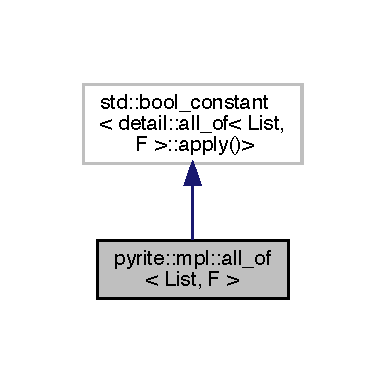
\includegraphics[width=185pt]{da/de9/structpyrite_1_1mpl_1_1all__of__inherit__graph}
\end{center}
\end{figure}


Collaboration diagram for pyrite\+:\+:mpl\+:\+:all\+\_\+of$<$ List, F $>$\+:
\nopagebreak
\begin{figure}[H]
\begin{center}
\leavevmode
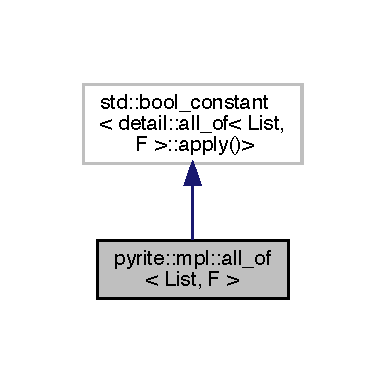
\includegraphics[width=185pt]{d7/d84/structpyrite_1_1mpl_1_1all__of__coll__graph}
\end{center}
\end{figure}


The documentation for this struct was generated from the following file\+:\begin{DoxyCompactItemize}
\item 
/\+Users/masato.\+tanaka/\+Development/cpp/pyrite/pyrite/mpl/type\+\_\+list/\mbox{\hyperlink{all__of_8hpp}{all\+\_\+of.\+hpp}}\end{DoxyCompactItemize}

\hypertarget{classpyrite_1_1math_1_1angle}{}\section{pyrite\+:\+:math\+:\+:angle$<$ T $>$ Class Template Reference}
\label{classpyrite_1_1math_1_1angle}\index{pyrite\+::math\+::angle$<$ T $>$@{pyrite\+::math\+::angle$<$ T $>$}}
\subsection*{Public Types}
\begin{DoxyCompactItemize}
\item 
\mbox{\Hypertarget{classpyrite_1_1math_1_1angle_addf4eff8f082fbbbd99babed3e19271f}\label{classpyrite_1_1math_1_1angle_addf4eff8f082fbbbd99babed3e19271f}} 
using \mbox{\hyperlink{classpyrite_1_1math_1_1angle_addf4eff8f082fbbbd99babed3e19271f}{value\+\_\+type}} = T
\begin{DoxyCompactList}\small\item\em value type (T) \end{DoxyCompactList}\end{DoxyCompactItemize}
\subsection*{Public Member Functions}
\begin{DoxyCompactItemize}
\item 
constexpr \mbox{\hyperlink{classpyrite_1_1math_1_1angle_a391868de4c78d823cf4a55373e28b90c}{angle}} () noexcept=default
\item 
constexpr \mbox{\hyperlink{classpyrite_1_1math_1_1angle_a2c9aeede6bd0edf739a440515ea20f0c}{angle}} (T const \&rad, \mbox{\hyperlink{structpyrite_1_1math_1_1radian__angle__tag__t}{radian\+\_\+angle\+\_\+tag\+\_\+t}})
\item 
constexpr \mbox{\hyperlink{classpyrite_1_1math_1_1angle_ab983c2beb0c1c127844dd437ffb5a6d6}{angle}} (T const \&deg, \mbox{\hyperlink{structpyrite_1_1math_1_1degree__angle__tag__t}{degree\+\_\+angle\+\_\+tag\+\_\+t}})
\item 
constexpr \mbox{\hyperlink{classpyrite_1_1math_1_1angle_a82354ef1bc05d04bc73c3959f30147c6}{angle}} (\mbox{\hyperlink{classpyrite_1_1math_1_1angle}{angle}} const \&other)
\item 
constexpr \mbox{\hyperlink{classpyrite_1_1math_1_1angle_a7aeda1e3d5aa652daf62bc0aeff89245}{angle}} (\mbox{\hyperlink{classpyrite_1_1math_1_1angle}{angle}} \&\&other)=default
\item 
\mbox{\hyperlink{classpyrite_1_1math_1_1angle_a53b066dbf9792cf5483ab6665a0f31da}{$\sim$angle}} ()=default
\item 
constexpr \mbox{\hyperlink{classpyrite_1_1math_1_1angle}{angle}} \& \mbox{\hyperlink{classpyrite_1_1math_1_1angle_a3beefc40aadf5528ee5fd76823d98420}{rotate}} (\mbox{\hyperlink{classpyrite_1_1math_1_1angle}{angle}} const \&other)
\item 
constexpr \mbox{\hyperlink{classpyrite_1_1math_1_1angle}{angle}} \& \mbox{\hyperlink{classpyrite_1_1math_1_1angle_a2fab8f4261d509f5272e9f9ebec19028}{radian}} (T const \&rad)
\item 
constexpr \mbox{\hyperlink{classpyrite_1_1math_1_1angle}{angle}} \& \mbox{\hyperlink{classpyrite_1_1math_1_1angle_a7e27daa8c8cb81986a146495664dfaba}{degree}} (T const \&deg)
\item 
constexpr T \mbox{\hyperlink{classpyrite_1_1math_1_1angle_a01c42dc88f49b1b945e187aa2c5f190a}{radian}} () const noexcept
\item 
constexpr T \mbox{\hyperlink{classpyrite_1_1math_1_1angle_a52d68b9f0b2bedfed7fa09782dba0e82}{degree}} () const noexcept
\item 
constexpr T \mbox{\hyperlink{classpyrite_1_1math_1_1angle_a52b2bed9f8df78271f96ee0c79f8c8a8}{sin}} () const
\item 
constexpr T \mbox{\hyperlink{classpyrite_1_1math_1_1angle_a5126aac02ec54f94df6aecac8e9d9e9a}{cos}} () const
\item 
constexpr T \mbox{\hyperlink{classpyrite_1_1math_1_1angle_a1d63fa42bc9004aa686fe2992f235ebb}{tan}} () const
\item 
constexpr \mbox{\hyperlink{classpyrite_1_1math_1_1angle}{angle}} \& \mbox{\hyperlink{classpyrite_1_1math_1_1angle_aaa7837421f293c5d2938442efcd6cc02}{operator=}} (\mbox{\hyperlink{classpyrite_1_1math_1_1angle}{angle}} const \&other) noexcept
\item 
constexpr \mbox{\hyperlink{classpyrite_1_1math_1_1angle}{angle}} \& \mbox{\hyperlink{classpyrite_1_1math_1_1angle_acf9aa48fe206f5bdc202479bb9f0354a}{operator=}} (\mbox{\hyperlink{classpyrite_1_1math_1_1angle}{angle}} \&\&other) noexcept
\end{DoxyCompactItemize}
\subsection*{Friends}
\begin{DoxyCompactItemize}
\item 
\mbox{\Hypertarget{classpyrite_1_1math_1_1angle_aace8cc4c31692174ca8d9644007743e8}\label{classpyrite_1_1math_1_1angle_aace8cc4c31692174ca8d9644007743e8}} 
constexpr \mbox{\hyperlink{classpyrite_1_1math_1_1angle}{angle}} {\bfseries operator+} (\mbox{\hyperlink{classpyrite_1_1math_1_1angle}{angle}} const \&a)
\item 
\mbox{\Hypertarget{classpyrite_1_1math_1_1angle_af42bd0fef2d808bddfc3d271f53f8838}\label{classpyrite_1_1math_1_1angle_af42bd0fef2d808bddfc3d271f53f8838}} 
constexpr \mbox{\hyperlink{classpyrite_1_1math_1_1angle}{angle}} {\bfseries operator-\/} (\mbox{\hyperlink{classpyrite_1_1math_1_1angle}{angle}} const \&a)
\item 
\mbox{\Hypertarget{classpyrite_1_1math_1_1angle_a45f3de0aaf46d319c018f0b5e52c9cc8}\label{classpyrite_1_1math_1_1angle_a45f3de0aaf46d319c018f0b5e52c9cc8}} 
constexpr \mbox{\hyperlink{classpyrite_1_1math_1_1angle}{angle}} \& {\bfseries operator+=} (\mbox{\hyperlink{classpyrite_1_1math_1_1angle}{angle}} \&lhs, \mbox{\hyperlink{classpyrite_1_1math_1_1angle}{angle}} const \&rhs)
\item 
\mbox{\Hypertarget{classpyrite_1_1math_1_1angle_ad088ca5eac35b4e997dd84f90002801e}\label{classpyrite_1_1math_1_1angle_ad088ca5eac35b4e997dd84f90002801e}} 
constexpr \mbox{\hyperlink{classpyrite_1_1math_1_1angle}{angle}} \& {\bfseries operator-\/=} (\mbox{\hyperlink{classpyrite_1_1math_1_1angle}{angle}} \&lhs, \mbox{\hyperlink{classpyrite_1_1math_1_1angle}{angle}} const \&rhs)
\item 
\mbox{\Hypertarget{classpyrite_1_1math_1_1angle_a2d582706b0ff59dc60fbc2a426f9994e}\label{classpyrite_1_1math_1_1angle_a2d582706b0ff59dc60fbc2a426f9994e}} 
constexpr \mbox{\hyperlink{classpyrite_1_1math_1_1angle}{angle}} \& {\bfseries operator$\ast$=} (\mbox{\hyperlink{classpyrite_1_1math_1_1angle}{angle}} \&a, T const \&value)
\item 
\mbox{\Hypertarget{classpyrite_1_1math_1_1angle_a1354205c05bea757c2ac060a0e6c043b}\label{classpyrite_1_1math_1_1angle_a1354205c05bea757c2ac060a0e6c043b}} 
constexpr \mbox{\hyperlink{classpyrite_1_1math_1_1angle}{angle}} \& {\bfseries operator/=} (\mbox{\hyperlink{classpyrite_1_1math_1_1angle}{angle}} \&a, T const \&value)
\item 
\mbox{\Hypertarget{classpyrite_1_1math_1_1angle_ad7e212aae809d81ca45e388d6bb03b8b}\label{classpyrite_1_1math_1_1angle_ad7e212aae809d81ca45e388d6bb03b8b}} 
constexpr \mbox{\hyperlink{classpyrite_1_1math_1_1angle}{angle}} {\bfseries operator+} (\mbox{\hyperlink{classpyrite_1_1math_1_1angle}{angle}} const \&lhs, \mbox{\hyperlink{classpyrite_1_1math_1_1angle}{angle}} const \&rhs)
\item 
\mbox{\Hypertarget{classpyrite_1_1math_1_1angle_a65bde81f1eb8cc2c555ff0e9a2d8905b}\label{classpyrite_1_1math_1_1angle_a65bde81f1eb8cc2c555ff0e9a2d8905b}} 
constexpr \mbox{\hyperlink{classpyrite_1_1math_1_1angle}{angle}} {\bfseries operator-\/} (\mbox{\hyperlink{classpyrite_1_1math_1_1angle}{angle}} const \&lhs, \mbox{\hyperlink{classpyrite_1_1math_1_1angle}{angle}} const \&rhs)
\item 
\mbox{\Hypertarget{classpyrite_1_1math_1_1angle_a3708ed238352b0c5f5e2ba5ccc7023af}\label{classpyrite_1_1math_1_1angle_a3708ed238352b0c5f5e2ba5ccc7023af}} 
constexpr \mbox{\hyperlink{classpyrite_1_1math_1_1angle}{angle}} {\bfseries operator$\ast$} (\mbox{\hyperlink{classpyrite_1_1math_1_1angle}{angle}} const \&a, T const \&value)
\item 
\mbox{\Hypertarget{classpyrite_1_1math_1_1angle_ab682a83b8b349e46e201fa91d2952058}\label{classpyrite_1_1math_1_1angle_ab682a83b8b349e46e201fa91d2952058}} 
constexpr \mbox{\hyperlink{classpyrite_1_1math_1_1angle}{angle}} {\bfseries operator/} (\mbox{\hyperlink{classpyrite_1_1math_1_1angle}{angle}} const \&a, T const \&value)
\item 
\mbox{\Hypertarget{classpyrite_1_1math_1_1angle_a064c0db187ddd7b8f2176d795cd2ba4d}\label{classpyrite_1_1math_1_1angle_a064c0db187ddd7b8f2176d795cd2ba4d}} 
constexpr \mbox{\hyperlink{classpyrite_1_1math_1_1angle}{angle}} {\bfseries operator$\ast$} (T const \&value, \mbox{\hyperlink{classpyrite_1_1math_1_1angle}{angle}} const \&a)
\item 
\mbox{\Hypertarget{classpyrite_1_1math_1_1angle_adb210ba2c06aaeb7ffaacee6324e1b3b}\label{classpyrite_1_1math_1_1angle_adb210ba2c06aaeb7ffaacee6324e1b3b}} 
constexpr bool {\bfseries operator==} (\mbox{\hyperlink{classpyrite_1_1math_1_1angle}{angle}} const \&lhs, \mbox{\hyperlink{classpyrite_1_1math_1_1angle}{angle}} const \&rhs) noexcept
\item 
\mbox{\Hypertarget{classpyrite_1_1math_1_1angle_a6d08791f36b9be1cb0a5b06ec4be223f}\label{classpyrite_1_1math_1_1angle_a6d08791f36b9be1cb0a5b06ec4be223f}} 
constexpr bool {\bfseries operator!=} (\mbox{\hyperlink{classpyrite_1_1math_1_1angle}{angle}} const \&lhs, \mbox{\hyperlink{classpyrite_1_1math_1_1angle}{angle}} const \&rhs) noexcept
\item 
\mbox{\Hypertarget{classpyrite_1_1math_1_1angle_ad7c85186c2bebde44aacc2a5df292a9d}\label{classpyrite_1_1math_1_1angle_ad7c85186c2bebde44aacc2a5df292a9d}} 
constexpr bool {\bfseries operator$<$} (\mbox{\hyperlink{classpyrite_1_1math_1_1angle}{angle}} const \&lhs, \mbox{\hyperlink{classpyrite_1_1math_1_1angle}{angle}} const \&rhs) noexcept
\item 
\mbox{\Hypertarget{classpyrite_1_1math_1_1angle_a50372b5d3853f13f11293ca14721cc84}\label{classpyrite_1_1math_1_1angle_a50372b5d3853f13f11293ca14721cc84}} 
constexpr bool {\bfseries operator$<$=} (\mbox{\hyperlink{classpyrite_1_1math_1_1angle}{angle}} const \&lhs, \mbox{\hyperlink{classpyrite_1_1math_1_1angle}{angle}} const \&rhs) noexcept
\item 
\mbox{\Hypertarget{classpyrite_1_1math_1_1angle_a30ca63b1b25a49492042530ee60ed4ef}\label{classpyrite_1_1math_1_1angle_a30ca63b1b25a49492042530ee60ed4ef}} 
constexpr bool {\bfseries operator$>$} (\mbox{\hyperlink{classpyrite_1_1math_1_1angle}{angle}} const \&lhs, \mbox{\hyperlink{classpyrite_1_1math_1_1angle}{angle}} const \&rhs) noexcept
\item 
\mbox{\Hypertarget{classpyrite_1_1math_1_1angle_ac7bef78cbae62dbe5b8a16e61a3101de}\label{classpyrite_1_1math_1_1angle_ac7bef78cbae62dbe5b8a16e61a3101de}} 
constexpr bool {\bfseries operator$>$=} (\mbox{\hyperlink{classpyrite_1_1math_1_1angle}{angle}} const \&lhs, \mbox{\hyperlink{classpyrite_1_1math_1_1angle}{angle}} const \&rhs) noexcept
\end{DoxyCompactItemize}


\subsection{Constructor \& Destructor Documentation}
\mbox{\Hypertarget{classpyrite_1_1math_1_1angle_a391868de4c78d823cf4a55373e28b90c}\label{classpyrite_1_1math_1_1angle_a391868de4c78d823cf4a55373e28b90c}} 
\index{pyrite\+::math\+::angle@{pyrite\+::math\+::angle}!angle@{angle}}
\index{angle@{angle}!pyrite\+::math\+::angle@{pyrite\+::math\+::angle}}
\subsubsection{\texorpdfstring{angle()}{angle()}\hspace{0.1cm}{\footnotesize\ttfamily [1/5]}}
{\footnotesize\ttfamily template$<$typename T $>$ \\
constexpr \mbox{\hyperlink{classpyrite_1_1math_1_1angle}{pyrite\+::math\+::angle}}$<$ T $>$\+::\mbox{\hyperlink{classpyrite_1_1math_1_1angle}{angle}} (\begin{DoxyParamCaption}{ }\end{DoxyParamCaption})\hspace{0.3cm}{\ttfamily [default]}, {\ttfamily [noexcept]}}

default constructor. \mbox{\Hypertarget{classpyrite_1_1math_1_1angle_a2c9aeede6bd0edf739a440515ea20f0c}\label{classpyrite_1_1math_1_1angle_a2c9aeede6bd0edf739a440515ea20f0c}} 
\index{pyrite\+::math\+::angle@{pyrite\+::math\+::angle}!angle@{angle}}
\index{angle@{angle}!pyrite\+::math\+::angle@{pyrite\+::math\+::angle}}
\subsubsection{\texorpdfstring{angle()}{angle()}\hspace{0.1cm}{\footnotesize\ttfamily [2/5]}}
{\footnotesize\ttfamily template$<$typename T $>$ \\
constexpr \mbox{\hyperlink{classpyrite_1_1math_1_1angle}{pyrite\+::math\+::angle}}$<$ T $>$\+::\mbox{\hyperlink{classpyrite_1_1math_1_1angle}{angle}} (\begin{DoxyParamCaption}\item[{T const \&}]{rad,  }\item[{\mbox{\hyperlink{structpyrite_1_1math_1_1radian__angle__tag__t}{radian\+\_\+angle\+\_\+tag\+\_\+t}}}]{ }\end{DoxyParamCaption})\hspace{0.3cm}{\ttfamily [inline]}}

constructs the angle from radian.


\begin{DoxyParams}[1]{Parameters}
\mbox{\tt in}  & {\em rad} & radian. \\
\hline
\end{DoxyParams}
\mbox{\Hypertarget{classpyrite_1_1math_1_1angle_ab983c2beb0c1c127844dd437ffb5a6d6}\label{classpyrite_1_1math_1_1angle_ab983c2beb0c1c127844dd437ffb5a6d6}} 
\index{pyrite\+::math\+::angle@{pyrite\+::math\+::angle}!angle@{angle}}
\index{angle@{angle}!pyrite\+::math\+::angle@{pyrite\+::math\+::angle}}
\subsubsection{\texorpdfstring{angle()}{angle()}\hspace{0.1cm}{\footnotesize\ttfamily [3/5]}}
{\footnotesize\ttfamily template$<$typename T $>$ \\
constexpr \mbox{\hyperlink{classpyrite_1_1math_1_1angle}{pyrite\+::math\+::angle}}$<$ T $>$\+::\mbox{\hyperlink{classpyrite_1_1math_1_1angle}{angle}} (\begin{DoxyParamCaption}\item[{T const \&}]{deg,  }\item[{\mbox{\hyperlink{structpyrite_1_1math_1_1degree__angle__tag__t}{degree\+\_\+angle\+\_\+tag\+\_\+t}}}]{ }\end{DoxyParamCaption})\hspace{0.3cm}{\ttfamily [inline]}}

constructs the angle from degree.


\begin{DoxyParams}[1]{Parameters}
\mbox{\tt in}  & {\em deg} & degree. \\
\hline
\end{DoxyParams}
Here is the call graph for this function\+:
\nopagebreak
\begin{figure}[H]
\begin{center}
\leavevmode
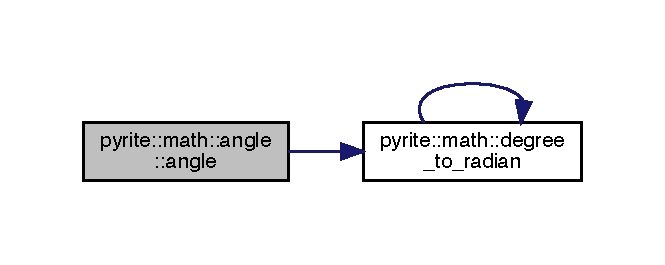
\includegraphics[width=319pt]{d0/df1/classpyrite_1_1math_1_1angle_ab983c2beb0c1c127844dd437ffb5a6d6_cgraph}
\end{center}
\end{figure}
\mbox{\Hypertarget{classpyrite_1_1math_1_1angle_a82354ef1bc05d04bc73c3959f30147c6}\label{classpyrite_1_1math_1_1angle_a82354ef1bc05d04bc73c3959f30147c6}} 
\index{pyrite\+::math\+::angle@{pyrite\+::math\+::angle}!angle@{angle}}
\index{angle@{angle}!pyrite\+::math\+::angle@{pyrite\+::math\+::angle}}
\subsubsection{\texorpdfstring{angle()}{angle()}\hspace{0.1cm}{\footnotesize\ttfamily [4/5]}}
{\footnotesize\ttfamily template$<$typename T $>$ \\
constexpr \mbox{\hyperlink{classpyrite_1_1math_1_1angle}{pyrite\+::math\+::angle}}$<$ T $>$\+::\mbox{\hyperlink{classpyrite_1_1math_1_1angle}{angle}} (\begin{DoxyParamCaption}\item[{\mbox{\hyperlink{classpyrite_1_1math_1_1angle}{angle}}$<$ T $>$ const \&}]{other }\end{DoxyParamCaption})\hspace{0.3cm}{\ttfamily [inline]}}

copy constrcutor.


\begin{DoxyParams}[1]{Parameters}
\mbox{\tt in}  & {\em other} & source. \\
\hline
\end{DoxyParams}
\mbox{\Hypertarget{classpyrite_1_1math_1_1angle_a7aeda1e3d5aa652daf62bc0aeff89245}\label{classpyrite_1_1math_1_1angle_a7aeda1e3d5aa652daf62bc0aeff89245}} 
\index{pyrite\+::math\+::angle@{pyrite\+::math\+::angle}!angle@{angle}}
\index{angle@{angle}!pyrite\+::math\+::angle@{pyrite\+::math\+::angle}}
\subsubsection{\texorpdfstring{angle()}{angle()}\hspace{0.1cm}{\footnotesize\ttfamily [5/5]}}
{\footnotesize\ttfamily template$<$typename T $>$ \\
constexpr \mbox{\hyperlink{classpyrite_1_1math_1_1angle}{pyrite\+::math\+::angle}}$<$ T $>$\+::\mbox{\hyperlink{classpyrite_1_1math_1_1angle}{angle}} (\begin{DoxyParamCaption}\item[{\mbox{\hyperlink{classpyrite_1_1math_1_1angle}{angle}}$<$ T $>$ \&\&}]{other }\end{DoxyParamCaption})\hspace{0.3cm}{\ttfamily [default]}}

move constrcutor.


\begin{DoxyParams}[1]{Parameters}
\mbox{\tt in}  & {\em other} & source. \\
\hline
\end{DoxyParams}
\mbox{\Hypertarget{classpyrite_1_1math_1_1angle_a53b066dbf9792cf5483ab6665a0f31da}\label{classpyrite_1_1math_1_1angle_a53b066dbf9792cf5483ab6665a0f31da}} 
\index{pyrite\+::math\+::angle@{pyrite\+::math\+::angle}!````~angle@{$\sim$angle}}
\index{````~angle@{$\sim$angle}!pyrite\+::math\+::angle@{pyrite\+::math\+::angle}}
\subsubsection{\texorpdfstring{$\sim$angle()}{~angle()}}
{\footnotesize\ttfamily template$<$typename T $>$ \\
\mbox{\hyperlink{classpyrite_1_1math_1_1angle}{pyrite\+::math\+::angle}}$<$ T $>$\+::$\sim$\mbox{\hyperlink{classpyrite_1_1math_1_1angle}{angle}} (\begin{DoxyParamCaption}{ }\end{DoxyParamCaption})\hspace{0.3cm}{\ttfamily [default]}}

destructor. generated form compiler.


\begin{DoxyParams}[1]{Parameters}
\mbox{\tt in}  & {\em other} & source. \\
\hline
\end{DoxyParams}


\subsection{Member Function Documentation}
\mbox{\Hypertarget{classpyrite_1_1math_1_1angle_a5126aac02ec54f94df6aecac8e9d9e9a}\label{classpyrite_1_1math_1_1angle_a5126aac02ec54f94df6aecac8e9d9e9a}} 
\index{pyrite\+::math\+::angle@{pyrite\+::math\+::angle}!cos@{cos}}
\index{cos@{cos}!pyrite\+::math\+::angle@{pyrite\+::math\+::angle}}
\subsubsection{\texorpdfstring{cos()}{cos()}}
{\footnotesize\ttfamily template$<$typename T $>$ \\
constexpr T \mbox{\hyperlink{classpyrite_1_1math_1_1angle}{pyrite\+::math\+::angle}}$<$ T $>$\+::cos (\begin{DoxyParamCaption}{ }\end{DoxyParamCaption}) const\hspace{0.3cm}{\ttfamily [inline]}}

get cos(radian()). \begin{DoxyReturn}{Returns}
cos(radian()). 
\end{DoxyReturn}
\mbox{\Hypertarget{classpyrite_1_1math_1_1angle_a7e27daa8c8cb81986a146495664dfaba}\label{classpyrite_1_1math_1_1angle_a7e27daa8c8cb81986a146495664dfaba}} 
\index{pyrite\+::math\+::angle@{pyrite\+::math\+::angle}!degree@{degree}}
\index{degree@{degree}!pyrite\+::math\+::angle@{pyrite\+::math\+::angle}}
\subsubsection{\texorpdfstring{degree()}{degree()}\hspace{0.1cm}{\footnotesize\ttfamily [1/2]}}
{\footnotesize\ttfamily template$<$typename T $>$ \\
constexpr \mbox{\hyperlink{classpyrite_1_1math_1_1angle}{angle}}\& \mbox{\hyperlink{classpyrite_1_1math_1_1angle}{pyrite\+::math\+::angle}}$<$ T $>$\+::degree (\begin{DoxyParamCaption}\item[{T const \&}]{deg }\end{DoxyParamCaption})\hspace{0.3cm}{\ttfamily [inline]}}

set value from degree.


\begin{DoxyParams}[1]{Parameters}
\mbox{\tt in}  & {\em deg} & degree. \\
\hline
\end{DoxyParams}
\begin{DoxyReturn}{Returns}
return the result by reference. 
\end{DoxyReturn}
Here is the call graph for this function\+:
\nopagebreak
\begin{figure}[H]
\begin{center}
\leavevmode
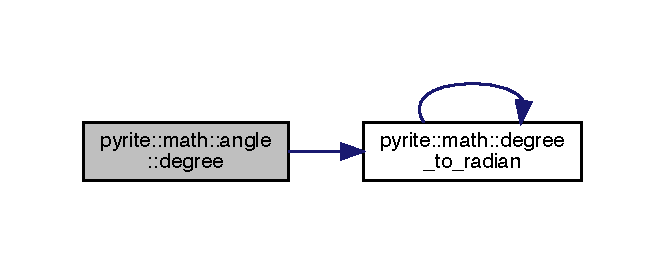
\includegraphics[width=319pt]{d0/df1/classpyrite_1_1math_1_1angle_a7e27daa8c8cb81986a146495664dfaba_cgraph}
\end{center}
\end{figure}
\mbox{\Hypertarget{classpyrite_1_1math_1_1angle_a52d68b9f0b2bedfed7fa09782dba0e82}\label{classpyrite_1_1math_1_1angle_a52d68b9f0b2bedfed7fa09782dba0e82}} 
\index{pyrite\+::math\+::angle@{pyrite\+::math\+::angle}!degree@{degree}}
\index{degree@{degree}!pyrite\+::math\+::angle@{pyrite\+::math\+::angle}}
\subsubsection{\texorpdfstring{degree()}{degree()}\hspace{0.1cm}{\footnotesize\ttfamily [2/2]}}
{\footnotesize\ttfamily template$<$typename T $>$ \\
constexpr T \mbox{\hyperlink{classpyrite_1_1math_1_1angle}{pyrite\+::math\+::angle}}$<$ T $>$\+::degree (\begin{DoxyParamCaption}{ }\end{DoxyParamCaption}) const\hspace{0.3cm}{\ttfamily [inline]}, {\ttfamily [noexcept]}}

get value of degree. \begin{DoxyReturn}{Returns}
degree. 
\end{DoxyReturn}
Here is the call graph for this function\+:
\nopagebreak
\begin{figure}[H]
\begin{center}
\leavevmode
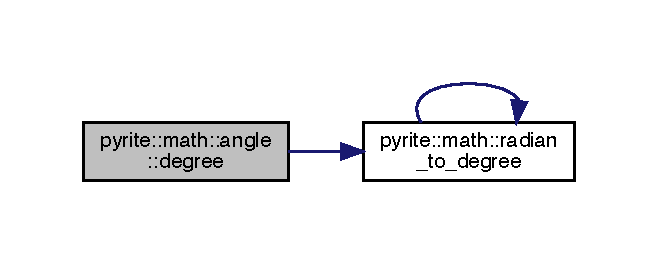
\includegraphics[width=316pt]{d0/df1/classpyrite_1_1math_1_1angle_a52d68b9f0b2bedfed7fa09782dba0e82_cgraph}
\end{center}
\end{figure}
\mbox{\Hypertarget{classpyrite_1_1math_1_1angle_aaa7837421f293c5d2938442efcd6cc02}\label{classpyrite_1_1math_1_1angle_aaa7837421f293c5d2938442efcd6cc02}} 
\index{pyrite\+::math\+::angle@{pyrite\+::math\+::angle}!operator=@{operator=}}
\index{operator=@{operator=}!pyrite\+::math\+::angle@{pyrite\+::math\+::angle}}
\subsubsection{\texorpdfstring{operator=()}{operator=()}\hspace{0.1cm}{\footnotesize\ttfamily [1/2]}}
{\footnotesize\ttfamily template$<$typename T $>$ \\
constexpr \mbox{\hyperlink{classpyrite_1_1math_1_1angle}{angle}}\& \mbox{\hyperlink{classpyrite_1_1math_1_1angle}{pyrite\+::math\+::angle}}$<$ T $>$\+::operator= (\begin{DoxyParamCaption}\item[{\mbox{\hyperlink{classpyrite_1_1math_1_1angle}{angle}}$<$ T $>$ const \&}]{other }\end{DoxyParamCaption})\hspace{0.3cm}{\ttfamily [inline]}, {\ttfamily [noexcept]}}

copy assignment operator.


\begin{DoxyParams}{Parameters}
{\em other} & source. \\
\hline
\end{DoxyParams}
\begin{DoxyReturn}{Returns}
return the result by reference. 
\end{DoxyReturn}
\mbox{\Hypertarget{classpyrite_1_1math_1_1angle_acf9aa48fe206f5bdc202479bb9f0354a}\label{classpyrite_1_1math_1_1angle_acf9aa48fe206f5bdc202479bb9f0354a}} 
\index{pyrite\+::math\+::angle@{pyrite\+::math\+::angle}!operator=@{operator=}}
\index{operator=@{operator=}!pyrite\+::math\+::angle@{pyrite\+::math\+::angle}}
\subsubsection{\texorpdfstring{operator=()}{operator=()}\hspace{0.1cm}{\footnotesize\ttfamily [2/2]}}
{\footnotesize\ttfamily template$<$typename T $>$ \\
constexpr \mbox{\hyperlink{classpyrite_1_1math_1_1angle}{angle}}\& \mbox{\hyperlink{classpyrite_1_1math_1_1angle}{pyrite\+::math\+::angle}}$<$ T $>$\+::operator= (\begin{DoxyParamCaption}\item[{\mbox{\hyperlink{classpyrite_1_1math_1_1angle}{angle}}$<$ T $>$ \&\&}]{other }\end{DoxyParamCaption})\hspace{0.3cm}{\ttfamily [inline]}, {\ttfamily [noexcept]}}

move assignment operator.


\begin{DoxyParams}{Parameters}
{\em other} & source. \\
\hline
\end{DoxyParams}
\begin{DoxyReturn}{Returns}
return the result by reference. 
\end{DoxyReturn}
\mbox{\Hypertarget{classpyrite_1_1math_1_1angle_a2fab8f4261d509f5272e9f9ebec19028}\label{classpyrite_1_1math_1_1angle_a2fab8f4261d509f5272e9f9ebec19028}} 
\index{pyrite\+::math\+::angle@{pyrite\+::math\+::angle}!radian@{radian}}
\index{radian@{radian}!pyrite\+::math\+::angle@{pyrite\+::math\+::angle}}
\subsubsection{\texorpdfstring{radian()}{radian()}\hspace{0.1cm}{\footnotesize\ttfamily [1/2]}}
{\footnotesize\ttfamily template$<$typename T $>$ \\
constexpr \mbox{\hyperlink{classpyrite_1_1math_1_1angle}{angle}}\& \mbox{\hyperlink{classpyrite_1_1math_1_1angle}{pyrite\+::math\+::angle}}$<$ T $>$\+::radian (\begin{DoxyParamCaption}\item[{T const \&}]{rad }\end{DoxyParamCaption})\hspace{0.3cm}{\ttfamily [inline]}}

set value form radian.


\begin{DoxyParams}[1]{Parameters}
\mbox{\tt in}  & {\em rad} & radian. \\
\hline
\end{DoxyParams}
\begin{DoxyReturn}{Returns}
return the result by reference. 
\end{DoxyReturn}
\mbox{\Hypertarget{classpyrite_1_1math_1_1angle_a01c42dc88f49b1b945e187aa2c5f190a}\label{classpyrite_1_1math_1_1angle_a01c42dc88f49b1b945e187aa2c5f190a}} 
\index{pyrite\+::math\+::angle@{pyrite\+::math\+::angle}!radian@{radian}}
\index{radian@{radian}!pyrite\+::math\+::angle@{pyrite\+::math\+::angle}}
\subsubsection{\texorpdfstring{radian()}{radian()}\hspace{0.1cm}{\footnotesize\ttfamily [2/2]}}
{\footnotesize\ttfamily template$<$typename T $>$ \\
constexpr T \mbox{\hyperlink{classpyrite_1_1math_1_1angle}{pyrite\+::math\+::angle}}$<$ T $>$\+::radian (\begin{DoxyParamCaption}{ }\end{DoxyParamCaption}) const\hspace{0.3cm}{\ttfamily [inline]}, {\ttfamily [noexcept]}}

get value of radian. \begin{DoxyReturn}{Returns}
radian. 
\end{DoxyReturn}
\mbox{\Hypertarget{classpyrite_1_1math_1_1angle_a3beefc40aadf5528ee5fd76823d98420}\label{classpyrite_1_1math_1_1angle_a3beefc40aadf5528ee5fd76823d98420}} 
\index{pyrite\+::math\+::angle@{pyrite\+::math\+::angle}!rotate@{rotate}}
\index{rotate@{rotate}!pyrite\+::math\+::angle@{pyrite\+::math\+::angle}}
\subsubsection{\texorpdfstring{rotate()}{rotate()}}
{\footnotesize\ttfamily template$<$typename T $>$ \\
constexpr \mbox{\hyperlink{classpyrite_1_1math_1_1angle}{angle}}\& \mbox{\hyperlink{classpyrite_1_1math_1_1angle}{pyrite\+::math\+::angle}}$<$ T $>$\+::rotate (\begin{DoxyParamCaption}\item[{\mbox{\hyperlink{classpyrite_1_1math_1_1angle}{angle}}$<$ T $>$ const \&}]{other }\end{DoxyParamCaption})\hspace{0.3cm}{\ttfamily [inline]}}

rotate angle object


\begin{DoxyParams}[1]{Parameters}
\mbox{\tt in}  & {\em other} & add angle. \\
\hline
\end{DoxyParams}
\begin{DoxyReturn}{Returns}
reference 
\end{DoxyReturn}
\mbox{\Hypertarget{classpyrite_1_1math_1_1angle_a52b2bed9f8df78271f96ee0c79f8c8a8}\label{classpyrite_1_1math_1_1angle_a52b2bed9f8df78271f96ee0c79f8c8a8}} 
\index{pyrite\+::math\+::angle@{pyrite\+::math\+::angle}!sin@{sin}}
\index{sin@{sin}!pyrite\+::math\+::angle@{pyrite\+::math\+::angle}}
\subsubsection{\texorpdfstring{sin()}{sin()}}
{\footnotesize\ttfamily template$<$typename T $>$ \\
constexpr T \mbox{\hyperlink{classpyrite_1_1math_1_1angle}{pyrite\+::math\+::angle}}$<$ T $>$\+::sin (\begin{DoxyParamCaption}{ }\end{DoxyParamCaption}) const\hspace{0.3cm}{\ttfamily [inline]}}

get sin(radian()). \begin{DoxyReturn}{Returns}
sin(radian()). 
\end{DoxyReturn}
\mbox{\Hypertarget{classpyrite_1_1math_1_1angle_a1d63fa42bc9004aa686fe2992f235ebb}\label{classpyrite_1_1math_1_1angle_a1d63fa42bc9004aa686fe2992f235ebb}} 
\index{pyrite\+::math\+::angle@{pyrite\+::math\+::angle}!tan@{tan}}
\index{tan@{tan}!pyrite\+::math\+::angle@{pyrite\+::math\+::angle}}
\subsubsection{\texorpdfstring{tan()}{tan()}}
{\footnotesize\ttfamily template$<$typename T $>$ \\
constexpr T \mbox{\hyperlink{classpyrite_1_1math_1_1angle}{pyrite\+::math\+::angle}}$<$ T $>$\+::tan (\begin{DoxyParamCaption}{ }\end{DoxyParamCaption}) const\hspace{0.3cm}{\ttfamily [inline]}}

get tan(radian()). \begin{DoxyReturn}{Returns}
tan(radian()). 
\end{DoxyReturn}


The documentation for this class was generated from the following file\+:\begin{DoxyCompactItemize}
\item 
/\+Users/masato.\+tanaka/\+Development/cpp/pyrite/pyrite/math/\mbox{\hyperlink{angle_8hpp}{angle.\+hpp}}\end{DoxyCompactItemize}

\hypertarget{structpyrite_1_1mpl_1_1any__of}{}\section{pyrite\+:\+:mpl\+:\+:any\+\_\+of$<$ List, F $>$ Struct Template Reference}
\label{structpyrite_1_1mpl_1_1any__of}\index{pyrite\+::mpl\+::any\+\_\+of$<$ List, F $>$@{pyrite\+::mpl\+::any\+\_\+of$<$ List, F $>$}}


Inheritance diagram for pyrite\+:\+:mpl\+:\+:any\+\_\+of$<$ List, F $>$\+:
\nopagebreak
\begin{figure}[H]
\begin{center}
\leavevmode
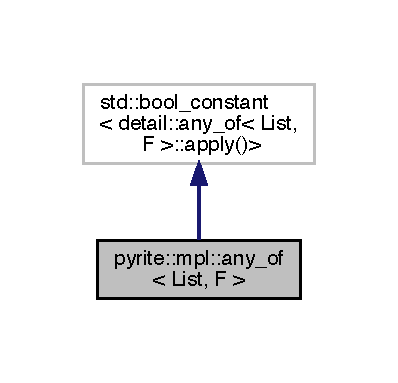
\includegraphics[width=191pt]{d4/df2/structpyrite_1_1mpl_1_1any__of__inherit__graph}
\end{center}
\end{figure}


Collaboration diagram for pyrite\+:\+:mpl\+:\+:any\+\_\+of$<$ List, F $>$\+:
\nopagebreak
\begin{figure}[H]
\begin{center}
\leavevmode
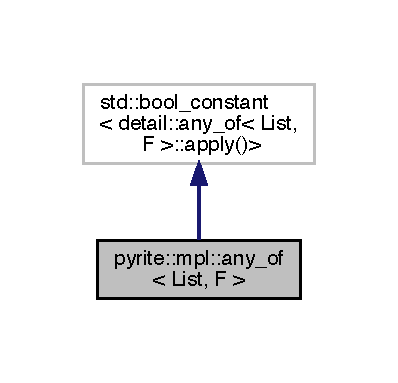
\includegraphics[width=191pt]{d8/d6d/structpyrite_1_1mpl_1_1any__of__coll__graph}
\end{center}
\end{figure}


The documentation for this struct was generated from the following file\+:\begin{DoxyCompactItemize}
\item 
/\+Users/masato.\+tanaka/\+Development/cpp/pyrite/pyrite/mpl/type\+\_\+list/\mbox{\hyperlink{any__of_8hpp}{any\+\_\+of.\+hpp}}\end{DoxyCompactItemize}

\hypertarget{structpyrite_1_1mpl_1_1at}{}\section{pyrite\+:\+:mpl\+:\+:at$<$ List, Index $>$ Struct Template Reference}
\label{structpyrite_1_1mpl_1_1at}\index{pyrite\+::mpl\+::at$<$ List, Index $>$@{pyrite\+::mpl\+::at$<$ List, Index $>$}}
\subsection*{Public Types}
\begin{DoxyCompactItemize}
\item 
\mbox{\Hypertarget{structpyrite_1_1mpl_1_1at_a8bba5ea8c51859e7ba730264c20d7603}\label{structpyrite_1_1mpl_1_1at_a8bba5ea8c51859e7ba730264c20d7603}} 
using {\bfseries type} = typename founded\+\_\+pair\+\_\+optional\+::type\+::first
\end{DoxyCompactItemize}


The documentation for this struct was generated from the following file\+:\begin{DoxyCompactItemize}
\item 
/\+Users/masato.\+tanaka/\+Development/cpp/pyrite/pyrite/mpl/type\+\_\+list/\mbox{\hyperlink{at_8hpp}{at.\+hpp}}\end{DoxyCompactItemize}

\hypertarget{classpyrite_1_1core_1_1checked__array__deleter}{}\section{pyrite\+:\+:core\+:\+:checked\+\_\+array\+\_\+deleter$<$ T $>$ Class Template Reference}
\label{classpyrite_1_1core_1_1checked__array__deleter}\index{pyrite\+::core\+::checked\+\_\+array\+\_\+deleter$<$ T $>$@{pyrite\+::core\+::checked\+\_\+array\+\_\+deleter$<$ T $>$}}


{\ttfamily \#include $<$checked\+\_\+delete.\+hpp$>$}

\subsection*{Public Types}
\begin{DoxyCompactItemize}
\item 
\mbox{\Hypertarget{classpyrite_1_1core_1_1checked__array__deleter_a7ef0655773dffce21d70e0e3a6f92df3}\label{classpyrite_1_1core_1_1checked__array__deleter_a7ef0655773dffce21d70e0e3a6f92df3}} 
using \mbox{\hyperlink{classpyrite_1_1core_1_1checked__array__deleter_a7ef0655773dffce21d70e0e3a6f92df3}{result\+\_\+type}} = void
\begin{DoxyCompactList}\small\item\em The result type of the operator(). \end{DoxyCompactList}\item 
\mbox{\Hypertarget{classpyrite_1_1core_1_1checked__array__deleter_aaeabc555e3b5feee6319e5c925ff8f5b}\label{classpyrite_1_1core_1_1checked__array__deleter_aaeabc555e3b5feee6319e5c925ff8f5b}} 
using \mbox{\hyperlink{classpyrite_1_1core_1_1checked__array__deleter_aaeabc555e3b5feee6319e5c925ff8f5b}{argument\+\_\+type}} = T $\ast$\&
\begin{DoxyCompactList}\small\item\em The argument type of the operator(). \end{DoxyCompactList}\end{DoxyCompactItemize}
\subsection*{Public Member Functions}
\begin{DoxyCompactItemize}
\item 
void \mbox{\hyperlink{classpyrite_1_1core_1_1checked__array__deleter_a9ac9321cdd986f83350ab5707f9ed4b4}{operator()}} (T $\ast$\&ptr) const
\end{DoxyCompactItemize}


\subsection{Detailed Description}
\subsubsection*{template$<$typename T$>$\newline
class pyrite\+::core\+::checked\+\_\+array\+\_\+deleter$<$ T $>$}

A function object thet calls checked\+\_\+delete with operator(). 
\begin{DoxyTemplParams}{Template Parameters}
{\em T} & Must be a complete type. \\
\hline
\end{DoxyTemplParams}


\subsection{Member Function Documentation}
\mbox{\Hypertarget{classpyrite_1_1core_1_1checked__array__deleter_a9ac9321cdd986f83350ab5707f9ed4b4}\label{classpyrite_1_1core_1_1checked__array__deleter_a9ac9321cdd986f83350ab5707f9ed4b4}} 
\index{pyrite\+::core\+::checked\+\_\+array\+\_\+deleter@{pyrite\+::core\+::checked\+\_\+array\+\_\+deleter}!operator()@{operator()}}
\index{operator()@{operator()}!pyrite\+::core\+::checked\+\_\+array\+\_\+deleter@{pyrite\+::core\+::checked\+\_\+array\+\_\+deleter}}
\subsubsection{\texorpdfstring{operator()()}{operator()()}}
{\footnotesize\ttfamily template$<$typename T $>$ \\
void \mbox{\hyperlink{classpyrite_1_1core_1_1checked__array__deleter}{pyrite\+::core\+::checked\+\_\+array\+\_\+deleter}}$<$ T $>$\+::operator() (\begin{DoxyParamCaption}\item[{T $\ast$\&}]{ptr }\end{DoxyParamCaption}) const\hspace{0.3cm}{\ttfamily [inline]}}

Call checked\+\_\+array\+\_\+delete. 
\begin{DoxyParams}{Parameters}
{\em ptr} & pointer. \\
\hline
\end{DoxyParams}
Here is the call graph for this function\+:
\nopagebreak
\begin{figure}[H]
\begin{center}
\leavevmode
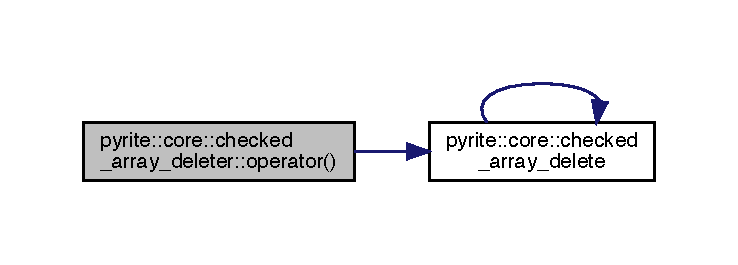
\includegraphics[width=350pt]{dc/dd4/classpyrite_1_1core_1_1checked__array__deleter_a9ac9321cdd986f83350ab5707f9ed4b4_cgraph}
\end{center}
\end{figure}


The documentation for this class was generated from the following file\+:\begin{DoxyCompactItemize}
\item 
/\+Users/masato.\+tanaka/\+Development/cpp/pyrite/pyrite/core/\mbox{\hyperlink{checked__delete_8hpp}{checked\+\_\+delete.\+hpp}}\end{DoxyCompactItemize}

\hypertarget{classpyrite_1_1core_1_1checked__deleter}{}\section{pyrite\+:\+:core\+:\+:checked\+\_\+deleter$<$ T $>$ Class Template Reference}
\label{classpyrite_1_1core_1_1checked__deleter}\index{pyrite\+::core\+::checked\+\_\+deleter$<$ T $>$@{pyrite\+::core\+::checked\+\_\+deleter$<$ T $>$}}


{\ttfamily \#include $<$checked\+\_\+delete.\+hpp$>$}

\subsection*{Public Types}
\begin{DoxyCompactItemize}
\item 
\mbox{\Hypertarget{classpyrite_1_1core_1_1checked__deleter_a9b4af33bca1305708dfa58ce7b42091a}\label{classpyrite_1_1core_1_1checked__deleter_a9b4af33bca1305708dfa58ce7b42091a}} 
using \mbox{\hyperlink{classpyrite_1_1core_1_1checked__deleter_a9b4af33bca1305708dfa58ce7b42091a}{result\+\_\+type}} = void
\begin{DoxyCompactList}\small\item\em The result type of the operator(). \end{DoxyCompactList}\item 
\mbox{\Hypertarget{classpyrite_1_1core_1_1checked__deleter_a98bbd81bf7af52f5595955fccc79433a}\label{classpyrite_1_1core_1_1checked__deleter_a98bbd81bf7af52f5595955fccc79433a}} 
using \mbox{\hyperlink{classpyrite_1_1core_1_1checked__deleter_a98bbd81bf7af52f5595955fccc79433a}{argument\+\_\+type}} = T $\ast$\&
\begin{DoxyCompactList}\small\item\em The argument type of the operator(). \end{DoxyCompactList}\end{DoxyCompactItemize}
\subsection*{Public Member Functions}
\begin{DoxyCompactItemize}
\item 
void \mbox{\hyperlink{classpyrite_1_1core_1_1checked__deleter_a214d518516d6f75bb36b941e4f345f6d}{operator()}} (T $\ast$\&ptr) const
\end{DoxyCompactItemize}


\subsection{Detailed Description}
\subsubsection*{template$<$typename T$>$\newline
class pyrite\+::core\+::checked\+\_\+deleter$<$ T $>$}

A function object thet calls checked\+\_\+delete with operator(). 
\begin{DoxyTemplParams}{Template Parameters}
{\em T} & Must be a complete type. \\
\hline
\end{DoxyTemplParams}


\subsection{Member Function Documentation}
\mbox{\Hypertarget{classpyrite_1_1core_1_1checked__deleter_a214d518516d6f75bb36b941e4f345f6d}\label{classpyrite_1_1core_1_1checked__deleter_a214d518516d6f75bb36b941e4f345f6d}} 
\index{pyrite\+::core\+::checked\+\_\+deleter@{pyrite\+::core\+::checked\+\_\+deleter}!operator()@{operator()}}
\index{operator()@{operator()}!pyrite\+::core\+::checked\+\_\+deleter@{pyrite\+::core\+::checked\+\_\+deleter}}
\subsubsection{\texorpdfstring{operator()()}{operator()()}}
{\footnotesize\ttfamily template$<$typename T $>$ \\
void \mbox{\hyperlink{classpyrite_1_1core_1_1checked__deleter}{pyrite\+::core\+::checked\+\_\+deleter}}$<$ T $>$\+::operator() (\begin{DoxyParamCaption}\item[{T $\ast$\&}]{ptr }\end{DoxyParamCaption}) const\hspace{0.3cm}{\ttfamily [inline]}}

Call checked\+\_\+delete. 
\begin{DoxyParams}{Parameters}
{\em ptr} & pointer. \\
\hline
\end{DoxyParams}
Here is the call graph for this function\+:
\nopagebreak
\begin{figure}[H]
\begin{center}
\leavevmode
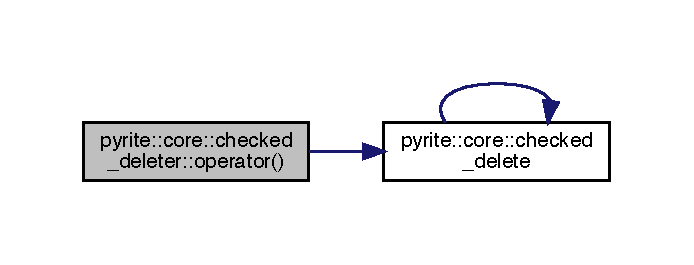
\includegraphics[width=333pt]{dc/d24/classpyrite_1_1core_1_1checked__deleter_a214d518516d6f75bb36b941e4f345f6d_cgraph}
\end{center}
\end{figure}


The documentation for this class was generated from the following file\+:\begin{DoxyCompactItemize}
\item 
/\+Users/masato.\+tanaka/\+Development/cpp/pyrite/pyrite/core/\mbox{\hyperlink{checked__delete_8hpp}{checked\+\_\+delete.\+hpp}}\end{DoxyCompactItemize}

\hypertarget{structpyrite_1_1math_1_1degree__angle__tag__t}{}\section{pyrite\+:\+:math\+:\+:degree\+\_\+angle\+\_\+tag\+\_\+t Struct Reference}
\label{structpyrite_1_1math_1_1degree__angle__tag__t}\index{pyrite\+::math\+::degree\+\_\+angle\+\_\+tag\+\_\+t@{pyrite\+::math\+::degree\+\_\+angle\+\_\+tag\+\_\+t}}


The documentation for this struct was generated from the following file\+:\begin{DoxyCompactItemize}
\item 
/\+Users/masato.\+tanaka/\+Development/cpp/pyrite/pyrite/math/\mbox{\hyperlink{angle_8hpp}{angle.\+hpp}}\end{DoxyCompactItemize}

\hypertarget{structpyrite_1_1core_1_1mpl_1_1filter}{}\section{pyrite\+:\+:core\+:\+:mpl\+:\+:filter$<$ List, F $>$ Struct Template Reference}
\label{structpyrite_1_1core_1_1mpl_1_1filter}\index{pyrite\+::core\+::mpl\+::filter$<$ List, F $>$@{pyrite\+::core\+::mpl\+::filter$<$ List, F $>$}}


The documentation for this struct was generated from the following file\+:\begin{DoxyCompactItemize}
\item 
/\+Users/masato.\+tanaka/\+Development/cpp/pyrite/pyrite/core/mpl/type\+\_\+list/\mbox{\hyperlink{core_2mpl_2type__list_2filter_8hpp}{filter.\+hpp}}\end{DoxyCompactItemize}

\hypertarget{structpyrite_1_1core_1_1mpl_1_1filter_3_01type__list_3_01_args_8_8_8_01_4_00_01_f_01_4}{}\section{pyrite\+:\+:core\+:\+:mpl\+:\+:filter$<$ type\+\_\+list$<$ Args... $>$, F $>$ Struct Template Reference}
\label{structpyrite_1_1core_1_1mpl_1_1filter_3_01type__list_3_01_args_8_8_8_01_4_00_01_f_01_4}\index{pyrite\+::core\+::mpl\+::filter$<$ type\+\_\+list$<$ Args... $>$, F $>$@{pyrite\+::core\+::mpl\+::filter$<$ type\+\_\+list$<$ Args... $>$, F $>$}}
\subsection*{Public Types}
\begin{DoxyCompactItemize}
\item 
\mbox{\Hypertarget{structpyrite_1_1core_1_1mpl_1_1filter_3_01type__list_3_01_args_8_8_8_01_4_00_01_f_01_4_adeba210487d17d017f01d39027f9c1a4}\label{structpyrite_1_1core_1_1mpl_1_1filter_3_01type__list_3_01_args_8_8_8_01_4_00_01_f_01_4_adeba210487d17d017f01d39027f9c1a4}} 
using {\bfseries type} = decltype(apply())
\end{DoxyCompactItemize}


The documentation for this struct was generated from the following file\+:\begin{DoxyCompactItemize}
\item 
/\+Users/masato.\+tanaka/\+Development/cpp/pyrite/pyrite/core/mpl/type\+\_\+list/\mbox{\hyperlink{core_2mpl_2type__list_2filter_8hpp}{filter.\+hpp}}\end{DoxyCompactItemize}

\hypertarget{structpyrite_1_1core_1_1mpl_1_1find__if}{}\section{pyrite\+:\+:core\+:\+:mpl\+:\+:find\+\_\+if$<$ List, F $>$ Struct Template Reference}
\label{structpyrite_1_1core_1_1mpl_1_1find__if}\index{pyrite\+::core\+::mpl\+::find\+\_\+if$<$ List, F $>$@{pyrite\+::core\+::mpl\+::find\+\_\+if$<$ List, F $>$}}
\subsection*{Public Types}
\begin{DoxyCompactItemize}
\item 
\mbox{\Hypertarget{structpyrite_1_1core_1_1mpl_1_1find__if_ae1373592277cc645482016f822963d12}\label{structpyrite_1_1core_1_1mpl_1_1find__if_ae1373592277cc645482016f822963d12}} 
using {\bfseries type} = head\+\_\+t$<$ filter\+\_\+t$<$ List, F $>$ $>$
\end{DoxyCompactItemize}


The documentation for this struct was generated from the following file\+:\begin{DoxyCompactItemize}
\item 
/\+Users/masato.\+tanaka/\+Development/cpp/pyrite/pyrite/core/mpl/type\+\_\+list/\mbox{\hyperlink{core_2mpl_2type__list_2find__if_8hpp}{find\+\_\+if.\+hpp}}\end{DoxyCompactItemize}

\hypertarget{structpyrite_1_1core_1_1mpl_1_1head}{}\section{pyrite\+:\+:core\+:\+:mpl\+:\+:head$<$ T $>$ Struct Template Reference}
\label{structpyrite_1_1core_1_1mpl_1_1head}\index{pyrite\+::core\+::mpl\+::head$<$ T $>$@{pyrite\+::core\+::mpl\+::head$<$ T $>$}}
\subsection*{Public Types}
\begin{DoxyCompactItemize}
\item 
\mbox{\Hypertarget{structpyrite_1_1core_1_1mpl_1_1head_a4fb0efff071569af23d9d0da6506e5fa}\label{structpyrite_1_1core_1_1mpl_1_1head_a4fb0efff071569af23d9d0da6506e5fa}} 
using {\bfseries type} = \mbox{\hyperlink{structpyrite_1_1core_1_1mpl_1_1type__optional_3_4}{null\+\_\+type\+\_\+optional}}
\end{DoxyCompactItemize}


The documentation for this struct was generated from the following file\+:\begin{DoxyCompactItemize}
\item 
/\+Users/masato.\+tanaka/\+Development/cpp/pyrite/pyrite/core/mpl/type\+\_\+list/\mbox{\hyperlink{core_2mpl_2type__list_2head_8hpp}{head.\+hpp}}\end{DoxyCompactItemize}

\hypertarget{structpyrite_1_1core_1_1mpl_1_1head_3_01type__list_3_01_head_00_01_tail_8_8_8_01_4_01_4}{}\section{pyrite\+:\+:core\+:\+:mpl\+:\+:head$<$ type\+\_\+list$<$ Head, Tail... $>$ $>$ Struct Template Reference}
\label{structpyrite_1_1core_1_1mpl_1_1head_3_01type__list_3_01_head_00_01_tail_8_8_8_01_4_01_4}\index{pyrite\+::core\+::mpl\+::head$<$ type\+\_\+list$<$ Head, Tail... $>$ $>$@{pyrite\+::core\+::mpl\+::head$<$ type\+\_\+list$<$ Head, Tail... $>$ $>$}}
\subsection*{Public Types}
\begin{DoxyCompactItemize}
\item 
\mbox{\Hypertarget{structpyrite_1_1core_1_1mpl_1_1head_3_01type__list_3_01_head_00_01_tail_8_8_8_01_4_01_4_a8f35fada089de528196ad3a16b9c978b}\label{structpyrite_1_1core_1_1mpl_1_1head_3_01type__list_3_01_head_00_01_tail_8_8_8_01_4_01_4_a8f35fada089de528196ad3a16b9c978b}} 
using {\bfseries type} = \mbox{\hyperlink{structpyrite_1_1core_1_1mpl_1_1type__optional}{type\+\_\+optional}}$<$ Head $>$
\end{DoxyCompactItemize}


The documentation for this struct was generated from the following file\+:\begin{DoxyCompactItemize}
\item 
/\+Users/masato.\+tanaka/\+Development/cpp/pyrite/pyrite/core/mpl/type\+\_\+list/\mbox{\hyperlink{core_2mpl_2type__list_2head_8hpp}{head.\+hpp}}\end{DoxyCompactItemize}

\hypertarget{classpyrite_1_1core_1_1is__complete__type}{}\section{pyrite\+:\+:core\+:\+:is\+\_\+complete\+\_\+type$<$ T, typename $>$ Class Template Reference}
\label{classpyrite_1_1core_1_1is__complete__type}\index{pyrite\+::core\+::is\+\_\+complete\+\_\+type$<$ T, typename $>$@{pyrite\+::core\+::is\+\_\+complete\+\_\+type$<$ T, typename $>$}}


{\ttfamily \#include $<$is\+\_\+complete\+\_\+type.\+hpp$>$}



Inheritance diagram for pyrite\+:\+:core\+:\+:is\+\_\+complete\+\_\+type$<$ T, typename $>$\+:
\nopagebreak
\begin{figure}[H]
\begin{center}
\leavevmode
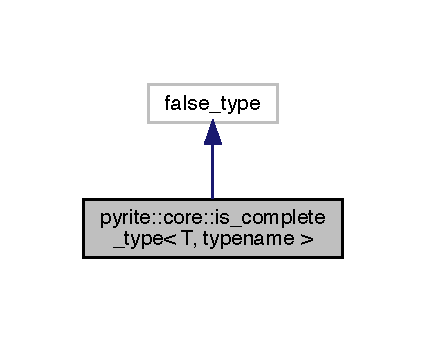
\includegraphics[width=204pt]{dc/d58/classpyrite_1_1core_1_1is__complete__type__inherit__graph}
\end{center}
\end{figure}


Collaboration diagram for pyrite\+:\+:core\+:\+:is\+\_\+complete\+\_\+type$<$ T, typename $>$\+:
\nopagebreak
\begin{figure}[H]
\begin{center}
\leavevmode
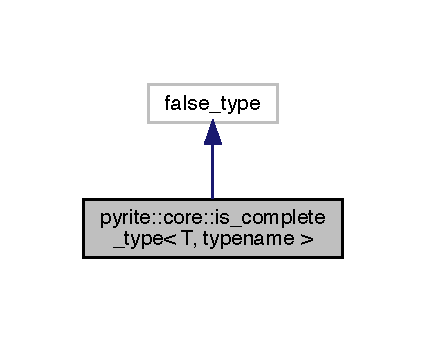
\includegraphics[width=204pt]{db/dc7/classpyrite_1_1core_1_1is__complete__type__coll__graph}
\end{center}
\end{figure}


\subsection{Detailed Description}
\subsubsection*{template$<$typename T, typename = void$>$\newline
class pyrite\+::core\+::is\+\_\+complete\+\_\+type$<$ T, typename $>$}

Checks whether T is an complete type. 
\begin{DoxyTemplParams}{Template Parameters}
{\em T} & A type to check. \\
\hline
\end{DoxyTemplParams}


The documentation for this class was generated from the following file\+:\begin{DoxyCompactItemize}
\item 
/\+Users/masato.\+tanaka/\+Development/cpp/pyrite/pyrite/core/\mbox{\hyperlink{core_2is__complete__type_8hpp}{is\+\_\+complete\+\_\+type.\+hpp}}\end{DoxyCompactItemize}

\hypertarget{classpyrite_1_1core_1_1is__complete__type_3_01_t_00_01std_1_1void__t_3_01decltype_07sizeof_07_t_08_08_4_01_4}{}\section{pyrite\+:\+:core\+:\+:is\+\_\+complete\+\_\+type$<$ T, std\+:\+:void\+\_\+t$<$ decltype(sizeof(T))$>$ $>$ Class Template Reference}
\label{classpyrite_1_1core_1_1is__complete__type_3_01_t_00_01std_1_1void__t_3_01decltype_07sizeof_07_t_08_08_4_01_4}\index{pyrite\+::core\+::is\+\_\+complete\+\_\+type$<$ T, std\+::void\+\_\+t$<$ decltype(sizeof(\+T))$>$ $>$@{pyrite\+::core\+::is\+\_\+complete\+\_\+type$<$ T, std\+::void\+\_\+t$<$ decltype(sizeof(\+T))$>$ $>$}}


{\ttfamily \#include $<$is\+\_\+complete\+\_\+type.\+hpp$>$}



Inheritance diagram for pyrite\+:\+:core\+:\+:is\+\_\+complete\+\_\+type$<$ T, std\+:\+:void\+\_\+t$<$ decltype(sizeof(T))$>$ $>$\+:
\nopagebreak
\begin{figure}[H]
\begin{center}
\leavevmode
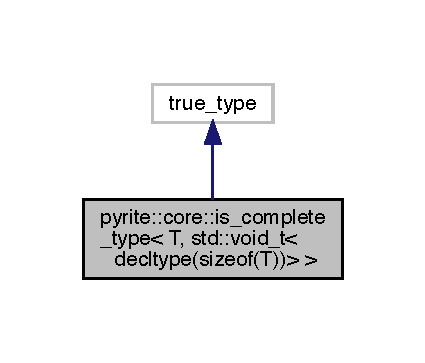
\includegraphics[width=204pt]{df/dae/classpyrite_1_1core_1_1is__complete__type_3_01_t_00_01std_1_1void__t_3_01decltype_07sizeof_07_t_08_08_4_01_4__inherit__graph}
\end{center}
\end{figure}


Collaboration diagram for pyrite\+:\+:core\+:\+:is\+\_\+complete\+\_\+type$<$ T, std\+:\+:void\+\_\+t$<$ decltype(sizeof(T))$>$ $>$\+:
\nopagebreak
\begin{figure}[H]
\begin{center}
\leavevmode
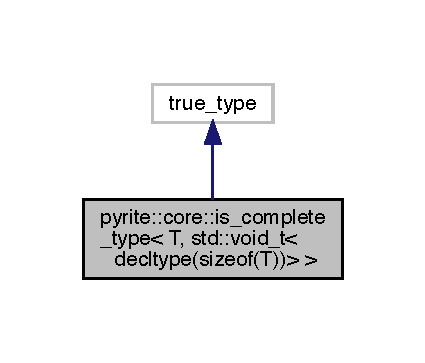
\includegraphics[width=204pt]{da/d64/classpyrite_1_1core_1_1is__complete__type_3_01_t_00_01std_1_1void__t_3_01decltype_07sizeof_07_t_08_08_4_01_4__coll__graph}
\end{center}
\end{figure}


\subsection{Detailed Description}
\subsubsection*{template$<$typename T$>$\newline
class pyrite\+::core\+::is\+\_\+complete\+\_\+type$<$ T, std\+::void\+\_\+t$<$ decltype(sizeof(\+T))$>$ $>$}

Template specialization when T is complete type. 

The documentation for this class was generated from the following file\+:\begin{DoxyCompactItemize}
\item 
/\+Users/masato.\+tanaka/\+Development/cpp/pyrite/pyrite/core/\mbox{\hyperlink{core_2is__complete__type_8hpp}{is\+\_\+complete\+\_\+type.\+hpp}}\end{DoxyCompactItemize}

\hypertarget{structpyrite_1_1type__traits_1_1is__equality__comparable}{}\section{pyrite\+:\+:type\+\_\+traits\+:\+:is\+\_\+equality\+\_\+comparable$<$ T, U, typename $>$ Struct Template Reference}
\label{structpyrite_1_1type__traits_1_1is__equality__comparable}\index{pyrite\+::type\+\_\+traits\+::is\+\_\+equality\+\_\+comparable$<$ T, U, typename $>$@{pyrite\+::type\+\_\+traits\+::is\+\_\+equality\+\_\+comparable$<$ T, U, typename $>$}}


{\ttfamily \#include $<$is\+\_\+equality\+\_\+comparable.\+hpp$>$}



Inheritance diagram for pyrite\+:\+:type\+\_\+traits\+:\+:is\+\_\+equality\+\_\+comparable$<$ T, U, typename $>$\+:
\nopagebreak
\begin{figure}[H]
\begin{center}
\leavevmode
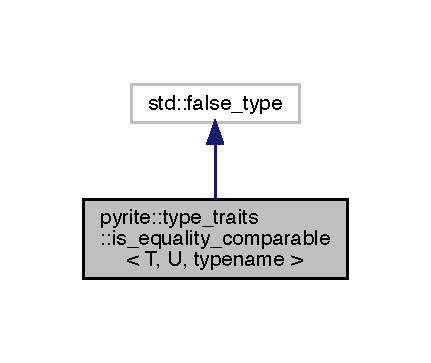
\includegraphics[width=207pt]{d1/da5/structpyrite_1_1type__traits_1_1is__equality__comparable__inherit__graph}
\end{center}
\end{figure}


Collaboration diagram for pyrite\+:\+:type\+\_\+traits\+:\+:is\+\_\+equality\+\_\+comparable$<$ T, U, typename $>$\+:
\nopagebreak
\begin{figure}[H]
\begin{center}
\leavevmode
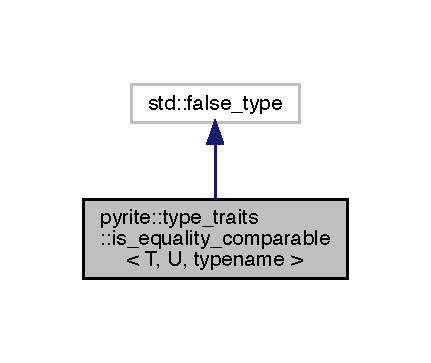
\includegraphics[width=207pt]{db/d38/structpyrite_1_1type__traits_1_1is__equality__comparable__coll__graph}
\end{center}
\end{figure}


\subsection{Detailed Description}
\subsubsection*{template$<$typename T, typename U, typename = void$>$\newline
struct pyrite\+::type\+\_\+traits\+::is\+\_\+equality\+\_\+comparable$<$ T, U, typename $>$}

Whether T and U can be compared with operator==. 
\begin{DoxyTemplParams}{Template Parameters}
{\em T} & Left Type. \\
\hline
{\em U} & Right Type. \\
\hline
\end{DoxyTemplParams}


The documentation for this struct was generated from the following file\+:\begin{DoxyCompactItemize}
\item 
/\+Users/masato.\+tanaka/\+Development/cpp/pyrite/pyrite/type\+\_\+traits/\mbox{\hyperlink{is__equality__comparable_8hpp}{is\+\_\+equality\+\_\+comparable.\+hpp}}\end{DoxyCompactItemize}

\hypertarget{structpyrite_1_1type__traits_1_1is__equality__comparable_3_01_t_00_01_u_00_01std_1_1void__t_3_01fc9a5013d4b968e0ba738bd33a1d5ac1}{}\section{pyrite\+:\+:type\+\_\+traits\+:\+:is\+\_\+equality\+\_\+comparable$<$ T, U, std\+:\+:void\+\_\+t$<$ decltype(std\+:\+:declval$<$ T \& $>$()==std\+:\+:declval$<$ U \& $>$())$>$ $>$ Struct Template Reference}
\label{structpyrite_1_1type__traits_1_1is__equality__comparable_3_01_t_00_01_u_00_01std_1_1void__t_3_01fc9a5013d4b968e0ba738bd33a1d5ac1}\index{pyrite\+::type\+\_\+traits\+::is\+\_\+equality\+\_\+comparable$<$ T, U, std\+::void\+\_\+t$<$ decltype(std\+::declval$<$ T \& $>$()==std\+::declval$<$ U \& $>$())$>$ $>$@{pyrite\+::type\+\_\+traits\+::is\+\_\+equality\+\_\+comparable$<$ T, U, std\+::void\+\_\+t$<$ decltype(std\+::declval$<$ T \& $>$()==std\+::declval$<$ U \& $>$())$>$ $>$}}


{\ttfamily \#include $<$is\+\_\+equality\+\_\+comparable.\+hpp$>$}



Inheritance diagram for pyrite\+:\+:type\+\_\+traits\+:\+:is\+\_\+equality\+\_\+comparable$<$ T, U, std\+:\+:void\+\_\+t$<$ decltype(std\+:\+:declval$<$ T \& $>$()==std\+:\+:declval$<$ U \& $>$())$>$ $>$\+:
\nopagebreak
\begin{figure}[H]
\begin{center}
\leavevmode
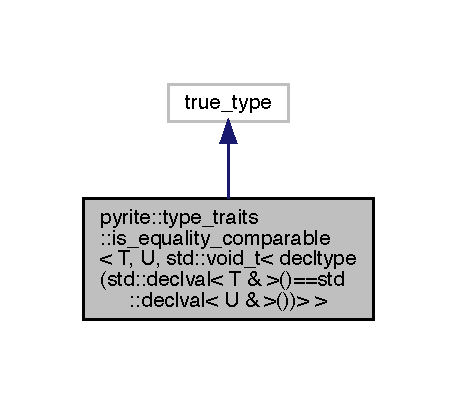
\includegraphics[width=219pt]{d5/d68/structpyrite_1_1type__traits_1_1is__equality__comparable_3_01_t_00_01_u_00_01std_1_1void__t_3_01f9de9051a5d07ee87f867fb2d84341aa}
\end{center}
\end{figure}


Collaboration diagram for pyrite\+:\+:type\+\_\+traits\+:\+:is\+\_\+equality\+\_\+comparable$<$ T, U, std\+:\+:void\+\_\+t$<$ decltype(std\+:\+:declval$<$ T \& $>$()==std\+:\+:declval$<$ U \& $>$())$>$ $>$\+:
\nopagebreak
\begin{figure}[H]
\begin{center}
\leavevmode
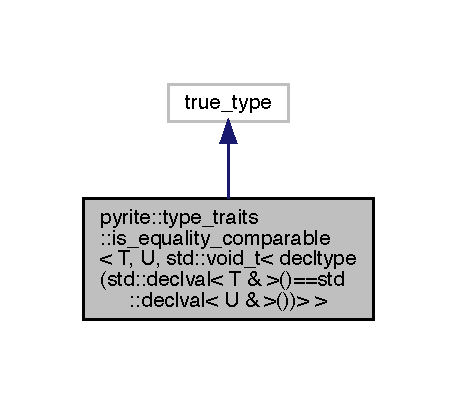
\includegraphics[width=219pt]{dd/d31/structpyrite_1_1type__traits_1_1is__equality__comparable_3_01_t_00_01_u_00_01std_1_1void__t_3_01a799a9b256cbefbf5e3e39d0519e17bf}
\end{center}
\end{figure}


\subsection{Detailed Description}
\subsubsection*{template$<$typename T, typename U$>$\newline
struct pyrite\+::type\+\_\+traits\+::is\+\_\+equality\+\_\+comparable$<$ T, U, std\+::void\+\_\+t$<$ decltype(std\+::declval$<$ T \& $>$()==std\+::declval$<$ U \& $>$())$>$ $>$}

Template specialization when T and U can be compared with operator==. 

The documentation for this struct was generated from the following file\+:\begin{DoxyCompactItemize}
\item 
/\+Users/masato.\+tanaka/\+Development/cpp/pyrite/pyrite/type\+\_\+traits/\mbox{\hyperlink{is__equality__comparable_8hpp}{is\+\_\+equality\+\_\+comparable.\+hpp}}\end{DoxyCompactItemize}

\hypertarget{structpyrite_1_1mpl_1_1at___1_1is__index__of}{}\section{pyrite\+:\+:mpl\+:\+:at\+\_\+\+:\+:is\+\_\+index\+\_\+of$<$ Pair, Index $>$ Struct Template Reference}
\label{structpyrite_1_1mpl_1_1at___1_1is__index__of}\index{pyrite\+::mpl\+::at\+\_\+\+::is\+\_\+index\+\_\+of$<$ Pair, Index $>$@{pyrite\+::mpl\+::at\+\_\+\+::is\+\_\+index\+\_\+of$<$ Pair, Index $>$}}


Inheritance diagram for pyrite\+:\+:mpl\+:\+:at\+\_\+\+:\+:is\+\_\+index\+\_\+of$<$ Pair, Index $>$\+:
\nopagebreak
\begin{figure}[H]
\begin{center}
\leavevmode
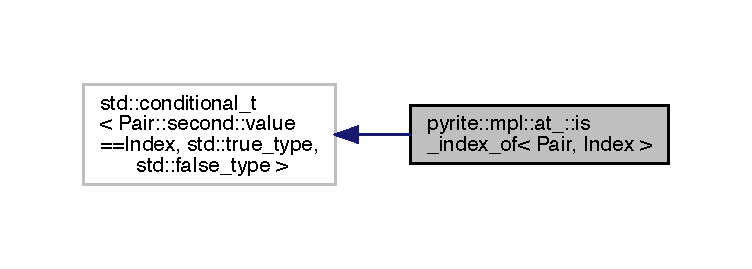
\includegraphics[width=350pt]{dd/d8e/structpyrite_1_1mpl_1_1at___1_1is__index__of__inherit__graph}
\end{center}
\end{figure}


Collaboration diagram for pyrite\+:\+:mpl\+:\+:at\+\_\+\+:\+:is\+\_\+index\+\_\+of$<$ Pair, Index $>$\+:
\nopagebreak
\begin{figure}[H]
\begin{center}
\leavevmode
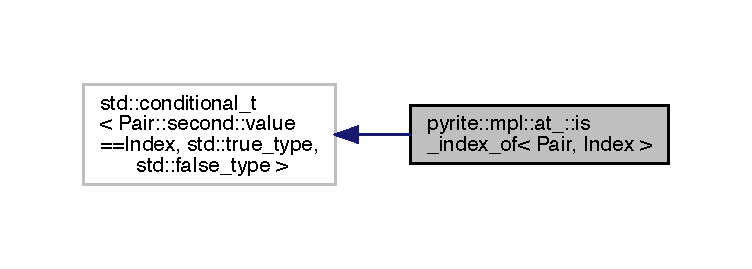
\includegraphics[width=350pt]{db/d7d/structpyrite_1_1mpl_1_1at___1_1is__index__of__coll__graph}
\end{center}
\end{figure}


The documentation for this struct was generated from the following file\+:\begin{DoxyCompactItemize}
\item 
/\+Users/masato.\+tanaka/\+Development/cpp/pyrite/pyrite/mpl/type\+\_\+list/\mbox{\hyperlink{at_8hpp}{at.\+hpp}}\end{DoxyCompactItemize}

\hypertarget{structpyrite_1_1core_1_1mpl_1_1is__type__list}{}\section{pyrite\+:\+:core\+:\+:mpl\+:\+:is\+\_\+type\+\_\+list$<$ T $>$ Struct Template Reference}
\label{structpyrite_1_1core_1_1mpl_1_1is__type__list}\index{pyrite\+::core\+::mpl\+::is\+\_\+type\+\_\+list$<$ T $>$@{pyrite\+::core\+::mpl\+::is\+\_\+type\+\_\+list$<$ T $>$}}


Inheritance diagram for pyrite\+:\+:core\+:\+:mpl\+:\+:is\+\_\+type\+\_\+list$<$ T $>$\+:
\nopagebreak
\begin{figure}[H]
\begin{center}
\leavevmode
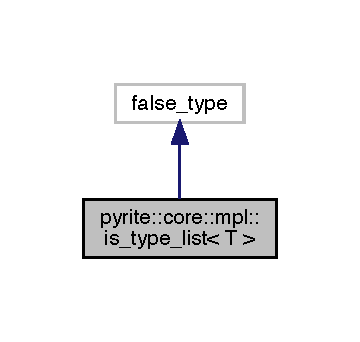
\includegraphics[width=173pt]{dd/dbf/structpyrite_1_1core_1_1mpl_1_1is__type__list__inherit__graph}
\end{center}
\end{figure}


Collaboration diagram for pyrite\+:\+:core\+:\+:mpl\+:\+:is\+\_\+type\+\_\+list$<$ T $>$\+:
\nopagebreak
\begin{figure}[H]
\begin{center}
\leavevmode
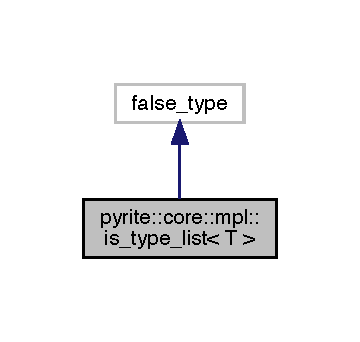
\includegraphics[width=173pt]{de/d37/structpyrite_1_1core_1_1mpl_1_1is__type__list__coll__graph}
\end{center}
\end{figure}


The documentation for this struct was generated from the following file\+:\begin{DoxyCompactItemize}
\item 
/\+Users/masato.\+tanaka/\+Development/cpp/pyrite/pyrite/core/mpl/type\+\_\+list/\mbox{\hyperlink{core_2mpl_2type__list_2is__type__list_8hpp}{is\+\_\+type\+\_\+list.\+hpp}}\end{DoxyCompactItemize}

\hypertarget{structpyrite_1_1core_1_1mpl_1_1is__type__list_3_01type__list_3_01_args_8_8_8_01_4_01_4}{}\section{pyrite\+:\+:core\+:\+:mpl\+:\+:is\+\_\+type\+\_\+list$<$ type\+\_\+list$<$ Args... $>$ $>$ Struct Template Reference}
\label{structpyrite_1_1core_1_1mpl_1_1is__type__list_3_01type__list_3_01_args_8_8_8_01_4_01_4}\index{pyrite\+::core\+::mpl\+::is\+\_\+type\+\_\+list$<$ type\+\_\+list$<$ Args... $>$ $>$@{pyrite\+::core\+::mpl\+::is\+\_\+type\+\_\+list$<$ type\+\_\+list$<$ Args... $>$ $>$}}


Inheritance diagram for pyrite\+:\+:core\+:\+:mpl\+:\+:is\+\_\+type\+\_\+list$<$ type\+\_\+list$<$ Args... $>$ $>$\+:
\nopagebreak
\begin{figure}[H]
\begin{center}
\leavevmode
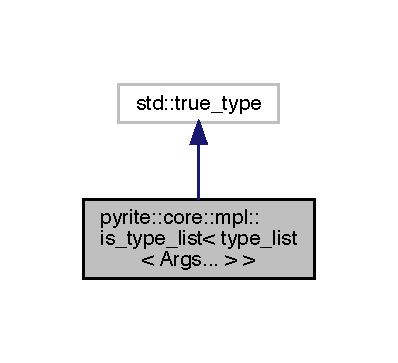
\includegraphics[width=191pt]{d9/dc3/structpyrite_1_1core_1_1mpl_1_1is__type__list_3_01type__list_3_01_args_8_8_8_01_4_01_4__inherit__graph}
\end{center}
\end{figure}


Collaboration diagram for pyrite\+:\+:core\+:\+:mpl\+:\+:is\+\_\+type\+\_\+list$<$ type\+\_\+list$<$ Args... $>$ $>$\+:
\nopagebreak
\begin{figure}[H]
\begin{center}
\leavevmode
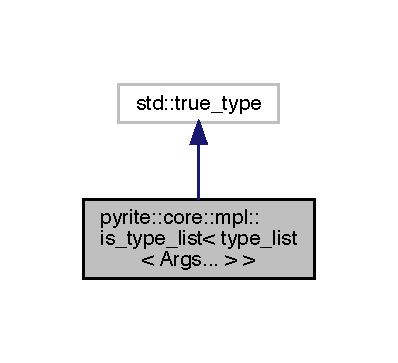
\includegraphics[width=191pt]{de/d80/structpyrite_1_1core_1_1mpl_1_1is__type__list_3_01type__list_3_01_args_8_8_8_01_4_01_4__coll__graph}
\end{center}
\end{figure}


The documentation for this struct was generated from the following file\+:\begin{DoxyCompactItemize}
\item 
/\+Users/masato.\+tanaka/\+Development/cpp/pyrite/pyrite/core/mpl/type\+\_\+list/\mbox{\hyperlink{core_2mpl_2type__list_2is__type__list_8hpp}{is\+\_\+type\+\_\+list.\+hpp}}\end{DoxyCompactItemize}

\hypertarget{structpyrite_1_1mpl_1_1join}{}\section{pyrite\+:\+:mpl\+:\+:join$<$ ListL, ListR $>$ Struct Template Reference}
\label{structpyrite_1_1mpl_1_1join}\index{pyrite\+::mpl\+::join$<$ List\+L, List\+R $>$@{pyrite\+::mpl\+::join$<$ List\+L, List\+R $>$}}


The documentation for this struct was generated from the following file\+:\begin{DoxyCompactItemize}
\item 
/\+Users/masato.\+tanaka/\+Development/cpp/pyrite/pyrite/mpl/type\+\_\+list/\mbox{\hyperlink{join_8hpp}{join.\+hpp}}\end{DoxyCompactItemize}

\hypertarget{structpyrite_1_1mpl_1_1join_3_01type__list_3_01_l_8_8_8_01_4_00_01type__list_3_01_r_8_8_8_01_4_01_4}{}\section{pyrite\+:\+:mpl\+:\+:join$<$ type\+\_\+list$<$ L... $>$, type\+\_\+list$<$ R... $>$ $>$ Struct Template Reference}
\label{structpyrite_1_1mpl_1_1join_3_01type__list_3_01_l_8_8_8_01_4_00_01type__list_3_01_r_8_8_8_01_4_01_4}\index{pyrite\+::mpl\+::join$<$ type\+\_\+list$<$ L... $>$, type\+\_\+list$<$ R... $>$ $>$@{pyrite\+::mpl\+::join$<$ type\+\_\+list$<$ L... $>$, type\+\_\+list$<$ R... $>$ $>$}}
\subsection*{Public Types}
\begin{DoxyCompactItemize}
\item 
\mbox{\Hypertarget{structpyrite_1_1mpl_1_1join_3_01type__list_3_01_l_8_8_8_01_4_00_01type__list_3_01_r_8_8_8_01_4_01_4_ac9e74c452c32febc687872c9e413cbe3}\label{structpyrite_1_1mpl_1_1join_3_01type__list_3_01_l_8_8_8_01_4_00_01type__list_3_01_r_8_8_8_01_4_01_4_ac9e74c452c32febc687872c9e413cbe3}} 
using {\bfseries type} = \mbox{\hyperlink{structpyrite_1_1core_1_1mpl_1_1type__list}{type\+\_\+list}}$<$ L..., R... $>$
\end{DoxyCompactItemize}


The documentation for this struct was generated from the following file\+:\begin{DoxyCompactItemize}
\item 
/\+Users/masato.\+tanaka/\+Development/cpp/pyrite/pyrite/mpl/type\+\_\+list/\mbox{\hyperlink{join_8hpp}{join.\+hpp}}\end{DoxyCompactItemize}

\hypertarget{structpyrite_1_1mpl_1_1make__type__list___1_1make__type__list}{}\section{pyrite\+:\+:mpl\+:\+:make\+\_\+type\+\_\+list\+\_\+\+:\+:make\+\_\+type\+\_\+list$<$ T, Size $>$ Struct Template Reference}
\label{structpyrite_1_1mpl_1_1make__type__list___1_1make__type__list}\index{pyrite\+::mpl\+::make\+\_\+type\+\_\+list\+\_\+\+::make\+\_\+type\+\_\+list$<$ T, Size $>$@{pyrite\+::mpl\+::make\+\_\+type\+\_\+list\+\_\+\+::make\+\_\+type\+\_\+list$<$ T, Size $>$}}
\subsection*{Public Types}
\begin{DoxyCompactItemize}
\item 
\mbox{\Hypertarget{structpyrite_1_1mpl_1_1make__type__list___1_1make__type__list_abb4c4527365bf27071ec6f54206bdf34}\label{structpyrite_1_1mpl_1_1make__type__list___1_1make__type__list_abb4c4527365bf27071ec6f54206bdf34}} 
using {\bfseries type} = typename \mbox{\hyperlink{structpyrite_1_1mpl_1_1make__type__list___1_1sequence__to__list}{sequence\+\_\+to\+\_\+list}}$<$ T, sequence $>$\+::type
\end{DoxyCompactItemize}


The documentation for this struct was generated from the following file\+:\begin{DoxyCompactItemize}
\item 
/\+Users/masato.\+tanaka/\+Development/cpp/pyrite/pyrite/mpl/type\+\_\+list/\mbox{\hyperlink{make__type__list_8hpp}{make\+\_\+type\+\_\+list.\+hpp}}\end{DoxyCompactItemize}

\hypertarget{structpyrite_1_1mpl_1_1make__type__list___1_1make__type__list_3_01_t_00_010_01_4}{}\section{pyrite\+:\+:mpl\+:\+:make\+\_\+type\+\_\+list\+\_\+\+:\+:make\+\_\+type\+\_\+list$<$ T, 0 $>$ Struct Template Reference}
\label{structpyrite_1_1mpl_1_1make__type__list___1_1make__type__list_3_01_t_00_010_01_4}\index{pyrite\+::mpl\+::make\+\_\+type\+\_\+list\+\_\+\+::make\+\_\+type\+\_\+list$<$ T, 0 $>$@{pyrite\+::mpl\+::make\+\_\+type\+\_\+list\+\_\+\+::make\+\_\+type\+\_\+list$<$ T, 0 $>$}}
\subsection*{Public Types}
\begin{DoxyCompactItemize}
\item 
\mbox{\Hypertarget{structpyrite_1_1mpl_1_1make__type__list___1_1make__type__list_3_01_t_00_010_01_4_aa8ea8a480094972a2d355db8025fa380}\label{structpyrite_1_1mpl_1_1make__type__list___1_1make__type__list_3_01_t_00_010_01_4_aa8ea8a480094972a2d355db8025fa380}} 
using {\bfseries type} = \mbox{\hyperlink{structpyrite_1_1core_1_1mpl_1_1type__list}{type\+\_\+list}}$<$$>$
\end{DoxyCompactItemize}


The documentation for this struct was generated from the following file\+:\begin{DoxyCompactItemize}
\item 
/\+Users/masato.\+tanaka/\+Development/cpp/pyrite/pyrite/mpl/type\+\_\+list/\mbox{\hyperlink{make__type__list_8hpp}{make\+\_\+type\+\_\+list.\+hpp}}\end{DoxyCompactItemize}

\hypertarget{classpyrite_1_1core_1_1noncopyable___1_1noncopyable}{}\section{pyrite\+:\+:core\+:\+:noncopyable\+\_\+\+:\+:noncopyable Class Reference}
\label{classpyrite_1_1core_1_1noncopyable___1_1noncopyable}\index{pyrite\+::core\+::noncopyable\+\_\+\+::noncopyable@{pyrite\+::core\+::noncopyable\+\_\+\+::noncopyable}}


Inheritance diagram for pyrite\+:\+:core\+:\+:noncopyable\+\_\+\+:\+:noncopyable\+:
\nopagebreak
\begin{figure}[H]
\begin{center}
\leavevmode
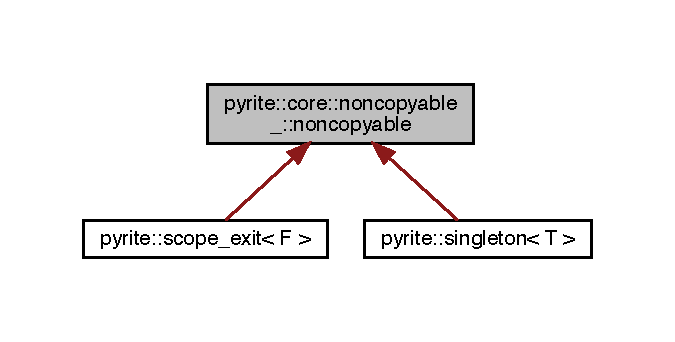
\includegraphics[width=324pt]{df/d64/classpyrite_1_1core_1_1noncopyable___1_1noncopyable__inherit__graph}
\end{center}
\end{figure}
\subsection*{Protected Member Functions}
\begin{DoxyCompactItemize}
\item 
constexpr \mbox{\hyperlink{classpyrite_1_1core_1_1noncopyable___1_1noncopyable_a4a81c76fa6f35c99c55206d61225b34d}{noncopyable}} ()=default
\item 
\mbox{\hyperlink{classpyrite_1_1core_1_1noncopyable___1_1noncopyable_a4c38a4adec1bfca43cbfe5c90c3ee46c}{$\sim$noncopyable}} ()=default
\item 
\mbox{\hyperlink{classpyrite_1_1core_1_1noncopyable___1_1noncopyable_af2fd68ae3feae618e80a6fa92146a962}{noncopyable}} (\mbox{\hyperlink{classpyrite_1_1core_1_1noncopyable___1_1noncopyable}{noncopyable}} const \&)=delete
\item 
\mbox{\hyperlink{classpyrite_1_1core_1_1noncopyable___1_1noncopyable}{noncopyable}} \& \mbox{\hyperlink{classpyrite_1_1core_1_1noncopyable___1_1noncopyable_a6c535716da364f40a0003d85c60d4261}{operator=}} (\mbox{\hyperlink{classpyrite_1_1core_1_1noncopyable___1_1noncopyable}{noncopyable}} const \&)=delete
\end{DoxyCompactItemize}


\subsection{Constructor \& Destructor Documentation}
\mbox{\Hypertarget{classpyrite_1_1core_1_1noncopyable___1_1noncopyable_a4a81c76fa6f35c99c55206d61225b34d}\label{classpyrite_1_1core_1_1noncopyable___1_1noncopyable_a4a81c76fa6f35c99c55206d61225b34d}} 
\index{pyrite\+::core\+::noncopyable\+\_\+\+::noncopyable@{pyrite\+::core\+::noncopyable\+\_\+\+::noncopyable}!noncopyable@{noncopyable}}
\index{noncopyable@{noncopyable}!pyrite\+::core\+::noncopyable\+\_\+\+::noncopyable@{pyrite\+::core\+::noncopyable\+\_\+\+::noncopyable}}
\subsubsection{\texorpdfstring{noncopyable()}{noncopyable()}\hspace{0.1cm}{\footnotesize\ttfamily [1/2]}}
{\footnotesize\ttfamily constexpr pyrite\+::core\+::noncopyable\+\_\+\+::noncopyable\+::noncopyable (\begin{DoxyParamCaption}{ }\end{DoxyParamCaption})\hspace{0.3cm}{\ttfamily [protected]}, {\ttfamily [default]}}

Default constructor. generated by the compiler. \mbox{\Hypertarget{classpyrite_1_1core_1_1noncopyable___1_1noncopyable_a4c38a4adec1bfca43cbfe5c90c3ee46c}\label{classpyrite_1_1core_1_1noncopyable___1_1noncopyable_a4c38a4adec1bfca43cbfe5c90c3ee46c}} 
\index{pyrite\+::core\+::noncopyable\+\_\+\+::noncopyable@{pyrite\+::core\+::noncopyable\+\_\+\+::noncopyable}!````~noncopyable@{$\sim$noncopyable}}
\index{````~noncopyable@{$\sim$noncopyable}!pyrite\+::core\+::noncopyable\+\_\+\+::noncopyable@{pyrite\+::core\+::noncopyable\+\_\+\+::noncopyable}}
\subsubsection{\texorpdfstring{$\sim$noncopyable()}{~noncopyable()}}
{\footnotesize\ttfamily pyrite\+::core\+::noncopyable\+\_\+\+::noncopyable\+::$\sim$noncopyable (\begin{DoxyParamCaption}{ }\end{DoxyParamCaption})\hspace{0.3cm}{\ttfamily [protected]}, {\ttfamily [default]}}

Destructor. generated by the compiler. \mbox{\Hypertarget{classpyrite_1_1core_1_1noncopyable___1_1noncopyable_af2fd68ae3feae618e80a6fa92146a962}\label{classpyrite_1_1core_1_1noncopyable___1_1noncopyable_af2fd68ae3feae618e80a6fa92146a962}} 
\index{pyrite\+::core\+::noncopyable\+\_\+\+::noncopyable@{pyrite\+::core\+::noncopyable\+\_\+\+::noncopyable}!noncopyable@{noncopyable}}
\index{noncopyable@{noncopyable}!pyrite\+::core\+::noncopyable\+\_\+\+::noncopyable@{pyrite\+::core\+::noncopyable\+\_\+\+::noncopyable}}
\subsubsection{\texorpdfstring{noncopyable()}{noncopyable()}\hspace{0.1cm}{\footnotesize\ttfamily [2/2]}}
{\footnotesize\ttfamily pyrite\+::core\+::noncopyable\+\_\+\+::noncopyable\+::noncopyable (\begin{DoxyParamCaption}\item[{\mbox{\hyperlink{classpyrite_1_1core_1_1noncopyable___1_1noncopyable}{noncopyable}} const \&}]{ }\end{DoxyParamCaption})\hspace{0.3cm}{\ttfamily [protected]}, {\ttfamily [delete]}}

Delete copy constructor. 

\subsection{Member Function Documentation}
\mbox{\Hypertarget{classpyrite_1_1core_1_1noncopyable___1_1noncopyable_a6c535716da364f40a0003d85c60d4261}\label{classpyrite_1_1core_1_1noncopyable___1_1noncopyable_a6c535716da364f40a0003d85c60d4261}} 
\index{pyrite\+::core\+::noncopyable\+\_\+\+::noncopyable@{pyrite\+::core\+::noncopyable\+\_\+\+::noncopyable}!operator=@{operator=}}
\index{operator=@{operator=}!pyrite\+::core\+::noncopyable\+\_\+\+::noncopyable@{pyrite\+::core\+::noncopyable\+\_\+\+::noncopyable}}
\subsubsection{\texorpdfstring{operator=()}{operator=()}}
{\footnotesize\ttfamily \mbox{\hyperlink{classpyrite_1_1core_1_1noncopyable___1_1noncopyable}{noncopyable}}\& pyrite\+::core\+::noncopyable\+\_\+\+::noncopyable\+::operator= (\begin{DoxyParamCaption}\item[{\mbox{\hyperlink{classpyrite_1_1core_1_1noncopyable___1_1noncopyable}{noncopyable}} const \&}]{ }\end{DoxyParamCaption})\hspace{0.3cm}{\ttfamily [protected]}, {\ttfamily [delete]}}

Delete copy assignment operator. 

The documentation for this class was generated from the following file\+:\begin{DoxyCompactItemize}
\item 
/\+Users/masato.\+tanaka/\+Development/cpp/pyrite/pyrite/core/\mbox{\hyperlink{noncopyable_8hpp}{noncopyable.\+hpp}}\end{DoxyCompactItemize}

\hypertarget{structpyrite_1_1mpl_1_1none__of}{}\section{pyrite\+:\+:mpl\+:\+:none\+\_\+of$<$ List, F $>$ Struct Template Reference}
\label{structpyrite_1_1mpl_1_1none__of}\index{pyrite\+::mpl\+::none\+\_\+of$<$ List, F $>$@{pyrite\+::mpl\+::none\+\_\+of$<$ List, F $>$}}


Inheritance diagram for pyrite\+:\+:mpl\+:\+:none\+\_\+of$<$ List, F $>$\+:
\nopagebreak
\begin{figure}[H]
\begin{center}
\leavevmode
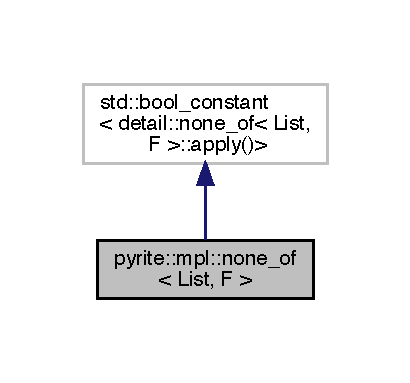
\includegraphics[width=197pt]{d6/d4d/structpyrite_1_1mpl_1_1none__of__inherit__graph}
\end{center}
\end{figure}


Collaboration diagram for pyrite\+:\+:mpl\+:\+:none\+\_\+of$<$ List, F $>$\+:
\nopagebreak
\begin{figure}[H]
\begin{center}
\leavevmode
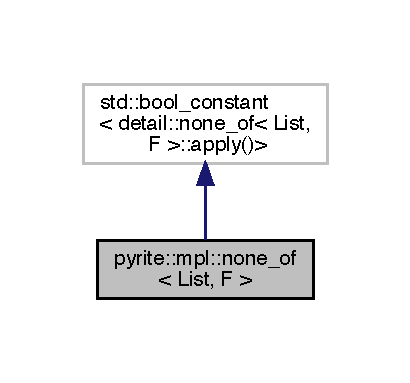
\includegraphics[width=197pt]{d6/d55/structpyrite_1_1mpl_1_1none__of__coll__graph}
\end{center}
\end{figure}


The documentation for this struct was generated from the following file\+:\begin{DoxyCompactItemize}
\item 
/\+Users/masato.\+tanaka/\+Development/cpp/pyrite/pyrite/mpl/type\+\_\+list/\mbox{\hyperlink{none__of_8hpp}{none\+\_\+of.\+hpp}}\end{DoxyCompactItemize}

\hypertarget{structpyrite_1_1mpl_1_1push__back}{}\section{pyrite\+:\+:mpl\+:\+:push\+\_\+back$<$ List, T $>$ Struct Template Reference}
\label{structpyrite_1_1mpl_1_1push__back}\index{pyrite\+::mpl\+::push\+\_\+back$<$ List, T $>$@{pyrite\+::mpl\+::push\+\_\+back$<$ List, T $>$}}
\subsection*{Public Types}
\begin{DoxyCompactItemize}
\item 
\mbox{\Hypertarget{structpyrite_1_1mpl_1_1push__back_a659337124738a4b3b8f2c03b594c0279}\label{structpyrite_1_1mpl_1_1push__back_a659337124738a4b3b8f2c03b594c0279}} 
using {\bfseries type} = join\+\_\+t$<$ List, \mbox{\hyperlink{structpyrite_1_1core_1_1mpl_1_1type__list}{type\+\_\+list}}$<$ T $>$ $>$
\end{DoxyCompactItemize}


The documentation for this struct was generated from the following file\+:\begin{DoxyCompactItemize}
\item 
/\+Users/masato.\+tanaka/\+Development/cpp/pyrite/pyrite/mpl/type\+\_\+list/\mbox{\hyperlink{push__bach_8hpp}{push\+\_\+bach.\+hpp}}\end{DoxyCompactItemize}

\hypertarget{structpyrite_1_1mpl_1_1push__front}{}\section{pyrite\+:\+:mpl\+:\+:push\+\_\+front$<$ List, T $>$ Struct Template Reference}
\label{structpyrite_1_1mpl_1_1push__front}\index{pyrite\+::mpl\+::push\+\_\+front$<$ List, T $>$@{pyrite\+::mpl\+::push\+\_\+front$<$ List, T $>$}}
\subsection*{Public Types}
\begin{DoxyCompactItemize}
\item 
\mbox{\Hypertarget{structpyrite_1_1mpl_1_1push__front_a5cfea53f49a9f5644336d04c321aef97}\label{structpyrite_1_1mpl_1_1push__front_a5cfea53f49a9f5644336d04c321aef97}} 
using {\bfseries type} = join\+\_\+t$<$ \mbox{\hyperlink{structpyrite_1_1core_1_1mpl_1_1type__list}{type\+\_\+list}}$<$ T $>$, List $>$
\end{DoxyCompactItemize}


The documentation for this struct was generated from the following file\+:\begin{DoxyCompactItemize}
\item 
/\+Users/masato.\+tanaka/\+Development/cpp/pyrite/pyrite/mpl/type\+\_\+list/\mbox{\hyperlink{push__front_8hpp}{push\+\_\+front.\+hpp}}\end{DoxyCompactItemize}

\hypertarget{structpyrite_1_1math_1_1radian__angle__tag__t}{}\section{pyrite\+:\+:math\+:\+:radian\+\_\+angle\+\_\+tag\+\_\+t Struct Reference}
\label{structpyrite_1_1math_1_1radian__angle__tag__t}\index{pyrite\+::math\+::radian\+\_\+angle\+\_\+tag\+\_\+t@{pyrite\+::math\+::radian\+\_\+angle\+\_\+tag\+\_\+t}}


The documentation for this struct was generated from the following file\+:\begin{DoxyCompactItemize}
\item 
/\+Users/masato.\+tanaka/\+Development/cpp/pyrite/pyrite/math/\mbox{\hyperlink{angle_8hpp}{angle.\+hpp}}\end{DoxyCompactItemize}

\hypertarget{classpyrite_1_1random}{}\section{pyrite\+:\+:random Class Reference}
\label{classpyrite_1_1random}\index{pyrite\+::random@{pyrite\+::random}}


{\ttfamily \#include $<$random.\+hpp$>$}

\subsection*{Public Types}
\begin{DoxyCompactItemize}
\item 
using \mbox{\hyperlink{classpyrite_1_1random_a936dc9fd106c9b125ccbf3aa6d525e4b}{seed\+\_\+type}} = decltype(\mbox{\hyperlink{structpyrite_1_1random__state_a0e2c55b67459b8e81c7d94cde7aab26a}{random\+\_\+state\+::seed}})
\end{DoxyCompactItemize}
\subsection*{Public Member Functions}
\begin{DoxyCompactItemize}
\item 
\mbox{\hyperlink{classpyrite_1_1random_ac3e5e10f4dd1474afe856780ba8d71e3}{random}} ()
\item 
\mbox{\hyperlink{classpyrite_1_1random_a593c1826bad1b27d489ee55c85da30b3}{random}} (\mbox{\hyperlink{structpyrite_1_1random__state}{random\+\_\+state}} const \&\mbox{\hyperlink{classpyrite_1_1random_a25c469022ddee73c6a4ecce2814d22d4}{state}})
\item 
\mbox{\hyperlink{classpyrite_1_1random_a9f0f5391be20a8fdc3d6009e14dc0bfe}{random}} (\mbox{\hyperlink{classpyrite_1_1random_a936dc9fd106c9b125ccbf3aa6d525e4b}{seed\+\_\+type}} \mbox{\hyperlink{classpyrite_1_1random_ae3a15129c724af7168f55135226c0dfc}{seed}})
\item 
\mbox{\hyperlink{classpyrite_1_1random_ab3ef314958056708117ab37d2dded013}{random}} (\mbox{\hyperlink{classpyrite_1_1random}{random}} const \&other)
\item 
\mbox{\hyperlink{classpyrite_1_1random_a263c5a878b5aaa150d915d765420f294}{random}} (\mbox{\hyperlink{classpyrite_1_1random}{random}} \&\&other)
\item 
\mbox{\hyperlink{classpyrite_1_1random_ae8d71dcc48a9eb0fe84525b368b91e05}{$\sim$random}} ()=default
\item 
{\footnotesize template$<$typename T $>$ }\\auto \mbox{\hyperlink{classpyrite_1_1random_a708282ad1435ee4b9564c8e11baf43f8}{next}} ()
\item 
{\footnotesize template$<$typename T $>$ }\\auto \mbox{\hyperlink{classpyrite_1_1random_a79e67ec7537ab7e872cb1327dbe0bb3e}{next}} (T const \&min, T const \&max)
\item 
\mbox{\hyperlink{classpyrite_1_1random_a936dc9fd106c9b125ccbf3aa6d525e4b}{seed\+\_\+type}} \mbox{\hyperlink{classpyrite_1_1random_ae3a15129c724af7168f55135226c0dfc}{seed}} () const noexcept
\item 
\mbox{\hyperlink{structpyrite_1_1random__state}{random\+\_\+state}} \mbox{\hyperlink{classpyrite_1_1random_a25c469022ddee73c6a4ecce2814d22d4}{state}} () const noexcept
\item 
void \mbox{\hyperlink{classpyrite_1_1random_a8414030e5c428c20b8a8333542918f8c}{discard}} (\mbox{\hyperlink{type_8hpp_a89cb75b6e56f357c2964bbd5520be899}{u64}} z)
\item 
void \mbox{\hyperlink{classpyrite_1_1random_aed264da4ddd55aab1cf72ddb091ec902}{reset}} ()
\item 
void \mbox{\hyperlink{classpyrite_1_1random_a6d5947d6c425031e81f8488187a332f3}{reset}} (\mbox{\hyperlink{classpyrite_1_1random_a936dc9fd106c9b125ccbf3aa6d525e4b}{seed\+\_\+type}} \mbox{\hyperlink{classpyrite_1_1random_ae3a15129c724af7168f55135226c0dfc}{seed}})
\item 
void \mbox{\hyperlink{classpyrite_1_1random_a5abed1bb1fbd44ea3e62197a9b11dcd0}{reset}} (\mbox{\hyperlink{structpyrite_1_1random__state}{random\+\_\+state}} const \&\mbox{\hyperlink{classpyrite_1_1random_a25c469022ddee73c6a4ecce2814d22d4}{state}})
\item 
bool \mbox{\hyperlink{classpyrite_1_1random_a6c58ae19800d0e1f8388b6afbb79a1ba}{operator==}} (\mbox{\hyperlink{classpyrite_1_1random}{random}} const \&rhs) const noexcept
\item 
bool \mbox{\hyperlink{classpyrite_1_1random_aaef2fad3aa9ae947e7ed640db176373e}{operator!=}} (\mbox{\hyperlink{classpyrite_1_1random}{random}} const \&rhs) const noexcept
\item 
\mbox{\hyperlink{classpyrite_1_1random}{random}} \& \mbox{\hyperlink{classpyrite_1_1random_a3cd7cfec2938a1bd9541f34bf2b7ac77}{operator=}} (\mbox{\hyperlink{classpyrite_1_1random}{random}} const \&rhs)
\item 
\mbox{\hyperlink{classpyrite_1_1random}{random}} \& \mbox{\hyperlink{classpyrite_1_1random_a611890eeb411e9081e218d68bb507810}{operator=}} (\mbox{\hyperlink{classpyrite_1_1random}{random}} \&\&rhs)
\end{DoxyCompactItemize}


\subsection{Detailed Description}
Wrapper standard random number generator and distribution generator. 

\subsection{Member Typedef Documentation}
\mbox{\Hypertarget{classpyrite_1_1random_a936dc9fd106c9b125ccbf3aa6d525e4b}\label{classpyrite_1_1random_a936dc9fd106c9b125ccbf3aa6d525e4b}} 
\index{pyrite\+::random@{pyrite\+::random}!seed\+\_\+type@{seed\+\_\+type}}
\index{seed\+\_\+type@{seed\+\_\+type}!pyrite\+::random@{pyrite\+::random}}
\subsubsection{\texorpdfstring{seed\+\_\+type}{seed\_type}}
{\footnotesize\ttfamily using \mbox{\hyperlink{classpyrite_1_1random_a936dc9fd106c9b125ccbf3aa6d525e4b}{pyrite\+::random\+::seed\+\_\+type}} =  decltype(\mbox{\hyperlink{structpyrite_1_1random__state_a0e2c55b67459b8e81c7d94cde7aab26a}{random\+\_\+state\+::seed}})}

Seed type 

\subsection{Constructor \& Destructor Documentation}
\mbox{\Hypertarget{classpyrite_1_1random_ac3e5e10f4dd1474afe856780ba8d71e3}\label{classpyrite_1_1random_ac3e5e10f4dd1474afe856780ba8d71e3}} 
\index{pyrite\+::random@{pyrite\+::random}!random@{random}}
\index{random@{random}!pyrite\+::random@{pyrite\+::random}}
\subsubsection{\texorpdfstring{random()}{random()}\hspace{0.1cm}{\footnotesize\ttfamily [1/5]}}
{\footnotesize\ttfamily pyrite\+::random\+::random (\begin{DoxyParamCaption}{ }\end{DoxyParamCaption})}

Default constructor.

initialized with true random number. \mbox{\Hypertarget{classpyrite_1_1random_a593c1826bad1b27d489ee55c85da30b3}\label{classpyrite_1_1random_a593c1826bad1b27d489ee55c85da30b3}} 
\index{pyrite\+::random@{pyrite\+::random}!random@{random}}
\index{random@{random}!pyrite\+::random@{pyrite\+::random}}
\subsubsection{\texorpdfstring{random()}{random()}\hspace{0.1cm}{\footnotesize\ttfamily [2/5]}}
{\footnotesize\ttfamily pyrite\+::random\+::random (\begin{DoxyParamCaption}\item[{\mbox{\hyperlink{structpyrite_1_1random__state}{random\+\_\+state}} const \&}]{state }\end{DoxyParamCaption})\hspace{0.3cm}{\ttfamily [explicit]}}

Constructor initialized with \mbox{\hyperlink{structpyrite_1_1random__state}{random\+\_\+state}}.


\begin{DoxyParams}[1]{Parameters}
\mbox{\tt in}  & {\em state} & Random\+\_\+state object. \\
\hline
\end{DoxyParams}
Here is the call graph for this function\+:
\nopagebreak
\begin{figure}[H]
\begin{center}
\leavevmode
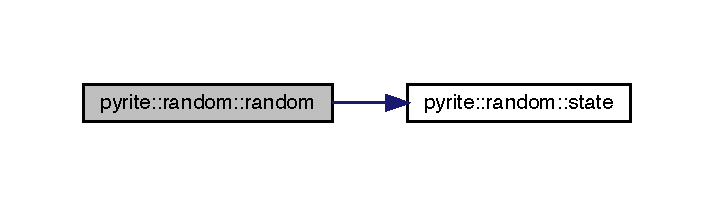
\includegraphics[width=343pt]{d2/df9/classpyrite_1_1random_a593c1826bad1b27d489ee55c85da30b3_cgraph}
\end{center}
\end{figure}
\mbox{\Hypertarget{classpyrite_1_1random_a9f0f5391be20a8fdc3d6009e14dc0bfe}\label{classpyrite_1_1random_a9f0f5391be20a8fdc3d6009e14dc0bfe}} 
\index{pyrite\+::random@{pyrite\+::random}!random@{random}}
\index{random@{random}!pyrite\+::random@{pyrite\+::random}}
\subsubsection{\texorpdfstring{random()}{random()}\hspace{0.1cm}{\footnotesize\ttfamily [3/5]}}
{\footnotesize\ttfamily pyrite\+::random\+::random (\begin{DoxyParamCaption}\item[{\mbox{\hyperlink{classpyrite_1_1random_a936dc9fd106c9b125ccbf3aa6d525e4b}{random\+::seed\+\_\+type}}}]{seed }\end{DoxyParamCaption})\hspace{0.3cm}{\ttfamily [explicit]}}

Constructor initialized with seed.


\begin{DoxyParams}[1]{Parameters}
\mbox{\tt in}  & {\em seed} & Seed for initialize random number generator. \\
\hline
\end{DoxyParams}
Here is the call graph for this function\+:
\nopagebreak
\begin{figure}[H]
\begin{center}
\leavevmode
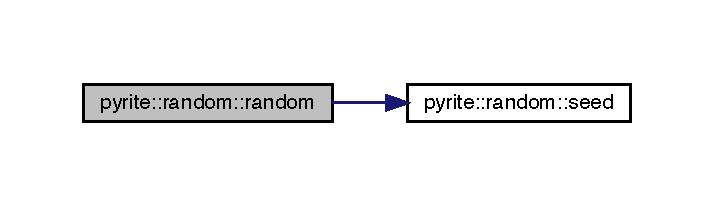
\includegraphics[width=343pt]{d2/df9/classpyrite_1_1random_a9f0f5391be20a8fdc3d6009e14dc0bfe_cgraph}
\end{center}
\end{figure}
\mbox{\Hypertarget{classpyrite_1_1random_ab3ef314958056708117ab37d2dded013}\label{classpyrite_1_1random_ab3ef314958056708117ab37d2dded013}} 
\index{pyrite\+::random@{pyrite\+::random}!random@{random}}
\index{random@{random}!pyrite\+::random@{pyrite\+::random}}
\subsubsection{\texorpdfstring{random()}{random()}\hspace{0.1cm}{\footnotesize\ttfamily [4/5]}}
{\footnotesize\ttfamily pyrite\+::random\+::random (\begin{DoxyParamCaption}\item[{\mbox{\hyperlink{classpyrite_1_1random}{random}} const \&}]{other }\end{DoxyParamCaption})}

Copy constructor.


\begin{DoxyParams}[1]{Parameters}
\mbox{\tt in}  & {\em other} & original. \\
\hline
\end{DoxyParams}
\mbox{\Hypertarget{classpyrite_1_1random_a263c5a878b5aaa150d915d765420f294}\label{classpyrite_1_1random_a263c5a878b5aaa150d915d765420f294}} 
\index{pyrite\+::random@{pyrite\+::random}!random@{random}}
\index{random@{random}!pyrite\+::random@{pyrite\+::random}}
\subsubsection{\texorpdfstring{random()}{random()}\hspace{0.1cm}{\footnotesize\ttfamily [5/5]}}
{\footnotesize\ttfamily pyrite\+::random\+::random (\begin{DoxyParamCaption}\item[{\mbox{\hyperlink{classpyrite_1_1random}{random}} \&\&}]{other }\end{DoxyParamCaption})}

Copy constructor.


\begin{DoxyParams}[1]{Parameters}
\mbox{\tt in}  & {\em other} & Move source. \\
\hline
\end{DoxyParams}
\mbox{\Hypertarget{classpyrite_1_1random_ae8d71dcc48a9eb0fe84525b368b91e05}\label{classpyrite_1_1random_ae8d71dcc48a9eb0fe84525b368b91e05}} 
\index{pyrite\+::random@{pyrite\+::random}!````~random@{$\sim$random}}
\index{````~random@{$\sim$random}!pyrite\+::random@{pyrite\+::random}}
\subsubsection{\texorpdfstring{$\sim$random()}{~random()}}
{\footnotesize\ttfamily pyrite\+::random\+::$\sim$random (\begin{DoxyParamCaption}{ }\end{DoxyParamCaption})\hspace{0.3cm}{\ttfamily [default]}}

Destructor.

Generated by compiler. 

\subsection{Member Function Documentation}
\mbox{\Hypertarget{classpyrite_1_1random_a8414030e5c428c20b8a8333542918f8c}\label{classpyrite_1_1random_a8414030e5c428c20b8a8333542918f8c}} 
\index{pyrite\+::random@{pyrite\+::random}!discard@{discard}}
\index{discard@{discard}!pyrite\+::random@{pyrite\+::random}}
\subsubsection{\texorpdfstring{discard()}{discard()}}
{\footnotesize\ttfamily void pyrite\+::random\+::discard (\begin{DoxyParamCaption}\item[{\mbox{\hyperlink{type_8hpp_a89cb75b6e56f357c2964bbd5520be899}{u64}}}]{z }\end{DoxyParamCaption})}

Advances the internal state by z times. Equivalent to calling \mbox{\hyperlink{classpyrite_1_1random_a708282ad1435ee4b9564c8e11baf43f8}{next$<$\+T$>$()}} z times and discarding the result.


\begin{DoxyParams}{Parameters}
{\em z} & Integer value specifying the number of times to advance the state by. \\
\hline
\end{DoxyParams}
\mbox{\Hypertarget{classpyrite_1_1random_a708282ad1435ee4b9564c8e11baf43f8}\label{classpyrite_1_1random_a708282ad1435ee4b9564c8e11baf43f8}} 
\index{pyrite\+::random@{pyrite\+::random}!next@{next}}
\index{next@{next}!pyrite\+::random@{pyrite\+::random}}
\subsubsection{\texorpdfstring{next()}{next()}\hspace{0.1cm}{\footnotesize\ttfamily [1/2]}}
{\footnotesize\ttfamily template$<$typename T $>$ \\
auto pyrite\+::random\+::next (\begin{DoxyParamCaption}{ }\end{DoxyParamCaption})}

Generate random number.


\begin{DoxyTemplParams}{Template Parameters}
{\em T} & Type of random number.\\
\hline
\end{DoxyTemplParams}
\begin{DoxyReturn}{Returns}
If T is integer type, return \mbox{[}std\+::numeric\+\_\+limits$<$\+T$>$\+::min(), std\+::numeric\+\_\+limits$<$\+T$>$\+::max()\mbox{]}; then if T is floating point, type return \mbox{[}0, 1\mbox{]}. 
\end{DoxyReturn}
\mbox{\Hypertarget{classpyrite_1_1random_a79e67ec7537ab7e872cb1327dbe0bb3e}\label{classpyrite_1_1random_a79e67ec7537ab7e872cb1327dbe0bb3e}} 
\index{pyrite\+::random@{pyrite\+::random}!next@{next}}
\index{next@{next}!pyrite\+::random@{pyrite\+::random}}
\subsubsection{\texorpdfstring{next()}{next()}\hspace{0.1cm}{\footnotesize\ttfamily [2/2]}}
{\footnotesize\ttfamily template$<$typename T $>$ \\
auto pyrite\+::random\+::next (\begin{DoxyParamCaption}\item[{T const \&}]{min,  }\item[{T const \&}]{max }\end{DoxyParamCaption})}

Generate random number.


\begin{DoxyTemplParams}{Template Parameters}
{\em T} & Type of random number. \\
\hline
\end{DoxyTemplParams}

\begin{DoxyParams}{Parameters}
{\em min} & Minimum value of random number \\
\hline
{\em max} & Maximum value of random number\\
\hline
\end{DoxyParams}
\begin{DoxyReturn}{Returns}
\mbox{[}min, max\mbox{]} 
\end{DoxyReturn}
\mbox{\Hypertarget{classpyrite_1_1random_aaef2fad3aa9ae947e7ed640db176373e}\label{classpyrite_1_1random_aaef2fad3aa9ae947e7ed640db176373e}} 
\index{pyrite\+::random@{pyrite\+::random}!operator"!=@{operator"!=}}
\index{operator"!=@{operator"!=}!pyrite\+::random@{pyrite\+::random}}
\subsubsection{\texorpdfstring{operator"!=()}{operator!=()}}
{\footnotesize\ttfamily bool pyrite\+::random\+::operator!= (\begin{DoxyParamCaption}\item[{\mbox{\hyperlink{classpyrite_1_1random}{random}} const \&}]{rhs }\end{DoxyParamCaption}) const\hspace{0.3cm}{\ttfamily [noexcept]}}

Compare two random object.

\begin{DoxyReturn}{Returns}
!($\ast$this != rhs); 
\end{DoxyReturn}
\mbox{\Hypertarget{classpyrite_1_1random_a3cd7cfec2938a1bd9541f34bf2b7ac77}\label{classpyrite_1_1random_a3cd7cfec2938a1bd9541f34bf2b7ac77}} 
\index{pyrite\+::random@{pyrite\+::random}!operator=@{operator=}}
\index{operator=@{operator=}!pyrite\+::random@{pyrite\+::random}}
\subsubsection{\texorpdfstring{operator=()}{operator=()}\hspace{0.1cm}{\footnotesize\ttfamily [1/2]}}
{\footnotesize\ttfamily \mbox{\hyperlink{classpyrite_1_1random}{random}} \& pyrite\+::random\+::operator= (\begin{DoxyParamCaption}\item[{\mbox{\hyperlink{classpyrite_1_1random}{random}} const \&}]{rhs }\end{DoxyParamCaption})}

Copy assignment operator. Here is the call graph for this function\+:
\nopagebreak
\begin{figure}[H]
\begin{center}
\leavevmode
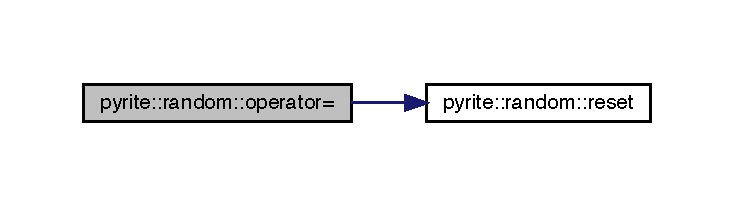
\includegraphics[width=350pt]{d2/df9/classpyrite_1_1random_a3cd7cfec2938a1bd9541f34bf2b7ac77_cgraph}
\end{center}
\end{figure}
\mbox{\Hypertarget{classpyrite_1_1random_a611890eeb411e9081e218d68bb507810}\label{classpyrite_1_1random_a611890eeb411e9081e218d68bb507810}} 
\index{pyrite\+::random@{pyrite\+::random}!operator=@{operator=}}
\index{operator=@{operator=}!pyrite\+::random@{pyrite\+::random}}
\subsubsection{\texorpdfstring{operator=()}{operator=()}\hspace{0.1cm}{\footnotesize\ttfamily [2/2]}}
{\footnotesize\ttfamily \mbox{\hyperlink{classpyrite_1_1random}{random}} \& pyrite\+::random\+::operator= (\begin{DoxyParamCaption}\item[{\mbox{\hyperlink{classpyrite_1_1random}{random}} \&\&}]{rhs }\end{DoxyParamCaption})}

Move assignment operator. \mbox{\Hypertarget{classpyrite_1_1random_a6c58ae19800d0e1f8388b6afbb79a1ba}\label{classpyrite_1_1random_a6c58ae19800d0e1f8388b6afbb79a1ba}} 
\index{pyrite\+::random@{pyrite\+::random}!operator==@{operator==}}
\index{operator==@{operator==}!pyrite\+::random@{pyrite\+::random}}
\subsubsection{\texorpdfstring{operator==()}{operator==()}}
{\footnotesize\ttfamily bool pyrite\+::random\+::operator== (\begin{DoxyParamCaption}\item[{\mbox{\hyperlink{classpyrite_1_1random}{random}} const \&}]{rhs }\end{DoxyParamCaption}) const\hspace{0.3cm}{\ttfamily [noexcept]}}

Compare two random object. Two random objects are equal when state object is the same.

\begin{DoxyReturn}{Returns}
Return true if state object is the same. 
\end{DoxyReturn}
\mbox{\Hypertarget{classpyrite_1_1random_aed264da4ddd55aab1cf72ddb091ec902}\label{classpyrite_1_1random_aed264da4ddd55aab1cf72ddb091ec902}} 
\index{pyrite\+::random@{pyrite\+::random}!reset@{reset}}
\index{reset@{reset}!pyrite\+::random@{pyrite\+::random}}
\subsubsection{\texorpdfstring{reset()}{reset()}\hspace{0.1cm}{\footnotesize\ttfamily [1/3]}}
{\footnotesize\ttfamily void pyrite\+::random\+::reset (\begin{DoxyParamCaption}{ }\end{DoxyParamCaption})}

Reset the random number generator without changing the seed. Here is the caller graph for this function\+:
\nopagebreak
\begin{figure}[H]
\begin{center}
\leavevmode
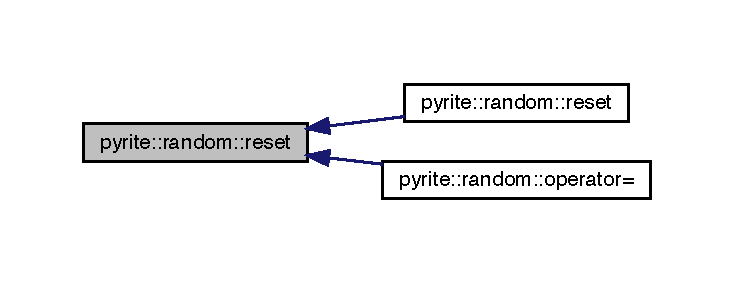
\includegraphics[width=350pt]{d2/df9/classpyrite_1_1random_aed264da4ddd55aab1cf72ddb091ec902_icgraph}
\end{center}
\end{figure}
\mbox{\Hypertarget{classpyrite_1_1random_a6d5947d6c425031e81f8488187a332f3}\label{classpyrite_1_1random_a6d5947d6c425031e81f8488187a332f3}} 
\index{pyrite\+::random@{pyrite\+::random}!reset@{reset}}
\index{reset@{reset}!pyrite\+::random@{pyrite\+::random}}
\subsubsection{\texorpdfstring{reset()}{reset()}\hspace{0.1cm}{\footnotesize\ttfamily [2/3]}}
{\footnotesize\ttfamily void pyrite\+::random\+::reset (\begin{DoxyParamCaption}\item[{\mbox{\hyperlink{classpyrite_1_1random_a936dc9fd106c9b125ccbf3aa6d525e4b}{random\+::seed\+\_\+type}}}]{seed }\end{DoxyParamCaption})}

Reset the random number generator with the new seed.


\begin{DoxyParams}{Parameters}
{\em seed} & new seed. \\
\hline
\end{DoxyParams}
Here is the call graph for this function\+:
\nopagebreak
\begin{figure}[H]
\begin{center}
\leavevmode
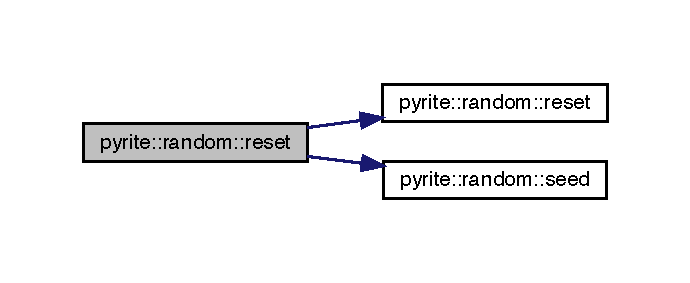
\includegraphics[width=331pt]{d2/df9/classpyrite_1_1random_a6d5947d6c425031e81f8488187a332f3_cgraph}
\end{center}
\end{figure}
\mbox{\Hypertarget{classpyrite_1_1random_a5abed1bb1fbd44ea3e62197a9b11dcd0}\label{classpyrite_1_1random_a5abed1bb1fbd44ea3e62197a9b11dcd0}} 
\index{pyrite\+::random@{pyrite\+::random}!reset@{reset}}
\index{reset@{reset}!pyrite\+::random@{pyrite\+::random}}
\subsubsection{\texorpdfstring{reset()}{reset()}\hspace{0.1cm}{\footnotesize\ttfamily [3/3]}}
{\footnotesize\ttfamily void pyrite\+::random\+::reset (\begin{DoxyParamCaption}\item[{\mbox{\hyperlink{structpyrite_1_1random__state}{random\+\_\+state}} const \&}]{state }\end{DoxyParamCaption})}

Restore ther state of random number generator from state object.


\begin{DoxyParams}{Parameters}
{\em state} & state object. \\
\hline
\end{DoxyParams}
Here is the call graph for this function\+:
\nopagebreak
\begin{figure}[H]
\begin{center}
\leavevmode
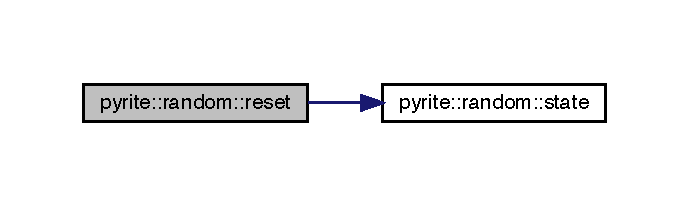
\includegraphics[width=331pt]{d2/df9/classpyrite_1_1random_a5abed1bb1fbd44ea3e62197a9b11dcd0_cgraph}
\end{center}
\end{figure}
\mbox{\Hypertarget{classpyrite_1_1random_ae3a15129c724af7168f55135226c0dfc}\label{classpyrite_1_1random_ae3a15129c724af7168f55135226c0dfc}} 
\index{pyrite\+::random@{pyrite\+::random}!seed@{seed}}
\index{seed@{seed}!pyrite\+::random@{pyrite\+::random}}
\subsubsection{\texorpdfstring{seed()}{seed()}}
{\footnotesize\ttfamily \mbox{\hyperlink{classpyrite_1_1random_a936dc9fd106c9b125ccbf3aa6d525e4b}{random\+::seed\+\_\+type}} pyrite\+::random\+::seed (\begin{DoxyParamCaption}{ }\end{DoxyParamCaption}) const\hspace{0.3cm}{\ttfamily [noexcept]}}

Get seed. Here is the caller graph for this function\+:
\nopagebreak
\begin{figure}[H]
\begin{center}
\leavevmode
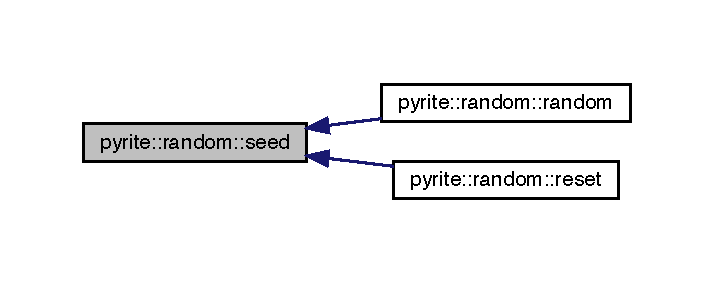
\includegraphics[width=343pt]{d2/df9/classpyrite_1_1random_ae3a15129c724af7168f55135226c0dfc_icgraph}
\end{center}
\end{figure}
\mbox{\Hypertarget{classpyrite_1_1random_a25c469022ddee73c6a4ecce2814d22d4}\label{classpyrite_1_1random_a25c469022ddee73c6a4ecce2814d22d4}} 
\index{pyrite\+::random@{pyrite\+::random}!state@{state}}
\index{state@{state}!pyrite\+::random@{pyrite\+::random}}
\subsubsection{\texorpdfstring{state()}{state()}}
{\footnotesize\ttfamily \mbox{\hyperlink{structpyrite_1_1random__state}{random\+\_\+state}} pyrite\+::random\+::state (\begin{DoxyParamCaption}{ }\end{DoxyParamCaption}) const\hspace{0.3cm}{\ttfamily [noexcept]}}

Get object state. Here is the caller graph for this function\+:
\nopagebreak
\begin{figure}[H]
\begin{center}
\leavevmode
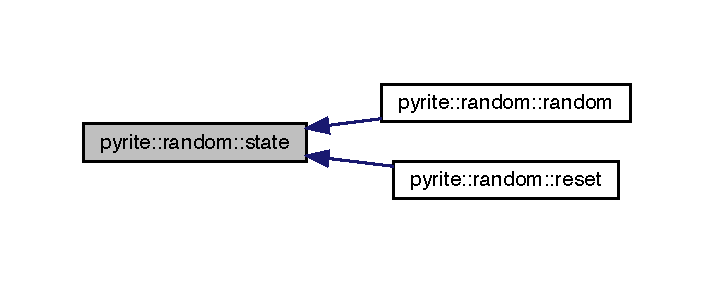
\includegraphics[width=343pt]{d2/df9/classpyrite_1_1random_a25c469022ddee73c6a4ecce2814d22d4_icgraph}
\end{center}
\end{figure}


The documentation for this class was generated from the following files\+:\begin{DoxyCompactItemize}
\item 
/\+Users/masato.\+tanaka/\+Development/cpp/pyrite/pyrite/random/\mbox{\hyperlink{random_2random_8hpp}{random.\+hpp}}\item 
/\+Users/masato.\+tanaka/\+Development/cpp/pyrite/pyrite/random/\mbox{\hyperlink{random_8inl}{random.\+inl}}\end{DoxyCompactItemize}

\hypertarget{structpyrite_1_1random__state}{}\section{pyrite\+:\+:random\+\_\+state Struct Reference}
\label{structpyrite_1_1random__state}\index{pyrite\+::random\+\_\+state@{pyrite\+::random\+\_\+state}}


{\ttfamily \#include $<$random\+\_\+state.\+hpp$>$}

\subsection*{Public Attributes}
\begin{DoxyCompactItemize}
\item 
\mbox{\Hypertarget{structpyrite_1_1random__state_a0e2c55b67459b8e81c7d94cde7aab26a}\label{structpyrite_1_1random__state_a0e2c55b67459b8e81c7d94cde7aab26a}} 
\mbox{\hyperlink{type_8hpp_a89cb75b6e56f357c2964bbd5520be899}{u64}} \mbox{\hyperlink{structpyrite_1_1random__state_a0e2c55b67459b8e81c7d94cde7aab26a}{seed}} \{0u\}
\begin{DoxyCompactList}\small\item\em seed \end{DoxyCompactList}\item 
\mbox{\Hypertarget{structpyrite_1_1random__state_ad78110ffa166ae4f6506f81c7084e42a}\label{structpyrite_1_1random__state_ad78110ffa166ae4f6506f81c7084e42a}} 
\mbox{\hyperlink{type_8hpp_a89cb75b6e56f357c2964bbd5520be899}{u64}} \mbox{\hyperlink{structpyrite_1_1random__state_ad78110ffa166ae4f6506f81c7084e42a}{count}} \{0u\}
\begin{DoxyCompactList}\small\item\em count of generated random number. \end{DoxyCompactList}\end{DoxyCompactItemize}


\subsection{Detailed Description}
State of \mbox{\hyperlink{classpyrite_1_1random}{pyrite\+::random}} 

The documentation for this struct was generated from the following file\+:\begin{DoxyCompactItemize}
\item 
/\+Users/masato.\+tanaka/\+Development/cpp/pyrite/pyrite/random/\mbox{\hyperlink{random__state_8hpp}{random\+\_\+state.\+hpp}}\end{DoxyCompactItemize}

\hypertarget{structpyrite_1_1mpl_1_1replace__if}{}\section{pyrite\+:\+:mpl\+:\+:replace\+\_\+if$<$ List, Pred, New\+Type $>$ Struct Template Reference}
\label{structpyrite_1_1mpl_1_1replace__if}\index{pyrite\+::mpl\+::replace\+\_\+if$<$ List, Pred, New\+Type $>$@{pyrite\+::mpl\+::replace\+\_\+if$<$ List, Pred, New\+Type $>$}}
\subsection*{Public Types}
\begin{DoxyCompactItemize}
\item 
\mbox{\Hypertarget{structpyrite_1_1mpl_1_1replace__if_a5bc0ece826e82bfa5861bb96f939f242}\label{structpyrite_1_1mpl_1_1replace__if_a5bc0ece826e82bfa5861bb96f939f242}} 
using {\bfseries type} = transform\+\_\+t$<$ List, replace\+\_\+pred $>$
\end{DoxyCompactItemize}


The documentation for this struct was generated from the following file\+:\begin{DoxyCompactItemize}
\item 
/\+Users/masato.\+tanaka/\+Development/cpp/pyrite/pyrite/mpl/type\+\_\+list/\mbox{\hyperlink{replace__if_8hpp}{replace\+\_\+if.\+hpp}}\end{DoxyCompactItemize}

\hypertarget{structpyrite_1_1mpl_1_1reverse}{}\section{pyrite\+:\+:mpl\+:\+:reverse$<$ List $>$ Struct Template Reference}
\label{structpyrite_1_1mpl_1_1reverse}\index{pyrite\+::mpl\+::reverse$<$ List $>$@{pyrite\+::mpl\+::reverse$<$ List $>$}}
\subsection*{Public Types}
\begin{DoxyCompactItemize}
\item 
\mbox{\Hypertarget{structpyrite_1_1mpl_1_1reverse_ad0fc79c5adba1db095b4dd23d979e24f}\label{structpyrite_1_1mpl_1_1reverse_ad0fc79c5adba1db095b4dd23d979e24f}} 
using {\bfseries type} = reverse\+\_\+\+::sequence\+\_\+to\+\_\+list$<$ List, reversed\+\_\+sequence $>$
\end{DoxyCompactItemize}


The documentation for this struct was generated from the following file\+:\begin{DoxyCompactItemize}
\item 
/\+Users/masato.\+tanaka/\+Development/cpp/pyrite/pyrite/mpl/type\+\_\+list/\mbox{\hyperlink{reverse_8hpp}{reverse.\+hpp}}\end{DoxyCompactItemize}

\hypertarget{structpyrite_1_1mpl_1_1reverse_3_01type__list_3_4_01_4}{}\section{pyrite\+:\+:mpl\+:\+:reverse$<$ type\+\_\+list$<$$>$ $>$ Struct Template Reference}
\label{structpyrite_1_1mpl_1_1reverse_3_01type__list_3_4_01_4}\index{pyrite\+::mpl\+::reverse$<$ type\+\_\+list$<$$>$ $>$@{pyrite\+::mpl\+::reverse$<$ type\+\_\+list$<$$>$ $>$}}
\subsection*{Public Types}
\begin{DoxyCompactItemize}
\item 
\mbox{\Hypertarget{structpyrite_1_1mpl_1_1reverse_3_01type__list_3_4_01_4_a32ca95170698543f6fb0b12642397f80}\label{structpyrite_1_1mpl_1_1reverse_3_01type__list_3_4_01_4_a32ca95170698543f6fb0b12642397f80}} 
using {\bfseries type} = \mbox{\hyperlink{structpyrite_1_1core_1_1mpl_1_1type__list}{type\+\_\+list}}$<$$>$
\end{DoxyCompactItemize}


The documentation for this struct was generated from the following file\+:\begin{DoxyCompactItemize}
\item 
/\+Users/masato.\+tanaka/\+Development/cpp/pyrite/pyrite/mpl/type\+\_\+list/\mbox{\hyperlink{reverse_8hpp}{reverse.\+hpp}}\end{DoxyCompactItemize}

\hypertarget{classpyrite_1_1scope__exit}{}\section{pyrite\+:\+:scope\+\_\+exit$<$ F $>$ Class Template Reference}
\label{classpyrite_1_1scope__exit}\index{pyrite\+::scope\+\_\+exit$<$ F $>$@{pyrite\+::scope\+\_\+exit$<$ F $>$}}


{\ttfamily \#include $<$scope\+\_\+exit.\+hpp$>$}



Inheritance diagram for pyrite\+:\+:scope\+\_\+exit$<$ F $>$\+:
\nopagebreak
\begin{figure}[H]
\begin{center}
\leavevmode
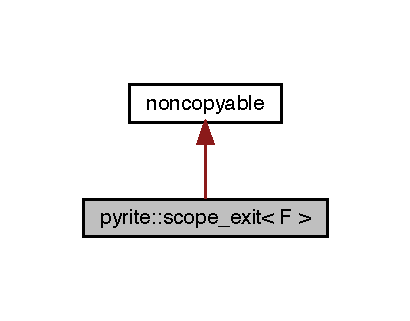
\includegraphics[width=197pt]{dc/d46/classpyrite_1_1scope__exit__inherit__graph}
\end{center}
\end{figure}


Collaboration diagram for pyrite\+:\+:scope\+\_\+exit$<$ F $>$\+:
\nopagebreak
\begin{figure}[H]
\begin{center}
\leavevmode
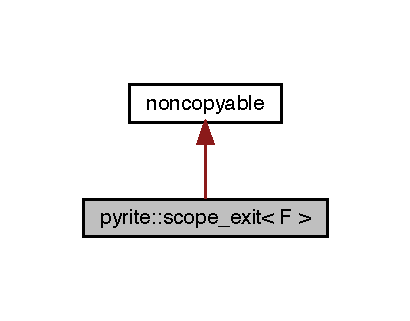
\includegraphics[width=197pt]{d3/df8/classpyrite_1_1scope__exit__coll__graph}
\end{center}
\end{figure}
\subsection*{Public Member Functions}
\begin{DoxyCompactItemize}
\item 
\mbox{\hyperlink{classpyrite_1_1scope__exit_aa91a09b5b29bd1f7596eb35348b55b34}{scope\+\_\+exit}} (F const \&function)
\item 
\mbox{\hyperlink{classpyrite_1_1scope__exit_a35cb6b81607b2ea3ca006a387c3d669f}{scope\+\_\+exit}} (\mbox{\hyperlink{classpyrite_1_1scope__exit}{scope\+\_\+exit}} \&\&)=default
\item 
\mbox{\hyperlink{classpyrite_1_1scope__exit_a724fd7a0fc8fe24fe7ee50f3be68be1f}{$\sim$scope\+\_\+exit}} ()
\item 
\mbox{\hyperlink{classpyrite_1_1scope__exit}{scope\+\_\+exit}} \& \mbox{\hyperlink{classpyrite_1_1scope__exit_a1b2d819eb3eba7a77102a1df5f5a2668}{operator=}} (\mbox{\hyperlink{classpyrite_1_1scope__exit}{scope\+\_\+exit}} \&\&)=default
\end{DoxyCompactItemize}


\subsection{Detailed Description}
\subsubsection*{template$<$typename F$>$\newline
class pyrite\+::scope\+\_\+exit$<$ F $>$}

Call the function when you exit the scope. 
\begin{DoxyTemplParams}{Template Parameters}
{\em F} & The type of function to call. \\
\hline
\end{DoxyTemplParams}


\subsection{Constructor \& Destructor Documentation}
\mbox{\Hypertarget{classpyrite_1_1scope__exit_aa91a09b5b29bd1f7596eb35348b55b34}\label{classpyrite_1_1scope__exit_aa91a09b5b29bd1f7596eb35348b55b34}} 
\index{pyrite\+::scope\+\_\+exit@{pyrite\+::scope\+\_\+exit}!scope\+\_\+exit@{scope\+\_\+exit}}
\index{scope\+\_\+exit@{scope\+\_\+exit}!pyrite\+::scope\+\_\+exit@{pyrite\+::scope\+\_\+exit}}
\subsubsection{\texorpdfstring{scope\+\_\+exit()}{scope\_exit()}\hspace{0.1cm}{\footnotesize\ttfamily [1/2]}}
{\footnotesize\ttfamily template$<$typename F $>$ \\
\mbox{\hyperlink{classpyrite_1_1scope__exit}{pyrite\+::scope\+\_\+exit}}$<$ F $>$\+::\mbox{\hyperlink{classpyrite_1_1scope__exit}{scope\+\_\+exit}} (\begin{DoxyParamCaption}\item[{F const \&}]{function }\end{DoxyParamCaption})\hspace{0.3cm}{\ttfamily [inline]}}

Constructor.


\begin{DoxyParams}[1]{Parameters}
\mbox{\tt in}  & {\em function} & Function to be called when exiting the scope. \\
\hline
\end{DoxyParams}
\mbox{\Hypertarget{classpyrite_1_1scope__exit_a35cb6b81607b2ea3ca006a387c3d669f}\label{classpyrite_1_1scope__exit_a35cb6b81607b2ea3ca006a387c3d669f}} 
\index{pyrite\+::scope\+\_\+exit@{pyrite\+::scope\+\_\+exit}!scope\+\_\+exit@{scope\+\_\+exit}}
\index{scope\+\_\+exit@{scope\+\_\+exit}!pyrite\+::scope\+\_\+exit@{pyrite\+::scope\+\_\+exit}}
\subsubsection{\texorpdfstring{scope\+\_\+exit()}{scope\_exit()}\hspace{0.1cm}{\footnotesize\ttfamily [2/2]}}
{\footnotesize\ttfamily template$<$typename F $>$ \\
\mbox{\hyperlink{classpyrite_1_1scope__exit}{pyrite\+::scope\+\_\+exit}}$<$ F $>$\+::\mbox{\hyperlink{classpyrite_1_1scope__exit}{scope\+\_\+exit}} (\begin{DoxyParamCaption}\item[{\mbox{\hyperlink{classpyrite_1_1scope__exit}{scope\+\_\+exit}}$<$ F $>$ \&\&}]{ }\end{DoxyParamCaption})\hspace{0.3cm}{\ttfamily [default]}}

Move constructor. \mbox{\Hypertarget{classpyrite_1_1scope__exit_a724fd7a0fc8fe24fe7ee50f3be68be1f}\label{classpyrite_1_1scope__exit_a724fd7a0fc8fe24fe7ee50f3be68be1f}} 
\index{pyrite\+::scope\+\_\+exit@{pyrite\+::scope\+\_\+exit}!````~scope\+\_\+exit@{$\sim$scope\+\_\+exit}}
\index{````~scope\+\_\+exit@{$\sim$scope\+\_\+exit}!pyrite\+::scope\+\_\+exit@{pyrite\+::scope\+\_\+exit}}
\subsubsection{\texorpdfstring{$\sim$scope\+\_\+exit()}{~scope\_exit()}}
{\footnotesize\ttfamily template$<$typename F $>$ \\
\mbox{\hyperlink{classpyrite_1_1scope__exit}{pyrite\+::scope\+\_\+exit}}$<$ F $>$\+::$\sim$\mbox{\hyperlink{classpyrite_1_1scope__exit}{scope\+\_\+exit}} (\begin{DoxyParamCaption}{ }\end{DoxyParamCaption})\hspace{0.3cm}{\ttfamily [inline]}}

Destructor. Call the function received in the constructor. 

\subsection{Member Function Documentation}
\mbox{\Hypertarget{classpyrite_1_1scope__exit_a1b2d819eb3eba7a77102a1df5f5a2668}\label{classpyrite_1_1scope__exit_a1b2d819eb3eba7a77102a1df5f5a2668}} 
\index{pyrite\+::scope\+\_\+exit@{pyrite\+::scope\+\_\+exit}!operator=@{operator=}}
\index{operator=@{operator=}!pyrite\+::scope\+\_\+exit@{pyrite\+::scope\+\_\+exit}}
\subsubsection{\texorpdfstring{operator=()}{operator=()}}
{\footnotesize\ttfamily template$<$typename F $>$ \\
\mbox{\hyperlink{classpyrite_1_1scope__exit}{scope\+\_\+exit}}\& \mbox{\hyperlink{classpyrite_1_1scope__exit}{pyrite\+::scope\+\_\+exit}}$<$ F $>$\+::operator= (\begin{DoxyParamCaption}\item[{\mbox{\hyperlink{classpyrite_1_1scope__exit}{scope\+\_\+exit}}$<$ F $>$ \&\&}]{ }\end{DoxyParamCaption})\hspace{0.3cm}{\ttfamily [default]}}

Move assignment operator. 

The documentation for this class was generated from the following file\+:\begin{DoxyCompactItemize}
\item 
/\+Users/masato.\+tanaka/\+Development/cpp/pyrite/pyrite/\mbox{\hyperlink{scope__exit_8hpp}{scope\+\_\+exit.\+hpp}}\end{DoxyCompactItemize}

\hypertarget{structpyrite_1_1mpl_1_1reverse___1_1sequence__reverse}{}\section{pyrite\+:\+:mpl\+:\+:reverse\+\_\+\+:\+:sequence\+\_\+reverse$<$ Sequence $>$ Struct Template Reference}
\label{structpyrite_1_1mpl_1_1reverse___1_1sequence__reverse}\index{pyrite\+::mpl\+::reverse\+\_\+\+::sequence\+\_\+reverse$<$ Sequence $>$@{pyrite\+::mpl\+::reverse\+\_\+\+::sequence\+\_\+reverse$<$ Sequence $>$}}


The documentation for this struct was generated from the following file\+:\begin{DoxyCompactItemize}
\item 
/\+Users/masato.\+tanaka/\+Development/cpp/pyrite/pyrite/mpl/type\+\_\+list/\mbox{\hyperlink{reverse_8hpp}{reverse.\+hpp}}\end{DoxyCompactItemize}

\hypertarget{structpyrite_1_1mpl_1_1reverse___1_1sequence__reverse_3_01std_1_1index__sequence_3_01_index_8_8_8_01_4_01_4}{}\section{pyrite\+:\+:mpl\+:\+:reverse\+\_\+\+:\+:sequence\+\_\+reverse$<$ std\+:\+:index\+\_\+sequence$<$ Index... $>$ $>$ Struct Template Reference}
\label{structpyrite_1_1mpl_1_1reverse___1_1sequence__reverse_3_01std_1_1index__sequence_3_01_index_8_8_8_01_4_01_4}\index{pyrite\+::mpl\+::reverse\+\_\+\+::sequence\+\_\+reverse$<$ std\+::index\+\_\+sequence$<$ Index... $>$ $>$@{pyrite\+::mpl\+::reverse\+\_\+\+::sequence\+\_\+reverse$<$ std\+::index\+\_\+sequence$<$ Index... $>$ $>$}}
\subsection*{Public Types}
\begin{DoxyCompactItemize}
\item 
\mbox{\Hypertarget{structpyrite_1_1mpl_1_1reverse___1_1sequence__reverse_3_01std_1_1index__sequence_3_01_index_8_8_8_01_4_01_4_a6893882c77aad4f277cdc2f453811f50}\label{structpyrite_1_1mpl_1_1reverse___1_1sequence__reverse_3_01std_1_1index__sequence_3_01_index_8_8_8_01_4_01_4_a6893882c77aad4f277cdc2f453811f50}} 
using {\bfseries type} = std\+::index\+\_\+sequence$<$(sizeof...(Index) -\/ 1 -\/ Index)... $>$
\end{DoxyCompactItemize}


The documentation for this struct was generated from the following file\+:\begin{DoxyCompactItemize}
\item 
/\+Users/masato.\+tanaka/\+Development/cpp/pyrite/pyrite/mpl/type\+\_\+list/\mbox{\hyperlink{reverse_8hpp}{reverse.\+hpp}}\end{DoxyCompactItemize}

\hypertarget{structpyrite_1_1mpl_1_1at___1_1sequence__to__list}{}\section{pyrite\+:\+:mpl\+:\+:at\+\_\+\+:\+:sequence\+\_\+to\+\_\+list$<$ Sequence $>$ Struct Template Reference}
\label{structpyrite_1_1mpl_1_1at___1_1sequence__to__list}\index{pyrite\+::mpl\+::at\+\_\+\+::sequence\+\_\+to\+\_\+list$<$ Sequence $>$@{pyrite\+::mpl\+::at\+\_\+\+::sequence\+\_\+to\+\_\+list$<$ Sequence $>$}}


The documentation for this struct was generated from the following file\+:\begin{DoxyCompactItemize}
\item 
/\+Users/masato.\+tanaka/\+Development/cpp/pyrite/pyrite/mpl/type\+\_\+list/\mbox{\hyperlink{at_8hpp}{at.\+hpp}}\end{DoxyCompactItemize}

\hypertarget{structpyrite_1_1mpl_1_1make__type__list___1_1sequence__to__list}{}\section{pyrite\+:\+:mpl\+:\+:make\+\_\+type\+\_\+list\+\_\+\+:\+:sequence\+\_\+to\+\_\+list$<$ T, Sequence $>$ Struct Template Reference}
\label{structpyrite_1_1mpl_1_1make__type__list___1_1sequence__to__list}\index{pyrite\+::mpl\+::make\+\_\+type\+\_\+list\+\_\+\+::sequence\+\_\+to\+\_\+list$<$ T, Sequence $>$@{pyrite\+::mpl\+::make\+\_\+type\+\_\+list\+\_\+\+::sequence\+\_\+to\+\_\+list$<$ T, Sequence $>$}}


The documentation for this struct was generated from the following file\+:\begin{DoxyCompactItemize}
\item 
/\+Users/masato.\+tanaka/\+Development/cpp/pyrite/pyrite/mpl/type\+\_\+list/\mbox{\hyperlink{make__type__list_8hpp}{make\+\_\+type\+\_\+list.\+hpp}}\end{DoxyCompactItemize}

\hypertarget{structpyrite_1_1mpl_1_1at___1_1sequence__to__list_3_01std_1_1index__sequence_3_01_index_8_8_8_01_4_01_4}{}\section{pyrite\+:\+:mpl\+:\+:at\+\_\+\+:\+:sequence\+\_\+to\+\_\+list$<$ std\+:\+:index\+\_\+sequence$<$ Index... $>$ $>$ Struct Template Reference}
\label{structpyrite_1_1mpl_1_1at___1_1sequence__to__list_3_01std_1_1index__sequence_3_01_index_8_8_8_01_4_01_4}\index{pyrite\+::mpl\+::at\+\_\+\+::sequence\+\_\+to\+\_\+list$<$ std\+::index\+\_\+sequence$<$ Index... $>$ $>$@{pyrite\+::mpl\+::at\+\_\+\+::sequence\+\_\+to\+\_\+list$<$ std\+::index\+\_\+sequence$<$ Index... $>$ $>$}}
\subsection*{Public Types}
\begin{DoxyCompactItemize}
\item 
\mbox{\Hypertarget{structpyrite_1_1mpl_1_1at___1_1sequence__to__list_3_01std_1_1index__sequence_3_01_index_8_8_8_01_4_01_4_a9560b86188e9174b37f30bee12db4576}\label{structpyrite_1_1mpl_1_1at___1_1sequence__to__list_3_01std_1_1index__sequence_3_01_index_8_8_8_01_4_01_4_a9560b86188e9174b37f30bee12db4576}} 
using {\bfseries type} = \mbox{\hyperlink{structpyrite_1_1core_1_1mpl_1_1type__list}{type\+\_\+list}}$<$ std\+::integral\+\_\+constant$<$ std\+::size\+\_\+t, Index $>$... $>$
\end{DoxyCompactItemize}


The documentation for this struct was generated from the following file\+:\begin{DoxyCompactItemize}
\item 
/\+Users/masato.\+tanaka/\+Development/cpp/pyrite/pyrite/mpl/type\+\_\+list/\mbox{\hyperlink{at_8hpp}{at.\+hpp}}\end{DoxyCompactItemize}

\hypertarget{structpyrite_1_1mpl_1_1make__type__list___1_1sequence__to__list_3_01_t_00_01std_1_1index__sequence_3_01_index_8_8_8_01_4_01_4}{}\section{pyrite\+:\+:mpl\+:\+:make\+\_\+type\+\_\+list\+\_\+\+:\+:sequence\+\_\+to\+\_\+list$<$ T, std\+:\+:index\+\_\+sequence$<$ Index... $>$ $>$ Struct Template Reference}
\label{structpyrite_1_1mpl_1_1make__type__list___1_1sequence__to__list_3_01_t_00_01std_1_1index__sequence_3_01_index_8_8_8_01_4_01_4}\index{pyrite\+::mpl\+::make\+\_\+type\+\_\+list\+\_\+\+::sequence\+\_\+to\+\_\+list$<$ T, std\+::index\+\_\+sequence$<$ Index... $>$ $>$@{pyrite\+::mpl\+::make\+\_\+type\+\_\+list\+\_\+\+::sequence\+\_\+to\+\_\+list$<$ T, std\+::index\+\_\+sequence$<$ Index... $>$ $>$}}
\subsection*{Public Types}
\begin{DoxyCompactItemize}
\item 
\mbox{\Hypertarget{structpyrite_1_1mpl_1_1make__type__list___1_1sequence__to__list_3_01_t_00_01std_1_1index__sequence_3_01_index_8_8_8_01_4_01_4_a0a6a63ede5bdaed5db16c9dc034e4b7f}\label{structpyrite_1_1mpl_1_1make__type__list___1_1sequence__to__list_3_01_t_00_01std_1_1index__sequence_3_01_index_8_8_8_01_4_01_4_a0a6a63ede5bdaed5db16c9dc034e4b7f}} 
using {\bfseries type} = decltype(apply())
\end{DoxyCompactItemize}


The documentation for this struct was generated from the following file\+:\begin{DoxyCompactItemize}
\item 
/\+Users/masato.\+tanaka/\+Development/cpp/pyrite/pyrite/mpl/type\+\_\+list/\mbox{\hyperlink{make__type__list_8hpp}{make\+\_\+type\+\_\+list.\+hpp}}\end{DoxyCompactItemize}

\hypertarget{structpyrite_1_1mpl_1_1reverse___1_1sequence__to__list__}{}\section{pyrite\+:\+:mpl\+:\+:reverse\+\_\+\+:\+:sequence\+\_\+to\+\_\+list\+\_\+$<$ List, Sequence $>$ Struct Template Reference}
\label{structpyrite_1_1mpl_1_1reverse___1_1sequence__to__list__}\index{pyrite\+::mpl\+::reverse\+\_\+\+::sequence\+\_\+to\+\_\+list\+\_\+$<$ List, Sequence $>$@{pyrite\+::mpl\+::reverse\+\_\+\+::sequence\+\_\+to\+\_\+list\+\_\+$<$ List, Sequence $>$}}


The documentation for this struct was generated from the following file\+:\begin{DoxyCompactItemize}
\item 
/\+Users/masato.\+tanaka/\+Development/cpp/pyrite/pyrite/mpl/type\+\_\+list/\mbox{\hyperlink{reverse_8hpp}{reverse.\+hpp}}\end{DoxyCompactItemize}

\hypertarget{structpyrite_1_1mpl_1_1reverse___1_1sequence__to__list___3_01_list_00_01std_1_1index__sequence_3_01_index_8_8_8_01_4_01_4}{}\section{pyrite\+:\+:mpl\+:\+:reverse\+\_\+\+:\+:sequence\+\_\+to\+\_\+list\+\_\+$<$ List, std\+:\+:index\+\_\+sequence$<$ Index... $>$ $>$ Struct Template Reference}
\label{structpyrite_1_1mpl_1_1reverse___1_1sequence__to__list___3_01_list_00_01std_1_1index__sequence_3_01_index_8_8_8_01_4_01_4}\index{pyrite\+::mpl\+::reverse\+\_\+\+::sequence\+\_\+to\+\_\+list\+\_\+$<$ List, std\+::index\+\_\+sequence$<$ Index... $>$ $>$@{pyrite\+::mpl\+::reverse\+\_\+\+::sequence\+\_\+to\+\_\+list\+\_\+$<$ List, std\+::index\+\_\+sequence$<$ Index... $>$ $>$}}
\subsection*{Public Types}
\begin{DoxyCompactItemize}
\item 
\mbox{\Hypertarget{structpyrite_1_1mpl_1_1reverse___1_1sequence__to__list___3_01_list_00_01std_1_1index__sequence_3_01_index_8_8_8_01_4_01_4_a1340c46dbbd09b4ac3e958df00bf7bf6}\label{structpyrite_1_1mpl_1_1reverse___1_1sequence__to__list___3_01_list_00_01std_1_1index__sequence_3_01_index_8_8_8_01_4_01_4_a1340c46dbbd09b4ac3e958df00bf7bf6}} 
using {\bfseries type} = \mbox{\hyperlink{structpyrite_1_1core_1_1mpl_1_1type__list}{type\+\_\+list}}$<$ at\+\_\+t$<$ List, Index $>$... $>$
\end{DoxyCompactItemize}


The documentation for this struct was generated from the following file\+:\begin{DoxyCompactItemize}
\item 
/\+Users/masato.\+tanaka/\+Development/cpp/pyrite/pyrite/mpl/type\+\_\+list/\mbox{\hyperlink{reverse_8hpp}{reverse.\+hpp}}\end{DoxyCompactItemize}

\hypertarget{classpyrite_1_1singleton}{}\section{pyrite\+:\+:singleton$<$ T $>$ Class Template Reference}
\label{classpyrite_1_1singleton}\index{pyrite\+::singleton$<$ T $>$@{pyrite\+::singleton$<$ T $>$}}


{\ttfamily \#include $<$singleton.\+hpp$>$}



Inheritance diagram for pyrite\+:\+:singleton$<$ T $>$\+:
\nopagebreak
\begin{figure}[H]
\begin{center}
\leavevmode
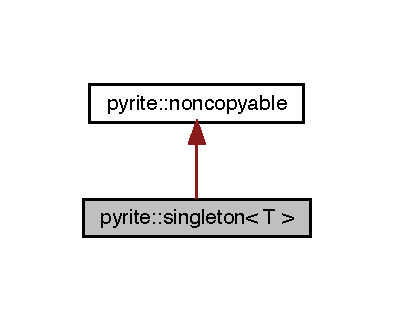
\includegraphics[width=189pt]{dc/d66/classpyrite_1_1singleton__inherit__graph}
\end{center}
\end{figure}


Collaboration diagram for pyrite\+:\+:singleton$<$ T $>$\+:
\nopagebreak
\begin{figure}[H]
\begin{center}
\leavevmode
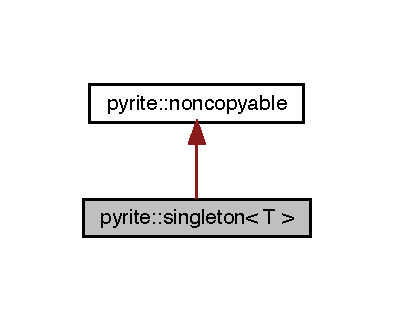
\includegraphics[width=189pt]{d3/dd3/classpyrite_1_1singleton__coll__graph}
\end{center}
\end{figure}
\subsection*{Static Public Member Functions}
\begin{DoxyCompactItemize}
\item 
static std\+::shared\+\_\+ptr$<$ T $>$ \mbox{\hyperlink{classpyrite_1_1singleton_a60ded278bfa70dcd8d0099ce3016ca40}{instance}} ()
\end{DoxyCompactItemize}
\subsection*{Protected Member Functions}
\begin{DoxyCompactItemize}
\item 
\mbox{\hyperlink{classpyrite_1_1singleton_afda9f6dd559bbb33d00d2a9ed4957e08}{singleton}} ()=default
\item 
virtual \mbox{\hyperlink{classpyrite_1_1singleton_a7255eef299d5121b3a57d4c808776847}{$\sim$singleton}} ()=default
\end{DoxyCompactItemize}


\subsection{Detailed Description}
\subsubsection*{template$<$typename T$>$\newline
class pyrite\+::singleton$<$ T $>$}

Classes that inherit the singleton class are guaranteed to have only one instance. 
\begin{DoxyParams}{Parameters}
{\em T} & Type to make singleton. \\
\hline
\end{DoxyParams}


\subsection{Constructor \& Destructor Documentation}
\mbox{\Hypertarget{classpyrite_1_1singleton_afda9f6dd559bbb33d00d2a9ed4957e08}\label{classpyrite_1_1singleton_afda9f6dd559bbb33d00d2a9ed4957e08}} 
\index{pyrite\+::singleton@{pyrite\+::singleton}!singleton@{singleton}}
\index{singleton@{singleton}!pyrite\+::singleton@{pyrite\+::singleton}}
\subsubsection{\texorpdfstring{singleton()}{singleton()}}
{\footnotesize\ttfamily template$<$typename T $>$ \\
\mbox{\hyperlink{classpyrite_1_1singleton}{pyrite\+::singleton}}$<$ T $>$\+::\mbox{\hyperlink{classpyrite_1_1singleton}{singleton}} (\begin{DoxyParamCaption}{ }\end{DoxyParamCaption})\hspace{0.3cm}{\ttfamily [protected]}, {\ttfamily [default]}}

Default constructor. \mbox{\Hypertarget{classpyrite_1_1singleton_a7255eef299d5121b3a57d4c808776847}\label{classpyrite_1_1singleton_a7255eef299d5121b3a57d4c808776847}} 
\index{pyrite\+::singleton@{pyrite\+::singleton}!````~singleton@{$\sim$singleton}}
\index{````~singleton@{$\sim$singleton}!pyrite\+::singleton@{pyrite\+::singleton}}
\subsubsection{\texorpdfstring{$\sim$singleton()}{~singleton()}}
{\footnotesize\ttfamily template$<$typename T $>$ \\
virtual \mbox{\hyperlink{classpyrite_1_1singleton}{pyrite\+::singleton}}$<$ T $>$\+::$\sim$\mbox{\hyperlink{classpyrite_1_1singleton}{singleton}} (\begin{DoxyParamCaption}{ }\end{DoxyParamCaption})\hspace{0.3cm}{\ttfamily [protected]}, {\ttfamily [virtual]}, {\ttfamily [default]}}

Virtual destructor. 

\subsection{Member Function Documentation}
\mbox{\Hypertarget{classpyrite_1_1singleton_a60ded278bfa70dcd8d0099ce3016ca40}\label{classpyrite_1_1singleton_a60ded278bfa70dcd8d0099ce3016ca40}} 
\index{pyrite\+::singleton@{pyrite\+::singleton}!instance@{instance}}
\index{instance@{instance}!pyrite\+::singleton@{pyrite\+::singleton}}
\subsubsection{\texorpdfstring{instance()}{instance()}}
{\footnotesize\ttfamily template$<$typename T $>$ \\
static std\+::shared\+\_\+ptr$<$T$>$ \mbox{\hyperlink{classpyrite_1_1singleton}{pyrite\+::singleton}}$<$ T $>$\+::instance (\begin{DoxyParamCaption}{ }\end{DoxyParamCaption})\hspace{0.3cm}{\ttfamily [inline]}, {\ttfamily [static]}}

Get an instance. If the instance does not exist, it is created. \begin{DoxyReturn}{Returns}
instance 
\end{DoxyReturn}


The documentation for this class was generated from the following file\+:\begin{DoxyCompactItemize}
\item 
/\+Users/masato.\+tanaka/\+Development/cpp/pyrite/pyrite/\mbox{\hyperlink{singleton_8hpp}{singleton.\+hpp}}\end{DoxyCompactItemize}

\hypertarget{classpyrite_1_1singleton__traits}{}\section{pyrite\+:\+:singleton\+\_\+traits$<$ T $>$ Class Template Reference}
\label{classpyrite_1_1singleton__traits}\index{pyrite\+::singleton\+\_\+traits$<$ T $>$@{pyrite\+::singleton\+\_\+traits$<$ T $>$}}
\subsection*{Static Public Member Functions}
\begin{DoxyCompactItemize}
\item 
static T $\ast$ \mbox{\hyperlink{classpyrite_1_1singleton__traits_a330f3723ce3b87978b6d45955be7950f}{create}} ()
\item 
static void \mbox{\hyperlink{classpyrite_1_1singleton__traits_a5ab8adb032a935f6e3a164bac97d2c93}{destroy}} (T $\ast$\&ptr)
\end{DoxyCompactItemize}


\subsection{Member Function Documentation}
\mbox{\Hypertarget{classpyrite_1_1singleton__traits_a330f3723ce3b87978b6d45955be7950f}\label{classpyrite_1_1singleton__traits_a330f3723ce3b87978b6d45955be7950f}} 
\index{pyrite\+::singleton\+\_\+traits@{pyrite\+::singleton\+\_\+traits}!create@{create}}
\index{create@{create}!pyrite\+::singleton\+\_\+traits@{pyrite\+::singleton\+\_\+traits}}
\subsubsection{\texorpdfstring{create()}{create()}}
{\footnotesize\ttfamily template$<$typename T $>$ \\
static T$\ast$ \mbox{\hyperlink{classpyrite_1_1singleton__traits}{pyrite\+::singleton\+\_\+traits}}$<$ T $>$\+::create (\begin{DoxyParamCaption}{ }\end{DoxyParamCaption})\hspace{0.3cm}{\ttfamily [inline]}, {\ttfamily [static]}}

Create an instance. \begin{DoxyReturn}{Returns}
A pointer to the created instance. 
\end{DoxyReturn}
\mbox{\Hypertarget{classpyrite_1_1singleton__traits_a5ab8adb032a935f6e3a164bac97d2c93}\label{classpyrite_1_1singleton__traits_a5ab8adb032a935f6e3a164bac97d2c93}} 
\index{pyrite\+::singleton\+\_\+traits@{pyrite\+::singleton\+\_\+traits}!destroy@{destroy}}
\index{destroy@{destroy}!pyrite\+::singleton\+\_\+traits@{pyrite\+::singleton\+\_\+traits}}
\subsubsection{\texorpdfstring{destroy()}{destroy()}}
{\footnotesize\ttfamily template$<$typename T $>$ \\
static void \mbox{\hyperlink{classpyrite_1_1singleton__traits}{pyrite\+::singleton\+\_\+traits}}$<$ T $>$\+::destroy (\begin{DoxyParamCaption}\item[{T $\ast$\&}]{ptr }\end{DoxyParamCaption})\hspace{0.3cm}{\ttfamily [inline]}, {\ttfamily [static]}}

Destroy an instance. Custom deleter of shared\+\_\+ptr. 

The documentation for this class was generated from the following file\+:\begin{DoxyCompactItemize}
\item 
/\+Users/masato.\+tanaka/\+Development/cpp/pyrite/pyrite/\mbox{\hyperlink{singleton_8hpp}{singleton.\+hpp}}\end{DoxyCompactItemize}

\hypertarget{classpyrite_1_1stopwatch}{}\section{pyrite\+:\+:stopwatch Class Reference}
\label{classpyrite_1_1stopwatch}\index{pyrite\+::stopwatch@{pyrite\+::stopwatch}}


{\ttfamily \#include $<$stopwatch.\+hpp$>$}

\subsection*{Public Member Functions}
\begin{DoxyCompactItemize}
\item 
\mbox{\hyperlink{classpyrite_1_1stopwatch_a685312010147a137543d0a65220153e6}{stopwatch}} () noexcept
\item 
\mbox{\hyperlink{classpyrite_1_1stopwatch_a5a833844590a54c1027b572fbef8dcb6}{stopwatch}} (\mbox{\hyperlink{classpyrite_1_1stopwatch}{stopwatch}} const \&) noexcept=default
\item 
\mbox{\hyperlink{classpyrite_1_1stopwatch_ab640070338c43dbde8c8d0471bd415d7}{stopwatch}} (\mbox{\hyperlink{classpyrite_1_1stopwatch}{stopwatch}} \&\&) noexcept=default
\item 
\mbox{\hyperlink{classpyrite_1_1stopwatch_a6371ecaf8fe6d96fa39e477e3a82e7fc}{$\sim$stopwatch}} ()=default
\item 
void \mbox{\hyperlink{classpyrite_1_1stopwatch_ac6dd6a9c17ec2f2afc6b99cf1be86e04}{reset}} ()
\item 
void \mbox{\hyperlink{classpyrite_1_1stopwatch_ae1f6baec67daf518cf4d6bfbaab43cb1}{start}} ()
\item 
void \mbox{\hyperlink{classpyrite_1_1stopwatch_a3fc39be2c2271eb57b9d8d30f5632dea}{restart}} ()
\item 
void \mbox{\hyperlink{classpyrite_1_1stopwatch_acfacb195247f465f29cedaa9e8686e82}{stop}} ()
\item 
bool \mbox{\hyperlink{classpyrite_1_1stopwatch_add72890f54bc7554c32b9588ac761eed}{is\+\_\+running}} () const noexcept
\item 
{\footnotesize template$<$typename Duration $>$ }\\Duration\+::rep \mbox{\hyperlink{classpyrite_1_1stopwatch_a8032beb577019ab16594273aaaa97eb0}{elapsed}} () const noexcept
\item 
{\footnotesize template$<$typename T $>$ }\\T \mbox{\hyperlink{classpyrite_1_1stopwatch_a2925d97a9c0ec2ae7b4ebbea0e15e5eb}{elapsed\+\_\+seconds}} () const noexcept
\item 
{\footnotesize template$<$typename T $>$ }\\T \mbox{\hyperlink{classpyrite_1_1stopwatch_a4d5006e83d13f28295756506415aeb15}{elapsed\+\_\+milliseconds}} () const noexcept
\item 
\mbox{\hyperlink{classpyrite_1_1stopwatch}{stopwatch}} \& \mbox{\hyperlink{classpyrite_1_1stopwatch_a74042d6442db0cc278a76c6c548ed47b}{operator=}} (\mbox{\hyperlink{classpyrite_1_1stopwatch}{stopwatch}} const \&)=default
\item 
\mbox{\hyperlink{classpyrite_1_1stopwatch}{stopwatch}} \& \mbox{\hyperlink{classpyrite_1_1stopwatch_a54c39e020d176c0e79d9726d44d41be2}{operator=}} (\mbox{\hyperlink{classpyrite_1_1stopwatch}{stopwatch}} \&\&)=default
\end{DoxyCompactItemize}


\subsection{Detailed Description}
Class stopwatch measures elapsed time. 

\subsection{Constructor \& Destructor Documentation}
\mbox{\Hypertarget{classpyrite_1_1stopwatch_a685312010147a137543d0a65220153e6}\label{classpyrite_1_1stopwatch_a685312010147a137543d0a65220153e6}} 
\index{pyrite\+::stopwatch@{pyrite\+::stopwatch}!stopwatch@{stopwatch}}
\index{stopwatch@{stopwatch}!pyrite\+::stopwatch@{pyrite\+::stopwatch}}
\subsubsection{\texorpdfstring{stopwatch()}{stopwatch()}\hspace{0.1cm}{\footnotesize\ttfamily [1/3]}}
{\footnotesize\ttfamily pyrite\+::stopwatch\+::stopwatch (\begin{DoxyParamCaption}{ }\end{DoxyParamCaption})\hspace{0.3cm}{\ttfamily [inline]}, {\ttfamily [noexcept]}}

Default constructor. start measures. Here is the call graph for this function\+:
\nopagebreak
\begin{figure}[H]
\begin{center}
\leavevmode
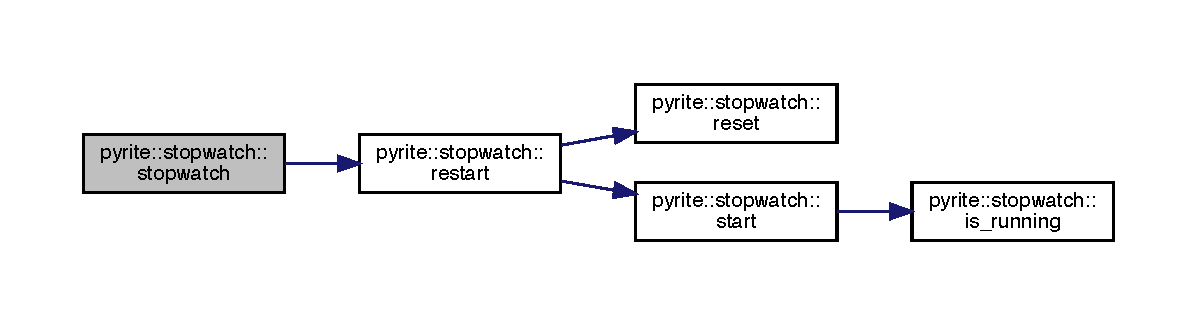
\includegraphics[width=350pt]{d6/dd1/classpyrite_1_1stopwatch_a685312010147a137543d0a65220153e6_cgraph}
\end{center}
\end{figure}
\mbox{\Hypertarget{classpyrite_1_1stopwatch_a5a833844590a54c1027b572fbef8dcb6}\label{classpyrite_1_1stopwatch_a5a833844590a54c1027b572fbef8dcb6}} 
\index{pyrite\+::stopwatch@{pyrite\+::stopwatch}!stopwatch@{stopwatch}}
\index{stopwatch@{stopwatch}!pyrite\+::stopwatch@{pyrite\+::stopwatch}}
\subsubsection{\texorpdfstring{stopwatch()}{stopwatch()}\hspace{0.1cm}{\footnotesize\ttfamily [2/3]}}
{\footnotesize\ttfamily pyrite\+::stopwatch\+::stopwatch (\begin{DoxyParamCaption}\item[{\mbox{\hyperlink{classpyrite_1_1stopwatch}{stopwatch}} const \&}]{ }\end{DoxyParamCaption})\hspace{0.3cm}{\ttfamily [default]}, {\ttfamily [noexcept]}}

Copy constructor. generated by the compiler. \mbox{\Hypertarget{classpyrite_1_1stopwatch_ab640070338c43dbde8c8d0471bd415d7}\label{classpyrite_1_1stopwatch_ab640070338c43dbde8c8d0471bd415d7}} 
\index{pyrite\+::stopwatch@{pyrite\+::stopwatch}!stopwatch@{stopwatch}}
\index{stopwatch@{stopwatch}!pyrite\+::stopwatch@{pyrite\+::stopwatch}}
\subsubsection{\texorpdfstring{stopwatch()}{stopwatch()}\hspace{0.1cm}{\footnotesize\ttfamily [3/3]}}
{\footnotesize\ttfamily pyrite\+::stopwatch\+::stopwatch (\begin{DoxyParamCaption}\item[{\mbox{\hyperlink{classpyrite_1_1stopwatch}{stopwatch}} \&\&}]{ }\end{DoxyParamCaption})\hspace{0.3cm}{\ttfamily [default]}, {\ttfamily [noexcept]}}

Move constructor. generated by the compiler. \mbox{\Hypertarget{classpyrite_1_1stopwatch_a6371ecaf8fe6d96fa39e477e3a82e7fc}\label{classpyrite_1_1stopwatch_a6371ecaf8fe6d96fa39e477e3a82e7fc}} 
\index{pyrite\+::stopwatch@{pyrite\+::stopwatch}!````~stopwatch@{$\sim$stopwatch}}
\index{````~stopwatch@{$\sim$stopwatch}!pyrite\+::stopwatch@{pyrite\+::stopwatch}}
\subsubsection{\texorpdfstring{$\sim$stopwatch()}{~stopwatch()}}
{\footnotesize\ttfamily pyrite\+::stopwatch\+::$\sim$stopwatch (\begin{DoxyParamCaption}{ }\end{DoxyParamCaption})\hspace{0.3cm}{\ttfamily [default]}}

Destructor. generated by the compiler. 

\subsection{Member Function Documentation}
\mbox{\Hypertarget{classpyrite_1_1stopwatch_a8032beb577019ab16594273aaaa97eb0}\label{classpyrite_1_1stopwatch_a8032beb577019ab16594273aaaa97eb0}} 
\index{pyrite\+::stopwatch@{pyrite\+::stopwatch}!elapsed@{elapsed}}
\index{elapsed@{elapsed}!pyrite\+::stopwatch@{pyrite\+::stopwatch}}
\subsubsection{\texorpdfstring{elapsed()}{elapsed()}}
{\footnotesize\ttfamily template$<$typename Duration $>$ \\
Duration\+::rep pyrite\+::stopwatch\+::elapsed (\begin{DoxyParamCaption}{ }\end{DoxyParamCaption}) const\hspace{0.3cm}{\ttfamily [inline]}, {\ttfamily [noexcept]}}

Get the total elapsed time. 
\begin{DoxyTemplParams}{Template Parameters}
{\em Duration} & Result type. \\
\hline
\end{DoxyTemplParams}
\begin{DoxyReturn}{Returns}
Total elapsed time. 
\end{DoxyReturn}
\mbox{\Hypertarget{classpyrite_1_1stopwatch_a4d5006e83d13f28295756506415aeb15}\label{classpyrite_1_1stopwatch_a4d5006e83d13f28295756506415aeb15}} 
\index{pyrite\+::stopwatch@{pyrite\+::stopwatch}!elapsed\+\_\+milliseconds@{elapsed\+\_\+milliseconds}}
\index{elapsed\+\_\+milliseconds@{elapsed\+\_\+milliseconds}!pyrite\+::stopwatch@{pyrite\+::stopwatch}}
\subsubsection{\texorpdfstring{elapsed\+\_\+milliseconds()}{elapsed\_milliseconds()}}
{\footnotesize\ttfamily template$<$typename T $>$ \\
T pyrite\+::stopwatch\+::elapsed\+\_\+milliseconds (\begin{DoxyParamCaption}{ }\end{DoxyParamCaption}) const\hspace{0.3cm}{\ttfamily [inline]}, {\ttfamily [noexcept]}}

Get total elapsed time milliseconds. 
\begin{DoxyTemplParams}{Template Parameters}
{\em T} & result type \\
\hline
\end{DoxyTemplParams}
\begin{DoxyReturn}{Returns}
Total elapsed time milliseconds. 
\end{DoxyReturn}
\mbox{\Hypertarget{classpyrite_1_1stopwatch_a2925d97a9c0ec2ae7b4ebbea0e15e5eb}\label{classpyrite_1_1stopwatch_a2925d97a9c0ec2ae7b4ebbea0e15e5eb}} 
\index{pyrite\+::stopwatch@{pyrite\+::stopwatch}!elapsed\+\_\+seconds@{elapsed\+\_\+seconds}}
\index{elapsed\+\_\+seconds@{elapsed\+\_\+seconds}!pyrite\+::stopwatch@{pyrite\+::stopwatch}}
\subsubsection{\texorpdfstring{elapsed\+\_\+seconds()}{elapsed\_seconds()}}
{\footnotesize\ttfamily template$<$typename T $>$ \\
T pyrite\+::stopwatch\+::elapsed\+\_\+seconds (\begin{DoxyParamCaption}{ }\end{DoxyParamCaption}) const\hspace{0.3cm}{\ttfamily [inline]}, {\ttfamily [noexcept]}}

Get total elapsed time seconds. 
\begin{DoxyTemplParams}{Template Parameters}
{\em T} & Result type \\
\hline
\end{DoxyTemplParams}
\begin{DoxyReturn}{Returns}
Total elapsed time seconds. 
\end{DoxyReturn}
\mbox{\Hypertarget{classpyrite_1_1stopwatch_add72890f54bc7554c32b9588ac761eed}\label{classpyrite_1_1stopwatch_add72890f54bc7554c32b9588ac761eed}} 
\index{pyrite\+::stopwatch@{pyrite\+::stopwatch}!is\+\_\+running@{is\+\_\+running}}
\index{is\+\_\+running@{is\+\_\+running}!pyrite\+::stopwatch@{pyrite\+::stopwatch}}
\subsubsection{\texorpdfstring{is\+\_\+running()}{is\_running()}}
{\footnotesize\ttfamily bool pyrite\+::stopwatch\+::is\+\_\+running (\begin{DoxyParamCaption}{ }\end{DoxyParamCaption}) const\hspace{0.3cm}{\ttfamily [inline]}, {\ttfamily [noexcept]}}

Indicating whether the stopwatch timer is running. Here is the caller graph for this function\+:
\nopagebreak
\begin{figure}[H]
\begin{center}
\leavevmode
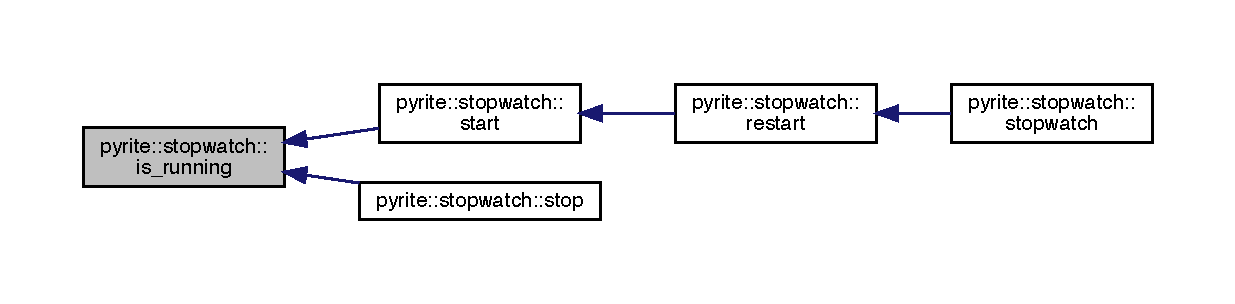
\includegraphics[width=350pt]{d6/dd1/classpyrite_1_1stopwatch_add72890f54bc7554c32b9588ac761eed_icgraph}
\end{center}
\end{figure}
\mbox{\Hypertarget{classpyrite_1_1stopwatch_a74042d6442db0cc278a76c6c548ed47b}\label{classpyrite_1_1stopwatch_a74042d6442db0cc278a76c6c548ed47b}} 
\index{pyrite\+::stopwatch@{pyrite\+::stopwatch}!operator=@{operator=}}
\index{operator=@{operator=}!pyrite\+::stopwatch@{pyrite\+::stopwatch}}
\subsubsection{\texorpdfstring{operator=()}{operator=()}\hspace{0.1cm}{\footnotesize\ttfamily [1/2]}}
{\footnotesize\ttfamily \mbox{\hyperlink{classpyrite_1_1stopwatch}{stopwatch}}\& pyrite\+::stopwatch\+::operator= (\begin{DoxyParamCaption}\item[{\mbox{\hyperlink{classpyrite_1_1stopwatch}{stopwatch}} const \&}]{ }\end{DoxyParamCaption})\hspace{0.3cm}{\ttfamily [default]}}

Copy assignment operator. generated by the compiler. \mbox{\Hypertarget{classpyrite_1_1stopwatch_a54c39e020d176c0e79d9726d44d41be2}\label{classpyrite_1_1stopwatch_a54c39e020d176c0e79d9726d44d41be2}} 
\index{pyrite\+::stopwatch@{pyrite\+::stopwatch}!operator=@{operator=}}
\index{operator=@{operator=}!pyrite\+::stopwatch@{pyrite\+::stopwatch}}
\subsubsection{\texorpdfstring{operator=()}{operator=()}\hspace{0.1cm}{\footnotesize\ttfamily [2/2]}}
{\footnotesize\ttfamily \mbox{\hyperlink{classpyrite_1_1stopwatch}{stopwatch}}\& pyrite\+::stopwatch\+::operator= (\begin{DoxyParamCaption}\item[{\mbox{\hyperlink{classpyrite_1_1stopwatch}{stopwatch}} \&\&}]{ }\end{DoxyParamCaption})\hspace{0.3cm}{\ttfamily [default]}}

Move assignment operator. generated by the compiler. \mbox{\Hypertarget{classpyrite_1_1stopwatch_ac6dd6a9c17ec2f2afc6b99cf1be86e04}\label{classpyrite_1_1stopwatch_ac6dd6a9c17ec2f2afc6b99cf1be86e04}} 
\index{pyrite\+::stopwatch@{pyrite\+::stopwatch}!reset@{reset}}
\index{reset@{reset}!pyrite\+::stopwatch@{pyrite\+::stopwatch}}
\subsubsection{\texorpdfstring{reset()}{reset()}}
{\footnotesize\ttfamily void pyrite\+::stopwatch\+::reset (\begin{DoxyParamCaption}{ }\end{DoxyParamCaption})\hspace{0.3cm}{\ttfamily [inline]}}

Stop time interval measurement and resets the elapsed time to zero. Here is the caller graph for this function\+:
\nopagebreak
\begin{figure}[H]
\begin{center}
\leavevmode
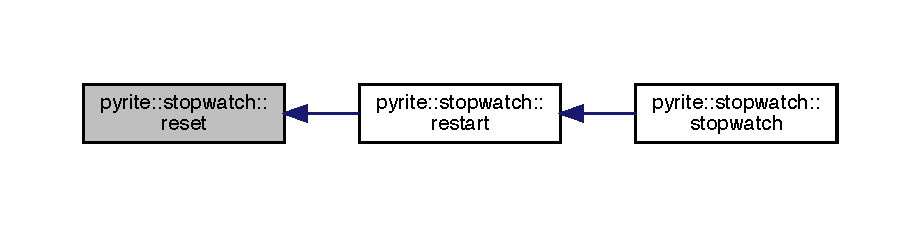
\includegraphics[width=350pt]{d6/dd1/classpyrite_1_1stopwatch_ac6dd6a9c17ec2f2afc6b99cf1be86e04_icgraph}
\end{center}
\end{figure}
\mbox{\Hypertarget{classpyrite_1_1stopwatch_a3fc39be2c2271eb57b9d8d30f5632dea}\label{classpyrite_1_1stopwatch_a3fc39be2c2271eb57b9d8d30f5632dea}} 
\index{pyrite\+::stopwatch@{pyrite\+::stopwatch}!restart@{restart}}
\index{restart@{restart}!pyrite\+::stopwatch@{pyrite\+::stopwatch}}
\subsubsection{\texorpdfstring{restart()}{restart()}}
{\footnotesize\ttfamily void pyrite\+::stopwatch\+::restart (\begin{DoxyParamCaption}{ }\end{DoxyParamCaption})\hspace{0.3cm}{\ttfamily [inline]}}

\mbox{\hyperlink{classpyrite_1_1stopwatch_ac6dd6a9c17ec2f2afc6b99cf1be86e04}{reset()}} and \mbox{\hyperlink{classpyrite_1_1stopwatch_ae1f6baec67daf518cf4d6bfbaab43cb1}{start()}} Here is the call graph for this function\+:
\nopagebreak
\begin{figure}[H]
\begin{center}
\leavevmode
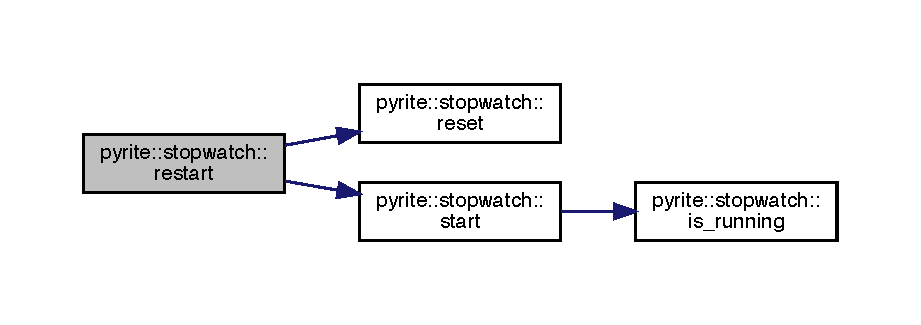
\includegraphics[width=350pt]{d6/dd1/classpyrite_1_1stopwatch_a3fc39be2c2271eb57b9d8d30f5632dea_cgraph}
\end{center}
\end{figure}
Here is the caller graph for this function\+:
\nopagebreak
\begin{figure}[H]
\begin{center}
\leavevmode
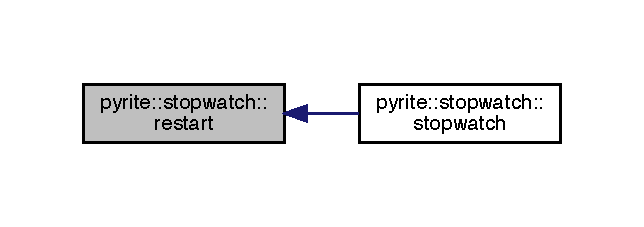
\includegraphics[width=309pt]{d6/dd1/classpyrite_1_1stopwatch_a3fc39be2c2271eb57b9d8d30f5632dea_icgraph}
\end{center}
\end{figure}
\mbox{\Hypertarget{classpyrite_1_1stopwatch_ae1f6baec67daf518cf4d6bfbaab43cb1}\label{classpyrite_1_1stopwatch_ae1f6baec67daf518cf4d6bfbaab43cb1}} 
\index{pyrite\+::stopwatch@{pyrite\+::stopwatch}!start@{start}}
\index{start@{start}!pyrite\+::stopwatch@{pyrite\+::stopwatch}}
\subsubsection{\texorpdfstring{start()}{start()}}
{\footnotesize\ttfamily void pyrite\+::stopwatch\+::start (\begin{DoxyParamCaption}{ }\end{DoxyParamCaption})\hspace{0.3cm}{\ttfamily [inline]}}

Starts, or resumes, measuring elapsed time for an interval. Here is the call graph for this function\+:
\nopagebreak
\begin{figure}[H]
\begin{center}
\leavevmode
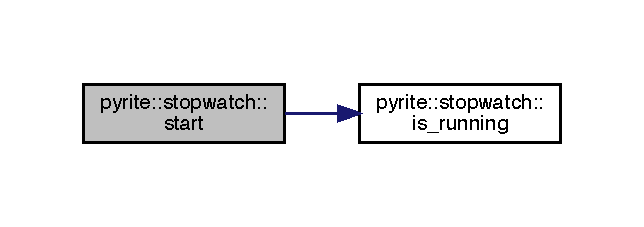
\includegraphics[width=309pt]{d6/dd1/classpyrite_1_1stopwatch_ae1f6baec67daf518cf4d6bfbaab43cb1_cgraph}
\end{center}
\end{figure}
Here is the caller graph for this function\+:
\nopagebreak
\begin{figure}[H]
\begin{center}
\leavevmode
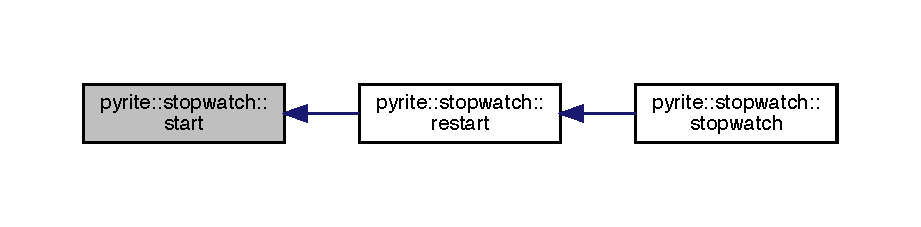
\includegraphics[width=350pt]{d6/dd1/classpyrite_1_1stopwatch_ae1f6baec67daf518cf4d6bfbaab43cb1_icgraph}
\end{center}
\end{figure}
\mbox{\Hypertarget{classpyrite_1_1stopwatch_acfacb195247f465f29cedaa9e8686e82}\label{classpyrite_1_1stopwatch_acfacb195247f465f29cedaa9e8686e82}} 
\index{pyrite\+::stopwatch@{pyrite\+::stopwatch}!stop@{stop}}
\index{stop@{stop}!pyrite\+::stopwatch@{pyrite\+::stopwatch}}
\subsubsection{\texorpdfstring{stop()}{stop()}}
{\footnotesize\ttfamily void pyrite\+::stopwatch\+::stop (\begin{DoxyParamCaption}{ }\end{DoxyParamCaption})\hspace{0.3cm}{\ttfamily [inline]}}

Stops measuring elapsed time for an interval. Here is the call graph for this function\+:
\nopagebreak
\begin{figure}[H]
\begin{center}
\leavevmode
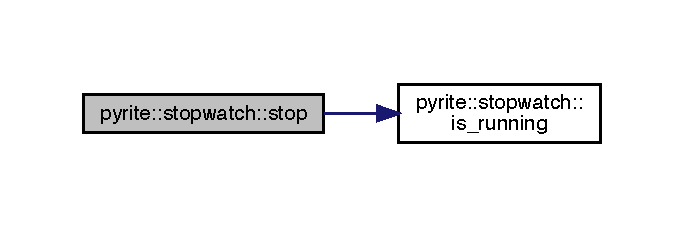
\includegraphics[width=328pt]{d6/dd1/classpyrite_1_1stopwatch_acfacb195247f465f29cedaa9e8686e82_cgraph}
\end{center}
\end{figure}


The documentation for this class was generated from the following file\+:\begin{DoxyCompactItemize}
\item 
/\+Users/masato.\+tanaka/\+Development/cpp/pyrite/pyrite/\mbox{\hyperlink{stopwatch_8hpp}{stopwatch.\+hpp}}\end{DoxyCompactItemize}

\hypertarget{structpyrite_1_1mpl_1_1tail}{}\section{pyrite\+:\+:mpl\+:\+:tail$<$ List $>$ Struct Template Reference}
\label{structpyrite_1_1mpl_1_1tail}\index{pyrite\+::mpl\+::tail$<$ List $>$@{pyrite\+::mpl\+::tail$<$ List $>$}}
\subsection*{Public Types}
\begin{DoxyCompactItemize}
\item 
\mbox{\Hypertarget{structpyrite_1_1mpl_1_1tail_a322a8b644102b0082116da1c6c88d84f}\label{structpyrite_1_1mpl_1_1tail_a322a8b644102b0082116da1c6c88d84f}} 
using {\bfseries type} = \mbox{\hyperlink{structpyrite_1_1core_1_1mpl_1_1type__list}{type\+\_\+list}}$<$$>$
\end{DoxyCompactItemize}


The documentation for this struct was generated from the following file\+:\begin{DoxyCompactItemize}
\item 
/\+Users/masato.\+tanaka/\+Development/cpp/pyrite/pyrite/mpl/type\+\_\+list/\mbox{\hyperlink{tail_8hpp}{tail.\+hpp}}\end{DoxyCompactItemize}

\hypertarget{structpyrite_1_1mpl_1_1tail_3_01type__list_3_01_head_00_01_tail_8_8_8_01_4_01_4}{}\section{pyrite\+:\+:mpl\+:\+:tail$<$ type\+\_\+list$<$ Head, Tail... $>$ $>$ Struct Template Reference}
\label{structpyrite_1_1mpl_1_1tail_3_01type__list_3_01_head_00_01_tail_8_8_8_01_4_01_4}\index{pyrite\+::mpl\+::tail$<$ type\+\_\+list$<$ Head, Tail... $>$ $>$@{pyrite\+::mpl\+::tail$<$ type\+\_\+list$<$ Head, Tail... $>$ $>$}}
\subsection*{Public Types}
\begin{DoxyCompactItemize}
\item 
\mbox{\Hypertarget{structpyrite_1_1mpl_1_1tail_3_01type__list_3_01_head_00_01_tail_8_8_8_01_4_01_4_a33fa4772cd6f330f68a17f9d6a1236d4}\label{structpyrite_1_1mpl_1_1tail_3_01type__list_3_01_head_00_01_tail_8_8_8_01_4_01_4_a33fa4772cd6f330f68a17f9d6a1236d4}} 
using {\bfseries type} = \mbox{\hyperlink{structpyrite_1_1core_1_1mpl_1_1type__list}{type\+\_\+list}}$<$ Tail... $>$
\end{DoxyCompactItemize}


The documentation for this struct was generated from the following file\+:\begin{DoxyCompactItemize}
\item 
/\+Users/masato.\+tanaka/\+Development/cpp/pyrite/pyrite/mpl/type\+\_\+list/\mbox{\hyperlink{tail_8hpp}{tail.\+hpp}}\end{DoxyCompactItemize}

\hypertarget{structpyrite_1_1mpl_1_1transform}{}\section{pyrite\+:\+:mpl\+:\+:transform$<$ List, F $>$ Struct Template Reference}
\label{structpyrite_1_1mpl_1_1transform}\index{pyrite\+::mpl\+::transform$<$ List, F $>$@{pyrite\+::mpl\+::transform$<$ List, F $>$}}


The documentation for this struct was generated from the following file\+:\begin{DoxyCompactItemize}
\item 
/\+Users/masato.\+tanaka/\+Development/cpp/pyrite/pyrite/mpl/type\+\_\+list/\mbox{\hyperlink{transform_8hpp}{transform.\+hpp}}\end{DoxyCompactItemize}

\hypertarget{structpyrite_1_1mpl_1_1transform_3_01type__list_3_01_t_8_8_8_01_4_00_01_f_01_4}{}\section{pyrite\+:\+:mpl\+:\+:transform$<$ type\+\_\+list$<$ T... $>$, F $>$ Struct Template Reference}
\label{structpyrite_1_1mpl_1_1transform_3_01type__list_3_01_t_8_8_8_01_4_00_01_f_01_4}\index{pyrite\+::mpl\+::transform$<$ type\+\_\+list$<$ T... $>$, F $>$@{pyrite\+::mpl\+::transform$<$ type\+\_\+list$<$ T... $>$, F $>$}}
\subsection*{Public Types}
\begin{DoxyCompactItemize}
\item 
\mbox{\Hypertarget{structpyrite_1_1mpl_1_1transform_3_01type__list_3_01_t_8_8_8_01_4_00_01_f_01_4_ad5ebc0efe3da4bd2f00fa1dcf161c4e7}\label{structpyrite_1_1mpl_1_1transform_3_01type__list_3_01_t_8_8_8_01_4_00_01_f_01_4_ad5ebc0efe3da4bd2f00fa1dcf161c4e7}} 
using {\bfseries type} = \mbox{\hyperlink{structpyrite_1_1core_1_1mpl_1_1type__list}{type\+\_\+list}}$<$ typename F$<$ T $>$\+::type... $>$
\end{DoxyCompactItemize}


The documentation for this struct was generated from the following file\+:\begin{DoxyCompactItemize}
\item 
/\+Users/masato.\+tanaka/\+Development/cpp/pyrite/pyrite/mpl/type\+\_\+list/\mbox{\hyperlink{transform_8hpp}{transform.\+hpp}}\end{DoxyCompactItemize}

\hypertarget{structpyrite_1_1core_1_1mpl_1_1type__list}{}\section{pyrite\+:\+:core\+:\+:mpl\+:\+:type\+\_\+list$<$ Args $>$ Struct Template Reference}
\label{structpyrite_1_1core_1_1mpl_1_1type__list}\index{pyrite\+::core\+::mpl\+::type\+\_\+list$<$ Args $>$@{pyrite\+::core\+::mpl\+::type\+\_\+list$<$ Args $>$}}
\subsection*{Public Types}
\begin{DoxyCompactItemize}
\item 
\mbox{\Hypertarget{structpyrite_1_1core_1_1mpl_1_1type__list_ae35eb4f4ab39374f2786c1b1b933327f}\label{structpyrite_1_1core_1_1mpl_1_1type__list_ae35eb4f4ab39374f2786c1b1b933327f}} 
using {\bfseries type} = \mbox{\hyperlink{structpyrite_1_1core_1_1mpl_1_1type__list}{type\+\_\+list}}$<$ Args... $>$
\end{DoxyCompactItemize}
\subsection*{Static Public Attributes}
\begin{DoxyCompactItemize}
\item 
\mbox{\Hypertarget{structpyrite_1_1core_1_1mpl_1_1type__list_a13b8657c429b51b70c2c41485d90801d}\label{structpyrite_1_1core_1_1mpl_1_1type__list_a13b8657c429b51b70c2c41485d90801d}} 
static constexpr std\+::size\+\_\+t {\bfseries size} = sizeof...(Args)
\end{DoxyCompactItemize}


The documentation for this struct was generated from the following file\+:\begin{DoxyCompactItemize}
\item 
/\+Users/masato.\+tanaka/\+Development/cpp/pyrite/pyrite/core/mpl/type\+\_\+list/\mbox{\hyperlink{core_2mpl_2type__list_2type__list_8hpp}{type\+\_\+list.\+hpp}}\end{DoxyCompactItemize}

\hypertarget{structpyrite_1_1core_1_1mpl_1_1type__optional}{}\section{pyrite\+:\+:core\+:\+:mpl\+:\+:type\+\_\+optional$<$ T $>$ Struct Template Reference}
\label{structpyrite_1_1core_1_1mpl_1_1type__optional}\index{pyrite\+::core\+::mpl\+::type\+\_\+optional$<$ T $>$@{pyrite\+::core\+::mpl\+::type\+\_\+optional$<$ T $>$}}


The documentation for this struct was generated from the following file\+:\begin{DoxyCompactItemize}
\item 
/\+Users/masato.\+tanaka/\+Development/cpp/pyrite/pyrite/core/mpl/\mbox{\hyperlink{core_2mpl_2type__optional_8hpp}{type\+\_\+optional.\+hpp}}\end{DoxyCompactItemize}

\hypertarget{structpyrite_1_1core_1_1mpl_1_1type__optional_3_01_t_01_4}{}\section{pyrite\+:\+:core\+:\+:mpl\+:\+:type\+\_\+optional$<$ T $>$ Struct Template Reference}
\label{structpyrite_1_1core_1_1mpl_1_1type__optional_3_01_t_01_4}\index{pyrite\+::core\+::mpl\+::type\+\_\+optional$<$ T $>$@{pyrite\+::core\+::mpl\+::type\+\_\+optional$<$ T $>$}}
\subsection*{Public Types}
\begin{DoxyCompactItemize}
\item 
\mbox{\Hypertarget{structpyrite_1_1core_1_1mpl_1_1type__optional_3_01_t_01_4_abdc68e65d67b41f0b623b91110b7ecfa}\label{structpyrite_1_1core_1_1mpl_1_1type__optional_3_01_t_01_4_abdc68e65d67b41f0b623b91110b7ecfa}} 
using {\bfseries type} = T
\item 
\mbox{\Hypertarget{structpyrite_1_1core_1_1mpl_1_1type__optional_3_01_t_01_4_ad67358168a5031ae600651471a040700}\label{structpyrite_1_1core_1_1mpl_1_1type__optional_3_01_t_01_4_ad67358168a5031ae600651471a040700}} 
{\footnotesize template$<$typename U $>$ }\\using {\bfseries type\+\_\+or} = T
\end{DoxyCompactItemize}
\subsection*{Static Public Attributes}
\begin{DoxyCompactItemize}
\item 
\mbox{\Hypertarget{structpyrite_1_1core_1_1mpl_1_1type__optional_3_01_t_01_4_ab4721d2101fded2df69667c35014f6d9}\label{structpyrite_1_1core_1_1mpl_1_1type__optional_3_01_t_01_4_ab4721d2101fded2df69667c35014f6d9}} 
static constexpr bool {\bfseries has\+\_\+type} = true
\end{DoxyCompactItemize}


The documentation for this struct was generated from the following file\+:\begin{DoxyCompactItemize}
\item 
/\+Users/masato.\+tanaka/\+Development/cpp/pyrite/pyrite/core/mpl/\mbox{\hyperlink{core_2mpl_2type__optional_8hpp}{type\+\_\+optional.\+hpp}}\end{DoxyCompactItemize}

\hypertarget{structpyrite_1_1core_1_1mpl_1_1type__optional_3_4}{}\section{pyrite\+:\+:core\+:\+:mpl\+:\+:type\+\_\+optional$<$$>$ Struct Template Reference}
\label{structpyrite_1_1core_1_1mpl_1_1type__optional_3_4}\index{pyrite\+::core\+::mpl\+::type\+\_\+optional$<$$>$@{pyrite\+::core\+::mpl\+::type\+\_\+optional$<$$>$}}
\subsection*{Public Types}
\begin{DoxyCompactItemize}
\item 
\mbox{\Hypertarget{structpyrite_1_1core_1_1mpl_1_1type__optional_3_4_a5297b69b30a8b7bfb8547c8105cae8b0}\label{structpyrite_1_1core_1_1mpl_1_1type__optional_3_4_a5297b69b30a8b7bfb8547c8105cae8b0}} 
{\footnotesize template$<$typename U $>$ }\\using {\bfseries type\+\_\+or} = U
\end{DoxyCompactItemize}
\subsection*{Static Public Attributes}
\begin{DoxyCompactItemize}
\item 
\mbox{\Hypertarget{structpyrite_1_1core_1_1mpl_1_1type__optional_3_4_a7d70f466faf93364ff1b7e0e0657d99a}\label{structpyrite_1_1core_1_1mpl_1_1type__optional_3_4_a7d70f466faf93364ff1b7e0e0657d99a}} 
static constexpr bool {\bfseries has\+\_\+type} = false
\end{DoxyCompactItemize}


The documentation for this struct was generated from the following file\+:\begin{DoxyCompactItemize}
\item 
/\+Users/masato.\+tanaka/\+Development/cpp/pyrite/pyrite/core/mpl/\mbox{\hyperlink{core_2mpl_2type__optional_8hpp}{type\+\_\+optional.\+hpp}}\end{DoxyCompactItemize}

\hypertarget{structpyrite_1_1mpl_1_1type__pair}{}\section{pyrite\+:\+:mpl\+:\+:type\+\_\+pair$<$ First, Second $>$ Struct Template Reference}
\label{structpyrite_1_1mpl_1_1type__pair}\index{pyrite\+::mpl\+::type\+\_\+pair$<$ First, Second $>$@{pyrite\+::mpl\+::type\+\_\+pair$<$ First, Second $>$}}
\subsection*{Public Types}
\begin{DoxyCompactItemize}
\item 
\mbox{\Hypertarget{structpyrite_1_1mpl_1_1type__pair_ab8c506211d061b54d06da4abb8f6bf32}\label{structpyrite_1_1mpl_1_1type__pair_ab8c506211d061b54d06da4abb8f6bf32}} 
using {\bfseries first} = First
\item 
\mbox{\Hypertarget{structpyrite_1_1mpl_1_1type__pair_a7f44105554b3a76114e982fe3ba247fa}\label{structpyrite_1_1mpl_1_1type__pair_a7f44105554b3a76114e982fe3ba247fa}} 
using {\bfseries second} = Second
\end{DoxyCompactItemize}


The documentation for this struct was generated from the following file\+:\begin{DoxyCompactItemize}
\item 
/\+Users/masato.\+tanaka/\+Development/cpp/pyrite/pyrite/mpl/type\+\_\+pair.\+hpp\end{DoxyCompactItemize}

\hypertarget{structpyrite_1_1math_1_1vector__traits}{}\section{pyrite\+:\+:math\+:\+:vector\+\_\+traits$<$ T $>$ Struct Template Reference}
\label{structpyrite_1_1math_1_1vector__traits}\index{pyrite\+::math\+::vector\+\_\+traits$<$ T $>$@{pyrite\+::math\+::vector\+\_\+traits$<$ T $>$}}


{\ttfamily \#include $<$vector\+\_\+traits.\+hpp$>$}

\subsection*{Public Types}
\begin{DoxyCompactItemize}
\item 
using \mbox{\hyperlink{structpyrite_1_1math_1_1vector__traits_abae24d3748d9ac5db627b6288822400f}{vector\+\_\+type}} = T
\item 
using \mbox{\hyperlink{structpyrite_1_1math_1_1vector__traits_a727892393454b3e72d96a1f3c15b37e2}{value\+\_\+type}} = typename T\+::value\+\_\+type
\end{DoxyCompactItemize}
\subsection*{Static Public Member Functions}
\begin{DoxyCompactItemize}
\item 
static constexpr \mbox{\hyperlink{structpyrite_1_1math_1_1vector__traits_a727892393454b3e72d96a1f3c15b37e2}{value\+\_\+type}} \& \mbox{\hyperlink{structpyrite_1_1math_1_1vector__traits_a4eb1d1180c18fd414ed2f080322f2533}{at}} (\mbox{\hyperlink{structpyrite_1_1math_1_1vector__traits_abae24d3748d9ac5db627b6288822400f}{vector\+\_\+type}} \&vector, \mbox{\hyperlink{type_8hpp_a3984e6dc0a53b867e054e8447f2f2be1}{usize}} const \&index)
\item 
static constexpr \mbox{\hyperlink{structpyrite_1_1math_1_1vector__traits_a727892393454b3e72d96a1f3c15b37e2}{value\+\_\+type}} const  \& \mbox{\hyperlink{structpyrite_1_1math_1_1vector__traits_af292435739fbef535f287c658525376b}{at}} (\mbox{\hyperlink{structpyrite_1_1math_1_1vector__traits_abae24d3748d9ac5db627b6288822400f}{vector\+\_\+type}} const \&vector, \mbox{\hyperlink{type_8hpp_a3984e6dc0a53b867e054e8447f2f2be1}{usize}} const \&index)
\end{DoxyCompactItemize}
\subsection*{Static Public Attributes}
\begin{DoxyCompactItemize}
\item 
static constexpr \mbox{\hyperlink{type_8hpp_a3984e6dc0a53b867e054e8447f2f2be1}{usize}} \mbox{\hyperlink{structpyrite_1_1math_1_1vector__traits_a79d22d82f3fc84d91df6128e70c61382}{dimension}} = T\+::dimension
\end{DoxyCompactItemize}


\subsection{Detailed Description}
\subsubsection*{template$<$typename T$>$\newline
struct pyrite\+::math\+::vector\+\_\+traits$<$ T $>$}

Traits for abstract access to vector type. 

\subsection{Member Typedef Documentation}
\mbox{\Hypertarget{structpyrite_1_1math_1_1vector__traits_a727892393454b3e72d96a1f3c15b37e2}\label{structpyrite_1_1math_1_1vector__traits_a727892393454b3e72d96a1f3c15b37e2}} 
\index{pyrite\+::math\+::vector\+\_\+traits@{pyrite\+::math\+::vector\+\_\+traits}!value\+\_\+type@{value\+\_\+type}}
\index{value\+\_\+type@{value\+\_\+type}!pyrite\+::math\+::vector\+\_\+traits@{pyrite\+::math\+::vector\+\_\+traits}}
\subsubsection{\texorpdfstring{value\+\_\+type}{value\_type}}
{\footnotesize\ttfamily template$<$typename T $>$ \\
using \mbox{\hyperlink{structpyrite_1_1math_1_1vector__traits}{pyrite\+::math\+::vector\+\_\+traits}}$<$ T $>$\+::\mbox{\hyperlink{structpyrite_1_1math_1_1vector__traits_a727892393454b3e72d96a1f3c15b37e2}{value\+\_\+type}} =  typename T\+::value\+\_\+type}

Element type of vector. \mbox{\Hypertarget{structpyrite_1_1math_1_1vector__traits_abae24d3748d9ac5db627b6288822400f}\label{structpyrite_1_1math_1_1vector__traits_abae24d3748d9ac5db627b6288822400f}} 
\index{pyrite\+::math\+::vector\+\_\+traits@{pyrite\+::math\+::vector\+\_\+traits}!vector\+\_\+type@{vector\+\_\+type}}
\index{vector\+\_\+type@{vector\+\_\+type}!pyrite\+::math\+::vector\+\_\+traits@{pyrite\+::math\+::vector\+\_\+traits}}
\subsubsection{\texorpdfstring{vector\+\_\+type}{vector\_type}}
{\footnotesize\ttfamily template$<$typename T $>$ \\
using \mbox{\hyperlink{structpyrite_1_1math_1_1vector__traits}{pyrite\+::math\+::vector\+\_\+traits}}$<$ T $>$\+::\mbox{\hyperlink{structpyrite_1_1math_1_1vector__traits_abae24d3748d9ac5db627b6288822400f}{vector\+\_\+type}} =  T}

The type of vector. 

\subsection{Member Function Documentation}
\mbox{\Hypertarget{structpyrite_1_1math_1_1vector__traits_a4eb1d1180c18fd414ed2f080322f2533}\label{structpyrite_1_1math_1_1vector__traits_a4eb1d1180c18fd414ed2f080322f2533}} 
\index{pyrite\+::math\+::vector\+\_\+traits@{pyrite\+::math\+::vector\+\_\+traits}!at@{at}}
\index{at@{at}!pyrite\+::math\+::vector\+\_\+traits@{pyrite\+::math\+::vector\+\_\+traits}}
\subsubsection{\texorpdfstring{at()}{at()}\hspace{0.1cm}{\footnotesize\ttfamily [1/2]}}
{\footnotesize\ttfamily template$<$typename T $>$ \\
static constexpr \mbox{\hyperlink{structpyrite_1_1math_1_1vector__traits_a727892393454b3e72d96a1f3c15b37e2}{value\+\_\+type}}\& \mbox{\hyperlink{structpyrite_1_1math_1_1vector__traits}{pyrite\+::math\+::vector\+\_\+traits}}$<$ T $>$\+::at (\begin{DoxyParamCaption}\item[{\mbox{\hyperlink{structpyrite_1_1math_1_1vector__traits_abae24d3748d9ac5db627b6288822400f}{vector\+\_\+type}} \&}]{vector,  }\item[{\mbox{\hyperlink{type_8hpp_a3984e6dc0a53b867e054e8447f2f2be1}{usize}} const \&}]{index }\end{DoxyParamCaption})\hspace{0.3cm}{\ttfamily [inline]}, {\ttfamily [static]}}

Access to elements of editable vector. 
\begin{DoxyParams}[1]{Parameters}
\mbox{\tt in}  & {\em vector} & vector \\
\hline
\mbox{\tt in}  & {\em index} & Index of vector. \\
\hline
\end{DoxyParams}
\begin{DoxyReturn}{Returns}
A reference to an element of an editable vector. 
\end{DoxyReturn}
\mbox{\Hypertarget{structpyrite_1_1math_1_1vector__traits_af292435739fbef535f287c658525376b}\label{structpyrite_1_1math_1_1vector__traits_af292435739fbef535f287c658525376b}} 
\index{pyrite\+::math\+::vector\+\_\+traits@{pyrite\+::math\+::vector\+\_\+traits}!at@{at}}
\index{at@{at}!pyrite\+::math\+::vector\+\_\+traits@{pyrite\+::math\+::vector\+\_\+traits}}
\subsubsection{\texorpdfstring{at()}{at()}\hspace{0.1cm}{\footnotesize\ttfamily [2/2]}}
{\footnotesize\ttfamily template$<$typename T $>$ \\
static constexpr \mbox{\hyperlink{structpyrite_1_1math_1_1vector__traits_a727892393454b3e72d96a1f3c15b37e2}{value\+\_\+type}} const\& \mbox{\hyperlink{structpyrite_1_1math_1_1vector__traits}{pyrite\+::math\+::vector\+\_\+traits}}$<$ T $>$\+::at (\begin{DoxyParamCaption}\item[{\mbox{\hyperlink{structpyrite_1_1math_1_1vector__traits_abae24d3748d9ac5db627b6288822400f}{vector\+\_\+type}} const \&}]{vector,  }\item[{\mbox{\hyperlink{type_8hpp_a3984e6dc0a53b867e054e8447f2f2be1}{usize}} const \&}]{index }\end{DoxyParamCaption})\hspace{0.3cm}{\ttfamily [inline]}, {\ttfamily [static]}}

Access to elements of uneditable vector. 
\begin{DoxyParams}[1]{Parameters}
\mbox{\tt in}  & {\em vector} & vector \\
\hline
\mbox{\tt in}  & {\em index} & Index of vector. \\
\hline
\end{DoxyParams}
\begin{DoxyReturn}{Returns}
A reference to an element of an uneditable vector. 
\end{DoxyReturn}


\subsection{Member Data Documentation}
\mbox{\Hypertarget{structpyrite_1_1math_1_1vector__traits_a79d22d82f3fc84d91df6128e70c61382}\label{structpyrite_1_1math_1_1vector__traits_a79d22d82f3fc84d91df6128e70c61382}} 
\index{pyrite\+::math\+::vector\+\_\+traits@{pyrite\+::math\+::vector\+\_\+traits}!dimension@{dimension}}
\index{dimension@{dimension}!pyrite\+::math\+::vector\+\_\+traits@{pyrite\+::math\+::vector\+\_\+traits}}
\subsubsection{\texorpdfstring{dimension}{dimension}}
{\footnotesize\ttfamily template$<$typename T $>$ \\
constexpr \mbox{\hyperlink{type_8hpp_a3984e6dc0a53b867e054e8447f2f2be1}{usize}} \mbox{\hyperlink{structpyrite_1_1math_1_1vector__traits}{pyrite\+::math\+::vector\+\_\+traits}}$<$ T $>$\+::dimension = T\+::dimension\hspace{0.3cm}{\ttfamily [static]}}

Dimension of vector. 

The documentation for this struct was generated from the following file\+:\begin{DoxyCompactItemize}
\item 
/\+Users/masato.\+tanaka/\+Development/cpp/pyrite/pyrite/math/\mbox{\hyperlink{vector__traits_8hpp}{vector\+\_\+traits.\+hpp}}\end{DoxyCompactItemize}

\hypertarget{structpyrite_1_1math_1_1vector__traits_3_01std_1_1array_3_01_t_00_01_n_01_4_01_4}{}\section{pyrite\+:\+:math\+:\+:vector\+\_\+traits$<$ std\+:\+:array$<$ T, N $>$ $>$ Struct Template Reference}
\label{structpyrite_1_1math_1_1vector__traits_3_01std_1_1array_3_01_t_00_01_n_01_4_01_4}\index{pyrite\+::math\+::vector\+\_\+traits$<$ std\+::array$<$ T, N $>$ $>$@{pyrite\+::math\+::vector\+\_\+traits$<$ std\+::array$<$ T, N $>$ $>$}}


{\ttfamily \#include $<$array.\+hpp$>$}

\subsection*{Public Types}
\begin{DoxyCompactItemize}
\item 
using \mbox{\hyperlink{structpyrite_1_1math_1_1vector__traits_3_01std_1_1array_3_01_t_00_01_n_01_4_01_4_ab56bcf2e100c6dc74210043b04d2e2e5}{vector\+\_\+type}} = std\+::array$<$ T, N $>$
\item 
using \mbox{\hyperlink{structpyrite_1_1math_1_1vector__traits_3_01std_1_1array_3_01_t_00_01_n_01_4_01_4_ac0670c23e2c162f7e82457937744950b}{value\+\_\+type}} = T
\end{DoxyCompactItemize}
\subsection*{Static Public Member Functions}
\begin{DoxyCompactItemize}
\item 
static constexpr \mbox{\hyperlink{structpyrite_1_1math_1_1vector__traits_3_01std_1_1array_3_01_t_00_01_n_01_4_01_4_ac0670c23e2c162f7e82457937744950b}{value\+\_\+type}} \& \mbox{\hyperlink{structpyrite_1_1math_1_1vector__traits_3_01std_1_1array_3_01_t_00_01_n_01_4_01_4_a1172afb4039475693603d89d211c9c6d}{at}} (\mbox{\hyperlink{structpyrite_1_1math_1_1vector__traits_3_01std_1_1array_3_01_t_00_01_n_01_4_01_4_ab56bcf2e100c6dc74210043b04d2e2e5}{vector\+\_\+type}} \&vector, \mbox{\hyperlink{type_8hpp_a3984e6dc0a53b867e054e8447f2f2be1}{usize}} const \&index)
\item 
static constexpr \mbox{\hyperlink{structpyrite_1_1math_1_1vector__traits_3_01std_1_1array_3_01_t_00_01_n_01_4_01_4_ac0670c23e2c162f7e82457937744950b}{value\+\_\+type}} const  \& \mbox{\hyperlink{structpyrite_1_1math_1_1vector__traits_3_01std_1_1array_3_01_t_00_01_n_01_4_01_4_a42f207b251670881132aeefb8688407a}{at}} (\mbox{\hyperlink{structpyrite_1_1math_1_1vector__traits_3_01std_1_1array_3_01_t_00_01_n_01_4_01_4_ab56bcf2e100c6dc74210043b04d2e2e5}{vector\+\_\+type}} const \&vector, \mbox{\hyperlink{type_8hpp_a3984e6dc0a53b867e054e8447f2f2be1}{usize}} const \&index)
\end{DoxyCompactItemize}
\subsection*{Static Public Attributes}
\begin{DoxyCompactItemize}
\item 
static constexpr \mbox{\hyperlink{type_8hpp_a3984e6dc0a53b867e054e8447f2f2be1}{usize}} \mbox{\hyperlink{structpyrite_1_1math_1_1vector__traits_3_01std_1_1array_3_01_t_00_01_n_01_4_01_4_ab1070748cd19aba5438d5637109c8a62}{dimension}} = N
\end{DoxyCompactItemize}


\subsection{Detailed Description}
\subsubsection*{template$<$typename T, std\+::size\+\_\+t N$>$\newline
struct pyrite\+::math\+::vector\+\_\+traits$<$ std\+::array$<$ T, N $>$ $>$}

Traits for abstract access to vector type. Specialization for std\+::array$<$\+T, N$>$. 

\subsection{Member Typedef Documentation}
\mbox{\Hypertarget{structpyrite_1_1math_1_1vector__traits_3_01std_1_1array_3_01_t_00_01_n_01_4_01_4_ac0670c23e2c162f7e82457937744950b}\label{structpyrite_1_1math_1_1vector__traits_3_01std_1_1array_3_01_t_00_01_n_01_4_01_4_ac0670c23e2c162f7e82457937744950b}} 
\index{pyrite\+::math\+::vector\+\_\+traits$<$ std\+::array$<$ T, N $>$ $>$@{pyrite\+::math\+::vector\+\_\+traits$<$ std\+::array$<$ T, N $>$ $>$}!value\+\_\+type@{value\+\_\+type}}
\index{value\+\_\+type@{value\+\_\+type}!pyrite\+::math\+::vector\+\_\+traits$<$ std\+::array$<$ T, N $>$ $>$@{pyrite\+::math\+::vector\+\_\+traits$<$ std\+::array$<$ T, N $>$ $>$}}
\subsubsection{\texorpdfstring{value\+\_\+type}{value\_type}}
{\footnotesize\ttfamily template$<$typename T , std\+::size\+\_\+t N$>$ \\
using \mbox{\hyperlink{structpyrite_1_1math_1_1vector__traits}{pyrite\+::math\+::vector\+\_\+traits}}$<$ std\+::array$<$ T, N $>$ $>$\+::\mbox{\hyperlink{structpyrite_1_1math_1_1vector__traits_3_01std_1_1array_3_01_t_00_01_n_01_4_01_4_ac0670c23e2c162f7e82457937744950b}{value\+\_\+type}} =  T}

Element type of vector. \mbox{\Hypertarget{structpyrite_1_1math_1_1vector__traits_3_01std_1_1array_3_01_t_00_01_n_01_4_01_4_ab56bcf2e100c6dc74210043b04d2e2e5}\label{structpyrite_1_1math_1_1vector__traits_3_01std_1_1array_3_01_t_00_01_n_01_4_01_4_ab56bcf2e100c6dc74210043b04d2e2e5}} 
\index{pyrite\+::math\+::vector\+\_\+traits$<$ std\+::array$<$ T, N $>$ $>$@{pyrite\+::math\+::vector\+\_\+traits$<$ std\+::array$<$ T, N $>$ $>$}!vector\+\_\+type@{vector\+\_\+type}}
\index{vector\+\_\+type@{vector\+\_\+type}!pyrite\+::math\+::vector\+\_\+traits$<$ std\+::array$<$ T, N $>$ $>$@{pyrite\+::math\+::vector\+\_\+traits$<$ std\+::array$<$ T, N $>$ $>$}}
\subsubsection{\texorpdfstring{vector\+\_\+type}{vector\_type}}
{\footnotesize\ttfamily template$<$typename T , std\+::size\+\_\+t N$>$ \\
using \mbox{\hyperlink{structpyrite_1_1math_1_1vector__traits}{pyrite\+::math\+::vector\+\_\+traits}}$<$ std\+::array$<$ T, N $>$ $>$\+::\mbox{\hyperlink{structpyrite_1_1math_1_1vector__traits_3_01std_1_1array_3_01_t_00_01_n_01_4_01_4_ab56bcf2e100c6dc74210043b04d2e2e5}{vector\+\_\+type}} =  std\+::array$<$T, N$>$}

The type of vector. 

\subsection{Member Function Documentation}
\mbox{\Hypertarget{structpyrite_1_1math_1_1vector__traits_3_01std_1_1array_3_01_t_00_01_n_01_4_01_4_a1172afb4039475693603d89d211c9c6d}\label{structpyrite_1_1math_1_1vector__traits_3_01std_1_1array_3_01_t_00_01_n_01_4_01_4_a1172afb4039475693603d89d211c9c6d}} 
\index{pyrite\+::math\+::vector\+\_\+traits$<$ std\+::array$<$ T, N $>$ $>$@{pyrite\+::math\+::vector\+\_\+traits$<$ std\+::array$<$ T, N $>$ $>$}!at@{at}}
\index{at@{at}!pyrite\+::math\+::vector\+\_\+traits$<$ std\+::array$<$ T, N $>$ $>$@{pyrite\+::math\+::vector\+\_\+traits$<$ std\+::array$<$ T, N $>$ $>$}}
\subsubsection{\texorpdfstring{at()}{at()}\hspace{0.1cm}{\footnotesize\ttfamily [1/2]}}
{\footnotesize\ttfamily template$<$typename T , std\+::size\+\_\+t N$>$ \\
static constexpr \mbox{\hyperlink{structpyrite_1_1math_1_1vector__traits_3_01std_1_1array_3_01_t_00_01_n_01_4_01_4_ac0670c23e2c162f7e82457937744950b}{value\+\_\+type}}\& \mbox{\hyperlink{structpyrite_1_1math_1_1vector__traits}{pyrite\+::math\+::vector\+\_\+traits}}$<$ std\+::array$<$ T, N $>$ $>$\+::at (\begin{DoxyParamCaption}\item[{\mbox{\hyperlink{structpyrite_1_1math_1_1vector__traits_3_01std_1_1array_3_01_t_00_01_n_01_4_01_4_ab56bcf2e100c6dc74210043b04d2e2e5}{vector\+\_\+type}} \&}]{vector,  }\item[{\mbox{\hyperlink{type_8hpp_a3984e6dc0a53b867e054e8447f2f2be1}{usize}} const \&}]{index }\end{DoxyParamCaption})\hspace{0.3cm}{\ttfamily [inline]}, {\ttfamily [static]}}

Access to elements of editable vector. 
\begin{DoxyParams}[1]{Parameters}
\mbox{\tt in}  & {\em vector} & vector \\
\hline
\mbox{\tt in}  & {\em index} & Index of vector. \\
\hline
\end{DoxyParams}
\begin{DoxyReturn}{Returns}
A reference to an element of an editable vector. 
\end{DoxyReturn}
\mbox{\Hypertarget{structpyrite_1_1math_1_1vector__traits_3_01std_1_1array_3_01_t_00_01_n_01_4_01_4_a42f207b251670881132aeefb8688407a}\label{structpyrite_1_1math_1_1vector__traits_3_01std_1_1array_3_01_t_00_01_n_01_4_01_4_a42f207b251670881132aeefb8688407a}} 
\index{pyrite\+::math\+::vector\+\_\+traits$<$ std\+::array$<$ T, N $>$ $>$@{pyrite\+::math\+::vector\+\_\+traits$<$ std\+::array$<$ T, N $>$ $>$}!at@{at}}
\index{at@{at}!pyrite\+::math\+::vector\+\_\+traits$<$ std\+::array$<$ T, N $>$ $>$@{pyrite\+::math\+::vector\+\_\+traits$<$ std\+::array$<$ T, N $>$ $>$}}
\subsubsection{\texorpdfstring{at()}{at()}\hspace{0.1cm}{\footnotesize\ttfamily [2/2]}}
{\footnotesize\ttfamily template$<$typename T , std\+::size\+\_\+t N$>$ \\
static constexpr \mbox{\hyperlink{structpyrite_1_1math_1_1vector__traits_3_01std_1_1array_3_01_t_00_01_n_01_4_01_4_ac0670c23e2c162f7e82457937744950b}{value\+\_\+type}} const\& \mbox{\hyperlink{structpyrite_1_1math_1_1vector__traits}{pyrite\+::math\+::vector\+\_\+traits}}$<$ std\+::array$<$ T, N $>$ $>$\+::at (\begin{DoxyParamCaption}\item[{\mbox{\hyperlink{structpyrite_1_1math_1_1vector__traits_3_01std_1_1array_3_01_t_00_01_n_01_4_01_4_ab56bcf2e100c6dc74210043b04d2e2e5}{vector\+\_\+type}} const \&}]{vector,  }\item[{\mbox{\hyperlink{type_8hpp_a3984e6dc0a53b867e054e8447f2f2be1}{usize}} const \&}]{index }\end{DoxyParamCaption})\hspace{0.3cm}{\ttfamily [inline]}, {\ttfamily [static]}}

Access to elements of uneditable vector. 
\begin{DoxyParams}[1]{Parameters}
\mbox{\tt in}  & {\em vector} & vector \\
\hline
\mbox{\tt in}  & {\em index} & Index of vector. \\
\hline
\end{DoxyParams}
\begin{DoxyReturn}{Returns}
A reference to an element of an uneditable vector. 
\end{DoxyReturn}


\subsection{Member Data Documentation}
\mbox{\Hypertarget{structpyrite_1_1math_1_1vector__traits_3_01std_1_1array_3_01_t_00_01_n_01_4_01_4_ab1070748cd19aba5438d5637109c8a62}\label{structpyrite_1_1math_1_1vector__traits_3_01std_1_1array_3_01_t_00_01_n_01_4_01_4_ab1070748cd19aba5438d5637109c8a62}} 
\index{pyrite\+::math\+::vector\+\_\+traits$<$ std\+::array$<$ T, N $>$ $>$@{pyrite\+::math\+::vector\+\_\+traits$<$ std\+::array$<$ T, N $>$ $>$}!dimension@{dimension}}
\index{dimension@{dimension}!pyrite\+::math\+::vector\+\_\+traits$<$ std\+::array$<$ T, N $>$ $>$@{pyrite\+::math\+::vector\+\_\+traits$<$ std\+::array$<$ T, N $>$ $>$}}
\subsubsection{\texorpdfstring{dimension}{dimension}}
{\footnotesize\ttfamily template$<$typename T , std\+::size\+\_\+t N$>$ \\
constexpr \mbox{\hyperlink{type_8hpp_a3984e6dc0a53b867e054e8447f2f2be1}{usize}} \mbox{\hyperlink{structpyrite_1_1math_1_1vector__traits}{pyrite\+::math\+::vector\+\_\+traits}}$<$ std\+::array$<$ T, N $>$ $>$\+::dimension = N\hspace{0.3cm}{\ttfamily [static]}}

Dimension of vector. 

The documentation for this struct was generated from the following file\+:\begin{DoxyCompactItemize}
\item 
/\+Users/masato.\+tanaka/\+Development/cpp/pyrite/pyrite/math/vector\+\_\+traits/\mbox{\hyperlink{array_8hpp}{array.\+hpp}}\end{DoxyCompactItemize}

\hypertarget{structpyrite_1_1math_1_1vector__traits_3_01_t[_n]_4}{}\section{pyrite\+:\+:math\+:\+:vector\+\_\+traits$<$ T\mbox{[}N\mbox{]}$>$ Struct Template Reference}
\label{structpyrite_1_1math_1_1vector__traits_3_01_t[_n]_4}\index{pyrite\+::math\+::vector\+\_\+traits$<$ T\mbox{[}N\mbox{]}$>$@{pyrite\+::math\+::vector\+\_\+traits$<$ T[N]$>$}}


{\ttfamily \#include $<$array.\+hpp$>$}

\subsection*{Public Types}
\begin{DoxyCompactItemize}
\item 
using \mbox{\hyperlink{structpyrite_1_1math_1_1vector__traits_3_01_t[_n]_4_a092357eae264b1a7aaf1a6e66e41fb52}{vector\+\_\+type}} = T\mbox{[}N\mbox{]}
\item 
using \mbox{\hyperlink{structpyrite_1_1math_1_1vector__traits_3_01_t[_n]_4_ab6b98499d39e4fb65ea3addf98fd7960}{value\+\_\+type}} = T
\end{DoxyCompactItemize}
\subsection*{Static Public Member Functions}
\begin{DoxyCompactItemize}
\item 
static constexpr \mbox{\hyperlink{structpyrite_1_1math_1_1vector__traits_3_01_t[_n]_4_ab6b98499d39e4fb65ea3addf98fd7960}{value\+\_\+type}} \& \mbox{\hyperlink{structpyrite_1_1math_1_1vector__traits_3_01_t[_n]_4_a348aa9a8c63771e16d5e7637839f5b18}{at}} (\mbox{\hyperlink{structpyrite_1_1math_1_1vector__traits_3_01_t[_n]_4_a092357eae264b1a7aaf1a6e66e41fb52}{vector\+\_\+type}} \&vector, \mbox{\hyperlink{type_8hpp_a3984e6dc0a53b867e054e8447f2f2be1}{usize}} const \&index)
\item 
static constexpr \mbox{\hyperlink{structpyrite_1_1math_1_1vector__traits_3_01_t[_n]_4_ab6b98499d39e4fb65ea3addf98fd7960}{value\+\_\+type}} const  \& \mbox{\hyperlink{structpyrite_1_1math_1_1vector__traits_3_01_t[_n]_4_ab20211c2d98e264b1edfdb3f72b128a1}{at}} (\mbox{\hyperlink{structpyrite_1_1math_1_1vector__traits_3_01_t[_n]_4_a092357eae264b1a7aaf1a6e66e41fb52}{vector\+\_\+type}} const \&vector, \mbox{\hyperlink{type_8hpp_a3984e6dc0a53b867e054e8447f2f2be1}{usize}} const \&index)
\end{DoxyCompactItemize}
\subsection*{Static Public Attributes}
\begin{DoxyCompactItemize}
\item 
static constexpr \mbox{\hyperlink{type_8hpp_a3984e6dc0a53b867e054e8447f2f2be1}{usize}} \mbox{\hyperlink{structpyrite_1_1math_1_1vector__traits_3_01_t[_n]_4_a7afc072ea1bfd989f6b383a1a6cb788b}{dimension}} = N
\end{DoxyCompactItemize}


\subsection{Detailed Description}
\subsubsection*{template$<$typename T, std\+::size\+\_\+t N$>$\newline
struct pyrite\+::math\+::vector\+\_\+traits$<$ T\mbox{[}\+N\mbox{]}$>$}

Traits for abstract access to vector type. Specialization for embedded array. 

\subsection{Member Typedef Documentation}
\mbox{\Hypertarget{structpyrite_1_1math_1_1vector__traits_3_01_t[_n]_4_ab6b98499d39e4fb65ea3addf98fd7960}\label{structpyrite_1_1math_1_1vector__traits_3_01_t[_n]_4_ab6b98499d39e4fb65ea3addf98fd7960}} 
\index{pyrite\+::math\+::vector\+\_\+traits$<$ T\mbox{[}N\mbox{]}$>$@{pyrite\+::math\+::vector\+\_\+traits$<$ T[N]$>$}!value\+\_\+type@{value\+\_\+type}}
\index{value\+\_\+type@{value\+\_\+type}!pyrite\+::math\+::vector\+\_\+traits$<$ T\mbox{[}N\mbox{]}$>$@{pyrite\+::math\+::vector\+\_\+traits$<$ T[N]$>$}}
\subsubsection{\texorpdfstring{value\+\_\+type}{value\_type}}
{\footnotesize\ttfamily template$<$typename T , std\+::size\+\_\+t N$>$ \\
using \mbox{\hyperlink{structpyrite_1_1math_1_1vector__traits}{pyrite\+::math\+::vector\+\_\+traits}}$<$ T\mbox{[}N\mbox{]}$>$\+::\mbox{\hyperlink{structpyrite_1_1math_1_1vector__traits_3_01_t[_n]_4_ab6b98499d39e4fb65ea3addf98fd7960}{value\+\_\+type}} =  T}

Element type of vector. \mbox{\Hypertarget{structpyrite_1_1math_1_1vector__traits_3_01_t[_n]_4_a092357eae264b1a7aaf1a6e66e41fb52}\label{structpyrite_1_1math_1_1vector__traits_3_01_t[_n]_4_a092357eae264b1a7aaf1a6e66e41fb52}} 
\index{pyrite\+::math\+::vector\+\_\+traits$<$ T\mbox{[}N\mbox{]}$>$@{pyrite\+::math\+::vector\+\_\+traits$<$ T[N]$>$}!vector\+\_\+type@{vector\+\_\+type}}
\index{vector\+\_\+type@{vector\+\_\+type}!pyrite\+::math\+::vector\+\_\+traits$<$ T\mbox{[}N\mbox{]}$>$@{pyrite\+::math\+::vector\+\_\+traits$<$ T[N]$>$}}
\subsubsection{\texorpdfstring{vector\+\_\+type}{vector\_type}}
{\footnotesize\ttfamily template$<$typename T , std\+::size\+\_\+t N$>$ \\
using \mbox{\hyperlink{structpyrite_1_1math_1_1vector__traits}{pyrite\+::math\+::vector\+\_\+traits}}$<$ T\mbox{[}N\mbox{]}$>$\+::\mbox{\hyperlink{structpyrite_1_1math_1_1vector__traits_3_01_t[_n]_4_a092357eae264b1a7aaf1a6e66e41fb52}{vector\+\_\+type}} =  T\mbox{[}N\mbox{]}}

The type of vector. 

\subsection{Member Function Documentation}
\mbox{\Hypertarget{structpyrite_1_1math_1_1vector__traits_3_01_t[_n]_4_a348aa9a8c63771e16d5e7637839f5b18}\label{structpyrite_1_1math_1_1vector__traits_3_01_t[_n]_4_a348aa9a8c63771e16d5e7637839f5b18}} 
\index{pyrite\+::math\+::vector\+\_\+traits$<$ T\mbox{[}N\mbox{]}$>$@{pyrite\+::math\+::vector\+\_\+traits$<$ T[N]$>$}!at@{at}}
\index{at@{at}!pyrite\+::math\+::vector\+\_\+traits$<$ T\mbox{[}N\mbox{]}$>$@{pyrite\+::math\+::vector\+\_\+traits$<$ T[N]$>$}}
\subsubsection{\texorpdfstring{at()}{at()}\hspace{0.1cm}{\footnotesize\ttfamily [1/2]}}
{\footnotesize\ttfamily template$<$typename T , std\+::size\+\_\+t N$>$ \\
static constexpr \mbox{\hyperlink{structpyrite_1_1math_1_1vector__traits_3_01_t[_n]_4_ab6b98499d39e4fb65ea3addf98fd7960}{value\+\_\+type}}\& \mbox{\hyperlink{structpyrite_1_1math_1_1vector__traits}{pyrite\+::math\+::vector\+\_\+traits}}$<$ T\mbox{[}N\mbox{]}$>$\+::at (\begin{DoxyParamCaption}\item[{\mbox{\hyperlink{structpyrite_1_1math_1_1vector__traits_3_01_t[_n]_4_a092357eae264b1a7aaf1a6e66e41fb52}{vector\+\_\+type}} \&}]{vector,  }\item[{\mbox{\hyperlink{type_8hpp_a3984e6dc0a53b867e054e8447f2f2be1}{usize}} const \&}]{index }\end{DoxyParamCaption})\hspace{0.3cm}{\ttfamily [inline]}, {\ttfamily [static]}}

Access to elements of editable vector. 
\begin{DoxyParams}[1]{Parameters}
\mbox{\tt in}  & {\em vector} & vector \\
\hline
\mbox{\tt in}  & {\em index} & Index of vector. \\
\hline
\end{DoxyParams}
\begin{DoxyReturn}{Returns}
A reference to an element of an editable vector. 
\end{DoxyReturn}
\mbox{\Hypertarget{structpyrite_1_1math_1_1vector__traits_3_01_t[_n]_4_ab20211c2d98e264b1edfdb3f72b128a1}\label{structpyrite_1_1math_1_1vector__traits_3_01_t[_n]_4_ab20211c2d98e264b1edfdb3f72b128a1}} 
\index{pyrite\+::math\+::vector\+\_\+traits$<$ T\mbox{[}N\mbox{]}$>$@{pyrite\+::math\+::vector\+\_\+traits$<$ T[N]$>$}!at@{at}}
\index{at@{at}!pyrite\+::math\+::vector\+\_\+traits$<$ T\mbox{[}N\mbox{]}$>$@{pyrite\+::math\+::vector\+\_\+traits$<$ T[N]$>$}}
\subsubsection{\texorpdfstring{at()}{at()}\hspace{0.1cm}{\footnotesize\ttfamily [2/2]}}
{\footnotesize\ttfamily template$<$typename T , std\+::size\+\_\+t N$>$ \\
static constexpr \mbox{\hyperlink{structpyrite_1_1math_1_1vector__traits_3_01_t[_n]_4_ab6b98499d39e4fb65ea3addf98fd7960}{value\+\_\+type}} const\& \mbox{\hyperlink{structpyrite_1_1math_1_1vector__traits}{pyrite\+::math\+::vector\+\_\+traits}}$<$ T\mbox{[}N\mbox{]}$>$\+::at (\begin{DoxyParamCaption}\item[{\mbox{\hyperlink{structpyrite_1_1math_1_1vector__traits_3_01_t[_n]_4_a092357eae264b1a7aaf1a6e66e41fb52}{vector\+\_\+type}} const \&}]{vector,  }\item[{\mbox{\hyperlink{type_8hpp_a3984e6dc0a53b867e054e8447f2f2be1}{usize}} const \&}]{index }\end{DoxyParamCaption})\hspace{0.3cm}{\ttfamily [inline]}, {\ttfamily [static]}}

Access to elements of uneditable vector. 
\begin{DoxyParams}[1]{Parameters}
\mbox{\tt in}  & {\em vector} & vector \\
\hline
\mbox{\tt in}  & {\em index} & Index of vector. \\
\hline
\end{DoxyParams}
\begin{DoxyReturn}{Returns}
A reference to an element of an uneditable vector. 
\end{DoxyReturn}


\subsection{Member Data Documentation}
\mbox{\Hypertarget{structpyrite_1_1math_1_1vector__traits_3_01_t[_n]_4_a7afc072ea1bfd989f6b383a1a6cb788b}\label{structpyrite_1_1math_1_1vector__traits_3_01_t[_n]_4_a7afc072ea1bfd989f6b383a1a6cb788b}} 
\index{pyrite\+::math\+::vector\+\_\+traits$<$ T\mbox{[}N\mbox{]}$>$@{pyrite\+::math\+::vector\+\_\+traits$<$ T[N]$>$}!dimension@{dimension}}
\index{dimension@{dimension}!pyrite\+::math\+::vector\+\_\+traits$<$ T\mbox{[}N\mbox{]}$>$@{pyrite\+::math\+::vector\+\_\+traits$<$ T[N]$>$}}
\subsubsection{\texorpdfstring{dimension}{dimension}}
{\footnotesize\ttfamily template$<$typename T , std\+::size\+\_\+t N$>$ \\
constexpr \mbox{\hyperlink{type_8hpp_a3984e6dc0a53b867e054e8447f2f2be1}{usize}} \mbox{\hyperlink{structpyrite_1_1math_1_1vector__traits}{pyrite\+::math\+::vector\+\_\+traits}}$<$ T\mbox{[}N\mbox{]}$>$\+::dimension = N\hspace{0.3cm}{\ttfamily [static]}}

Dimension of vector. 

The documentation for this struct was generated from the following file\+:\begin{DoxyCompactItemize}
\item 
/\+Users/masato.\+tanaka/\+Development/cpp/pyrite/pyrite/math/vector\+\_\+traits/\mbox{\hyperlink{array_8hpp}{array.\+hpp}}\end{DoxyCompactItemize}

\hypertarget{structpyrite_1_1mpl_1_1zip}{}\section{pyrite\+:\+:mpl\+:\+:zip$<$ ListL, ListR $>$ Struct Template Reference}
\label{structpyrite_1_1mpl_1_1zip}\index{pyrite\+::mpl\+::zip$<$ List\+L, List\+R $>$@{pyrite\+::mpl\+::zip$<$ List\+L, List\+R $>$}}


The documentation for this struct was generated from the following file\+:\begin{DoxyCompactItemize}
\item 
/\+Users/masato.\+tanaka/\+Development/cpp/pyrite/pyrite/mpl/type\+\_\+list/\mbox{\hyperlink{zip_8hpp}{zip.\+hpp}}\end{DoxyCompactItemize}

\hypertarget{structpyrite_1_1mpl_1_1zip_3_01type__list_3_01_l_8_8_8_01_4_00_01type__list_3_01_r_8_8_8_01_4_01_4}{}\section{pyrite\+:\+:mpl\+:\+:zip$<$ type\+\_\+list$<$ L... $>$, type\+\_\+list$<$ R... $>$ $>$ Struct Template Reference}
\label{structpyrite_1_1mpl_1_1zip_3_01type__list_3_01_l_8_8_8_01_4_00_01type__list_3_01_r_8_8_8_01_4_01_4}\index{pyrite\+::mpl\+::zip$<$ type\+\_\+list$<$ L... $>$, type\+\_\+list$<$ R... $>$ $>$@{pyrite\+::mpl\+::zip$<$ type\+\_\+list$<$ L... $>$, type\+\_\+list$<$ R... $>$ $>$}}
\subsection*{Public Types}
\begin{DoxyCompactItemize}
\item 
\mbox{\Hypertarget{structpyrite_1_1mpl_1_1zip_3_01type__list_3_01_l_8_8_8_01_4_00_01type__list_3_01_r_8_8_8_01_4_01_4_a78da1b0b028f603038e6d67412e03c9a}\label{structpyrite_1_1mpl_1_1zip_3_01type__list_3_01_l_8_8_8_01_4_00_01type__list_3_01_r_8_8_8_01_4_01_4_a78da1b0b028f603038e6d67412e03c9a}} 
using {\bfseries type} = \mbox{\hyperlink{structpyrite_1_1core_1_1mpl_1_1type__list}{type\+\_\+list}}$<$ \mbox{\hyperlink{structpyrite_1_1mpl_1_1type__pair}{type\+\_\+pair}}$<$ L, R $>$... $>$
\end{DoxyCompactItemize}


The documentation for this struct was generated from the following file\+:\begin{DoxyCompactItemize}
\item 
/\+Users/masato.\+tanaka/\+Development/cpp/pyrite/pyrite/mpl/type\+\_\+list/\mbox{\hyperlink{zip_8hpp}{zip.\+hpp}}\end{DoxyCompactItemize}

\chapter{File Documentation}
\hypertarget{checked__delete_8hpp}{}\section{/\+Users/masato.tanaka/\+Development/cpp/pyrite/pyrite/core/checked\+\_\+delete.hpp File Reference}
\label{checked__delete_8hpp}\index{/\+Users/masato.\+tanaka/\+Development/cpp/pyrite/pyrite/core/checked\+\_\+delete.\+hpp@{/\+Users/masato.\+tanaka/\+Development/cpp/pyrite/pyrite/core/checked\+\_\+delete.\+hpp}}
{\ttfamily \#include $<$pyrite/core/is\+\_\+complete\+\_\+type.\+hpp$>$}\newline
Include dependency graph for checked\+\_\+delete.\+hpp\+:
\nopagebreak
\begin{figure}[H]
\begin{center}
\leavevmode
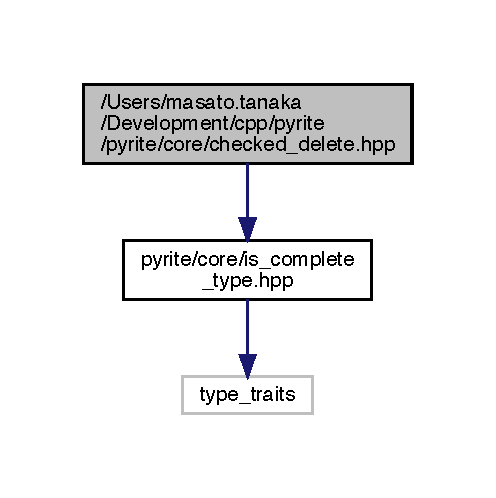
\includegraphics[width=238pt]{d0/d32/checked__delete_8hpp__incl}
\end{center}
\end{figure}
This graph shows which files directly or indirectly include this file\+:
\nopagebreak
\begin{figure}[H]
\begin{center}
\leavevmode
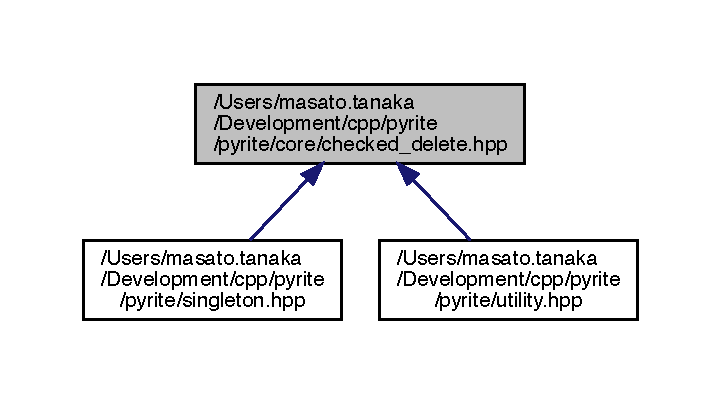
\includegraphics[width=346pt]{de/d3e/checked__delete_8hpp__dep__incl}
\end{center}
\end{figure}
\subsection*{Classes}
\begin{DoxyCompactItemize}
\item 
class \mbox{\hyperlink{classpyrite_1_1core_1_1checked__deleter}{pyrite\+::core\+::checked\+\_\+deleter$<$ T $>$}}
\item 
class \mbox{\hyperlink{classpyrite_1_1core_1_1checked__array__deleter}{pyrite\+::core\+::checked\+\_\+array\+\_\+deleter$<$ T $>$}}
\end{DoxyCompactItemize}
\subsection*{Functions}
\begin{DoxyCompactItemize}
\item 
{\footnotesize template$<$typename T $>$ }\\void \mbox{\hyperlink{checked__delete_8hpp_a27af49b4f86442c78de48cda0818eb72}{pyrite\+::core\+::checked\+\_\+delete}} (T $\ast$\&ptr)
\item 
{\footnotesize template$<$typename T $>$ }\\void \mbox{\hyperlink{checked__delete_8hpp_a47e9f6f9578e0518074ca6da633d7ea8}{pyrite\+::core\+::checked\+\_\+array\+\_\+delete}} (T $\ast$\&ptr)
\end{DoxyCompactItemize}


\subsection{Detailed Description}
\begin{DoxyAuthor}{Author}
block 
\end{DoxyAuthor}
\begin{DoxyCopyright}{Copyright}
(c) 2018 block. 
\end{DoxyCopyright}


\subsection{Function Documentation}
\mbox{\Hypertarget{checked__delete_8hpp_file_a47e9f6f9578e0518074ca6da633d7ea8}\label{checked__delete_8hpp_file_a47e9f6f9578e0518074ca6da633d7ea8}} 
\index{checked\+\_\+delete.\+hpp@{checked\+\_\+delete.\+hpp}!checked\+\_\+array\+\_\+delete@{checked\+\_\+array\+\_\+delete}}
\index{checked\+\_\+array\+\_\+delete@{checked\+\_\+array\+\_\+delete}!checked\+\_\+delete.\+hpp@{checked\+\_\+delete.\+hpp}}
\subsubsection{\texorpdfstring{checked\+\_\+array\+\_\+delete()}{checked\_array\_delete()}}
{\footnotesize\ttfamily template$<$typename T $>$ \\
void pyrite\+::core\+::checked\+\_\+array\+\_\+delete (\begin{DoxyParamCaption}\item[{T $\ast$\&}]{ptr }\end{DoxyParamCaption})}

After deleting the pointer, assing nullptr. Array version of checked\+\_\+delete. 
\begin{DoxyTemplParams}{Template Parameters}
{\em T} & T must be a complete type. \\
\hline
\end{DoxyTemplParams}

\begin{DoxyParams}{Parameters}
{\em ptr} & pointer. \\
\hline
\end{DoxyParams}
Here is the call graph for this function\+:
\nopagebreak
\begin{figure}[H]
\begin{center}
\leavevmode
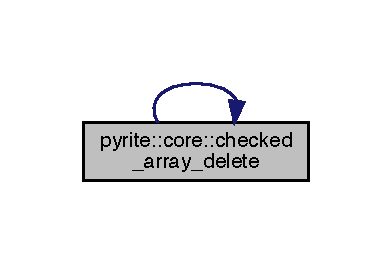
\includegraphics[width=188pt]{d5/d3a/checked__delete_8hpp_a47e9f6f9578e0518074ca6da633d7ea8_cgraph}
\end{center}
\end{figure}
Here is the caller graph for this function\+:
\nopagebreak
\begin{figure}[H]
\begin{center}
\leavevmode
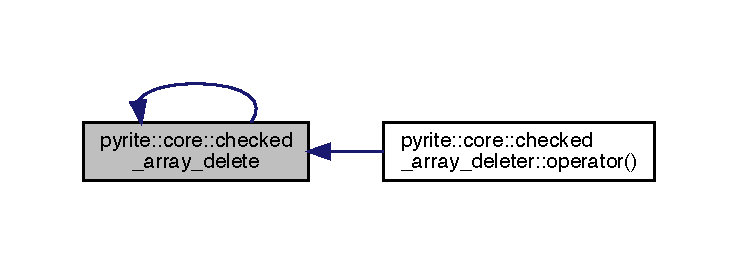
\includegraphics[width=350pt]{d5/d3a/checked__delete_8hpp_a47e9f6f9578e0518074ca6da633d7ea8_icgraph}
\end{center}
\end{figure}
\mbox{\Hypertarget{checked__delete_8hpp_file_a27af49b4f86442c78de48cda0818eb72}\label{checked__delete_8hpp_file_a27af49b4f86442c78de48cda0818eb72}} 
\index{checked\+\_\+delete.\+hpp@{checked\+\_\+delete.\+hpp}!checked\+\_\+delete@{checked\+\_\+delete}}
\index{checked\+\_\+delete@{checked\+\_\+delete}!checked\+\_\+delete.\+hpp@{checked\+\_\+delete.\+hpp}}
\subsubsection{\texorpdfstring{checked\+\_\+delete()}{checked\_delete()}}
{\footnotesize\ttfamily template$<$typename T $>$ \\
void pyrite\+::core\+::checked\+\_\+delete (\begin{DoxyParamCaption}\item[{T $\ast$\&}]{ptr }\end{DoxyParamCaption})}

After deleting the pointer, assing nullptr. 
\begin{DoxyTemplParams}{Template Parameters}
{\em T} & T must be a complete type. \\
\hline
\end{DoxyTemplParams}

\begin{DoxyParams}{Parameters}
{\em ptr} & pointer. \\
\hline
\end{DoxyParams}
Here is the call graph for this function\+:
\nopagebreak
\begin{figure}[H]
\begin{center}
\leavevmode
\includegraphics[width=188pt]{d5/d3a/checked__delete_8hpp_a27af49b4f86442c78de48cda0818eb72_cgraph}
\end{center}
\end{figure}
Here is the caller graph for this function\+:
\nopagebreak
\begin{figure}[H]
\begin{center}
\leavevmode
\includegraphics[width=333pt]{d5/d3a/checked__delete_8hpp_a27af49b4f86442c78de48cda0818eb72_icgraph}
\end{center}
\end{figure}

\hypertarget{detail_2type_8hpp}{}\section{/\+Users/masato.tanaka/\+Development/cpp/pyrite/pyrite/core/detail/type.hpp File Reference}
\label{detail_2type_8hpp}\index{/\+Users/masato.\+tanaka/\+Development/cpp/pyrite/pyrite/core/detail/type.\+hpp@{/\+Users/masato.\+tanaka/\+Development/cpp/pyrite/pyrite/core/detail/type.\+hpp}}
{\ttfamily \#include $<$type\+\_\+traits$>$}\newline
{\ttfamily \#include $<$pyrite/core/mpl/type\+\_\+list.\+hpp$>$}\newline
{\ttfamily \#include $<$pyrite/core/mpl/type\+\_\+list/find\+\_\+if.\+hpp$>$}\newline
Include dependency graph for type.\+hpp\+:
\nopagebreak
\begin{figure}[H]
\begin{center}
\leavevmode
\includegraphics[width=350pt]{db/dd3/detail_2type_8hpp__incl}
\end{center}
\end{figure}
This graph shows which files directly or indirectly include this file\+:
\nopagebreak
\begin{figure}[H]
\begin{center}
\leavevmode
\includegraphics[width=350pt]{d6/d13/detail_2type_8hpp__dep__incl}
\end{center}
\end{figure}
\subsection*{Typedefs}
\begin{DoxyCompactItemize}
\item 
\mbox{\Hypertarget{detail_2type_8hpp_a7fd464f79f9188c8fe8ead38a1718b61}\label{detail_2type_8hpp_a7fd464f79f9188c8fe8ead38a1718b61}} 
using {\bfseries pyrite\+::core\+::i8} = find\+\_\+from\+\_\+size\+\_\+t$<$ signed\+\_\+list, 1u $>$
\item 
\mbox{\Hypertarget{detail_2type_8hpp_ac48271d799022c1057c5ec78a9703a07}\label{detail_2type_8hpp_ac48271d799022c1057c5ec78a9703a07}} 
using {\bfseries pyrite\+::core\+::i16} = find\+\_\+from\+\_\+size\+\_\+t$<$ signed\+\_\+list, 2u $>$
\item 
\mbox{\Hypertarget{detail_2type_8hpp_ae65a35cd17f4f6224c707d3b8939b7b0}\label{detail_2type_8hpp_ae65a35cd17f4f6224c707d3b8939b7b0}} 
using {\bfseries pyrite\+::core\+::i32} = find\+\_\+from\+\_\+size\+\_\+t$<$ signed\+\_\+list, 4u $>$
\item 
\mbox{\Hypertarget{detail_2type_8hpp_aa74553a427e44eaa232057b02b67c8b3}\label{detail_2type_8hpp_aa74553a427e44eaa232057b02b67c8b3}} 
using {\bfseries pyrite\+::core\+::i64} = find\+\_\+from\+\_\+size\+\_\+t$<$ signed\+\_\+list, 8u $>$
\item 
\mbox{\Hypertarget{detail_2type_8hpp_a63dcab02b1104867fd219f2dc2a46a6c}\label{detail_2type_8hpp_a63dcab02b1104867fd219f2dc2a46a6c}} 
using {\bfseries pyrite\+::core\+::u8} = find\+\_\+from\+\_\+size\+\_\+t$<$ unsigned\+\_\+list, 1u $>$
\item 
\mbox{\Hypertarget{detail_2type_8hpp_a154bced535ef32062ff6969effd31c9a}\label{detail_2type_8hpp_a154bced535ef32062ff6969effd31c9a}} 
using {\bfseries pyrite\+::core\+::u16} = find\+\_\+from\+\_\+size\+\_\+t$<$ unsigned\+\_\+list, 2u $>$
\item 
\mbox{\Hypertarget{detail_2type_8hpp_a672cb423ff58f39502f116d00cab74dd}\label{detail_2type_8hpp_a672cb423ff58f39502f116d00cab74dd}} 
using {\bfseries pyrite\+::core\+::u32} = find\+\_\+from\+\_\+size\+\_\+t$<$ unsigned\+\_\+list, 4u $>$
\item 
\mbox{\Hypertarget{detail_2type_8hpp_a076b0568a7156266938bfacb53d17f7e}\label{detail_2type_8hpp_a076b0568a7156266938bfacb53d17f7e}} 
using {\bfseries pyrite\+::core\+::u64} = find\+\_\+from\+\_\+size\+\_\+t$<$ unsigned\+\_\+list, 8u $>$
\item 
\mbox{\Hypertarget{detail_2type_8hpp_aa5cf207ff3d2d26ff45e63a78c0d7cda}\label{detail_2type_8hpp_aa5cf207ff3d2d26ff45e63a78c0d7cda}} 
using {\bfseries pyrite\+::core\+::f32} = find\+\_\+from\+\_\+size\+\_\+t$<$ floating\+\_\+point\+\_\+list, 4u $>$
\item 
\mbox{\Hypertarget{detail_2type_8hpp_ac0bd1ecb2c19d585c3257837588acc31}\label{detail_2type_8hpp_ac0bd1ecb2c19d585c3257837588acc31}} 
using {\bfseries pyrite\+::core\+::f64} = find\+\_\+from\+\_\+size\+\_\+t$<$ floating\+\_\+point\+\_\+list, 8u $>$
\item 
\mbox{\Hypertarget{detail_2type_8hpp_ac6463df11829a4d4891026f927acacdb}\label{detail_2type_8hpp_ac6463df11829a4d4891026f927acacdb}} 
using {\bfseries pyrite\+::core\+::isize} = find\+\_\+from\+\_\+size\+\_\+t$<$ signed\+\_\+list, max(sizeof(std\+::size\+\_\+t), std\+::size\+\_\+t\{8u\})$>$
\item 
\mbox{\Hypertarget{detail_2type_8hpp_a145f18ea1381c083f26a4397d8a82eb3}\label{detail_2type_8hpp_a145f18ea1381c083f26a4397d8a82eb3}} 
using {\bfseries pyrite\+::core\+::usize} = find\+\_\+from\+\_\+size\+\_\+t$<$ unsigned\+\_\+list, max(sizeof(std\+::size\+\_\+t), std\+::size\+\_\+t\{8u\})$>$
\item 
\mbox{\Hypertarget{detail_2type_8hpp_ad78d654d9fe1e5861e7a01a33eba3507}\label{detail_2type_8hpp_ad78d654d9fe1e5861e7a01a33eba3507}} 
using {\bfseries pyrite\+::core\+::iptr} = find\+\_\+from\+\_\+size\+\_\+t$<$ signed\+\_\+list, sizeof(int $\ast$)$>$
\item 
\mbox{\Hypertarget{detail_2type_8hpp_a290fc2b170cf83d229c9f5f4d59417bb}\label{detail_2type_8hpp_a290fc2b170cf83d229c9f5f4d59417bb}} 
using {\bfseries pyrite\+::core\+::uptr} = find\+\_\+from\+\_\+size\+\_\+t$<$ unsigned\+\_\+list, sizeof(int $\ast$)$>$
\item 
\mbox{\Hypertarget{detail_2type_8hpp_a516618865550504db165a0f2d5090d22}\label{detail_2type_8hpp_a516618865550504db165a0f2d5090d22}} 
using {\bfseries pyrite\+::core\+::ptrdiff} = decltype(std\+::declval$<$ int $\ast$ $>$() -\/ std\+::declval$<$ int $\ast$ $>$())
\end{DoxyCompactItemize}


\subsection{Detailed Description}
\begin{DoxyAuthor}{Author}
block 
\end{DoxyAuthor}
\begin{DoxyCopyright}{Copyright}
(c) 2018 block. 
\end{DoxyCopyright}

\hypertarget{type_8hpp}{}\section{/\+Users/masato.tanaka/\+Development/cpp/pyrite/pyrite/core/type.hpp File Reference}
\label{type_8hpp}\index{/\+Users/masato.\+tanaka/\+Development/cpp/pyrite/pyrite/core/type.\+hpp@{/\+Users/masato.\+tanaka/\+Development/cpp/pyrite/pyrite/core/type.\+hpp}}
{\ttfamily \#include $<$pyrite/core/detail/type.\+hpp$>$}\newline
Include dependency graph for type.\+hpp\+:
\nopagebreak
\begin{figure}[H]
\begin{center}
\leavevmode
\includegraphics[width=350pt]{d2/deb/type_8hpp__incl}
\end{center}
\end{figure}
This graph shows which files directly or indirectly include this file\+:
\nopagebreak
\begin{figure}[H]
\begin{center}
\leavevmode
\includegraphics[width=350pt]{d9/d43/type_8hpp__dep__incl}
\end{center}
\end{figure}
\subsection*{Typedefs}
\begin{DoxyCompactItemize}
\item 
\mbox{\Hypertarget{type_8hpp_a6c192ecd67d26cb37aa7b9f9d919995e}\label{type_8hpp_a6c192ecd67d26cb37aa7b9f9d919995e}} 
using \mbox{\hyperlink{type_8hpp_a6c192ecd67d26cb37aa7b9f9d919995e}{pyrite\+::i8}} = core\+::i8
\begin{DoxyCompactList}\small\item\em 8 bit signed integer type. \end{DoxyCompactList}\item 
\mbox{\Hypertarget{type_8hpp_afb472e1d3eeee625f2a101ee18b4d8f6}\label{type_8hpp_afb472e1d3eeee625f2a101ee18b4d8f6}} 
using \mbox{\hyperlink{type_8hpp_afb472e1d3eeee625f2a101ee18b4d8f6}{pyrite\+::i16}} = core\+::i16
\begin{DoxyCompactList}\small\item\em 16 bit signed integer type. \end{DoxyCompactList}\item 
\mbox{\Hypertarget{type_8hpp_aba0d848c44be3eae1f652255da3ffbbd}\label{type_8hpp_aba0d848c44be3eae1f652255da3ffbbd}} 
using \mbox{\hyperlink{type_8hpp_aba0d848c44be3eae1f652255da3ffbbd}{pyrite\+::i32}} = core\+::i32
\begin{DoxyCompactList}\small\item\em 32 bit signed integer type. \end{DoxyCompactList}\item 
\mbox{\Hypertarget{type_8hpp_a065f829bff902708107ee01e67bf81cb}\label{type_8hpp_a065f829bff902708107ee01e67bf81cb}} 
using \mbox{\hyperlink{type_8hpp_a065f829bff902708107ee01e67bf81cb}{pyrite\+::i64}} = core\+::i64
\begin{DoxyCompactList}\small\item\em 64 bit signed integer type. \end{DoxyCompactList}\item 
\mbox{\Hypertarget{type_8hpp_ab3c6f42f8cedf53800f98e10e46a6d00}\label{type_8hpp_ab3c6f42f8cedf53800f98e10e46a6d00}} 
using \mbox{\hyperlink{type_8hpp_ab3c6f42f8cedf53800f98e10e46a6d00}{pyrite\+::u8}} = core\+::u8
\begin{DoxyCompactList}\small\item\em 8 bit unsigned integer type. \end{DoxyCompactList}\item 
\mbox{\Hypertarget{type_8hpp_afd20dadb4dfb0619217621893b3732ae}\label{type_8hpp_afd20dadb4dfb0619217621893b3732ae}} 
using \mbox{\hyperlink{type_8hpp_afd20dadb4dfb0619217621893b3732ae}{pyrite\+::u16}} = core\+::u16
\begin{DoxyCompactList}\small\item\em 16 bit unsigned integer type. \end{DoxyCompactList}\item 
\mbox{\Hypertarget{type_8hpp_a560d2b714b6a16842b5ad7900547ab50}\label{type_8hpp_a560d2b714b6a16842b5ad7900547ab50}} 
using \mbox{\hyperlink{type_8hpp_a560d2b714b6a16842b5ad7900547ab50}{pyrite\+::u32}} = core\+::u32
\begin{DoxyCompactList}\small\item\em 32 bit unsigned integer type. \end{DoxyCompactList}\item 
\mbox{\Hypertarget{type_8hpp_a89cb75b6e56f357c2964bbd5520be899}\label{type_8hpp_a89cb75b6e56f357c2964bbd5520be899}} 
using \mbox{\hyperlink{type_8hpp_a89cb75b6e56f357c2964bbd5520be899}{pyrite\+::u64}} = core\+::u64
\begin{DoxyCompactList}\small\item\em 64 bit unsigned integer type. \end{DoxyCompactList}\item 
\mbox{\Hypertarget{type_8hpp_af788503491e8b49a2cbb94a5b7caa807}\label{type_8hpp_af788503491e8b49a2cbb94a5b7caa807}} 
using \mbox{\hyperlink{type_8hpp_af788503491e8b49a2cbb94a5b7caa807}{pyrite\+::f32}} = core\+::f32
\begin{DoxyCompactList}\small\item\em 32 bit floating point type. \end{DoxyCompactList}\item 
\mbox{\Hypertarget{type_8hpp_a09fd802f4dadecc46f8df0a27ae03209}\label{type_8hpp_a09fd802f4dadecc46f8df0a27ae03209}} 
using \mbox{\hyperlink{type_8hpp_a09fd802f4dadecc46f8df0a27ae03209}{pyrite\+::f64}} = core\+::f64
\begin{DoxyCompactList}\small\item\em 64 bit floating point type. \end{DoxyCompactList}\item 
\mbox{\Hypertarget{type_8hpp_a2decee739e771a9008f4c0b04eff2704}\label{type_8hpp_a2decee739e771a9008f4c0b04eff2704}} 
using \mbox{\hyperlink{type_8hpp_a2decee739e771a9008f4c0b04eff2704}{pyrite\+::isize}} = core\+::isize
\begin{DoxyCompactList}\small\item\em Signed intger type large enough to represent size. \end{DoxyCompactList}\item 
\mbox{\Hypertarget{type_8hpp_a3984e6dc0a53b867e054e8447f2f2be1}\label{type_8hpp_a3984e6dc0a53b867e054e8447f2f2be1}} 
using \mbox{\hyperlink{type_8hpp_a3984e6dc0a53b867e054e8447f2f2be1}{pyrite\+::usize}} = core\+::usize
\begin{DoxyCompactList}\small\item\em Unsigned intger type large enough to represent size. \end{DoxyCompactList}\item 
\mbox{\Hypertarget{type_8hpp_a975daf4d2f09d9c3683ad9c3e138a0a0}\label{type_8hpp_a975daf4d2f09d9c3683ad9c3e138a0a0}} 
using {\bfseries pyrite\+::byte} = u8
\item 
\mbox{\Hypertarget{type_8hpp_afee1b29cc7b0024bcd659f6d96a5c3a2}\label{type_8hpp_afee1b29cc7b0024bcd659f6d96a5c3a2}} 
using {\bfseries pyrite\+::iptr} = core\+::iptr
\item 
\mbox{\Hypertarget{type_8hpp_a34d687a5834b74dd531dacacaa83b5d3}\label{type_8hpp_a34d687a5834b74dd531dacacaa83b5d3}} 
using {\bfseries pyrite\+::uptr} = core\+::uptr
\item 
\mbox{\Hypertarget{type_8hpp_aaf932bb70bbf32a656b0f19db4209934}\label{type_8hpp_aaf932bb70bbf32a656b0f19db4209934}} 
using {\bfseries pyrite\+::ptrdiff} = core\+::ptrdiff
\end{DoxyCompactItemize}


\subsection{Detailed Description}
\begin{DoxyAuthor}{Author}
block 
\end{DoxyAuthor}
\begin{DoxyCopyright}{Copyright}
(c) 2018 block. 
\end{DoxyCopyright}

\hypertarget{endian_8hpp}{}\section{/\+Users/masato.tanaka/\+Development/cpp/pyrite/pyrite/core/endian.hpp File Reference}
\label{endian_8hpp}\index{/\+Users/masato.\+tanaka/\+Development/cpp/pyrite/pyrite/core/endian.\+hpp@{/\+Users/masato.\+tanaka/\+Development/cpp/pyrite/pyrite/core/endian.\+hpp}}
{\ttfamily \#include $<$pyrite/core/type.\+hpp$>$}\newline
Include dependency graph for endian.\+hpp\+:
\nopagebreak
\begin{figure}[H]
\begin{center}
\leavevmode
\includegraphics[width=350pt]{d0/dbd/endian_8hpp__incl}
\end{center}
\end{figure}
This graph shows which files directly or indirectly include this file\+:
\nopagebreak
\begin{figure}[H]
\begin{center}
\leavevmode
\includegraphics[width=204pt]{db/dd6/endian_8hpp__dep__incl}
\end{center}
\end{figure}
\subsection*{Enumerations}
\begin{DoxyCompactItemize}
\item 
enum \mbox{\hyperlink{endian_8hpp_a720a76d266d91e0e4114430ff550ff2e}{pyrite\+::core\+::endian}} \+: i8 \{ {\bfseries pyrite\+::core\+::endian\+::big}, 
{\bfseries pyrite\+::core\+::endian\+::little}, 
{\bfseries pyrite\+::core\+::endian\+::native} =
 \}
\end{DoxyCompactItemize}


\subsection{Detailed Description}
\begin{DoxyAuthor}{Author}
block 
\end{DoxyAuthor}
\begin{DoxyCopyright}{Copyright}
(c) 2018 block. 
\end{DoxyCopyright}


\subsection{Enumeration Type Documentation}
\mbox{\Hypertarget{endian_8hpp_file_a720a76d266d91e0e4114430ff550ff2e}\label{endian_8hpp_file_a720a76d266d91e0e4114430ff550ff2e}} 
\index{endian.\+hpp@{endian.\+hpp}!endian@{endian}}
\index{endian@{endian}!endian.\+hpp@{endian.\+hpp}}
\subsubsection{\texorpdfstring{endian}{endian}}
{\footnotesize\ttfamily enum \mbox{\hyperlink{endian_8hpp_a720a76d266d91e0e4114430ff550ff2e}{pyrite\+::core\+::endian}} \+: i8\hspace{0.3cm}{\ttfamily [strong]}}

An enumerated type representing the order of bytes (endian). 
\hypertarget{core_2is__complete__type_8hpp}{}\section{/\+Users/masato.tanaka/\+Development/cpp/pyrite/pyrite/core/is\+\_\+complete\+\_\+type.hpp File Reference}
\label{core_2is__complete__type_8hpp}\index{/\+Users/masato.\+tanaka/\+Development/cpp/pyrite/pyrite/core/is\+\_\+complete\+\_\+type.\+hpp@{/\+Users/masato.\+tanaka/\+Development/cpp/pyrite/pyrite/core/is\+\_\+complete\+\_\+type.\+hpp}}
{\ttfamily \#include $<$type\+\_\+traits$>$}\newline
Include dependency graph for is\+\_\+complete\+\_\+type.\+hpp\+:
\nopagebreak
\begin{figure}[H]
\begin{center}
\leavevmode
\includegraphics[width=204pt]{d3/d08/core_2is__complete__type_8hpp__incl}
\end{center}
\end{figure}
This graph shows which files directly or indirectly include this file\+:
\nopagebreak
\begin{figure}[H]
\begin{center}
\leavevmode
\includegraphics[width=350pt]{dc/d08/core_2is__complete__type_8hpp__dep__incl}
\end{center}
\end{figure}
\subsection*{Classes}
\begin{DoxyCompactItemize}
\item 
class \mbox{\hyperlink{classpyrite_1_1core_1_1is__complete__type}{pyrite\+::core\+::is\+\_\+complete\+\_\+type$<$ T, typename $>$}}
\item 
class \mbox{\hyperlink{classpyrite_1_1core_1_1is__complete__type_3_01_t_00_01std_1_1void__t_3_01decltype_07sizeof_07_t_08_08_4_01_4}{pyrite\+::core\+::is\+\_\+complete\+\_\+type$<$ T, std\+::void\+\_\+t$<$ decltype(sizeof(\+T))$>$ $>$}}
\end{DoxyCompactItemize}
\subsection*{Variables}
\begin{DoxyCompactItemize}
\item 
{\footnotesize template$<$typename T $>$ }\\constexpr bool \mbox{\hyperlink{core_2is__complete__type_8hpp_a1a6a901231504b05c90c769a03aa16f4}{pyrite\+::core\+::is\+\_\+complete\+\_\+type\+\_\+v}} = is\+\_\+complete\+\_\+type$<$T$>$\+::value
\end{DoxyCompactItemize}


\subsection{Detailed Description}
\begin{DoxyAuthor}{Author}
block 
\end{DoxyAuthor}
\begin{DoxyCopyright}{Copyright}
(c) 2018 block. 
\end{DoxyCopyright}


\subsection{Variable Documentation}
\mbox{\Hypertarget{core_2is__complete__type_8hpp_file_a1a6a901231504b05c90c769a03aa16f4}\label{core_2is__complete__type_8hpp_file_a1a6a901231504b05c90c769a03aa16f4}} 
\index{core/is\+\_\+complete\+\_\+type.\+hpp@{core/is\+\_\+complete\+\_\+type.\+hpp}!is\+\_\+complete\+\_\+type\+\_\+v@{is\+\_\+complete\+\_\+type\+\_\+v}}
\index{is\+\_\+complete\+\_\+type\+\_\+v@{is\+\_\+complete\+\_\+type\+\_\+v}!core/is\+\_\+complete\+\_\+type.\+hpp@{core/is\+\_\+complete\+\_\+type.\+hpp}}
\subsubsection{\texorpdfstring{is\+\_\+complete\+\_\+type\+\_\+v}{is\_complete\_type\_v}}
{\footnotesize\ttfamily template$<$typename T $>$ \\
constexpr bool pyrite\+::core\+::is\+\_\+complete\+\_\+type\+\_\+v = is\+\_\+complete\+\_\+type$<$T$>$\+::value}

Variable template version of is\+\_\+complete\+\_\+type. 
\hypertarget{type__traits_2is__complete__type_8hpp}{}\section{/\+Users/masato.tanaka/\+Development/cpp/pyrite/pyrite/type\+\_\+traits/is\+\_\+complete\+\_\+type.hpp File Reference}
\label{type__traits_2is__complete__type_8hpp}\index{/\+Users/masato.\+tanaka/\+Development/cpp/pyrite/pyrite/type\+\_\+traits/is\+\_\+complete\+\_\+type.\+hpp@{/\+Users/masato.\+tanaka/\+Development/cpp/pyrite/pyrite/type\+\_\+traits/is\+\_\+complete\+\_\+type.\+hpp}}
{\ttfamily \#include $<$pyrite/core/is\+\_\+complete\+\_\+type.\+hpp$>$}\newline
Include dependency graph for is\+\_\+complete\+\_\+type.\+hpp\+:
\nopagebreak
\begin{figure}[H]
\begin{center}
\leavevmode
\includegraphics[width=204pt]{d7/d26/type__traits_2is__complete__type_8hpp__incl}
\end{center}
\end{figure}


\subsection{Detailed Description}
\begin{DoxyAuthor}{Author}
block 
\end{DoxyAuthor}
\begin{DoxyCopyright}{Copyright}
(c) 2018 block. 
\end{DoxyCopyright}

\hypertarget{core_2mpl_2type__list_2filter_8hpp}{}\section{/\+Users/masato.tanaka/\+Development/cpp/pyrite/pyrite/core/mpl/type\+\_\+list/filter.hpp File Reference}
\label{core_2mpl_2type__list_2filter_8hpp}\index{/\+Users/masato.\+tanaka/\+Development/cpp/pyrite/pyrite/core/mpl/type\+\_\+list/filter.\+hpp@{/\+Users/masato.\+tanaka/\+Development/cpp/pyrite/pyrite/core/mpl/type\+\_\+list/filter.\+hpp}}
{\ttfamily \#include $<$type\+\_\+traits$>$}\newline
{\ttfamily \#include $<$pyrite/core/mpl/type\+\_\+list/is\+\_\+type\+\_\+list.\+hpp$>$}\newline
{\ttfamily \#include $<$pyrite/core/mpl/type\+\_\+list/operators.\+hpp$>$}\newline
{\ttfamily \#include $<$pyrite/core/mpl/type\+\_\+list/type\+\_\+list.\+hpp$>$}\newline
{\ttfamily \#include $<$pyrite/core/mpl/type\+\_\+optional.\+hpp$>$}\newline
Include dependency graph for filter.\+hpp\+:
\nopagebreak
\begin{figure}[H]
\begin{center}
\leavevmode
\includegraphics[width=350pt]{d8/dda/core_2mpl_2type__list_2filter_8hpp__incl}
\end{center}
\end{figure}
This graph shows which files directly or indirectly include this file\+:
\nopagebreak
\begin{figure}[H]
\begin{center}
\leavevmode
\includegraphics[width=350pt]{d2/d9e/core_2mpl_2type__list_2filter_8hpp__dep__incl}
\end{center}
\end{figure}
\subsection*{Classes}
\begin{DoxyCompactItemize}
\item 
struct \mbox{\hyperlink{structpyrite_1_1core_1_1mpl_1_1filter}{pyrite\+::core\+::mpl\+::filter$<$ List, F $>$}}
\item 
struct \mbox{\hyperlink{structpyrite_1_1core_1_1mpl_1_1filter_3_01type__list_3_01_args_8_8_8_01_4_00_01_f_01_4}{pyrite\+::core\+::mpl\+::filter$<$ type\+\_\+list$<$ Args... $>$, F $>$}}
\end{DoxyCompactItemize}
\subsection*{Typedefs}
\begin{DoxyCompactItemize}
\item 
\mbox{\Hypertarget{core_2mpl_2type__list_2filter_8hpp_ad765da5cbb1d966a35e138abddfbe73d}\label{core_2mpl_2type__list_2filter_8hpp_ad765da5cbb1d966a35e138abddfbe73d}} 
{\footnotesize template$<$typename List , template$<$ typename $>$ typename F$>$ }\\using {\bfseries pyrite\+::core\+::mpl\+::filter\+\_\+t} = typename filter$<$ List, F $>$\+::type
\end{DoxyCompactItemize}


\subsection{Detailed Description}
\begin{DoxyAuthor}{Author}
block 
\end{DoxyAuthor}
\begin{DoxyCopyright}{Copyright}
(c) 2018 block. 
\end{DoxyCopyright}

\hypertarget{mpl_2type__list_2filter_8hpp}{}\section{/\+Users/masato.tanaka/\+Development/cpp/pyrite/pyrite/mpl/type\+\_\+list/filter.hpp File Reference}
\label{mpl_2type__list_2filter_8hpp}\index{/\+Users/masato.\+tanaka/\+Development/cpp/pyrite/pyrite/mpl/type\+\_\+list/filter.\+hpp@{/\+Users/masato.\+tanaka/\+Development/cpp/pyrite/pyrite/mpl/type\+\_\+list/filter.\+hpp}}
{\ttfamily \#include $<$pyrite/core/mpl/type\+\_\+list/filter.\+hpp$>$}\newline
Include dependency graph for filter.\+hpp\+:
\nopagebreak
\begin{figure}[H]
\begin{center}
\leavevmode
\includegraphics[width=350pt]{da/d26/mpl_2type__list_2filter_8hpp__incl}
\end{center}
\end{figure}
This graph shows which files directly or indirectly include this file\+:
\nopagebreak
\begin{figure}[H]
\begin{center}
\leavevmode
\includegraphics[width=222pt]{de/de1/mpl_2type__list_2filter_8hpp__dep__incl}
\end{center}
\end{figure}


\subsection{Detailed Description}
\begin{DoxyAuthor}{Author}
block 
\end{DoxyAuthor}
\begin{DoxyCopyright}{Copyright}
(c) 2018 block. 
\end{DoxyCopyright}

\hypertarget{core_2mpl_2type__list_2find__if_8hpp}{}\section{/\+Users/masato.tanaka/\+Development/cpp/pyrite/pyrite/core/mpl/type\+\_\+list/find\+\_\+if.hpp File Reference}
\label{core_2mpl_2type__list_2find__if_8hpp}\index{/\+Users/masato.\+tanaka/\+Development/cpp/pyrite/pyrite/core/mpl/type\+\_\+list/find\+\_\+if.\+hpp@{/\+Users/masato.\+tanaka/\+Development/cpp/pyrite/pyrite/core/mpl/type\+\_\+list/find\+\_\+if.\+hpp}}
{\ttfamily \#include $<$pyrite/core/mpl/type\+\_\+list/filter.\+hpp$>$}\newline
{\ttfamily \#include $<$pyrite/core/mpl/type\+\_\+list/head.\+hpp$>$}\newline
{\ttfamily \#include $<$pyrite/core/mpl/type\+\_\+list/is\+\_\+type\+\_\+list.\+hpp$>$}\newline
{\ttfamily \#include $<$pyrite/core/mpl/type\+\_\+optional.\+hpp$>$}\newline
Include dependency graph for find\+\_\+if.\+hpp\+:
\nopagebreak
\begin{figure}[H]
\begin{center}
\leavevmode
\includegraphics[width=350pt]{db/d21/core_2mpl_2type__list_2find__if_8hpp__incl}
\end{center}
\end{figure}
This graph shows which files directly or indirectly include this file\+:
\nopagebreak
\begin{figure}[H]
\begin{center}
\leavevmode
\includegraphics[width=350pt]{d5/d72/core_2mpl_2type__list_2find__if_8hpp__dep__incl}
\end{center}
\end{figure}
\subsection*{Classes}
\begin{DoxyCompactItemize}
\item 
struct \mbox{\hyperlink{structpyrite_1_1core_1_1mpl_1_1find__if}{pyrite\+::core\+::mpl\+::find\+\_\+if$<$ List, F $>$}}
\end{DoxyCompactItemize}
\subsection*{Typedefs}
\begin{DoxyCompactItemize}
\item 
\mbox{\Hypertarget{core_2mpl_2type__list_2find__if_8hpp_aef36bf85ded1884537104d6be73b903c}\label{core_2mpl_2type__list_2find__if_8hpp_aef36bf85ded1884537104d6be73b903c}} 
{\footnotesize template$<$typename List , template$<$ typename $>$ typename F$>$ }\\using {\bfseries pyrite\+::core\+::mpl\+::find\+\_\+if\+\_\+t} = typename find\+\_\+if$<$ List, F $>$\+::type
\end{DoxyCompactItemize}


\subsection{Detailed Description}
\begin{DoxyAuthor}{Author}
block 
\end{DoxyAuthor}
\begin{DoxyCopyright}{Copyright}
(c) 2018 block. 
\end{DoxyCopyright}

\hypertarget{mpl_2type__list_2find__if_8hpp}{}\section{/\+Users/masato.tanaka/\+Development/cpp/pyrite/pyrite/mpl/type\+\_\+list/find\+\_\+if.hpp File Reference}
\label{mpl_2type__list_2find__if_8hpp}\index{/\+Users/masato.\+tanaka/\+Development/cpp/pyrite/pyrite/mpl/type\+\_\+list/find\+\_\+if.\+hpp@{/\+Users/masato.\+tanaka/\+Development/cpp/pyrite/pyrite/mpl/type\+\_\+list/find\+\_\+if.\+hpp}}
{\ttfamily \#include $<$pyrite/core/mpl/type\+\_\+list/find\+\_\+if.\+hpp$>$}\newline
Include dependency graph for find\+\_\+if.\+hpp\+:
\nopagebreak
\begin{figure}[H]
\begin{center}
\leavevmode
\includegraphics[width=350pt]{d9/de5/mpl_2type__list_2find__if_8hpp__incl}
\end{center}
\end{figure}
This graph shows which files directly or indirectly include this file\+:
\nopagebreak
\begin{figure}[H]
\begin{center}
\leavevmode
\includegraphics[width=332pt]{db/d32/mpl_2type__list_2find__if_8hpp__dep__incl}
\end{center}
\end{figure}


\subsection{Detailed Description}
\begin{DoxyAuthor}{Author}
block 
\end{DoxyAuthor}
\begin{DoxyCopyright}{Copyright}
(c) 2018 block. 
\end{DoxyCopyright}

\hypertarget{core_2mpl_2type__list_2head_8hpp}{}\section{/\+Users/masato.tanaka/\+Development/cpp/pyrite/pyrite/core/mpl/type\+\_\+list/head.hpp File Reference}
\label{core_2mpl_2type__list_2head_8hpp}\index{/\+Users/masato.\+tanaka/\+Development/cpp/pyrite/pyrite/core/mpl/type\+\_\+list/head.\+hpp@{/\+Users/masato.\+tanaka/\+Development/cpp/pyrite/pyrite/core/mpl/type\+\_\+list/head.\+hpp}}
{\ttfamily \#include $<$pyrite/core/mpl/type\+\_\+list/is\+\_\+type\+\_\+list.\+hpp$>$}\newline
{\ttfamily \#include $<$pyrite/core/mpl/type\+\_\+list/type\+\_\+list.\+hpp$>$}\newline
{\ttfamily \#include $<$pyrite/core/mpl/type\+\_\+optional.\+hpp$>$}\newline
Include dependency graph for head.\+hpp\+:
\nopagebreak
\begin{figure}[H]
\begin{center}
\leavevmode
\includegraphics[width=345pt]{d0/dd7/core_2mpl_2type__list_2head_8hpp__incl}
\end{center}
\end{figure}
This graph shows which files directly or indirectly include this file\+:
\nopagebreak
\begin{figure}[H]
\begin{center}
\leavevmode
\includegraphics[width=350pt]{df/d50/core_2mpl_2type__list_2head_8hpp__dep__incl}
\end{center}
\end{figure}
\subsection*{Classes}
\begin{DoxyCompactItemize}
\item 
struct \mbox{\hyperlink{structpyrite_1_1core_1_1mpl_1_1head}{pyrite\+::core\+::mpl\+::head$<$ T $>$}}
\item 
struct \mbox{\hyperlink{structpyrite_1_1core_1_1mpl_1_1head_3_01type__list_3_01_head_00_01_tail_8_8_8_01_4_01_4}{pyrite\+::core\+::mpl\+::head$<$ type\+\_\+list$<$ Head, Tail... $>$ $>$}}
\end{DoxyCompactItemize}
\subsection*{Typedefs}
\begin{DoxyCompactItemize}
\item 
\mbox{\Hypertarget{core_2mpl_2type__list_2head_8hpp_aa6c1702cdad0d5b350ca8cc4eeed3869}\label{core_2mpl_2type__list_2head_8hpp_aa6c1702cdad0d5b350ca8cc4eeed3869}} 
{\footnotesize template$<$typename List $>$ }\\using {\bfseries pyrite\+::core\+::mpl\+::head\+\_\+t} = typename head$<$ List $>$\+::type
\end{DoxyCompactItemize}


\subsection{Detailed Description}
\begin{DoxyAuthor}{Author}
block 
\end{DoxyAuthor}
\begin{DoxyCopyright}{Copyright}
(c) 2018 block. 
\end{DoxyCopyright}

\hypertarget{mpl_2type__list_2head_8hpp}{}\section{/\+Users/masato.tanaka/\+Development/cpp/pyrite/pyrite/mpl/type\+\_\+list/head.hpp File Reference}
\label{mpl_2type__list_2head_8hpp}\index{/\+Users/masato.\+tanaka/\+Development/cpp/pyrite/pyrite/mpl/type\+\_\+list/head.\+hpp@{/\+Users/masato.\+tanaka/\+Development/cpp/pyrite/pyrite/mpl/type\+\_\+list/head.\+hpp}}
{\ttfamily \#include $<$pyrite/core/mpl/type\+\_\+list/head.\+hpp$>$}\newline
Include dependency graph for head.\+hpp\+:
\nopagebreak
\begin{figure}[H]
\begin{center}
\leavevmode
\includegraphics[width=345pt]{d6/da6/mpl_2type__list_2head_8hpp__incl}
\end{center}
\end{figure}
This graph shows which files directly or indirectly include this file\+:
\nopagebreak
\begin{figure}[H]
\begin{center}
\leavevmode
\includegraphics[width=226pt]{d7/dd9/mpl_2type__list_2head_8hpp__dep__incl}
\end{center}
\end{figure}


\subsection{Detailed Description}
\begin{DoxyAuthor}{Author}
block 
\end{DoxyAuthor}
\begin{DoxyCopyright}{Copyright}
(c) 2018 block. 
\end{DoxyCopyright}

\hypertarget{core_2mpl_2type__list_2is__type__list_8hpp}{}\section{/\+Users/masato.tanaka/\+Development/cpp/pyrite/pyrite/core/mpl/type\+\_\+list/is\+\_\+type\+\_\+list.hpp File Reference}
\label{core_2mpl_2type__list_2is__type__list_8hpp}\index{/\+Users/masato.\+tanaka/\+Development/cpp/pyrite/pyrite/core/mpl/type\+\_\+list/is\+\_\+type\+\_\+list.\+hpp@{/\+Users/masato.\+tanaka/\+Development/cpp/pyrite/pyrite/core/mpl/type\+\_\+list/is\+\_\+type\+\_\+list.\+hpp}}
{\ttfamily \#include $<$type\+\_\+traits$>$}\newline
{\ttfamily \#include $<$pyrite/core/mpl/type\+\_\+list/type\+\_\+list.\+hpp$>$}\newline
Include dependency graph for is\+\_\+type\+\_\+list.\+hpp\+:
\nopagebreak
\begin{figure}[H]
\begin{center}
\leavevmode
\includegraphics[width=264pt]{db/d9c/core_2mpl_2type__list_2is__type__list_8hpp__incl}
\end{center}
\end{figure}
This graph shows which files directly or indirectly include this file\+:
\nopagebreak
\begin{figure}[H]
\begin{center}
\leavevmode
\includegraphics[width=350pt]{dc/dd9/core_2mpl_2type__list_2is__type__list_8hpp__dep__incl}
\end{center}
\end{figure}
\subsection*{Classes}
\begin{DoxyCompactItemize}
\item 
struct \mbox{\hyperlink{structpyrite_1_1core_1_1mpl_1_1is__type__list}{pyrite\+::core\+::mpl\+::is\+\_\+type\+\_\+list$<$ T $>$}}
\item 
struct \mbox{\hyperlink{structpyrite_1_1core_1_1mpl_1_1is__type__list_3_01type__list_3_01_args_8_8_8_01_4_01_4}{pyrite\+::core\+::mpl\+::is\+\_\+type\+\_\+list$<$ type\+\_\+list$<$ Args... $>$ $>$}}
\end{DoxyCompactItemize}
\subsection*{Variables}
\begin{DoxyCompactItemize}
\item 
\mbox{\Hypertarget{core_2mpl_2type__list_2is__type__list_8hpp_ac77d4a3e495ef91ce747470579a39cf5}\label{core_2mpl_2type__list_2is__type__list_8hpp_ac77d4a3e495ef91ce747470579a39cf5}} 
{\footnotesize template$<$typename T $>$ }\\constexpr bool {\bfseries pyrite\+::core\+::mpl\+::is\+\_\+type\+\_\+list\+\_\+v} = is\+\_\+type\+\_\+list$<$T$>$\+::value
\end{DoxyCompactItemize}


\subsection{Detailed Description}
\begin{DoxyAuthor}{Author}
block 
\end{DoxyAuthor}
\begin{DoxyCopyright}{Copyright}
(c) 2018 block. 
\end{DoxyCopyright}

\hypertarget{mpl_2type__list_2is__type__list_8hpp}{}\section{/\+Users/masato.tanaka/\+Development/cpp/pyrite/pyrite/mpl/type\+\_\+list/is\+\_\+type\+\_\+list.hpp File Reference}
\label{mpl_2type__list_2is__type__list_8hpp}\index{/\+Users/masato.\+tanaka/\+Development/cpp/pyrite/pyrite/mpl/type\+\_\+list/is\+\_\+type\+\_\+list.\+hpp@{/\+Users/masato.\+tanaka/\+Development/cpp/pyrite/pyrite/mpl/type\+\_\+list/is\+\_\+type\+\_\+list.\+hpp}}
{\ttfamily \#include $<$type\+\_\+traits$>$}\newline
{\ttfamily \#include $<$pyrite/core/mpl/type\+\_\+list/is\+\_\+type\+\_\+list.\+hpp$>$}\newline
Include dependency graph for is\+\_\+type\+\_\+list.\+hpp\+:
\nopagebreak
\begin{figure}[H]
\begin{center}
\leavevmode
\includegraphics[width=264pt]{de/d6d/mpl_2type__list_2is__type__list_8hpp__incl}
\end{center}
\end{figure}
This graph shows which files directly or indirectly include this file\+:
\nopagebreak
\begin{figure}[H]
\begin{center}
\leavevmode
\includegraphics[width=350pt]{d6/d89/mpl_2type__list_2is__type__list_8hpp__dep__incl}
\end{center}
\end{figure}


\subsection{Detailed Description}
\begin{DoxyAuthor}{Author}
block 
\end{DoxyAuthor}
\begin{DoxyCopyright}{Copyright}
(c) 2018 block. 
\end{DoxyCopyright}

\hypertarget{core_2mpl_2type__list_2operators_8hpp}{}\section{/\+Users/masato.tanaka/\+Development/cpp/pyrite/pyrite/core/mpl/type\+\_\+list/operators.hpp File Reference}
\label{core_2mpl_2type__list_2operators_8hpp}\index{/\+Users/masato.\+tanaka/\+Development/cpp/pyrite/pyrite/core/mpl/type\+\_\+list/operators.\+hpp@{/\+Users/masato.\+tanaka/\+Development/cpp/pyrite/pyrite/core/mpl/type\+\_\+list/operators.\+hpp}}
{\ttfamily \#include $<$pyrite/core/mpl/type\+\_\+list/type\+\_\+list.\+hpp$>$}\newline
Include dependency graph for operators.\+hpp\+:
\nopagebreak
\begin{figure}[H]
\begin{center}
\leavevmode
\includegraphics[width=204pt]{d5/da4/core_2mpl_2type__list_2operators_8hpp__incl}
\end{center}
\end{figure}
This graph shows which files directly or indirectly include this file\+:
\nopagebreak
\begin{figure}[H]
\begin{center}
\leavevmode
\includegraphics[width=350pt]{d6/d66/core_2mpl_2type__list_2operators_8hpp__dep__incl}
\end{center}
\end{figure}
\subsection*{Functions}
\begin{DoxyCompactItemize}
\item 
\mbox{\Hypertarget{core_2mpl_2type__list_2operators_8hpp_a93dd74575b567d6a95db947b7630f636}\label{core_2mpl_2type__list_2operators_8hpp_a93dd74575b567d6a95db947b7630f636}} 
{\footnotesize template$<$typename... T, typename... U$>$ }\\constexpr auto {\bfseries pyrite\+::core\+::mpl\+::operator+} (type\+\_\+list$<$ T... $>$ const \&, type\+\_\+list$<$ U... $>$ const \&) noexcept
\end{DoxyCompactItemize}


\subsection{Detailed Description}
\begin{DoxyAuthor}{Author}
block 
\end{DoxyAuthor}
\begin{DoxyCopyright}{Copyright}
(c) 2018 block. 
\end{DoxyCopyright}

\hypertarget{mpl_2type__list_2operators_8hpp}{}\section{/\+Users/masato.tanaka/\+Development/cpp/pyrite/pyrite/mpl/type\+\_\+list/operators.hpp File Reference}
\label{mpl_2type__list_2operators_8hpp}\index{/\+Users/masato.\+tanaka/\+Development/cpp/pyrite/pyrite/mpl/type\+\_\+list/operators.\+hpp@{/\+Users/masato.\+tanaka/\+Development/cpp/pyrite/pyrite/mpl/type\+\_\+list/operators.\+hpp}}
{\ttfamily \#include $<$pyrite/core/mpl/type\+\_\+list/operators.\+hpp$>$}\newline
Include dependency graph for operators.\+hpp\+:
\nopagebreak
\begin{figure}[H]
\begin{center}
\leavevmode
\includegraphics[width=246pt]{d7/d72/mpl_2type__list_2operators_8hpp__incl}
\end{center}
\end{figure}
This graph shows which files directly or indirectly include this file\+:
\nopagebreak
\begin{figure}[H]
\begin{center}
\leavevmode
\includegraphics[width=350pt]{d2/d9d/mpl_2type__list_2operators_8hpp__dep__incl}
\end{center}
\end{figure}


\subsection{Detailed Description}
\begin{DoxyAuthor}{Author}
block 
\end{DoxyAuthor}
\begin{DoxyCopyright}{Copyright}
(c) 2018 block. 
\end{DoxyCopyright}

\hypertarget{core_2mpl_2type__list_2type__list_8hpp}{}\section{/\+Users/masato.tanaka/\+Development/cpp/pyrite/pyrite/core/mpl/type\+\_\+list/type\+\_\+list.hpp File Reference}
\label{core_2mpl_2type__list_2type__list_8hpp}\index{/\+Users/masato.\+tanaka/\+Development/cpp/pyrite/pyrite/core/mpl/type\+\_\+list/type\+\_\+list.\+hpp@{/\+Users/masato.\+tanaka/\+Development/cpp/pyrite/pyrite/core/mpl/type\+\_\+list/type\+\_\+list.\+hpp}}
{\ttfamily \#include $<$cstddef$>$}\newline
Include dependency graph for type\+\_\+list.\+hpp\+:
\nopagebreak
\begin{figure}[H]
\begin{center}
\leavevmode
\includegraphics[width=204pt]{da/de1/core_2mpl_2type__list_2type__list_8hpp__incl}
\end{center}
\end{figure}
This graph shows which files directly or indirectly include this file\+:
\nopagebreak
\begin{figure}[H]
\begin{center}
\leavevmode
\includegraphics[width=350pt]{d3/dd4/core_2mpl_2type__list_2type__list_8hpp__dep__incl}
\end{center}
\end{figure}
\subsection*{Classes}
\begin{DoxyCompactItemize}
\item 
struct \mbox{\hyperlink{structpyrite_1_1core_1_1mpl_1_1type__list}{pyrite\+::core\+::mpl\+::type\+\_\+list$<$ Args $>$}}
\end{DoxyCompactItemize}


\subsection{Detailed Description}
\begin{DoxyAuthor}{Author}
block 
\end{DoxyAuthor}
\begin{DoxyCopyright}{Copyright}
(c) 2018 block. 
\end{DoxyCopyright}

\hypertarget{core_2mpl_2type__list_8hpp}{}\section{/\+Users/masato.tanaka/\+Development/cpp/pyrite/pyrite/core/mpl/type\+\_\+list.hpp File Reference}
\label{core_2mpl_2type__list_8hpp}\index{/\+Users/masato.\+tanaka/\+Development/cpp/pyrite/pyrite/core/mpl/type\+\_\+list.\+hpp@{/\+Users/masato.\+tanaka/\+Development/cpp/pyrite/pyrite/core/mpl/type\+\_\+list.\+hpp}}
{\ttfamily \#include $<$pyrite/core/mpl/type\+\_\+list/type\+\_\+list.\+hpp$>$}\newline
Include dependency graph for type\+\_\+list.\+hpp\+:
\nopagebreak
\begin{figure}[H]
\begin{center}
\leavevmode
\includegraphics[width=223pt]{df/db5/core_2mpl_2type__list_8hpp__incl}
\end{center}
\end{figure}
This graph shows which files directly or indirectly include this file\+:
\nopagebreak
\begin{figure}[H]
\begin{center}
\leavevmode
\includegraphics[width=350pt]{df/d6e/core_2mpl_2type__list_8hpp__dep__incl}
\end{center}
\end{figure}


\subsection{Detailed Description}
\begin{DoxyAuthor}{Author}
block 
\end{DoxyAuthor}
\begin{DoxyCopyright}{Copyright}
(c) 2018 block. 
\end{DoxyCopyright}

\hypertarget{mpl_2type__list_2type__list_8hpp}{}\section{/\+Users/masato.tanaka/\+Development/cpp/pyrite/pyrite/mpl/type\+\_\+list/type\+\_\+list.hpp File Reference}
\label{mpl_2type__list_2type__list_8hpp}\index{/\+Users/masato.\+tanaka/\+Development/cpp/pyrite/pyrite/mpl/type\+\_\+list/type\+\_\+list.\+hpp@{/\+Users/masato.\+tanaka/\+Development/cpp/pyrite/pyrite/mpl/type\+\_\+list/type\+\_\+list.\+hpp}}
{\ttfamily \#include $<$pyrite/core/mpl/type\+\_\+list.\+hpp$>$}\newline
Include dependency graph for type\+\_\+list.\+hpp\+:
\nopagebreak
\begin{figure}[H]
\begin{center}
\leavevmode
\includegraphics[width=204pt]{d7/d91/mpl_2type__list_2type__list_8hpp__incl}
\end{center}
\end{figure}
This graph shows which files directly or indirectly include this file\+:
\nopagebreak
\begin{figure}[H]
\begin{center}
\leavevmode
\includegraphics[width=350pt]{df/db0/mpl_2type__list_2type__list_8hpp__dep__incl}
\end{center}
\end{figure}
\subsection*{Typedefs}
\begin{DoxyCompactItemize}
\item 
\mbox{\Hypertarget{mpl_2type__list_2type__list_8hpp_a1a125717b5387a86b1084d0a38f19a5b}\label{mpl_2type__list_2type__list_8hpp_a1a125717b5387a86b1084d0a38f19a5b}} 
using {\bfseries pyrite\+::mpl\+::signed\+\_\+integer\+\_\+type\+\_\+list} = type\+\_\+list$<$ signed char, signed short, signed long, signed long long, signed int $>$
\item 
\mbox{\Hypertarget{mpl_2type__list_2type__list_8hpp_af22ef11a8ba4440932387cfdcf420af3}\label{mpl_2type__list_2type__list_8hpp_af22ef11a8ba4440932387cfdcf420af3}} 
using {\bfseries pyrite\+::mpl\+::unsigned\+\_\+integer\+\_\+type\+\_\+list} = type\+\_\+list$<$ unsigned char, unsigned short, unsigned long, unsigned long long, unsigned int $>$
\item 
\mbox{\Hypertarget{mpl_2type__list_2type__list_8hpp_afd3988ea4c0e8a0f64030691c98586a4}\label{mpl_2type__list_2type__list_8hpp_afd3988ea4c0e8a0f64030691c98586a4}} 
using {\bfseries pyrite\+::mpl\+::floating\+\_\+point\+\_\+list} = type\+\_\+list$<$ float, double, long double $>$
\end{DoxyCompactItemize}


\subsection{Detailed Description}
\begin{DoxyAuthor}{Author}
block 
\end{DoxyAuthor}
\begin{DoxyCopyright}{Copyright}
(c) 2018 block. 
\end{DoxyCopyright}

\hypertarget{mpl_2type__list_8hpp}{}\section{/\+Users/masato.tanaka/\+Development/cpp/pyrite/pyrite/mpl/type\+\_\+list.hpp File Reference}
\label{mpl_2type__list_8hpp}\index{/\+Users/masato.\+tanaka/\+Development/cpp/pyrite/pyrite/mpl/type\+\_\+list.\+hpp@{/\+Users/masato.\+tanaka/\+Development/cpp/pyrite/pyrite/mpl/type\+\_\+list.\+hpp}}
{\ttfamily \#include $<$pyrite/mpl/type\+\_\+list/type\+\_\+list.\+hpp$>$}\newline
{\ttfamily \#include $<$pyrite/mpl/type\+\_\+list/all\+\_\+of.\+hpp$>$}\newline
{\ttfamily \#include $<$pyrite/mpl/type\+\_\+list/any\+\_\+of.\+hpp$>$}\newline
{\ttfamily \#include $<$pyrite/mpl/type\+\_\+list/at.\+hpp$>$}\newline
{\ttfamily \#include $<$pyrite/mpl/type\+\_\+list/filter.\+hpp$>$}\newline
{\ttfamily \#include $<$pyrite/mpl/type\+\_\+list/find\+\_\+if.\+hpp$>$}\newline
{\ttfamily \#include $<$pyrite/mpl/type\+\_\+list/head.\+hpp$>$}\newline
{\ttfamily \#include $<$pyrite/mpl/type\+\_\+list/is\+\_\+type\+\_\+list.\+hpp$>$}\newline
{\ttfamily \#include $<$pyrite/mpl/type\+\_\+list/join.\+hpp$>$}\newline
{\ttfamily \#include $<$pyrite/mpl/type\+\_\+list/none\+\_\+of.\+hpp$>$}\newline
{\ttfamily \#include $<$pyrite/mpl/type\+\_\+list/operators.\+hpp$>$}\newline
{\ttfamily \#include $<$pyrite/mpl/type\+\_\+list/push\+\_\+bach.\+hpp$>$}\newline
{\ttfamily \#include $<$pyrite/mpl/type\+\_\+list/push\+\_\+front.\+hpp$>$}\newline
{\ttfamily \#include $<$pyrite/mpl/type\+\_\+list/replace\+\_\+if.\+hpp$>$}\newline
{\ttfamily \#include $<$pyrite/mpl/type\+\_\+list/reverse.\+hpp$>$}\newline
{\ttfamily \#include $<$pyrite/mpl/type\+\_\+list/tail.\+hpp$>$}\newline
{\ttfamily \#include $<$pyrite/mpl/type\+\_\+list/transform.\+hpp$>$}\newline
{\ttfamily \#include $<$pyrite/mpl/type\+\_\+list/zip.\+hpp$>$}\newline
Include dependency graph for type\+\_\+list.\+hpp\+:
\nopagebreak
\begin{figure}[H]
\begin{center}
\leavevmode
\includegraphics[width=350pt]{d0/da9/mpl_2type__list_8hpp__incl}
\end{center}
\end{figure}


\subsection{Detailed Description}
\begin{DoxyAuthor}{Author}
block 
\end{DoxyAuthor}
\begin{DoxyCopyright}{Copyright}
(c) 2018 block. 
\end{DoxyCopyright}

\hypertarget{core_2mpl_2type__optional_8hpp}{}\section{/\+Users/masato.tanaka/\+Development/cpp/pyrite/pyrite/core/mpl/type\+\_\+optional.hpp File Reference}
\label{core_2mpl_2type__optional_8hpp}\index{/\+Users/masato.\+tanaka/\+Development/cpp/pyrite/pyrite/core/mpl/type\+\_\+optional.\+hpp@{/\+Users/masato.\+tanaka/\+Development/cpp/pyrite/pyrite/core/mpl/type\+\_\+optional.\+hpp}}
This graph shows which files directly or indirectly include this file\+:
\nopagebreak
\begin{figure}[H]
\begin{center}
\leavevmode
\includegraphics[width=350pt]{d4/dbc/core_2mpl_2type__optional_8hpp__dep__incl}
\end{center}
\end{figure}
\subsection*{Classes}
\begin{DoxyCompactItemize}
\item 
struct \mbox{\hyperlink{structpyrite_1_1core_1_1mpl_1_1type__optional}{pyrite\+::core\+::mpl\+::type\+\_\+optional$<$ T $>$}}
\item 
struct \mbox{\hyperlink{structpyrite_1_1core_1_1mpl_1_1type__optional_3_01_t_01_4}{pyrite\+::core\+::mpl\+::type\+\_\+optional$<$ T $>$}}
\item 
struct \mbox{\hyperlink{structpyrite_1_1core_1_1mpl_1_1type__optional_3_4}{pyrite\+::core\+::mpl\+::type\+\_\+optional$<$$>$}}
\end{DoxyCompactItemize}
\subsection*{Typedefs}
\begin{DoxyCompactItemize}
\item 
\mbox{\Hypertarget{core_2mpl_2type__optional_8hpp_abc7aca938a1557d87e09ea5b505a1b0b}\label{core_2mpl_2type__optional_8hpp_abc7aca938a1557d87e09ea5b505a1b0b}} 
using {\bfseries pyrite\+::core\+::mpl\+::null\+\_\+type\+\_\+optional} = type\+\_\+optional$<$$>$
\end{DoxyCompactItemize}


\subsection{Detailed Description}
\begin{DoxyAuthor}{Author}
block 
\end{DoxyAuthor}
\begin{DoxyCopyright}{Copyright}
(c) 2018 block. 
\end{DoxyCopyright}

\hypertarget{mpl_2type__optional_8hpp}{}\section{/\+Users/masato.tanaka/\+Development/cpp/pyrite/pyrite/mpl/type\+\_\+optional.hpp File Reference}
\label{mpl_2type__optional_8hpp}\index{/\+Users/masato.\+tanaka/\+Development/cpp/pyrite/pyrite/mpl/type\+\_\+optional.\+hpp@{/\+Users/masato.\+tanaka/\+Development/cpp/pyrite/pyrite/mpl/type\+\_\+optional.\+hpp}}
{\ttfamily \#include $<$pyrite/core/mpl/type\+\_\+optional.\+hpp$>$}\newline
Include dependency graph for type\+\_\+optional.\+hpp\+:
\nopagebreak
\begin{figure}[H]
\begin{center}
\leavevmode
\includegraphics[width=224pt]{d3/d72/mpl_2type__optional_8hpp__incl}
\end{center}
\end{figure}


\subsection{Detailed Description}
\begin{DoxyAuthor}{Author}
block 
\end{DoxyAuthor}
\begin{DoxyCopyright}{Copyright}
(c) 2018 block. 
\end{DoxyCopyright}

\hypertarget{noncopyable_8hpp}{}\section{/\+Users/masato.tanaka/\+Development/cpp/pyrite/pyrite/core/noncopyable.hpp File Reference}
\label{noncopyable_8hpp}\index{/\+Users/masato.\+tanaka/\+Development/cpp/pyrite/pyrite/core/noncopyable.\+hpp@{/\+Users/masato.\+tanaka/\+Development/cpp/pyrite/pyrite/core/noncopyable.\+hpp}}
This graph shows which files directly or indirectly include this file\+:
\nopagebreak
\begin{figure}[H]
\begin{center}
\leavevmode
\includegraphics[width=346pt]{da/d90/noncopyable_8hpp__dep__incl}
\end{center}
\end{figure}
\subsection*{Classes}
\begin{DoxyCompactItemize}
\item 
class \mbox{\hyperlink{classpyrite_1_1core_1_1noncopyable___1_1noncopyable}{pyrite\+::core\+::noncopyable\+\_\+\+::noncopyable}}
\end{DoxyCompactItemize}
\subsection*{Namespaces}
\begin{DoxyCompactItemize}
\item 
 \mbox{\hyperlink{namespacepyrite_1_1core_1_1noncopyable__}{pyrite\+::core\+::noncopyable\+\_\+}}
\begin{DoxyCompactList}\small\item\em $<$ protection from unintended A\+DL \end{DoxyCompactList}\end{DoxyCompactItemize}
\subsection*{Typedefs}
\begin{DoxyCompactItemize}
\item 
\mbox{\Hypertarget{noncopyable_8hpp_a631cc59fe1bc2c335476c3f31b3128f0}\label{noncopyable_8hpp_a631cc59fe1bc2c335476c3f31b3128f0}} 
using {\bfseries pyrite\+::noncopyable} = \mbox{\hyperlink{classpyrite_1_1core_1_1noncopyable___1_1noncopyable}{pyrite\+::core\+::noncopyable\+\_\+\+::noncopyable}}
\end{DoxyCompactItemize}


\subsection{Detailed Description}
\begin{DoxyAuthor}{Author}
block 
\end{DoxyAuthor}
\begin{DoxyCopyright}{Copyright}
(c) 2018 block. 
\end{DoxyCopyright}

\hypertarget{angle_8hpp}{}\section{/\+Users/masato.tanaka/\+Development/cpp/pyrite/pyrite/math/angle.hpp File Reference}
\label{angle_8hpp}\index{/\+Users/masato.\+tanaka/\+Development/cpp/pyrite/pyrite/math/angle.\+hpp@{/\+Users/masato.\+tanaka/\+Development/cpp/pyrite/pyrite/math/angle.\+hpp}}
{\ttfamily \#include $<$pyrite/math/utility.\+hpp$>$}\newline
Include dependency graph for angle.\+hpp\+:
\nopagebreak
\begin{figure}[H]
\begin{center}
\leavevmode
\includegraphics[width=350pt]{de/de1/angle_8hpp__incl}
\end{center}
\end{figure}
This graph shows which files directly or indirectly include this file\+:
\nopagebreak
\begin{figure}[H]
\begin{center}
\leavevmode
\includegraphics[width=207pt]{d3/de1/angle_8hpp__dep__incl}
\end{center}
\end{figure}
\subsection*{Classes}
\begin{DoxyCompactItemize}
\item 
struct \mbox{\hyperlink{structpyrite_1_1math_1_1radian__angle__tag__t}{pyrite\+::math\+::radian\+\_\+angle\+\_\+tag\+\_\+t}}
\item 
struct \mbox{\hyperlink{structpyrite_1_1math_1_1degree__angle__tag__t}{pyrite\+::math\+::degree\+\_\+angle\+\_\+tag\+\_\+t}}
\item 
class \mbox{\hyperlink{classpyrite_1_1math_1_1angle}{pyrite\+::math\+::angle$<$ T $>$}}
\end{DoxyCompactItemize}
\subsection*{Functions}
\begin{DoxyCompactItemize}
\item 
\mbox{\Hypertarget{angle_8hpp_afe638b10374f52e76f5bfbbd51e568d3}\label{angle_8hpp_afe638b10374f52e76f5bfbbd51e568d3}} 
{\footnotesize template$<$typename T $>$ }\\auto {\bfseries pyrite\+::math\+::make\+\_\+angle\+\_\+from\+\_\+radian} (T radian)
\item 
\mbox{\Hypertarget{angle_8hpp_a9d764ae95878dc866e897c62fb0db84e}\label{angle_8hpp_a9d764ae95878dc866e897c62fb0db84e}} 
{\footnotesize template$<$typename T $>$ }\\auto {\bfseries pyrite\+::math\+::make\+\_\+angle\+\_\+from\+\_\+degree} (T degree)
\end{DoxyCompactItemize}
\subsection*{Variables}
\begin{DoxyCompactItemize}
\item 
\mbox{\Hypertarget{angle_8hpp_a073b0e73f9f841e9e4517bc7bcebb3db}\label{angle_8hpp_a073b0e73f9f841e9e4517bc7bcebb3db}} 
constexpr radian\+\_\+angle\+\_\+tag\+\_\+t {\bfseries pyrite\+::math\+::radian\+\_\+tag}
\item 
\mbox{\Hypertarget{angle_8hpp_ab089318b8424da3de2a2e7d0474d9bc7}\label{angle_8hpp_ab089318b8424da3de2a2e7d0474d9bc7}} 
constexpr degree\+\_\+angle\+\_\+tag\+\_\+t {\bfseries pyrite\+::math\+::degree\+\_\+tag}
\end{DoxyCompactItemize}


\subsection{Detailed Description}
\begin{DoxyAuthor}{Author}
block 
\end{DoxyAuthor}
\begin{DoxyCopyright}{Copyright}
(c) 2018 block. 
\end{DoxyCopyright}

\hypertarget{constants_8hpp}{}\section{/\+Users/masato.tanaka/\+Development/cpp/pyrite/pyrite/math/constants.hpp File Reference}
\label{constants_8hpp}\index{/\+Users/masato.\+tanaka/\+Development/cpp/pyrite/pyrite/math/constants.\+hpp@{/\+Users/masato.\+tanaka/\+Development/cpp/pyrite/pyrite/math/constants.\+hpp}}
This graph shows which files directly or indirectly include this file\+:
\nopagebreak
\begin{figure}[H]
\begin{center}
\leavevmode
\includegraphics[width=350pt]{db/d79/constants_8hpp__dep__incl}
\end{center}
\end{figure}
\subsection*{Variables}
\begin{DoxyCompactItemize}
\item 
{\footnotesize template$<$typename T $>$ }\\constexpr T \mbox{\hyperlink{constants_8hpp_a1a21ef73f45bced550c5c9b2409cb397}{pyrite\+::math\+::pi}} = static\+\_\+cast$<$T$>$(3.\+1415926535897932384626433)
\end{DoxyCompactItemize}


\subsection{Detailed Description}
\begin{DoxyAuthor}{Author}
block 
\end{DoxyAuthor}
\begin{DoxyCopyright}{Copyright}
(c) 2018 block. 
\end{DoxyCopyright}


\subsection{Variable Documentation}
\mbox{\Hypertarget{constants_8hpp_file_a1a21ef73f45bced550c5c9b2409cb397}\label{constants_8hpp_file_a1a21ef73f45bced550c5c9b2409cb397}} 
\index{constants.\+hpp@{constants.\+hpp}!pi@{pi}}
\index{pi@{pi}!constants.\+hpp@{constants.\+hpp}}
\subsubsection{\texorpdfstring{pi}{pi}}
{\footnotesize\ttfamily template$<$typename T $>$ \\
constexpr T pyrite\+::math\+::pi = static\+\_\+cast$<$T$>$(3.\+1415926535897932384626433)}

pi 
\hypertarget{angle__literals_8hpp}{}\section{/\+Users/masato.tanaka/\+Development/cpp/pyrite/pyrite/math/literals/angle\+\_\+literals.hpp File Reference}
\label{angle__literals_8hpp}\index{/\+Users/masato.\+tanaka/\+Development/cpp/pyrite/pyrite/math/literals/angle\+\_\+literals.\+hpp@{/\+Users/masato.\+tanaka/\+Development/cpp/pyrite/pyrite/math/literals/angle\+\_\+literals.\+hpp}}
{\ttfamily \#include $<$pyrite/math/angle.\+hpp$>$}\newline
Include dependency graph for angle\+\_\+literals.\+hpp\+:
\nopagebreak
\begin{figure}[H]
\begin{center}
\leavevmode
\includegraphics[width=350pt]{d0/dc0/angle__literals_8hpp__incl}
\end{center}
\end{figure}
\subsection*{Macros}
\begin{DoxyCompactItemize}
\item 
\#define {\bfseries D\+E\+F\+\_\+\+L\+I\+T\+E\+R\+AL}(T\+Y\+PE,  L\+I\+T\+E\+R\+AL,  T\+AG)
\item 
\#define {\bfseries P\+I\+\_\+\+R\+A\+D\+\_\+\+L\+I\+T\+E\+R\+AL}(T\+Y\+PE,  L\+I\+T\+E\+R\+AL)
\end{DoxyCompactItemize}
\subsection*{Functions}
\begin{DoxyCompactItemize}
\item 
\mbox{\Hypertarget{angle__literals_8hpp_ae1e4340496dbafcdc5d848a2d174b0b4}\label{angle__literals_8hpp_ae1e4340496dbafcdc5d848a2d174b0b4}} 
{\bfseries pyrite\+::math\+::literals\+::\+D\+E\+F\+\_\+\+L\+I\+T\+E\+R\+AL} (float, \+\_\+radf, \+::pyrite\+::math\+::radian\+\_\+tag)
\item 
\mbox{\Hypertarget{angle__literals_8hpp_aa15b2fbbd9921259dbca635f8fa51342}\label{angle__literals_8hpp_aa15b2fbbd9921259dbca635f8fa51342}} 
{\bfseries pyrite\+::math\+::literals\+::\+D\+E\+F\+\_\+\+L\+I\+T\+E\+R\+AL} (double, \+\_\+rad, \+::pyrite\+::math\+::radian\+\_\+tag)
\item 
\mbox{\Hypertarget{angle__literals_8hpp_a50a20341d171d67de4b57a38e916d98c}\label{angle__literals_8hpp_a50a20341d171d67de4b57a38e916d98c}} 
{\bfseries pyrite\+::math\+::literals\+::\+D\+E\+F\+\_\+\+L\+I\+T\+E\+R\+AL} (long double, \+\_\+radl, \+::pyrite\+::math\+::radian\+\_\+tag)
\item 
\mbox{\Hypertarget{angle__literals_8hpp_a9ff717a394f1ae1edf0a565690fec115}\label{angle__literals_8hpp_a9ff717a394f1ae1edf0a565690fec115}} 
{\bfseries pyrite\+::math\+::literals\+::\+D\+E\+F\+\_\+\+L\+I\+T\+E\+R\+AL} (float, \+\_\+degf, \+::pyrite\+::math\+::degree\+\_\+tag)
\item 
\mbox{\Hypertarget{angle__literals_8hpp_a19cd63d76d99145b8dbeb634d6634dcd}\label{angle__literals_8hpp_a19cd63d76d99145b8dbeb634d6634dcd}} 
{\bfseries pyrite\+::math\+::literals\+::\+D\+E\+F\+\_\+\+L\+I\+T\+E\+R\+AL} (double, \+\_\+deg, \+::pyrite\+::math\+::degree\+\_\+tag)
\item 
\mbox{\Hypertarget{angle__literals_8hpp_a93f2f0740da68a3f9d31ad1748fe2d4b}\label{angle__literals_8hpp_a93f2f0740da68a3f9d31ad1748fe2d4b}} 
{\bfseries pyrite\+::math\+::literals\+::\+D\+E\+F\+\_\+\+L\+I\+T\+E\+R\+AL} (long double, \+\_\+degl, \+::pyrite\+::math\+::degree\+\_\+tag)
\item 
\mbox{\Hypertarget{angle__literals_8hpp_af490fc9bc67b15ba9a08f7211af2c072}\label{angle__literals_8hpp_af490fc9bc67b15ba9a08f7211af2c072}} 
{\bfseries pyrite\+::math\+::literals\+::\+P\+I\+\_\+\+R\+A\+D\+\_\+\+L\+I\+T\+E\+R\+AL} (float, \+\_\+pi\+\_\+radf)
\item 
\mbox{\Hypertarget{angle__literals_8hpp_a9de6ae0711a4a332c69488d6182e5ab3}\label{angle__literals_8hpp_a9de6ae0711a4a332c69488d6182e5ab3}} 
{\bfseries pyrite\+::math\+::literals\+::\+P\+I\+\_\+\+R\+A\+D\+\_\+\+L\+I\+T\+E\+R\+AL} (double, \+\_\+pi\+\_\+rad)
\item 
\mbox{\Hypertarget{angle__literals_8hpp_ada5c37cdd0f0e9524b860da227848cbf}\label{angle__literals_8hpp_ada5c37cdd0f0e9524b860da227848cbf}} 
{\bfseries pyrite\+::math\+::literals\+::\+P\+I\+\_\+\+R\+A\+D\+\_\+\+L\+I\+T\+E\+R\+AL} (long double, \+\_\+pi\+\_\+radl)
\end{DoxyCompactItemize}


\subsection{Detailed Description}
\begin{DoxyAuthor}{Author}
block 
\end{DoxyAuthor}
\begin{DoxyCopyright}{Copyright}
(c) 2018 block. 
\end{DoxyCopyright}


\subsection{Macro Definition Documentation}
\mbox{\Hypertarget{angle__literals_8hpp_adafa7b6abe5d6b6a5b2433f845de465b}\label{angle__literals_8hpp_adafa7b6abe5d6b6a5b2433f845de465b}} 
\index{angle\+\_\+literals.\+hpp@{angle\+\_\+literals.\+hpp}!D\+E\+F\+\_\+\+L\+I\+T\+E\+R\+AL@{D\+E\+F\+\_\+\+L\+I\+T\+E\+R\+AL}}
\index{D\+E\+F\+\_\+\+L\+I\+T\+E\+R\+AL@{D\+E\+F\+\_\+\+L\+I\+T\+E\+R\+AL}!angle\+\_\+literals.\+hpp@{angle\+\_\+literals.\+hpp}}
\subsubsection{\texorpdfstring{D\+E\+F\+\_\+\+L\+I\+T\+E\+R\+AL}{DEF\_LITERAL}}
{\footnotesize\ttfamily \#define D\+E\+F\+\_\+\+L\+I\+T\+E\+R\+AL(\begin{DoxyParamCaption}\item[{}]{T\+Y\+PE,  }\item[{}]{L\+I\+T\+E\+R\+AL,  }\item[{}]{T\+AG }\end{DoxyParamCaption})}

{\bfseries Value\+:}
\begin{DoxyCode}
constexpr angle<TYPE> \textcolor{keyword}{operator}\textcolor{stringliteral}{""} LITERAL(\textcolor{keywordtype}{long} \textcolor{keywordtype}{double} v)                      \(\backslash\)
  \{                                                                            \(\backslash\)
    return angle<TYPE>\{\textcolor{keyword}{static\_cast<}TYPE\textcolor{keyword}{>}(v), TAG\};                             \(\backslash\)
  \}                                                                            \(\backslash\)
                                                                               \(\backslash\)
  constexpr angle<TYPE> \textcolor{keyword}{operator}\textcolor{stringliteral}{""} LITERAL(\textcolor{keywordtype}{unsigned} \textcolor{keywordtype}{long} \textcolor{keywordtype}{long} v)               \(\backslash\)
  \{                                                                            \(\backslash\)
    return angle<TYPE>\{\textcolor{keyword}{static\_cast<}TYPE\textcolor{keyword}{>}(v), TAG\};                             \(\backslash\)
  \}
\end{DoxyCode}
\mbox{\Hypertarget{angle__literals_8hpp_a33525e71995abdedda934c8c564b195b}\label{angle__literals_8hpp_a33525e71995abdedda934c8c564b195b}} 
\index{angle\+\_\+literals.\+hpp@{angle\+\_\+literals.\+hpp}!P\+I\+\_\+\+R\+A\+D\+\_\+\+L\+I\+T\+E\+R\+AL@{P\+I\+\_\+\+R\+A\+D\+\_\+\+L\+I\+T\+E\+R\+AL}}
\index{P\+I\+\_\+\+R\+A\+D\+\_\+\+L\+I\+T\+E\+R\+AL@{P\+I\+\_\+\+R\+A\+D\+\_\+\+L\+I\+T\+E\+R\+AL}!angle\+\_\+literals.\+hpp@{angle\+\_\+literals.\+hpp}}
\subsubsection{\texorpdfstring{P\+I\+\_\+\+R\+A\+D\+\_\+\+L\+I\+T\+E\+R\+AL}{PI\_RAD\_LITERAL}}
{\footnotesize\ttfamily \#define P\+I\+\_\+\+R\+A\+D\+\_\+\+L\+I\+T\+E\+R\+AL(\begin{DoxyParamCaption}\item[{}]{T\+Y\+PE,  }\item[{}]{L\+I\+T\+E\+R\+AL }\end{DoxyParamCaption})}

{\bfseries Value\+:}
\begin{DoxyCode}
constexpr angle<TYPE> \textcolor{keyword}{operator}\textcolor{stringliteral}{""} LITERAL(\textcolor{keywordtype}{long} \textcolor{keywordtype}{double} v)                      \(\backslash\)
  \{                                                                            \(\backslash\)
    using \textcolor{keyword}{namespace }\mbox{\hyperlink{namespacepyrite_1_1math}{pyrite::math}};                                              \(\backslash\)
    return angle<TYPE>\{\textcolor{keyword}{static\_cast<}TYPE\textcolor{keyword}{>}(v) * pi<TYPE>, radian\_tag\};           \(\backslash\)
  \}                                                                            \(\backslash\)
                                                                               \(\backslash\)
  constexpr angle<TYPE> \textcolor{keyword}{operator}\textcolor{stringliteral}{""} LITERAL(\textcolor{keywordtype}{unsigned} \textcolor{keywordtype}{long} \textcolor{keywordtype}{long} v)               \(\backslash\)
  \{                                                                            \(\backslash\)
    using \textcolor{keyword}{namespace }\mbox{\hyperlink{namespacepyrite_1_1math}{pyrite::math}};                                              \(\backslash\)
    return angle<TYPE>\{\textcolor{keyword}{static\_cast<}TYPE\textcolor{keyword}{>}(v) * pi<TYPE>, radian\_tag\};           \(\backslash\)
  \}
\end{DoxyCode}

\hypertarget{constants__literals_8hpp}{}\section{/\+Users/masato.tanaka/\+Development/cpp/pyrite/pyrite/math/literals/constants\+\_\+literals.hpp File Reference}
\label{constants__literals_8hpp}\index{/\+Users/masato.\+tanaka/\+Development/cpp/pyrite/pyrite/math/literals/constants\+\_\+literals.\+hpp@{/\+Users/masato.\+tanaka/\+Development/cpp/pyrite/pyrite/math/literals/constants\+\_\+literals.\+hpp}}
{\ttfamily \#include $<$pyrite/math/constants.\+hpp$>$}\newline
Include dependency graph for constants\+\_\+literals.\+hpp\+:
\nopagebreak
\begin{figure}[H]
\begin{center}
\leavevmode
\includegraphics[width=225pt]{dd/d2b/constants__literals_8hpp__incl}
\end{center}
\end{figure}
\subsection*{Functions}
\begin{DoxyCompactItemize}
\item 
\mbox{\Hypertarget{constants__literals_8hpp_aa0b1f2d6b8cba6f92b77298c058270f8}\label{constants__literals_8hpp_aa0b1f2d6b8cba6f92b77298c058270f8}} 
constexpr double {\bfseries pyrite\+::math\+::literals\+::operator\char`\"{}\char`\"{} \+\_\+pi} (long double value)
\item 
\mbox{\Hypertarget{constants__literals_8hpp_a3d8895735c7f5e4cfbc7401cc22e49da}\label{constants__literals_8hpp_a3d8895735c7f5e4cfbc7401cc22e49da}} 
constexpr float {\bfseries pyrite\+::math\+::literals\+::operator\char`\"{}\char`\"{} \+\_\+pif} (long double value)
\item 
\mbox{\Hypertarget{constants__literals_8hpp_a5ade9f38f61f84d3e4e63cdafe2ba17f}\label{constants__literals_8hpp_a5ade9f38f61f84d3e4e63cdafe2ba17f}} 
constexpr long double {\bfseries pyrite\+::math\+::literals\+::operator\char`\"{}\char`\"{} \+\_\+pil} (long double value)
\item 
\mbox{\Hypertarget{constants__literals_8hpp_a67b34eacb68be4bbe0e2b3c049a72c22}\label{constants__literals_8hpp_a67b34eacb68be4bbe0e2b3c049a72c22}} 
constexpr double {\bfseries pyrite\+::math\+::literals\+::operator\char`\"{}\char`\"{} \+\_\+pi} (unsigned long long value)
\item 
\mbox{\Hypertarget{constants__literals_8hpp_a06bee09548e2c8219eb71d8ed176349a}\label{constants__literals_8hpp_a06bee09548e2c8219eb71d8ed176349a}} 
constexpr float {\bfseries pyrite\+::math\+::literals\+::operator\char`\"{}\char`\"{} \+\_\+pif} (unsigned long long value)
\item 
\mbox{\Hypertarget{constants__literals_8hpp_a9238c9a589ef3f7b9fb0d39a33b3cf25}\label{constants__literals_8hpp_a9238c9a589ef3f7b9fb0d39a33b3cf25}} 
constexpr long double {\bfseries pyrite\+::math\+::literals\+::operator\char`\"{}\char`\"{} \+\_\+pil} (unsigned long long value)
\end{DoxyCompactItemize}


\subsection{Detailed Description}
\begin{DoxyAuthor}{Author}
block 
\end{DoxyAuthor}
\begin{DoxyCopyright}{Copyright}
(c) 2018 block. 
\end{DoxyCopyright}

\hypertarget{math_2utility_8hpp}{}\section{/\+Users/masato.tanaka/\+Development/cpp/pyrite/pyrite/math/utility.hpp File Reference}
\label{math_2utility_8hpp}\index{/\+Users/masato.\+tanaka/\+Development/cpp/pyrite/pyrite/math/utility.\+hpp@{/\+Users/masato.\+tanaka/\+Development/cpp/pyrite/pyrite/math/utility.\+hpp}}
{\ttfamily \#include $<$cassert$>$}\newline
{\ttfamily \#include $<$cstdint$>$}\newline
{\ttfamily \#include $<$iostream$>$}\newline
{\ttfamily \#include $<$limits$>$}\newline
{\ttfamily \#include $<$type\+\_\+traits$>$}\newline
{\ttfamily \#include $<$utility$>$}\newline
{\ttfamily \#include $<$pyrite/core/type.\+hpp$>$}\newline
{\ttfamily \#include $<$pyrite/math/constants.\+hpp$>$}\newline
Include dependency graph for utility.\+hpp\+:
\nopagebreak
\begin{figure}[H]
\begin{center}
\leavevmode
\includegraphics[width=350pt]{d9/db1/math_2utility_8hpp__incl}
\end{center}
\end{figure}
This graph shows which files directly or indirectly include this file\+:
\nopagebreak
\begin{figure}[H]
\begin{center}
\leavevmode
\includegraphics[width=207pt]{dc/dba/math_2utility_8hpp__dep__incl}
\end{center}
\end{figure}
\subsection*{Functions}
\begin{DoxyCompactItemize}
\item 
{\footnotesize template$<$typename T $>$ }\\constexpr T \mbox{\hyperlink{math_2utility_8hpp_afce463579e8cdcd87af0ec36c84a682a}{pyrite\+::math\+::radian\+\_\+to\+\_\+degree}} (T const \&radian) noexcept
\item 
{\footnotesize template$<$typename T $>$ }\\constexpr auto \mbox{\hyperlink{math_2utility_8hpp_ad258a76b08feb9b53b17e4711110332f}{pyrite\+::math\+::degree\+\_\+to\+\_\+radian}} (T const \&degree) noexcept
\item 
{\footnotesize template$<$typename T $>$ }\\constexpr T \mbox{\hyperlink{math_2utility_8hpp_ad62192e560fef257b324e8058794aa60}{pyrite\+::math\+::abs}} (T value) noexcept
\item 
\mbox{\Hypertarget{math_2utility_8hpp_a178d5118226ee99296b9328307830ebd}\label{math_2utility_8hpp_a178d5118226ee99296b9328307830ebd}} 
{\footnotesize template$<$typename T $>$ }\\constexpr T {\bfseries pyrite\+::math\+::mod} (T x, T y)
\item 
\mbox{\Hypertarget{math_2utility_8hpp_ae696951e6328973c1e707333b76a1fe1}\label{math_2utility_8hpp_ae696951e6328973c1e707333b76a1fe1}} 
{\footnotesize template$<$typename T  = u64$>$ }\\constexpr T {\bfseries pyrite\+::math\+::factorial} (u64 x)
\item 
\mbox{\Hypertarget{math_2utility_8hpp_ae8dd371add042eed0d7d5b9c1c3426bc}\label{math_2utility_8hpp_ae8dd371add042eed0d7d5b9c1c3426bc}} 
{\footnotesize template$<$typename T $>$ }\\constexpr T {\bfseries pyrite\+::math\+::power} (T x, u64 y)
\item 
\mbox{\Hypertarget{math_2utility_8hpp_a9d1acfc6c1cca6b7bb0a8c610682b267}\label{math_2utility_8hpp_a9d1acfc6c1cca6b7bb0a8c610682b267}} 
{\footnotesize template$<$typename T $>$ }\\constexpr bool {\bfseries pyrite\+::math\+::isnan} (T value)
\item 
\mbox{\Hypertarget{math_2utility_8hpp_a28090064dc391a1f13b195a793644981}\label{math_2utility_8hpp_a28090064dc391a1f13b195a793644981}} 
{\footnotesize template$<$typename T $>$ }\\constexpr bool {\bfseries pyrite\+::math\+::is\+\_\+infinity} (T value)
\item 
\mbox{\Hypertarget{math_2utility_8hpp_a79f1f6b3bcdced8cd953a61026db3f6e}\label{math_2utility_8hpp_a79f1f6b3bcdced8cd953a61026db3f6e}} 
{\footnotesize template$<$typename T $>$ }\\constexpr bool {\bfseries pyrite\+::math\+::equal} (T lhs, T rhs)
\item 
\mbox{\Hypertarget{math_2utility_8hpp_a76e8dd8e7d018a2877ba153e48d96d85}\label{math_2utility_8hpp_a76e8dd8e7d018a2877ba153e48d96d85}} 
{\footnotesize template$<$typename T $>$ }\\constexpr auto {\bfseries pyrite\+::math\+::sqrt} (T s)
\item 
\mbox{\Hypertarget{math_2utility_8hpp_ae9ca85898e7cc3dfe4f72e5ea0c3635e}\label{math_2utility_8hpp_ae9ca85898e7cc3dfe4f72e5ea0c3635e}} 
{\footnotesize template$<$typename T $>$ }\\constexpr T {\bfseries pyrite\+::math\+::detail\+::sin\+\_\+term} (T x)
\item 
\mbox{\Hypertarget{math_2utility_8hpp_ab637794075de3be3527ac010a8788178}\label{math_2utility_8hpp_ab637794075de3be3527ac010a8788178}} 
{\footnotesize template$<$typename T $>$ }\\constexpr T {\bfseries pyrite\+::math\+::detail\+::sin\+\_\+convert} (T x)
\item 
\mbox{\Hypertarget{math_2utility_8hpp_a834ac4120f32fdd77444dc9895ad5bc2}\label{math_2utility_8hpp_a834ac4120f32fdd77444dc9895ad5bc2}} 
{\footnotesize template$<$typename T $>$ }\\constexpr T {\bfseries pyrite\+::math\+::sin} (T x)
\item 
\mbox{\Hypertarget{math_2utility_8hpp_a0ecac70de41de2ab080d4b5124cecac7}\label{math_2utility_8hpp_a0ecac70de41de2ab080d4b5124cecac7}} 
{\footnotesize template$<$typename T $>$ }\\constexpr auto {\bfseries pyrite\+::math\+::cos} (T x)
\item 
\mbox{\Hypertarget{math_2utility_8hpp_a75fa6ccb490d6bfb6eb73ea36dbd390a}\label{math_2utility_8hpp_a75fa6ccb490d6bfb6eb73ea36dbd390a}} 
{\footnotesize template$<$typename T $>$ }\\constexpr auto {\bfseries pyrite\+::math\+::sincos} (T x)
\item 
\mbox{\Hypertarget{math_2utility_8hpp_a97b4ad430436d90094ff660ab08003a5}\label{math_2utility_8hpp_a97b4ad430436d90094ff660ab08003a5}} 
{\footnotesize template$<$typename T $>$ }\\constexpr auto {\bfseries pyrite\+::math\+::tan} (T x)
\end{DoxyCompactItemize}
\subsection*{Variables}
\begin{DoxyCompactItemize}
\item 
\mbox{\Hypertarget{math_2utility_8hpp_ae04f5a2e396ee4a7a1abfffd426fa7d1}\label{math_2utility_8hpp_ae04f5a2e396ee4a7a1abfffd426fa7d1}} 
constexpr u64 {\bfseries pyrite\+::math\+::detail\+::end\+\_\+term} = 9
\end{DoxyCompactItemize}


\subsection{Detailed Description}
\begin{DoxyAuthor}{Author}
block 
\end{DoxyAuthor}
\begin{DoxyCopyright}{Copyright}
(c) 2018 block. 
\end{DoxyCopyright}


\subsection{Function Documentation}
\mbox{\Hypertarget{math_2utility_8hpp_file_ad62192e560fef257b324e8058794aa60}\label{math_2utility_8hpp_file_ad62192e560fef257b324e8058794aa60}} 
\index{math/utility.\+hpp@{math/utility.\+hpp}!abs@{abs}}
\index{abs@{abs}!math/utility.\+hpp@{math/utility.\+hpp}}
\subsubsection{\texorpdfstring{abs()}{abs()}}
{\footnotesize\ttfamily template$<$typename T $>$ \\
constexpr T pyrite\+::math\+::abs (\begin{DoxyParamCaption}\item[{T}]{value }\end{DoxyParamCaption})\hspace{0.3cm}{\ttfamily [noexcept]}}

Computes the absolute value.


\begin{DoxyTemplParams}{Template Parameters}
{\em T} & type. \\
\hline
\end{DoxyTemplParams}

\begin{DoxyParams}{Parameters}
{\em value} & value. \\
\hline
\end{DoxyParams}
\begin{DoxyReturn}{Returns}
Absolute value. 
\end{DoxyReturn}
Here is the call graph for this function\+:
\nopagebreak
\begin{figure}[H]
\begin{center}
\leavevmode
\includegraphics[width=170pt]{de/d92/math_2utility_8hpp_ad62192e560fef257b324e8058794aa60_cgraph}
\end{center}
\end{figure}
Here is the caller graph for this function\+:
\nopagebreak
\begin{figure}[H]
\begin{center}
\leavevmode
\includegraphics[width=170pt]{de/d92/math_2utility_8hpp_ad62192e560fef257b324e8058794aa60_icgraph}
\end{center}
\end{figure}
\mbox{\Hypertarget{math_2utility_8hpp_file_ad258a76b08feb9b53b17e4711110332f}\label{math_2utility_8hpp_file_ad258a76b08feb9b53b17e4711110332f}} 
\index{math/utility.\+hpp@{math/utility.\+hpp}!degree\+\_\+to\+\_\+radian@{degree\+\_\+to\+\_\+radian}}
\index{degree\+\_\+to\+\_\+radian@{degree\+\_\+to\+\_\+radian}!math/utility.\+hpp@{math/utility.\+hpp}}
\subsubsection{\texorpdfstring{degree\+\_\+to\+\_\+radian()}{degree\_to\_radian()}}
{\footnotesize\ttfamily template$<$typename T $>$ \\
constexpr auto pyrite\+::math\+::degree\+\_\+to\+\_\+radian (\begin{DoxyParamCaption}\item[{T const \&}]{degree }\end{DoxyParamCaption})\hspace{0.3cm}{\ttfamily [noexcept]}}

Convert Degree to Radian.


\begin{DoxyTemplParams}{Template Parameters}
{\em T} & Radian type. \\
\hline
\end{DoxyTemplParams}

\begin{DoxyParams}{Parameters}
{\em degree} & Degree. \\
\hline
\end{DoxyParams}
\begin{DoxyReturn}{Returns}
Radian. 
\end{DoxyReturn}
Here is the call graph for this function\+:
\nopagebreak
\begin{figure}[H]
\begin{center}
\leavevmode
\includegraphics[width=185pt]{de/d92/math_2utility_8hpp_ad258a76b08feb9b53b17e4711110332f_cgraph}
\end{center}
\end{figure}
Here is the caller graph for this function\+:
\nopagebreak
\begin{figure}[H]
\begin{center}
\leavevmode
\includegraphics[width=319pt]{de/d92/math_2utility_8hpp_ad258a76b08feb9b53b17e4711110332f_icgraph}
\end{center}
\end{figure}
\mbox{\Hypertarget{math_2utility_8hpp_file_afce463579e8cdcd87af0ec36c84a682a}\label{math_2utility_8hpp_file_afce463579e8cdcd87af0ec36c84a682a}} 
\index{math/utility.\+hpp@{math/utility.\+hpp}!radian\+\_\+to\+\_\+degree@{radian\+\_\+to\+\_\+degree}}
\index{radian\+\_\+to\+\_\+degree@{radian\+\_\+to\+\_\+degree}!math/utility.\+hpp@{math/utility.\+hpp}}
\subsubsection{\texorpdfstring{radian\+\_\+to\+\_\+degree()}{radian\_to\_degree()}}
{\footnotesize\ttfamily template$<$typename T $>$ \\
constexpr T pyrite\+::math\+::radian\+\_\+to\+\_\+degree (\begin{DoxyParamCaption}\item[{T const \&}]{radian }\end{DoxyParamCaption})\hspace{0.3cm}{\ttfamily [noexcept]}}

Convert Radian to Degree.


\begin{DoxyTemplParams}{Template Parameters}
{\em T} & Degree type. \\
\hline
\end{DoxyTemplParams}

\begin{DoxyParams}{Parameters}
{\em radian} & Radian. \\
\hline
\end{DoxyParams}
\begin{DoxyReturn}{Returns}
Degree. 
\end{DoxyReturn}
Here is the call graph for this function\+:
\nopagebreak
\begin{figure}[H]
\begin{center}
\leavevmode
\includegraphics[width=182pt]{de/d92/math_2utility_8hpp_afce463579e8cdcd87af0ec36c84a682a_cgraph}
\end{center}
\end{figure}
Here is the caller graph for this function\+:
\nopagebreak
\begin{figure}[H]
\begin{center}
\leavevmode
\includegraphics[width=316pt]{de/d92/math_2utility_8hpp_afce463579e8cdcd87af0ec36c84a682a_icgraph}
\end{center}
\end{figure}

\hypertarget{utility_8hpp}{}\section{/\+Users/masato.tanaka/\+Development/cpp/pyrite/pyrite/utility.hpp File Reference}
\label{utility_8hpp}\index{/\+Users/masato.\+tanaka/\+Development/cpp/pyrite/pyrite/utility.\+hpp@{/\+Users/masato.\+tanaka/\+Development/cpp/pyrite/pyrite/utility.\+hpp}}
{\ttfamily \#include $<$pyrite/core/type.\+hpp$>$}\newline
{\ttfamily \#include $<$pyrite/core/endian.\+hpp$>$}\newline
{\ttfamily \#include $<$pyrite/core/checked\+\_\+delete.\+hpp$>$}\newline
Include dependency graph for utility.\+hpp\+:
\nopagebreak
\begin{figure}[H]
\begin{center}
\leavevmode
\includegraphics[width=350pt]{d1/d48/utility_8hpp__incl}
\end{center}
\end{figure}


\subsection{Detailed Description}
\begin{DoxyAuthor}{Author}
block 
\end{DoxyAuthor}
\begin{DoxyCopyright}{Copyright}
(c) 2018 block. 
\end{DoxyCopyright}

\hypertarget{vector__traits_8hpp}{}\section{/\+Users/masato.tanaka/\+Development/cpp/pyrite/pyrite/math/vector\+\_\+traits.hpp File Reference}
\label{vector__traits_8hpp}\index{/\+Users/masato.\+tanaka/\+Development/cpp/pyrite/pyrite/math/vector\+\_\+traits.\+hpp@{/\+Users/masato.\+tanaka/\+Development/cpp/pyrite/pyrite/math/vector\+\_\+traits.\+hpp}}
{\ttfamily \#include $<$pyrite/core/type.\+hpp$>$}\newline
Include dependency graph for vector\+\_\+traits.\+hpp\+:
\nopagebreak
\begin{figure}[H]
\begin{center}
\leavevmode
\includegraphics[width=350pt]{d2/d3e/vector__traits_8hpp__incl}
\end{center}
\end{figure}
This graph shows which files directly or indirectly include this file\+:
\nopagebreak
\begin{figure}[H]
\begin{center}
\leavevmode
\includegraphics[width=225pt]{d9/ddb/vector__traits_8hpp__dep__incl}
\end{center}
\end{figure}
\subsection*{Classes}
\begin{DoxyCompactItemize}
\item 
struct \mbox{\hyperlink{structpyrite_1_1math_1_1vector__traits}{pyrite\+::math\+::vector\+\_\+traits$<$ T $>$}}
\end{DoxyCompactItemize}


\subsection{Detailed Description}
\begin{DoxyAuthor}{Author}
block 
\end{DoxyAuthor}
\begin{DoxyCopyright}{Copyright}
(c) 2018 block. 
\end{DoxyCopyright}

\hypertarget{array_8hpp}{}\section{/\+Users/masato.tanaka/\+Development/cpp/pyrite/pyrite/math/vector\+\_\+traits/array.hpp File Reference}
\label{array_8hpp}\index{/\+Users/masato.\+tanaka/\+Development/cpp/pyrite/pyrite/math/vector\+\_\+traits/array.\+hpp@{/\+Users/masato.\+tanaka/\+Development/cpp/pyrite/pyrite/math/vector\+\_\+traits/array.\+hpp}}
{\ttfamily \#include $<$array$>$}\newline
{\ttfamily \#include $<$pyrite/math/vector\+\_\+traits.\+hpp$>$}\newline
Include dependency graph for array.\+hpp\+:
\nopagebreak
\begin{figure}[H]
\begin{center}
\leavevmode
\includegraphics[width=350pt]{de/dfa/array_8hpp__incl}
\end{center}
\end{figure}
\subsection*{Classes}
\begin{DoxyCompactItemize}
\item 
struct \mbox{\hyperlink{structpyrite_1_1math_1_1vector__traits_3_01std_1_1array_3_01_t_00_01_n_01_4_01_4}{pyrite\+::math\+::vector\+\_\+traits$<$ std\+::array$<$ T, N $>$ $>$}}
\item 
struct \mbox{\hyperlink{structpyrite_1_1math_1_1vector__traits_3_01_t[_n]_4}{pyrite\+::math\+::vector\+\_\+traits$<$ T\mbox{[}\+N\mbox{]}$>$}}
\end{DoxyCompactItemize}


\subsection{Detailed Description}
\begin{DoxyAuthor}{Author}
block 
\end{DoxyAuthor}
\begin{DoxyCopyright}{Copyright}
(c) 2018 block. 
\end{DoxyCopyright}

\hypertarget{false__v_8hpp}{}\section{/\+Users/masato.tanaka/\+Development/cpp/pyrite/pyrite/mpl/false\+\_\+v.hpp File Reference}
\label{false__v_8hpp}\index{/\+Users/masato.\+tanaka/\+Development/cpp/pyrite/pyrite/mpl/false\+\_\+v.\+hpp@{/\+Users/masato.\+tanaka/\+Development/cpp/pyrite/pyrite/mpl/false\+\_\+v.\+hpp}}
This graph shows which files directly or indirectly include this file\+:
\nopagebreak
\begin{figure}[H]
\begin{center}
\leavevmode
\includegraphics[width=216pt]{d5/d03/false__v_8hpp__dep__incl}
\end{center}
\end{figure}
\subsection*{Variables}
\begin{DoxyCompactItemize}
\item 
\mbox{\Hypertarget{false__v_8hpp_a483b522127da9e91956a9b73eab24086}\label{false__v_8hpp_a483b522127da9e91956a9b73eab24086}} 
{\footnotesize template$<$typename T $>$ }\\constexpr bool {\bfseries pyrite\+::mpl\+::false\+\_\+v} = false
\end{DoxyCompactItemize}


\subsection{Detailed Description}
\begin{DoxyAuthor}{Author}
block 
\end{DoxyAuthor}
\begin{DoxyCopyright}{Copyright}
(c) 2018 block. 
\end{DoxyCopyright}

\hypertarget{all__of_8hpp}{}\section{/\+Users/masato.tanaka/\+Development/cpp/pyrite/pyrite/mpl/type\+\_\+list/all\+\_\+of.hpp File Reference}
\label{all__of_8hpp}\index{/\+Users/masato.\+tanaka/\+Development/cpp/pyrite/pyrite/mpl/type\+\_\+list/all\+\_\+of.\+hpp@{/\+Users/masato.\+tanaka/\+Development/cpp/pyrite/pyrite/mpl/type\+\_\+list/all\+\_\+of.\+hpp}}
{\ttfamily \#include $<$type\+\_\+traits$>$}\newline
{\ttfamily \#include $<$pyrite/mpl/type\+\_\+list/is\+\_\+type\+\_\+list.\+hpp$>$}\newline
{\ttfamily \#include $<$pyrite/mpl/type\+\_\+list/type\+\_\+list.\+hpp$>$}\newline
Include dependency graph for all\+\_\+of.\+hpp\+:
\nopagebreak
\begin{figure}[H]
\begin{center}
\leavevmode
\includegraphics[width=350pt]{d0/da1/all__of_8hpp__incl}
\end{center}
\end{figure}
This graph shows which files directly or indirectly include this file\+:
\nopagebreak
\begin{figure}[H]
\begin{center}
\leavevmode
\includegraphics[width=228pt]{d1/dcd/all__of_8hpp__dep__incl}
\end{center}
\end{figure}
\subsection*{Classes}
\begin{DoxyCompactItemize}
\item 
struct \mbox{\hyperlink{structpyrite_1_1mpl_1_1all__of}{pyrite\+::mpl\+::all\+\_\+of$<$ List, F $>$}}
\end{DoxyCompactItemize}
\subsection*{Variables}
\begin{DoxyCompactItemize}
\item 
\mbox{\Hypertarget{all__of_8hpp_a8db8a7ea43917c1ff1ff66ac5b3bc49c}\label{all__of_8hpp_a8db8a7ea43917c1ff1ff66ac5b3bc49c}} 
{\footnotesize template$<$typename List , template$<$ typename $>$ typename F$>$ }\\constexpr bool {\bfseries pyrite\+::mpl\+::all\+\_\+of\+\_\+v} = all\+\_\+of$<$List, F$>$\+::value
\end{DoxyCompactItemize}


\subsection{Detailed Description}
\begin{DoxyAuthor}{Author}
block 
\end{DoxyAuthor}
\begin{DoxyCopyright}{Copyright}
(c) 2018 block. 
\end{DoxyCopyright}

\hypertarget{any__of_8hpp}{}\section{/\+Users/masato.tanaka/\+Development/cpp/pyrite/pyrite/mpl/type\+\_\+list/any\+\_\+of.hpp File Reference}
\label{any__of_8hpp}\index{/\+Users/masato.\+tanaka/\+Development/cpp/pyrite/pyrite/mpl/type\+\_\+list/any\+\_\+of.\+hpp@{/\+Users/masato.\+tanaka/\+Development/cpp/pyrite/pyrite/mpl/type\+\_\+list/any\+\_\+of.\+hpp}}
{\ttfamily \#include $<$type\+\_\+traits$>$}\newline
{\ttfamily \#include $<$pyrite/mpl/type\+\_\+list/is\+\_\+type\+\_\+list.\+hpp$>$}\newline
{\ttfamily \#include $<$pyrite/mpl/type\+\_\+list/type\+\_\+list.\+hpp$>$}\newline
Include dependency graph for any\+\_\+of.\+hpp\+:
\nopagebreak
\begin{figure}[H]
\begin{center}
\leavevmode
\includegraphics[width=350pt]{d0/dcd/any__of_8hpp__incl}
\end{center}
\end{figure}
This graph shows which files directly or indirectly include this file\+:
\nopagebreak
\begin{figure}[H]
\begin{center}
\leavevmode
\includegraphics[width=234pt]{d0/df9/any__of_8hpp__dep__incl}
\end{center}
\end{figure}
\subsection*{Classes}
\begin{DoxyCompactItemize}
\item 
struct \mbox{\hyperlink{structpyrite_1_1mpl_1_1any__of}{pyrite\+::mpl\+::any\+\_\+of$<$ List, F $>$}}
\end{DoxyCompactItemize}
\subsection*{Variables}
\begin{DoxyCompactItemize}
\item 
\mbox{\Hypertarget{any__of_8hpp_a1908fd28d0129e2feb09aee87c3190bd}\label{any__of_8hpp_a1908fd28d0129e2feb09aee87c3190bd}} 
{\footnotesize template$<$typename List , template$<$ typename $>$ typename F$>$ }\\constexpr bool {\bfseries pyrite\+::mpl\+::any\+\_\+of\+\_\+v} = any\+\_\+of$<$List, F$>$\+::value
\end{DoxyCompactItemize}


\subsection{Detailed Description}
\begin{DoxyAuthor}{Author}
block 
\end{DoxyAuthor}
\begin{DoxyCopyright}{Copyright}
(c) 2018 block. 
\end{DoxyCopyright}

\hypertarget{at_8hpp}{}\section{/\+Users/masato.tanaka/\+Development/cpp/pyrite/pyrite/mpl/type\+\_\+list/at.hpp File Reference}
\label{at_8hpp}\index{/\+Users/masato.\+tanaka/\+Development/cpp/pyrite/pyrite/mpl/type\+\_\+list/at.\+hpp@{/\+Users/masato.\+tanaka/\+Development/cpp/pyrite/pyrite/mpl/type\+\_\+list/at.\+hpp}}
{\ttfamily \#include $<$type\+\_\+traits$>$}\newline
{\ttfamily \#include $<$utility$>$}\newline
{\ttfamily \#include $<$pyrite/mpl/type\+\_\+list/find\+\_\+if.\+hpp$>$}\newline
{\ttfamily \#include $<$pyrite/mpl/type\+\_\+list/is\+\_\+type\+\_\+list.\+hpp$>$}\newline
{\ttfamily \#include $<$pyrite/mpl/type\+\_\+list/type\+\_\+list.\+hpp$>$}\newline
{\ttfamily \#include $<$pyrite/mpl/type\+\_\+list/zip.\+hpp$>$}\newline
Include dependency graph for at.\+hpp\+:
\nopagebreak
\begin{figure}[H]
\begin{center}
\leavevmode
\includegraphics[width=350pt]{d5/dc7/at_8hpp__incl}
\end{center}
\end{figure}
This graph shows which files directly or indirectly include this file\+:
\nopagebreak
\begin{figure}[H]
\begin{center}
\leavevmode
\includegraphics[width=278pt]{db/dbb/at_8hpp__dep__incl}
\end{center}
\end{figure}
\subsection*{Classes}
\begin{DoxyCompactItemize}
\item 
struct \mbox{\hyperlink{structpyrite_1_1mpl_1_1at___1_1sequence__to__list}{pyrite\+::mpl\+::at\+\_\+\+::sequence\+\_\+to\+\_\+list$<$ Sequence $>$}}
\item 
struct \mbox{\hyperlink{structpyrite_1_1mpl_1_1at___1_1sequence__to__list_3_01std_1_1index__sequence_3_01_index_8_8_8_01_4_01_4}{pyrite\+::mpl\+::at\+\_\+\+::sequence\+\_\+to\+\_\+list$<$ std\+::index\+\_\+sequence$<$ Index... $>$ $>$}}
\item 
struct \mbox{\hyperlink{structpyrite_1_1mpl_1_1at___1_1is__index__of}{pyrite\+::mpl\+::at\+\_\+\+::is\+\_\+index\+\_\+of$<$ Pair, Index $>$}}
\item 
struct \mbox{\hyperlink{structpyrite_1_1mpl_1_1at}{pyrite\+::mpl\+::at$<$ List, Index $>$}}
\end{DoxyCompactItemize}
\subsection*{Typedefs}
\begin{DoxyCompactItemize}
\item 
\mbox{\Hypertarget{at_8hpp_aab3c5b7ce2cbbcda39ed428cf6fd6a59}\label{at_8hpp_aab3c5b7ce2cbbcda39ed428cf6fd6a59}} 
{\footnotesize template$<$typename Sequence $>$ }\\using {\bfseries pyrite\+::mpl\+::at\+\_\+\+::sequence\+\_\+to\+\_\+list\+\_\+t} = typename sequence\+\_\+to\+\_\+list$<$ Sequence $>$\+::type
\item 
\mbox{\Hypertarget{at_8hpp_ae1c46e6877f7db350d8505822e3158ba}\label{at_8hpp_ae1c46e6877f7db350d8505822e3158ba}} 
{\footnotesize template$<$typename List , std\+::size\+\_\+t Index$>$ }\\using {\bfseries pyrite\+::mpl\+::at\+\_\+t} = typename at$<$ List, Index $>$\+::type
\end{DoxyCompactItemize}


\subsection{Detailed Description}
\begin{DoxyAuthor}{Author}
block 
\end{DoxyAuthor}
\begin{DoxyCopyright}{Copyright}
(c) 2018 block. 
\end{DoxyCopyright}

\hypertarget{join_8hpp}{}\section{/\+Users/masato.tanaka/\+Development/cpp/pyrite/pyrite/mpl/type\+\_\+list/join.hpp File Reference}
\label{join_8hpp}\index{/\+Users/masato.\+tanaka/\+Development/cpp/pyrite/pyrite/mpl/type\+\_\+list/join.\+hpp@{/\+Users/masato.\+tanaka/\+Development/cpp/pyrite/pyrite/mpl/type\+\_\+list/join.\+hpp}}
{\ttfamily \#include $<$pyrite/mpl/type\+\_\+list/is\+\_\+type\+\_\+list.\+hpp$>$}\newline
{\ttfamily \#include $<$pyrite/mpl/type\+\_\+list/type\+\_\+list.\+hpp$>$}\newline
Include dependency graph for join.\+hpp\+:
\nopagebreak
\begin{figure}[H]
\begin{center}
\leavevmode
\includegraphics[width=326pt]{d3/d42/join_8hpp__incl}
\end{center}
\end{figure}
This graph shows which files directly or indirectly include this file\+:
\nopagebreak
\begin{figure}[H]
\begin{center}
\leavevmode
\includegraphics[width=350pt]{dc/dd4/join_8hpp__dep__incl}
\end{center}
\end{figure}
\subsection*{Classes}
\begin{DoxyCompactItemize}
\item 
struct \mbox{\hyperlink{structpyrite_1_1mpl_1_1join}{pyrite\+::mpl\+::join$<$ List\+L, List\+R $>$}}
\item 
struct \mbox{\hyperlink{structpyrite_1_1mpl_1_1join_3_01type__list_3_01_l_8_8_8_01_4_00_01type__list_3_01_r_8_8_8_01_4_01_4}{pyrite\+::mpl\+::join$<$ type\+\_\+list$<$ L... $>$, type\+\_\+list$<$ R... $>$ $>$}}
\end{DoxyCompactItemize}
\subsection*{Typedefs}
\begin{DoxyCompactItemize}
\item 
\mbox{\Hypertarget{join_8hpp_a0474e35b0e667970a9e84a91f38ddabc}\label{join_8hpp_a0474e35b0e667970a9e84a91f38ddabc}} 
{\footnotesize template$<$typename ListL , typename ListR $>$ }\\using {\bfseries pyrite\+::mpl\+::join\+\_\+t} = typename join$<$ ListL, ListR $>$\+::type
\end{DoxyCompactItemize}


\subsection{Detailed Description}
\begin{DoxyAuthor}{Author}
block 
\end{DoxyAuthor}
\begin{DoxyCopyright}{Copyright}
(c) 2018 block. 
\end{DoxyCopyright}

\hypertarget{make__type__list_8hpp}{}\section{/\+Users/masato.tanaka/\+Development/cpp/pyrite/pyrite/mpl/type\+\_\+list/make\+\_\+type\+\_\+list.hpp File Reference}
\label{make__type__list_8hpp}\index{/\+Users/masato.\+tanaka/\+Development/cpp/pyrite/pyrite/mpl/type\+\_\+list/make\+\_\+type\+\_\+list.\+hpp@{/\+Users/masato.\+tanaka/\+Development/cpp/pyrite/pyrite/mpl/type\+\_\+list/make\+\_\+type\+\_\+list.\+hpp}}
{\ttfamily \#include $<$cstddef$>$}\newline
{\ttfamily \#include $<$utility$>$}\newline
{\ttfamily \#include $<$pyrite/mpl/type\+\_\+list/is\+\_\+type\+\_\+list.\+hpp$>$}\newline
{\ttfamily \#include $<$pyrite/mpl/type\+\_\+list/operators.\+hpp$>$}\newline
{\ttfamily \#include $<$pyrite/mpl/type\+\_\+list/type\+\_\+list.\+hpp$>$}\newline
Include dependency graph for make\+\_\+type\+\_\+list.\+hpp\+:
\nopagebreak
\begin{figure}[H]
\begin{center}
\leavevmode
\includegraphics[width=350pt]{d0/d77/make__type__list_8hpp__incl}
\end{center}
\end{figure}
\subsection*{Classes}
\begin{DoxyCompactItemize}
\item 
struct \mbox{\hyperlink{structpyrite_1_1mpl_1_1make__type__list___1_1sequence__to__list}{pyrite\+::mpl\+::make\+\_\+type\+\_\+list\+\_\+\+::sequence\+\_\+to\+\_\+list$<$ T, Sequence $>$}}
\item 
struct \mbox{\hyperlink{structpyrite_1_1mpl_1_1make__type__list___1_1sequence__to__list_3_01_t_00_01std_1_1index__sequence_3_01_index_8_8_8_01_4_01_4}{pyrite\+::mpl\+::make\+\_\+type\+\_\+list\+\_\+\+::sequence\+\_\+to\+\_\+list$<$ T, std\+::index\+\_\+sequence$<$ Index... $>$ $>$}}
\item 
struct \mbox{\hyperlink{structpyrite_1_1mpl_1_1make__type__list___1_1make__type__list}{pyrite\+::mpl\+::make\+\_\+type\+\_\+list\+\_\+\+::make\+\_\+type\+\_\+list$<$ T, Size $>$}}
\item 
struct \mbox{\hyperlink{structpyrite_1_1mpl_1_1make__type__list___1_1make__type__list_3_01_t_00_010_01_4}{pyrite\+::mpl\+::make\+\_\+type\+\_\+list\+\_\+\+::make\+\_\+type\+\_\+list$<$ T, 0 $>$}}
\end{DoxyCompactItemize}
\subsection*{Typedefs}
\begin{DoxyCompactItemize}
\item 
\mbox{\Hypertarget{make__type__list_8hpp_a7adfc2d6fc57dcac25a469fdbb9fc87c}\label{make__type__list_8hpp_a7adfc2d6fc57dcac25a469fdbb9fc87c}} 
{\footnotesize template$<$typename List , std\+::size\+\_\+t Size$>$ }\\using {\bfseries pyrite\+::mpl\+::make\+\_\+type\+\_\+list} = typename make\+\_\+type\+\_\+list\+\_\+\+::make\+\_\+type\+\_\+list$<$ List, Size $>$\+::type
\end{DoxyCompactItemize}


\subsection{Detailed Description}
\begin{DoxyAuthor}{Author}
block 
\end{DoxyAuthor}
\begin{DoxyCopyright}{Copyright}
(c) 2018 block. 
\end{DoxyCopyright}

\hypertarget{none__of_8hpp}{}\section{/\+Users/masato.tanaka/\+Development/cpp/pyrite/pyrite/mpl/type\+\_\+list/none\+\_\+of.hpp File Reference}
\label{none__of_8hpp}\index{/\+Users/masato.\+tanaka/\+Development/cpp/pyrite/pyrite/mpl/type\+\_\+list/none\+\_\+of.\+hpp@{/\+Users/masato.\+tanaka/\+Development/cpp/pyrite/pyrite/mpl/type\+\_\+list/none\+\_\+of.\+hpp}}
{\ttfamily \#include $<$type\+\_\+traits$>$}\newline
{\ttfamily \#include $<$pyrite/mpl/type\+\_\+list/is\+\_\+type\+\_\+list.\+hpp$>$}\newline
{\ttfamily \#include $<$pyrite/mpl/type\+\_\+list/type\+\_\+list.\+hpp$>$}\newline
Include dependency graph for none\+\_\+of.\+hpp\+:
\nopagebreak
\begin{figure}[H]
\begin{center}
\leavevmode
\includegraphics[width=350pt]{d7/d64/none__of_8hpp__incl}
\end{center}
\end{figure}
This graph shows which files directly or indirectly include this file\+:
\nopagebreak
\begin{figure}[H]
\begin{center}
\leavevmode
\includegraphics[width=240pt]{de/dc6/none__of_8hpp__dep__incl}
\end{center}
\end{figure}
\subsection*{Classes}
\begin{DoxyCompactItemize}
\item 
struct \mbox{\hyperlink{structpyrite_1_1mpl_1_1none__of}{pyrite\+::mpl\+::none\+\_\+of$<$ List, F $>$}}
\end{DoxyCompactItemize}
\subsection*{Variables}
\begin{DoxyCompactItemize}
\item 
\mbox{\Hypertarget{none__of_8hpp_a58deae4f76f24de4486088998f2b6782}\label{none__of_8hpp_a58deae4f76f24de4486088998f2b6782}} 
{\footnotesize template$<$typename List , template$<$ typename $>$ typename F$>$ }\\constexpr bool {\bfseries pyrite\+::mpl\+::none\+\_\+of\+\_\+v} = none\+\_\+of$<$List, F$>$\+::value
\end{DoxyCompactItemize}


\subsection{Detailed Description}
\begin{DoxyAuthor}{Author}
block 
\end{DoxyAuthor}
\begin{DoxyCopyright}{Copyright}
(c) 2018 block. 
\end{DoxyCopyright}

\hypertarget{push__bach_8hpp}{}\section{/\+Users/masato.tanaka/\+Development/cpp/pyrite/pyrite/mpl/type\+\_\+list/push\+\_\+bach.hpp File Reference}
\label{push__bach_8hpp}\index{/\+Users/masato.\+tanaka/\+Development/cpp/pyrite/pyrite/mpl/type\+\_\+list/push\+\_\+bach.\+hpp@{/\+Users/masato.\+tanaka/\+Development/cpp/pyrite/pyrite/mpl/type\+\_\+list/push\+\_\+bach.\+hpp}}
{\ttfamily \#include $<$pyrite/mpl/type\+\_\+list/is\+\_\+type\+\_\+list.\+hpp$>$}\newline
{\ttfamily \#include $<$pyrite/mpl/type\+\_\+list/join.\+hpp$>$}\newline
{\ttfamily \#include $<$pyrite/mpl/type\+\_\+list/type\+\_\+list.\+hpp$>$}\newline
Include dependency graph for push\+\_\+bach.\+hpp\+:
\nopagebreak
\begin{figure}[H]
\begin{center}
\leavevmode
\includegraphics[width=326pt]{d6/dd2/push__bach_8hpp__incl}
\end{center}
\end{figure}
This graph shows which files directly or indirectly include this file\+:
\nopagebreak
\begin{figure}[H]
\begin{center}
\leavevmode
\includegraphics[width=206pt]{d6/db3/push__bach_8hpp__dep__incl}
\end{center}
\end{figure}
\subsection*{Classes}
\begin{DoxyCompactItemize}
\item 
struct \mbox{\hyperlink{structpyrite_1_1mpl_1_1push__back}{pyrite\+::mpl\+::push\+\_\+back$<$ List, T $>$}}
\end{DoxyCompactItemize}
\subsection*{Typedefs}
\begin{DoxyCompactItemize}
\item 
\mbox{\Hypertarget{push__bach_8hpp_a3439c2bf3a97e5a839da2921a4caad7b}\label{push__bach_8hpp_a3439c2bf3a97e5a839da2921a4caad7b}} 
{\footnotesize template$<$typename List , typename T $>$ }\\using {\bfseries pyrite\+::mpl\+::push\+\_\+back\+\_\+t} = typename push\+\_\+back$<$ List, T $>$\+::type
\end{DoxyCompactItemize}


\subsection{Detailed Description}
\begin{DoxyAuthor}{Author}
block 
\end{DoxyAuthor}
\begin{DoxyCopyright}{Copyright}
(c) 2018 block. 
\end{DoxyCopyright}

\hypertarget{push__front_8hpp}{}\section{/\+Users/masato.tanaka/\+Development/cpp/pyrite/pyrite/mpl/type\+\_\+list/push\+\_\+front.hpp File Reference}
\label{push__front_8hpp}\index{/\+Users/masato.\+tanaka/\+Development/cpp/pyrite/pyrite/mpl/type\+\_\+list/push\+\_\+front.\+hpp@{/\+Users/masato.\+tanaka/\+Development/cpp/pyrite/pyrite/mpl/type\+\_\+list/push\+\_\+front.\+hpp}}
{\ttfamily \#include $<$pyrite/mpl/type\+\_\+list/is\+\_\+type\+\_\+list.\+hpp$>$}\newline
{\ttfamily \#include $<$pyrite/mpl/type\+\_\+list/join.\+hpp$>$}\newline
{\ttfamily \#include $<$pyrite/mpl/type\+\_\+list/type\+\_\+list.\+hpp$>$}\newline
Include dependency graph for push\+\_\+front.\+hpp\+:
\nopagebreak
\begin{figure}[H]
\begin{center}
\leavevmode
\includegraphics[width=326pt]{d6/d16/push__front_8hpp__incl}
\end{center}
\end{figure}
This graph shows which files directly or indirectly include this file\+:
\nopagebreak
\begin{figure}[H]
\begin{center}
\leavevmode
\includegraphics[width=206pt]{d9/d85/push__front_8hpp__dep__incl}
\end{center}
\end{figure}
\subsection*{Classes}
\begin{DoxyCompactItemize}
\item 
struct \mbox{\hyperlink{structpyrite_1_1mpl_1_1push__front}{pyrite\+::mpl\+::push\+\_\+front$<$ List, T $>$}}
\end{DoxyCompactItemize}
\subsection*{Typedefs}
\begin{DoxyCompactItemize}
\item 
\mbox{\Hypertarget{push__front_8hpp_a2e69a3207393e0cceca266cbc027bba1}\label{push__front_8hpp_a2e69a3207393e0cceca266cbc027bba1}} 
{\footnotesize template$<$typename List , typename T $>$ }\\using {\bfseries pyrite\+::mpl\+::push\+\_\+front\+\_\+t} = typename push\+\_\+front$<$ List, T $>$\+::type
\end{DoxyCompactItemize}


\subsection{Detailed Description}
\begin{DoxyAuthor}{Author}
block 
\end{DoxyAuthor}
\begin{DoxyCopyright}{Copyright}
(c) 2018 block. 
\end{DoxyCopyright}

\hypertarget{replace__if_8hpp}{}\section{/\+Users/masato.tanaka/\+Development/cpp/pyrite/pyrite/mpl/type\+\_\+list/replace\+\_\+if.hpp File Reference}
\label{replace__if_8hpp}\index{/\+Users/masato.\+tanaka/\+Development/cpp/pyrite/pyrite/mpl/type\+\_\+list/replace\+\_\+if.\+hpp@{/\+Users/masato.\+tanaka/\+Development/cpp/pyrite/pyrite/mpl/type\+\_\+list/replace\+\_\+if.\+hpp}}
{\ttfamily \#include $<$type\+\_\+traits$>$}\newline
{\ttfamily \#include $<$pyrite/mpl/type\+\_\+list/is\+\_\+type\+\_\+list.\+hpp$>$}\newline
{\ttfamily \#include $<$pyrite/mpl/type\+\_\+list/transform.\+hpp$>$}\newline
{\ttfamily \#include $<$pyrite/mpl/type\+\_\+list/type\+\_\+list.\+hpp$>$}\newline
Include dependency graph for replace\+\_\+if.\+hpp\+:
\nopagebreak
\begin{figure}[H]
\begin{center}
\leavevmode
\includegraphics[width=350pt]{dc/d68/replace__if_8hpp__incl}
\end{center}
\end{figure}
This graph shows which files directly or indirectly include this file\+:
\nopagebreak
\begin{figure}[H]
\begin{center}
\leavevmode
\includegraphics[width=247pt]{d8/dc7/replace__if_8hpp__dep__incl}
\end{center}
\end{figure}
\subsection*{Classes}
\begin{DoxyCompactItemize}
\item 
struct \mbox{\hyperlink{structpyrite_1_1mpl_1_1replace__if}{pyrite\+::mpl\+::replace\+\_\+if$<$ List, Pred, New\+Type $>$}}
\end{DoxyCompactItemize}
\subsection*{Typedefs}
\begin{DoxyCompactItemize}
\item 
\mbox{\Hypertarget{replace__if_8hpp_a1b44a3a23b590a65eccf9624f08b387a}\label{replace__if_8hpp_a1b44a3a23b590a65eccf9624f08b387a}} 
{\footnotesize template$<$typename List , template$<$ typename $>$ typename Pred, typename New\+Type $>$ }\\using {\bfseries pyrite\+::mpl\+::replace\+\_\+if\+\_\+t} = typename replace\+\_\+if$<$ List, Pred, New\+Type $>$\+::type
\end{DoxyCompactItemize}


\subsection{Detailed Description}
\begin{DoxyAuthor}{Author}
block 
\end{DoxyAuthor}
\begin{DoxyCopyright}{Copyright}
(c) 2018 block. 
\end{DoxyCopyright}

\hypertarget{reverse_8hpp}{}\section{/\+Users/masato.tanaka/\+Development/cpp/pyrite/pyrite/mpl/type\+\_\+list/reverse.hpp File Reference}
\label{reverse_8hpp}\index{/\+Users/masato.\+tanaka/\+Development/cpp/pyrite/pyrite/mpl/type\+\_\+list/reverse.\+hpp@{/\+Users/masato.\+tanaka/\+Development/cpp/pyrite/pyrite/mpl/type\+\_\+list/reverse.\+hpp}}
{\ttfamily \#include $<$cstddef$>$}\newline
{\ttfamily \#include $<$utility$>$}\newline
{\ttfamily \#include $<$pyrite/mpl/type\+\_\+list/at.\+hpp$>$}\newline
{\ttfamily \#include $<$pyrite/mpl/type\+\_\+list/type\+\_\+list.\+hpp$>$}\newline
Include dependency graph for reverse.\+hpp\+:
\nopagebreak
\begin{figure}[H]
\begin{center}
\leavevmode
\includegraphics[width=350pt]{db/dc1/reverse_8hpp__incl}
\end{center}
\end{figure}
This graph shows which files directly or indirectly include this file\+:
\nopagebreak
\begin{figure}[H]
\begin{center}
\leavevmode
\includegraphics[width=237pt]{d5/d81/reverse_8hpp__dep__incl}
\end{center}
\end{figure}
\subsection*{Classes}
\begin{DoxyCompactItemize}
\item 
struct \mbox{\hyperlink{structpyrite_1_1mpl_1_1reverse___1_1sequence__reverse}{pyrite\+::mpl\+::reverse\+\_\+\+::sequence\+\_\+reverse$<$ Sequence $>$}}
\item 
struct \mbox{\hyperlink{structpyrite_1_1mpl_1_1reverse___1_1sequence__reverse_3_01std_1_1index__sequence_3_01_index_8_8_8_01_4_01_4}{pyrite\+::mpl\+::reverse\+\_\+\+::sequence\+\_\+reverse$<$ std\+::index\+\_\+sequence$<$ Index... $>$ $>$}}
\item 
struct \mbox{\hyperlink{structpyrite_1_1mpl_1_1reverse___1_1sequence__to__list__}{pyrite\+::mpl\+::reverse\+\_\+\+::sequence\+\_\+to\+\_\+list\+\_\+$<$ List, Sequence $>$}}
\item 
struct \mbox{\hyperlink{structpyrite_1_1mpl_1_1reverse___1_1sequence__to__list___3_01_list_00_01std_1_1index__sequence_3_01_index_8_8_8_01_4_01_4}{pyrite\+::mpl\+::reverse\+\_\+\+::sequence\+\_\+to\+\_\+list\+\_\+$<$ List, std\+::index\+\_\+sequence$<$ Index... $>$ $>$}}
\item 
struct \mbox{\hyperlink{structpyrite_1_1mpl_1_1reverse}{pyrite\+::mpl\+::reverse$<$ List $>$}}
\item 
struct \mbox{\hyperlink{structpyrite_1_1mpl_1_1reverse_3_01type__list_3_4_01_4}{pyrite\+::mpl\+::reverse$<$ type\+\_\+list$<$$>$ $>$}}
\end{DoxyCompactItemize}
\subsection*{Typedefs}
\begin{DoxyCompactItemize}
\item 
\mbox{\Hypertarget{reverse_8hpp_a1ae769f3f5a53b88e17af0337b2bd7f4}\label{reverse_8hpp_a1ae769f3f5a53b88e17af0337b2bd7f4}} 
{\footnotesize template$<$typename Sequence $>$ }\\using {\bfseries pyrite\+::mpl\+::reverse\+\_\+\+::reversed\+\_\+sequence} = typename sequence\+\_\+reverse$<$ Sequence $>$\+::type
\item 
\mbox{\Hypertarget{reverse_8hpp_a5a2d8e2f48c5fb37a41bd93d6eba3527}\label{reverse_8hpp_a5a2d8e2f48c5fb37a41bd93d6eba3527}} 
{\footnotesize template$<$typename List , typename Sequence $>$ }\\using {\bfseries pyrite\+::mpl\+::reverse\+\_\+\+::sequence\+\_\+to\+\_\+list} = typename sequence\+\_\+to\+\_\+list\+\_\+$<$ List, Sequence $>$\+::type
\item 
\mbox{\Hypertarget{reverse_8hpp_a0b4e3b7d2bf8bc79a2ae7e7abcdec1a9}\label{reverse_8hpp_a0b4e3b7d2bf8bc79a2ae7e7abcdec1a9}} 
{\footnotesize template$<$typename List $>$ }\\using {\bfseries pyrite\+::mpl\+::reverse\+\_\+t} = typename reverse$<$ List $>$\+::type
\end{DoxyCompactItemize}


\subsection{Detailed Description}
\begin{DoxyAuthor}{Author}
block 
\end{DoxyAuthor}
\begin{DoxyCopyright}{Copyright}
(c) 2018 block. 
\end{DoxyCopyright}

\hypertarget{tail_8hpp}{}\section{/\+Users/masato.tanaka/\+Development/cpp/pyrite/pyrite/mpl/type\+\_\+list/tail.hpp File Reference}
\label{tail_8hpp}\index{/\+Users/masato.\+tanaka/\+Development/cpp/pyrite/pyrite/mpl/type\+\_\+list/tail.\+hpp@{/\+Users/masato.\+tanaka/\+Development/cpp/pyrite/pyrite/mpl/type\+\_\+list/tail.\+hpp}}
{\ttfamily \#include $<$pyrite/mpl/type\+\_\+list/is\+\_\+type\+\_\+list.\+hpp$>$}\newline
{\ttfamily \#include $<$pyrite/mpl/type\+\_\+list/join.\+hpp$>$}\newline
{\ttfamily \#include $<$pyrite/mpl/type\+\_\+list/type\+\_\+list.\+hpp$>$}\newline
Include dependency graph for tail.\+hpp\+:
\nopagebreak
\begin{figure}[H]
\begin{center}
\leavevmode
\includegraphics[width=326pt]{db/d04/tail_8hpp__incl}
\end{center}
\end{figure}
This graph shows which files directly or indirectly include this file\+:
\nopagebreak
\begin{figure}[H]
\begin{center}
\leavevmode
\includegraphics[width=217pt]{d3/d5f/tail_8hpp__dep__incl}
\end{center}
\end{figure}
\subsection*{Classes}
\begin{DoxyCompactItemize}
\item 
struct \mbox{\hyperlink{structpyrite_1_1mpl_1_1tail}{pyrite\+::mpl\+::tail$<$ List $>$}}
\item 
struct \mbox{\hyperlink{structpyrite_1_1mpl_1_1tail_3_01type__list_3_01_head_00_01_tail_8_8_8_01_4_01_4}{pyrite\+::mpl\+::tail$<$ type\+\_\+list$<$ Head, Tail... $>$ $>$}}
\end{DoxyCompactItemize}
\subsection*{Typedefs}
\begin{DoxyCompactItemize}
\item 
\mbox{\Hypertarget{tail_8hpp_a0b027750a019135e0fdd461944b27b8e}\label{tail_8hpp_a0b027750a019135e0fdd461944b27b8e}} 
{\footnotesize template$<$typename List $>$ }\\using {\bfseries pyrite\+::mpl\+::tail\+\_\+t} = typename tail$<$ List $>$\+::type
\end{DoxyCompactItemize}


\subsection{Detailed Description}
\begin{DoxyAuthor}{Author}
block 
\end{DoxyAuthor}
\begin{DoxyCopyright}{Copyright}
(c) 2018 block. 
\end{DoxyCopyright}

\hypertarget{transform_8hpp}{}\section{/\+Users/masato.tanaka/\+Development/cpp/pyrite/pyrite/mpl/type\+\_\+list/transform.hpp File Reference}
\label{transform_8hpp}\index{/\+Users/masato.\+tanaka/\+Development/cpp/pyrite/pyrite/mpl/type\+\_\+list/transform.\+hpp@{/\+Users/masato.\+tanaka/\+Development/cpp/pyrite/pyrite/mpl/type\+\_\+list/transform.\+hpp}}
{\ttfamily \#include $<$pyrite/mpl/type\+\_\+list/type\+\_\+list.\+hpp$>$}\newline
Include dependency graph for transform.\+hpp\+:
\nopagebreak
\begin{figure}[H]
\begin{center}
\leavevmode
\includegraphics[width=246pt]{d0/d72/transform_8hpp__incl}
\end{center}
\end{figure}
This graph shows which files directly or indirectly include this file\+:
\nopagebreak
\begin{figure}[H]
\begin{center}
\leavevmode
\includegraphics[width=303pt]{da/dfb/transform_8hpp__dep__incl}
\end{center}
\end{figure}
\subsection*{Classes}
\begin{DoxyCompactItemize}
\item 
struct \mbox{\hyperlink{structpyrite_1_1mpl_1_1transform}{pyrite\+::mpl\+::transform$<$ List, F $>$}}
\item 
struct \mbox{\hyperlink{structpyrite_1_1mpl_1_1transform_3_01type__list_3_01_t_8_8_8_01_4_00_01_f_01_4}{pyrite\+::mpl\+::transform$<$ type\+\_\+list$<$ T... $>$, F $>$}}
\end{DoxyCompactItemize}
\subsection*{Typedefs}
\begin{DoxyCompactItemize}
\item 
\mbox{\Hypertarget{transform_8hpp_a83e166ea0cbea1f1b43d1238a41cd19f}\label{transform_8hpp_a83e166ea0cbea1f1b43d1238a41cd19f}} 
{\footnotesize template$<$typename List , template$<$ typename $>$ typename F$>$ }\\using {\bfseries pyrite\+::mpl\+::transform\+\_\+t} = typename transform$<$ List, F $>$\+::type
\end{DoxyCompactItemize}


\subsection{Detailed Description}
\begin{DoxyAuthor}{Author}
block 
\end{DoxyAuthor}
\begin{DoxyCopyright}{Copyright}
(c) 2018 block. 
\end{DoxyCopyright}

\hypertarget{zip_8hpp}{}\section{/\+Users/masato.tanaka/\+Development/cpp/pyrite/pyrite/mpl/type\+\_\+list/zip.hpp File Reference}
\label{zip_8hpp}\index{/\+Users/masato.\+tanaka/\+Development/cpp/pyrite/pyrite/mpl/type\+\_\+list/zip.\+hpp@{/\+Users/masato.\+tanaka/\+Development/cpp/pyrite/pyrite/mpl/type\+\_\+list/zip.\+hpp}}
{\ttfamily \#include $<$pyrite/mpl/type\+\_\+list/is\+\_\+type\+\_\+list.\+hpp$>$}\newline
{\ttfamily \#include $<$pyrite/mpl/type\+\_\+list/type\+\_\+list.\+hpp$>$}\newline
{\ttfamily \#include $<$pyrite/mpl/type\+\_\+pair.\+hpp$>$}\newline
Include dependency graph for zip.\+hpp\+:
\nopagebreak
\begin{figure}[H]
\begin{center}
\leavevmode
\includegraphics[width=350pt]{d3/d65/zip_8hpp__incl}
\end{center}
\end{figure}
This graph shows which files directly or indirectly include this file\+:
\nopagebreak
\begin{figure}[H]
\begin{center}
\leavevmode
\includegraphics[width=328pt]{de/dac/zip_8hpp__dep__incl}
\end{center}
\end{figure}
\subsection*{Classes}
\begin{DoxyCompactItemize}
\item 
struct \mbox{\hyperlink{structpyrite_1_1mpl_1_1zip}{pyrite\+::mpl\+::zip$<$ List\+L, List\+R $>$}}
\item 
struct \mbox{\hyperlink{structpyrite_1_1mpl_1_1zip_3_01type__list_3_01_l_8_8_8_01_4_00_01type__list_3_01_r_8_8_8_01_4_01_4}{pyrite\+::mpl\+::zip$<$ type\+\_\+list$<$ L... $>$, type\+\_\+list$<$ R... $>$ $>$}}
\end{DoxyCompactItemize}
\subsection*{Typedefs}
\begin{DoxyCompactItemize}
\item 
\mbox{\Hypertarget{zip_8hpp_ae65f69896e4cea481290c245cfcc2c06}\label{zip_8hpp_ae65f69896e4cea481290c245cfcc2c06}} 
{\footnotesize template$<$typename ListL , typename ListR $>$ }\\using {\bfseries pyrite\+::mpl\+::zip\+\_\+t} = typename zip$<$ ListL, ListR $>$\+::type
\end{DoxyCompactItemize}


\subsection{Detailed Description}
\begin{DoxyAuthor}{Author}
block 
\end{DoxyAuthor}
\begin{DoxyCopyright}{Copyright}
(c) 2018 block. 
\end{DoxyCopyright}

\hypertarget{random_2random_8hpp}{}\section{/\+Users/masato.tanaka/\+Development/cpp/pyrite/pyrite/random/random.hpp File Reference}
\label{random_2random_8hpp}\index{/\+Users/masato.\+tanaka/\+Development/cpp/pyrite/pyrite/random/random.\+hpp@{/\+Users/masato.\+tanaka/\+Development/cpp/pyrite/pyrite/random/random.\+hpp}}
{\ttfamily \#include $<$random$>$}\newline
{\ttfamily \#include $<$pyrite/core/type.\+hpp$>$}\newline
{\ttfamily \#include $<$pyrite/random/random\+\_\+state.\+hpp$>$}\newline
{\ttfamily \#include $<$pyrite/random/random.\+inl$>$}\newline
Include dependency graph for random.\+hpp\+:
\nopagebreak
\begin{figure}[H]
\begin{center}
\leavevmode
\includegraphics[width=350pt]{d8/d21/random_2random_8hpp__incl}
\end{center}
\end{figure}
This graph shows which files directly or indirectly include this file\+:
\nopagebreak
\begin{figure}[H]
\begin{center}
\leavevmode
\includegraphics[width=216pt]{d7/d60/random_2random_8hpp__dep__incl}
\end{center}
\end{figure}
\subsection*{Classes}
\begin{DoxyCompactItemize}
\item 
class \mbox{\hyperlink{classpyrite_1_1random}{pyrite\+::random}}
\end{DoxyCompactItemize}


\subsection{Detailed Description}
\begin{DoxyAuthor}{Author}
block 
\end{DoxyAuthor}
\begin{DoxyCopyright}{Copyright}
(c) 2018 block. 
\end{DoxyCopyright}

\hypertarget{random_8hpp}{}\section{/\+Users/masato.tanaka/\+Development/cpp/pyrite/pyrite/random.hpp File Reference}
\label{random_8hpp}\index{/\+Users/masato.\+tanaka/\+Development/cpp/pyrite/pyrite/random.\+hpp@{/\+Users/masato.\+tanaka/\+Development/cpp/pyrite/pyrite/random.\+hpp}}
{\ttfamily \#include $<$pyrite/random/random.\+hpp$>$}\newline
Include dependency graph for random.\+hpp\+:
\nopagebreak
\begin{figure}[H]
\begin{center}
\leavevmode
\includegraphics[width=350pt]{d5/da4/random_8hpp__incl}
\end{center}
\end{figure}


\subsection{Detailed Description}
\begin{DoxyAuthor}{Author}
block 
\end{DoxyAuthor}
\begin{DoxyCopyright}{Copyright}
(c) 2018 block. 
\end{DoxyCopyright}

\hypertarget{random_8inl}{}\section{/\+Users/masato.tanaka/\+Development/cpp/pyrite/pyrite/random/random.inl File Reference}
\label{random_8inl}\index{/\+Users/masato.\+tanaka/\+Development/cpp/pyrite/pyrite/random/random.\+inl@{/\+Users/masato.\+tanaka/\+Development/cpp/pyrite/pyrite/random/random.\+inl}}
{\ttfamily \#include $<$cassert$>$}\newline
{\ttfamily \#include $<$chrono$>$}\newline
{\ttfamily \#include $<$limits$>$}\newline
{\ttfamily \#include $<$type\+\_\+traits$>$}\newline
{\ttfamily \#include $<$pyrite/mpl/false\+\_\+v.\+hpp$>$}\newline
Include dependency graph for random.\+inl\+:
\nopagebreak
\begin{figure}[H]
\begin{center}
\leavevmode
\includegraphics[width=350pt]{d8/d2b/random_8inl__incl}
\end{center}
\end{figure}
This graph shows which files directly or indirectly include this file\+:
\nopagebreak
\begin{figure}[H]
\begin{center}
\leavevmode
\includegraphics[width=216pt]{da/df0/random_8inl__dep__incl}
\end{center}
\end{figure}


\subsection{Detailed Description}
\begin{DoxyAuthor}{Author}
block 
\end{DoxyAuthor}
\begin{DoxyCopyright}{Copyright}
(c) 2018 block. 
\end{DoxyCopyright}

\hypertarget{random__state_8hpp}{}\section{/\+Users/masato.tanaka/\+Development/cpp/pyrite/pyrite/random/random\+\_\+state.hpp File Reference}
\label{random__state_8hpp}\index{/\+Users/masato.\+tanaka/\+Development/cpp/pyrite/pyrite/random/random\+\_\+state.\+hpp@{/\+Users/masato.\+tanaka/\+Development/cpp/pyrite/pyrite/random/random\+\_\+state.\+hpp}}
{\ttfamily \#include $<$pyrite/core/type.\+hpp$>$}\newline
Include dependency graph for random\+\_\+state.\+hpp\+:
\nopagebreak
\begin{figure}[H]
\begin{center}
\leavevmode
\includegraphics[width=350pt]{d4/db8/random__state_8hpp__incl}
\end{center}
\end{figure}
This graph shows which files directly or indirectly include this file\+:
\nopagebreak
\begin{figure}[H]
\begin{center}
\leavevmode
\includegraphics[width=243pt]{d7/de6/random__state_8hpp__dep__incl}
\end{center}
\end{figure}
\subsection*{Classes}
\begin{DoxyCompactItemize}
\item 
struct \mbox{\hyperlink{structpyrite_1_1random__state}{pyrite\+::random\+\_\+state}}
\end{DoxyCompactItemize}
\subsection*{Functions}
\begin{DoxyCompactItemize}
\item 
bool \mbox{\hyperlink{random__state_8hpp_a6ad3a4756082efe622cf8823246dbcc5}{pyrite\+::operator==}} (random\+\_\+state const \&lhs, random\+\_\+state const \&rhs) noexcept
\item 
bool \mbox{\hyperlink{random__state_8hpp_aebdb19f69bdf2e0156ed6ba38c545f96}{pyrite\+::operator!=}} (random\+\_\+state const \&lhs, random\+\_\+state const \&rhs) noexcept
\end{DoxyCompactItemize}


\subsection{Detailed Description}
\begin{DoxyAuthor}{Author}
block 
\end{DoxyAuthor}
\begin{DoxyCopyright}{Copyright}
(c) 2018 block. 
\end{DoxyCopyright}


\subsection{Function Documentation}
\mbox{\Hypertarget{random__state_8hpp_file_aebdb19f69bdf2e0156ed6ba38c545f96}\label{random__state_8hpp_file_aebdb19f69bdf2e0156ed6ba38c545f96}} 
\index{random\+\_\+state.\+hpp@{random\+\_\+state.\+hpp}!operator"!=@{operator"!=}}
\index{operator"!=@{operator"!=}!random\+\_\+state.\+hpp@{random\+\_\+state.\+hpp}}
\subsubsection{\texorpdfstring{operator"!=()}{operator!=()}}
{\footnotesize\ttfamily bool pyrite\+::operator!= (\begin{DoxyParamCaption}\item[{\mbox{\hyperlink{structpyrite_1_1random__state}{random\+\_\+state}} const \&}]{lhs,  }\item[{\mbox{\hyperlink{structpyrite_1_1random__state}{random\+\_\+state}} const \&}]{rhs }\end{DoxyParamCaption})\hspace{0.3cm}{\ttfamily [noexcept]}}

compares random\+\_\+state objects Here is the call graph for this function\+:
\nopagebreak
\begin{figure}[H]
\begin{center}
\leavevmode
\includegraphics[width=172pt]{d4/d51/random__state_8hpp_aebdb19f69bdf2e0156ed6ba38c545f96_cgraph}
\end{center}
\end{figure}
Here is the caller graph for this function\+:
\nopagebreak
\begin{figure}[H]
\begin{center}
\leavevmode
\includegraphics[width=172pt]{d4/d51/random__state_8hpp_aebdb19f69bdf2e0156ed6ba38c545f96_icgraph}
\end{center}
\end{figure}
\mbox{\Hypertarget{random__state_8hpp_file_a6ad3a4756082efe622cf8823246dbcc5}\label{random__state_8hpp_file_a6ad3a4756082efe622cf8823246dbcc5}} 
\index{random\+\_\+state.\+hpp@{random\+\_\+state.\+hpp}!operator==@{operator==}}
\index{operator==@{operator==}!random\+\_\+state.\+hpp@{random\+\_\+state.\+hpp}}
\subsubsection{\texorpdfstring{operator==()}{operator==()}}
{\footnotesize\ttfamily bool pyrite\+::operator== (\begin{DoxyParamCaption}\item[{\mbox{\hyperlink{structpyrite_1_1random__state}{random\+\_\+state}} const \&}]{lhs,  }\item[{\mbox{\hyperlink{structpyrite_1_1random__state}{random\+\_\+state}} const \&}]{rhs }\end{DoxyParamCaption})\hspace{0.3cm}{\ttfamily [noexcept]}}

compares random\+\_\+state objects Here is the call graph for this function\+:
\nopagebreak
\begin{figure}[H]
\begin{center}
\leavevmode
\includegraphics[width=175pt]{d4/d51/random__state_8hpp_a6ad3a4756082efe622cf8823246dbcc5_cgraph}
\end{center}
\end{figure}
Here is the caller graph for this function\+:
\nopagebreak
\begin{figure}[H]
\begin{center}
\leavevmode
\includegraphics[width=175pt]{d4/d51/random__state_8hpp_a6ad3a4756082efe622cf8823246dbcc5_icgraph}
\end{center}
\end{figure}

\hypertarget{scope__exit_8hpp}{}\section{/\+Users/masato.tanaka/\+Development/cpp/pyrite/pyrite/scope\+\_\+exit.hpp File Reference}
\label{scope__exit_8hpp}\index{/\+Users/masato.\+tanaka/\+Development/cpp/pyrite/pyrite/scope\+\_\+exit.\+hpp@{/\+Users/masato.\+tanaka/\+Development/cpp/pyrite/pyrite/scope\+\_\+exit.\+hpp}}
{\ttfamily \#include $<$type\+\_\+traits$>$}\newline
{\ttfamily \#include $<$pyrite/core/noncopyable.\+hpp$>$}\newline
{\ttfamily \#include $<$pyrite/type\+\_\+traits/is\+\_\+equality\+\_\+comparable.\+hpp$>$}\newline
Include dependency graph for scope\+\_\+exit.\+hpp\+:
\nopagebreak
\begin{figure}[H]
\begin{center}
\leavevmode
\includegraphics[width=350pt]{df/dff/scope__exit_8hpp__incl}
\end{center}
\end{figure}
\subsection*{Classes}
\begin{DoxyCompactItemize}
\item 
class \mbox{\hyperlink{classpyrite_1_1scope__exit}{pyrite\+::scope\+\_\+exit$<$ F $>$}}
\end{DoxyCompactItemize}
\subsection*{Functions}
\begin{DoxyCompactItemize}
\item 
{\footnotesize template$<$typename F $>$ }\\scope\+\_\+exit$<$ F $>$ \mbox{\hyperlink{scope__exit_8hpp_a25d6d82ff2313d728afc19c8219209ba}{pyrite\+::make\+\_\+scope\+\_\+exit}} (F const \&function)
\end{DoxyCompactItemize}


\subsection{Detailed Description}
\begin{DoxyAuthor}{Author}
block 
\end{DoxyAuthor}
\begin{DoxyCopyright}{Copyright}
(c) 2018 block. 
\end{DoxyCopyright}


\subsection{Function Documentation}
\mbox{\Hypertarget{scope__exit_8hpp_file_a25d6d82ff2313d728afc19c8219209ba}\label{scope__exit_8hpp_file_a25d6d82ff2313d728afc19c8219209ba}} 
\index{scope\+\_\+exit.\+hpp@{scope\+\_\+exit.\+hpp}!make\+\_\+scope\+\_\+exit@{make\+\_\+scope\+\_\+exit}}
\index{make\+\_\+scope\+\_\+exit@{make\+\_\+scope\+\_\+exit}!scope\+\_\+exit.\+hpp@{scope\+\_\+exit.\+hpp}}
\subsubsection{\texorpdfstring{make\+\_\+scope\+\_\+exit()}{make\_scope\_exit()}}
{\footnotesize\ttfamily template$<$typename F $>$ \\
scope\+\_\+exit$<$F$>$ pyrite\+::make\+\_\+scope\+\_\+exit (\begin{DoxyParamCaption}\item[{F const \&}]{function }\end{DoxyParamCaption})}

Create scope\+\_\+exit with the received function as an argument. 
\begin{DoxyParams}[1]{Parameters}
\mbox{\tt in}  & {\em function} & Function to be called when exiting the scope. \\
\hline
\end{DoxyParams}
\begin{DoxyReturn}{Returns}
scope\+\_\+exit witch calls the argument function. 
\end{DoxyReturn}
Here is the call graph for this function\+:
\nopagebreak
\begin{figure}[H]
\begin{center}
\leavevmode
\includegraphics[width=204pt]{de/dde/scope__exit_8hpp_a25d6d82ff2313d728afc19c8219209ba_cgraph}
\end{center}
\end{figure}
Here is the caller graph for this function\+:
\nopagebreak
\begin{figure}[H]
\begin{center}
\leavevmode
\includegraphics[width=204pt]{de/dde/scope__exit_8hpp_a25d6d82ff2313d728afc19c8219209ba_icgraph}
\end{center}
\end{figure}

\hypertarget{singleton_8hpp}{}\section{/\+Users/masato.tanaka/\+Development/cpp/pyrite/pyrite/singleton.hpp File Reference}
\label{singleton_8hpp}\index{/\+Users/masato.\+tanaka/\+Development/cpp/pyrite/pyrite/singleton.\+hpp@{/\+Users/masato.\+tanaka/\+Development/cpp/pyrite/pyrite/singleton.\+hpp}}
{\ttfamily \#include $<$memory$>$}\newline
{\ttfamily \#include $<$mutex$>$}\newline
{\ttfamily \#include $<$pyrite/core/checked\+\_\+delete.\+hpp$>$}\newline
{\ttfamily \#include $<$pyrite/core/noncopyable.\+hpp$>$}\newline
Include dependency graph for singleton.\+hpp\+:
\nopagebreak
\begin{figure}[H]
\begin{center}
\leavevmode
\includegraphics[width=350pt]{d3/dcd/singleton_8hpp__incl}
\end{center}
\end{figure}
\subsection*{Classes}
\begin{DoxyCompactItemize}
\item 
class \mbox{\hyperlink{classpyrite_1_1singleton__traits}{pyrite\+::singleton\+\_\+traits$<$ T $>$}}
\item 
class \mbox{\hyperlink{classpyrite_1_1singleton}{pyrite\+::singleton$<$ T $>$}}
\end{DoxyCompactItemize}


\subsection{Detailed Description}
\begin{DoxyAuthor}{Author}
block 
\end{DoxyAuthor}
\begin{DoxyCopyright}{Copyright}
(c) 2018 block. 
\end{DoxyCopyright}

\hypertarget{stopwatch_8hpp}{}\section{/\+Users/masato.tanaka/\+Development/cpp/pyrite/pyrite/stopwatch.hpp File Reference}
\label{stopwatch_8hpp}\index{/\+Users/masato.\+tanaka/\+Development/cpp/pyrite/pyrite/stopwatch.\+hpp@{/\+Users/masato.\+tanaka/\+Development/cpp/pyrite/pyrite/stopwatch.\+hpp}}
{\ttfamily \#include $<$chrono$>$}\newline
Include dependency graph for stopwatch.\+hpp\+:
\nopagebreak
\begin{figure}[H]
\begin{center}
\leavevmode
\includegraphics[width=204pt]{de/d69/stopwatch_8hpp__incl}
\end{center}
\end{figure}
\subsection*{Classes}
\begin{DoxyCompactItemize}
\item 
class \mbox{\hyperlink{classpyrite_1_1stopwatch}{pyrite\+::stopwatch}}
\end{DoxyCompactItemize}


\subsection{Detailed Description}
\begin{DoxyAuthor}{Author}
block 
\end{DoxyAuthor}
\begin{DoxyCopyright}{Copyright}
(c) 2018 block. 
\end{DoxyCopyright}

\hypertarget{is__equality__comparable_8hpp}{}\section{/\+Users/masato.tanaka/\+Development/cpp/pyrite/pyrite/type\+\_\+traits/is\+\_\+equality\+\_\+comparable.hpp File Reference}
\label{is__equality__comparable_8hpp}\index{/\+Users/masato.\+tanaka/\+Development/cpp/pyrite/pyrite/type\+\_\+traits/is\+\_\+equality\+\_\+comparable.\+hpp@{/\+Users/masato.\+tanaka/\+Development/cpp/pyrite/pyrite/type\+\_\+traits/is\+\_\+equality\+\_\+comparable.\+hpp}}
{\ttfamily \#include $<$type\+\_\+traits$>$}\newline
{\ttfamily \#include $<$utility$>$}\newline
Include dependency graph for is\+\_\+equality\+\_\+comparable.\+hpp\+:
\nopagebreak
\begin{figure}[H]
\begin{center}
\leavevmode
\includegraphics[width=213pt]{d2/d38/is__equality__comparable_8hpp__incl}
\end{center}
\end{figure}
This graph shows which files directly or indirectly include this file\+:
\nopagebreak
\begin{figure}[H]
\begin{center}
\leavevmode
\includegraphics[width=213pt]{db/da1/is__equality__comparable_8hpp__dep__incl}
\end{center}
\end{figure}
\subsection*{Classes}
\begin{DoxyCompactItemize}
\item 
struct \mbox{\hyperlink{structpyrite_1_1type__traits_1_1is__equality__comparable}{pyrite\+::type\+\_\+traits\+::is\+\_\+equality\+\_\+comparable$<$ T, U, typename $>$}}
\item 
struct \mbox{\hyperlink{structpyrite_1_1type__traits_1_1is__equality__comparable_3_01_t_00_01_u_00_01std_1_1void__t_3_01fc9a5013d4b968e0ba738bd33a1d5ac1}{pyrite\+::type\+\_\+traits\+::is\+\_\+equality\+\_\+comparable$<$ T, U, std\+::void\+\_\+t$<$ decltype(std\+::declval$<$ T \& $>$()==std\+::declval$<$ U \& $>$())$>$ $>$}}
\end{DoxyCompactItemize}
\subsection*{Variables}
\begin{DoxyCompactItemize}
\item 
{\footnotesize template$<$typename T , typename U $>$ }\\constexpr bool \mbox{\hyperlink{is__equality__comparable_8hpp_aba5198512b25f1c4377430d22eeb0866}{pyrite\+::type\+\_\+traits\+::is\+\_\+equality\+\_\+comparable\+\_\+v}} = is\+\_\+equality\+\_\+comparable$<$T, U$>$\+::value
\end{DoxyCompactItemize}


\subsection{Detailed Description}
\begin{DoxyAuthor}{Author}
block 
\end{DoxyAuthor}
\begin{DoxyCopyright}{Copyright}
(c) 2018 block. 
\end{DoxyCopyright}


\subsection{Variable Documentation}
\mbox{\Hypertarget{is__equality__comparable_8hpp_file_aba5198512b25f1c4377430d22eeb0866}\label{is__equality__comparable_8hpp_file_aba5198512b25f1c4377430d22eeb0866}} 
\index{is\+\_\+equality\+\_\+comparable.\+hpp@{is\+\_\+equality\+\_\+comparable.\+hpp}!is\+\_\+equality\+\_\+comparable\+\_\+v@{is\+\_\+equality\+\_\+comparable\+\_\+v}}
\index{is\+\_\+equality\+\_\+comparable\+\_\+v@{is\+\_\+equality\+\_\+comparable\+\_\+v}!is\+\_\+equality\+\_\+comparable.\+hpp@{is\+\_\+equality\+\_\+comparable.\+hpp}}
\subsubsection{\texorpdfstring{is\+\_\+equality\+\_\+comparable\+\_\+v}{is\_equality\_comparable\_v}}
{\footnotesize\ttfamily template$<$typename T , typename U $>$ \\
constexpr bool pyrite\+::type\+\_\+traits\+::is\+\_\+equality\+\_\+comparable\+\_\+v = is\+\_\+equality\+\_\+comparable$<$T, U$>$\+::value}

Helper variable template of is\+\_\+equality\+\_\+comparable. 
%--- End generated contents ---

% Index
\backmatter
\newpage
\phantomsection
\clearemptydoublepage
\addcontentsline{toc}{chapter}{Index}
\printindex

\end{document}
